\let\negmedspace\undefined
\let\negthickspace\undefined
\documentclass[journal,12pt,twocolumn]{IEEEtran}
%
\usepackage{setspace}
\usepackage{gensymb}
%\doublespacing
\singlespacing

%\usepackage{graphicx}
%\usepackage{amssymb}
%\usepackage{relsize}
\usepackage[cmex10]{amsmath}
%\usepackage{amsthm}
%\interdisplaylinepenalty=2500
%\savesymbol{iint}
%\usepackage{txfonts}
%\restoresymbol{TXF}{iint}
%\usepackage{wasysym}
\usepackage{amsthm}
%\usepackage{iithtlc}
\usepackage{mathrsfs}
\usepackage{txfonts}
\usepackage{stfloats}
\usepackage{steinmetz}
\usepackage{bm}
\usepackage{cite}
\usepackage{cases}
\usepackage{subfig}
%\usepackage{xtab}
\usepackage{longtable}
\usepackage{multirow}
%\usepackage{algorithm}
%\usepackage{algpseudocode}
\usepackage{enumitem}
\usepackage{mathtools}
\usepackage{tikz}
\usepackage{circuitikz}
\usepackage{verbatim}
\usepackage{tfrupee}
\usepackage[breaklinks=true]{hyperref}
%\usepackage{stmaryrd}
\usepackage{tkz-euclide} % loads  TikZ and tkz-base
%\usetkzobj{all}
\usepackage{listings}
    \usepackage{color}                                            %%
    \usepackage{array}                                            %%
    \usepackage{longtable}                                        %%
    \usepackage{calc}                                             %%
    \usepackage{multirow}                                         %%
    \usepackage{hhline}                                           %%
    \usepackage{ifthen}                                           %%
  %optionally (for landscape tables embedded in another document): %%
    \usepackage{lscape}     
\usepackage{multicol}
\usepackage{chngcntr}
%\usepackage{enumerate}

%\usepackage{wasysym}
%\newcounter{MYtempeqncnt}
\DeclareMathOperator*{\Res}{Res}
%\renewcommand{\baselinestretch}{2}
\renewcommand\thesection{\arabic{section}}
\renewcommand\thesubsection{\thesection.\arabic{subsection}}
\renewcommand\thesubsubsection{\thesubsection.\arabic{subsubsection}}

\renewcommand\thesectiondis{\arabic{section}}
\renewcommand\thesubsectiondis{\thesectiondis.\arabic{subsection}}
\renewcommand\thesubsubsectiondis{\thesubsectiondis.\arabic{subsubsection}}

% correct bad hyphenation here
\hyphenation{op-tical net-works semi-conduc-tor}
\def\inputGnumericTable{}                                 %%

\lstset{
%language=C,
frame=single, 
breaklines=true,
columns=fullflexible
}
%\lstset{
%language=tex,
%frame=single, 
%breaklines=true
%}

\begin{document}
%


\newtheorem{theorem}{Theorem}[section]
\newtheorem{problem}{Problem}
\newtheorem{proposition}{Proposition}[section]
\newtheorem{lemma}{Lemma}[section]
\newtheorem{corollary}[theorem]{Corollary}
\newtheorem{example}{Example}[section]
\newtheorem{definition}[problem]{Definition}
%\newtheorem{thm}{Theorem}[section] 
%\newtheorem{defn}[thm]{Definition}
%\newtheorem{algorithm}{Algorithm}[section]
%\newtheorem{cor}{Corollary}
\newcommand{\BEQA}{\begin{eqnarray}}
\newcommand{\EEQA}{\end{eqnarray}}
\newcommand{\define}{\stackrel{\triangle}{=}}

\bibliographystyle{IEEEtran}
%\bibliographystyle{ieeetr}


\providecommand{\mbf}{\mathbf}
\providecommand{\pr}[1]{\ensuremath{\Pr\left(#1\right)}}
\providecommand{\qfunc}[1]{\ensuremath{Q\left(#1\right)}}
\providecommand{\sbrak}[1]{\ensuremath{{}\left[#1\right]}}
\providecommand{\lsbrak}[1]{\ensuremath{{}\left[#1\right.}}
\providecommand{\rsbrak}[1]{\ensuremath{{}\left.#1\right]}}
\providecommand{\brak}[1]{\ensuremath{\left(#1\right)}}
\providecommand{\lbrak}[1]{\ensuremath{\left(#1\right.}}
\providecommand{\rbrak}[1]{\ensuremath{\left.#1\right)}}
\providecommand{\cbrak}[1]{\ensuremath{\left\{#1\right\}}}
\providecommand{\lcbrak}[1]{\ensuremath{\left\{#1\right.}}
\providecommand{\rcbrak}[1]{\ensuremath{\left.#1\right\}}}
\theoremstyle{remark}
\newtheorem{rem}{Remark}
\newcommand{\sgn}{\mathop{\mathrm{sgn}}}
\providecommand{\abs}[1]{\left\vert#1\right\vert}
\providecommand{\res}[1]{\Res\displaylimits_{#1}} 
\providecommand{\norm}[1]{\left\lVert#1\right\rVert}
%\providecommand{\norm}[1]{\lVert#1\rVert}
\providecommand{\mtx}[1]{\mathbf{#1}}
\providecommand{\mean}[1]{E\left[ #1 \right]}
\providecommand{\fourier}{\overset{\mathcal{F}}{ \rightleftharpoons}}
%\providecommand{\hilbert}{\overset{\mathcal{H}}{ \rightleftharpoons}}
\providecommand{\system}{\overset{\mathcal{H}}{ \longleftrightarrow}}
	%\newcommand{\solution}[2]{\textbf{Solution:}{#1}}
\newcommand{\solution}{\noindent \textbf{Solution: }}
\newcommand{\cosec}{\,\text{cosec}\,}
\providecommand{\dec}[2]{\ensuremath{\overset{#1}{\underset{#2}{\gtrless}}}}
\newcommand{\myvec}[1]{\ensuremath{\begin{pmatrix}#1\end{pmatrix}}}
\newcommand{\mydet}[1]{\ensuremath{\begin{vmatrix}#1\end{vmatrix}}}
%\numberwithin{equation}{section}
\numberwithin{equation}{subsection}
%\numberwithin{problem}{section}
%\numberwithin{definition}{section}
\makeatletter
\@addtoreset{figure}{problem}
\makeatother

\let\StandardTheFigure\thefigure
\let\vec\mathbf
%\renewcommand{\thefigure}{\theproblem.\arabic{figure}}
\renewcommand{\thefigure}{\theproblem}
%\setlist[enumerate,1]{before=\renewcommand\theequation{\theenumi.\arabic{equation}}
%\counterwithin{equation}{enumi}


%\renewcommand{\theequation}{\arabic{subsection}.\arabic{equation}}

\def\putbox#1#2#3{\makebox[0in][l]{\makebox[#1][l]{}\raisebox{\baselineskip}[0in][0in]{\raisebox{#2}[0in][0in]{#3}}}}
     \def\rightbox#1{\makebox[0in][r]{#1}}
     \def\centbox#1{\makebox[0in]{#1}}
     \def\topbox#1{\raisebox{-\baselineskip}[0in][0in]{#1}}
     \def\midbox#1{\raisebox{-0.5\baselineskip}[0in][0in]{#1}}

\vspace{3cm}

\title{
	%\logo{
Linear Forms
	%}
}
\author{ G V V Sharma$^{*}$% <-this % stops a space
	\thanks{*The author is with the Department
		of Electrical Engineering, Indian Institute of Technology, Hyderabad
		502285 India e-mail:  gadepall@iith.ac.in. All content in this manual is released under GNU GPL.  Free and open source.}
	
}	
%\title{
%	\logo{Matrix Analysis through Octave}{\begin{center}\includegraphics[scale=.24]{tlc}\end{center}}{}{HAMDSP}
%}


% paper title
% can use linebreaks \\ within to get better formatting as desired
%\title{Matrix Analysis through Octave}
%
%
% author names and IEEE memberships
% note positions of commas and nonbreaking spaces ( ~ ) LaTeX will not break
% a structure at a ~ so this keeps an author's name from being broken across
% two lines.
% use \thanks{} to gain access to the first footnote area
% a separate \thanks must be used for each paragraph as LaTeX2e's \thanks
% was not built to handle multiple paragraphs
%

%\author{<-this % stops a space
%\thanks{}}
%}
% note the % following the last \IEEEmembership and also \thanks - 
% these prevent an unwanted space from occurring between the last author name
% and the end of the author line. i.e., if you had this:
% 
% \author{....lastname \thanks{...} \thanks{...} }
%                     ^------------^------------^----Do not want these spaces!
%
% a space would be appended to the last name and could cause every name on that
% line to be shifted left slightly. This is one of those "LaTeX things". For
% instance, "\textbf{A} \textbf{B}" will typeset as "A B" not "AB". To get
% "AB" then you have to do: "\textbf{A}\textbf{B}"
% \thanks is no different in this regard, so shield the last } of each \thanks
% that ends a line with a % and do not let a space in before the next \thanks.
% Spaces after \IEEEmembership other than the last one are OK (and needed) as
% you are supposed to have spaces between the names. For what it is worth,
% this is a minor point as most people would not even notice if the said evil
% space somehow managed to creep in.



% The paper headers
%\markboth{Journal of \LaTeX\ Class Files,~Vol.~6, No.~1, January~2007}%
%{Shell \MakeLowercase{\textit{et al.}}: Bare Demo of IEEEtran.cls for Journals}
% The only time the second header will appear is for the odd numbered pages
% after the title page when using the twoside option.
% 
% *** Note that you probably will NOT want to include the author's ***
% *** name in the headers of peer review papers.                   ***
% You can use \ifCLASSOPTIONpeerreview for conditional compilation here if
% you desire.




% If you want to put a publisher's ID mark on the page you can do it like
% this:
%\IEEEpubid{0000--0000/00\$00.00~\copyright~2007 IEEE}
% Remember, if you use this you must call \IEEEpubidadjcol in the second
% column for its text to clear the IEEEpubid mark.



% make the title area
\maketitle

\newpage

\tableofcontents

\bigskip

\renewcommand{\thefigure}{\theenumi}
\renewcommand{\thetable}{\theenumi}
%\renewcommand{\theequation}{\theenumi}

%\begin{abstract}
%%\boldmath
%In this letter, an algorithm for evaluating the exact analytical bit error rate  (BER)  for the piecewise linear (PL) combiner for  multiple relays is presented. Previous results were available only for upto three relays. The algorithm is unique in the sense that  the actual mathematical expressions, that are prohibitively large, need not be explicitly obtained. The diversity gain due to multiple relays is shown through plots of the analytical BER, well supported by simulations. 
%
%\end{abstract}
% IEEEtran.cls defaults to using nonbold math in the Abstract.
% This preserves the distinction between vectors and scalars. However,
% if the journal you are submitting to favors bold math in the abstract,
% then you can use LaTeX's standard command \boldmath at the very start
% of the abstract to achieve this. Many IEEE journals frown on math
% in the abstract anyway.

% Note that keywords are not normally used for peerreview papers.
%\begin{IEEEkeywords}
%Cooperative diversity, decode and forward, piecewise linear
%\end{IEEEkeywords}



% For peer review papers, you can put extra information on the cover
% page as needed:
% \ifCLASSOPTIONpeerreview
% \begin{center} \bfseries EDICS Category: 3-BBND \end{center}
% \fi
%
% For peerreview papers, this IEEEtran command inserts a page break and
% creates the second title. It will be ignored for other modes.
%\IEEEpeerreviewmaketitle

\begin{abstract}
This book provides a computational approach to school geometry based on the NCERT textbooks from Class 6-12.  Links to sample Python codes are available in the text.  
\end{abstract}
Download python codes using 
\begin{lstlisting}
svn co https://github.com/gadepall/school/trunk/ncert/computation/codes
\end{lstlisting}

%\section{Triangle}
\section{Examples}
\renewcommand{\theequation}{\theenumi}
\begin{enumerate}[label=\thesection.\arabic*.,ref=\thesection.\theenumi]
\numberwithin{equation}{enumi}

%\renewcommand{\theequation}{\theenumi}
%\begin{enumerate}[label=\arabic*.,ref=\thesubsection.\theenumi]
%\numberwithin{equation}{enumi}
%
\item Check whether –2 and 2 are zeroes of the polynomial $x + 2.$
\\
\solution Let 
%
\begin{align}
y &= x + 2
\implies \myvec{-1 & 1}\vec{x} &= 2
\end{align}
%
Thus, 
%
\begin{align}
y &= 0 
\\
\implies  x + 2 &=0
\\
\text{or, } x &= -2
\end{align}
%
Hence -2 is a zero. This is verified in Fig. \ref{fig:line_zeros}.
%
\begin{figure}[!ht]
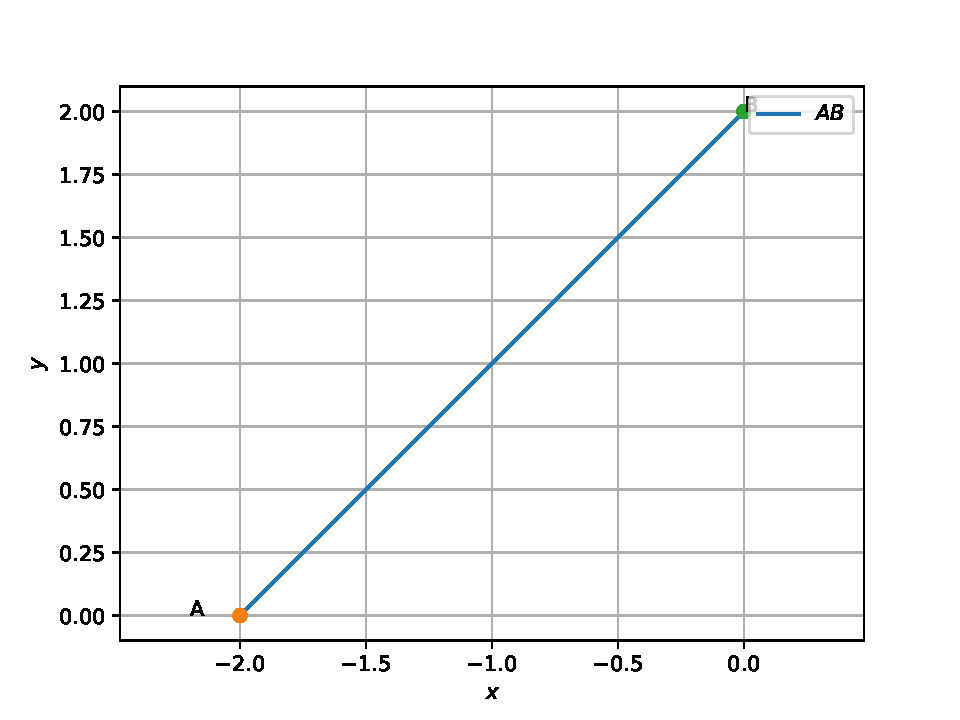
\includegraphics[width=\columnwidth]{./line/figs/line_zeros.eps}
\caption{}
\label{fig:line_zeros}
\end{figure}
%
\item Find a zero of the polynomial $p(x) = 2x + 1$.
\\
\solution $p\brak{-\frac{1}{2}} = 0$.
%
%
\item Find four different solutions of the equation 
\label{prob:line_icept}
%
\begin{align}
\label{eq:line_iceptx}
\myvec{1 & 2}\vec{x} &= 6
\end{align}
%
\solution Let 
%
\begin{align}
\vec{x} = \myvec{a\\0}
\end{align}
%
Substituting in \eqref{eq:line_iceptx}, 
%
\begin{align}
\myvec{1 & 2} \myvec{a\\0}&= 6
\\
\implies a &=6
\end{align}
%
Simiarly, substituting 
%
\begin{align}
\vec{x} &= \myvec{0\\b},
\end{align}
%
in \eqref{eq:line_iceptx}, 
%
%
\begin{align}
b =3
\end{align}
%
More solutions can be obtained in a similar fashion.
%
\item Draw the graph of 
%
\begin{align}
\myvec{1 & 1}\vec{x} &= 7
\end{align}
%
\solution The intercepts on the x and y-axis can be obtained from Problem \ref{prob:line_icept}
as
%
\begin{align}
\vec{A} = \myvec{7\\0}
\vec{B} = \myvec{0\\7}
\end{align}
%
The following python code can be used to draw the graph in Fig. \ref{fig:line_icept}.
%
\begin{lstlisting}
codes/line/line_icept.py
\end{lstlisting}
%
\begin{figure}[!ht]
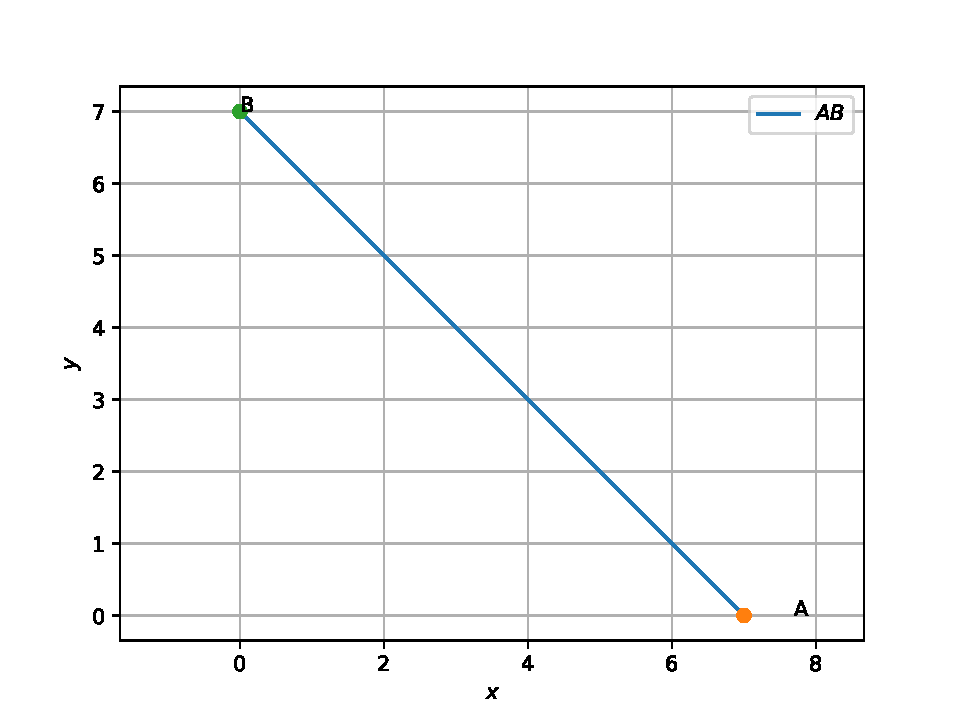
\includegraphics[width=\columnwidth]{./line/figs/line_icept.eps}
\caption{}
\label{fig:line_icept}
\end{figure}
%
%
\item Two rails are represented by the equations 
\label{prob:line_mat_eq}
\begin{align}
\label{eq:line_mat_eq}
\begin{split}
\myvec{1 & 2}\vec{x}  &= 4 \text{ and}
\\
\myvec{ 2 & 4}\vec{x} &=  12 . 
\end{split}
\end{align}
%
Will the rails cross each other?
%
\\
\solution The above equations can be expressed as the matrix equation
\begin{align}
\myvec{1 & 2\\2 & 4} \vec{x} = \myvec{4\\12}
\end{align}
%
The augmented matrix for the above equation is row reduced as follows
\begin{align}
\myvec{1 & 2 & 4\\2 & 4 & 12} 
\xleftrightarrow {R_2\leftarrow \frac{R_2}{2}}\myvec{1 & 2 & 4\\1 & 2 & 6} 
\\
%\myvec{1 & 2 & 4\\2 & 4 & 12} 
\xleftrightarrow {R_2\leftarrow R_2 - R_1}\myvec{1 & 2 & 4\\0 & 0 & 2} 
\label{eq:line_aug}
\end{align}
%
$\because$ row reduction of the $2\times 3$ matrix
%
\begin{align}
\myvec{1 & 2 & 4\\2 & 4 & 12} 
\end{align}
%
results in a matrix with 2 nonzero rows, its rank is 2.  Similarly, the rank of the matrix 
%
\begin{align}
\myvec{1 & 2\\2 & 4} 
\end{align}
is 1, from \ref{eq:line_aug}. 
%
\begin{align}
\because rank \myvec{1 & 2\\2 & 4} \ne rank\myvec{1 & 2 & 4\\2 & 4 & 12},  
\end{align}
%
\eqref{eq:line_mat_eq} has no solution.
%
The equivalent python code is
%
\begin{lstlisting}
codes/line/line_check_sol.py
\end{lstlisting}
%
which plots Fig. \ref{fig:line_check_sol}, which shows that the rails are parallel.
%
\begin{figure}[!ht]
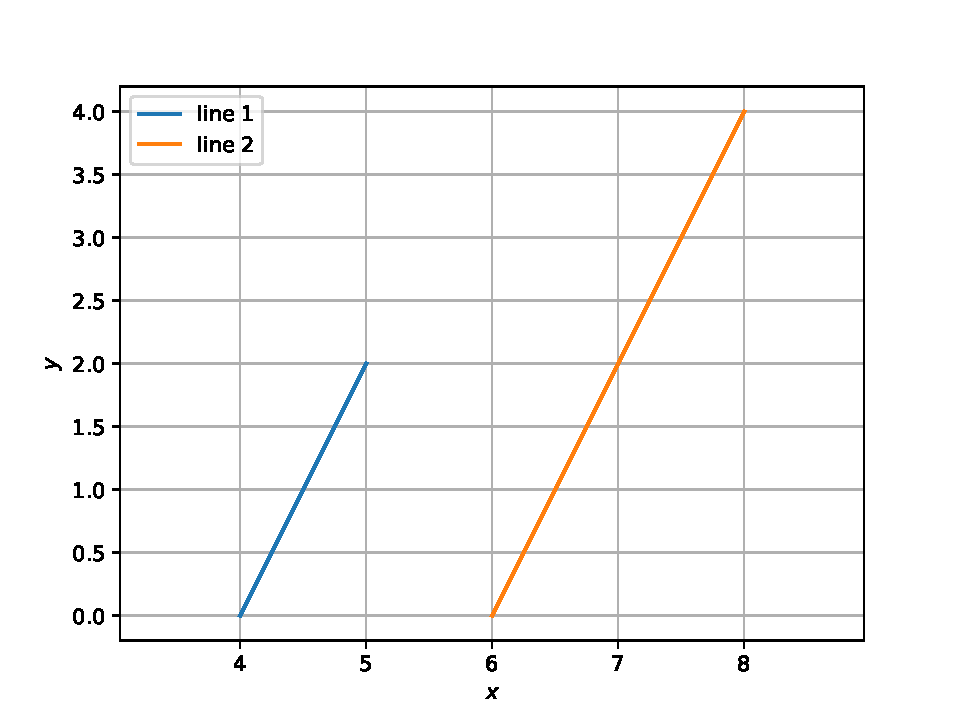
\includegraphics[width=\columnwidth]{./line/figs/line_check_sol.eps}
\caption{}
\label{fig:line_check_sol}
\end{figure}
%

\item Check whether the pair of equations 
\begin{align}
\label{eq:line_mat_eq_2}
\begin{split}
\myvec{1 & 3}\vec{x}  &= 6 \text{ and}
\\
\myvec{ 2 & -3}\vec{x} &= 12 
\end{split}
\end{align}
%
is consistent. 
\\
\solution The above equations can be expressed as the matrix equation
\begin{align}
\myvec{1 & 3\\2 & -3} \vec{x} = \myvec{6\\12}
\end{align}
%
The augmented matrix for the above equation is row reduced as follows
\begin{align}
\myvec{1 & 3 & 6\\2 & -3 & 12} 
\xleftrightarrow {R_2\leftarrow \frac{R_2-2R_1}{-9}}
%\myvec{1 & 3 & 6\\0 & -9 & 0} 
\\
\myvec{1 & 3 & 6\\0 & 1 & 0} 
\xleftrightarrow {R_1\leftarrow R_1 - 3R_2}\myvec{1 & 0 & 6\\0 & 1 & 0} 
\\
\implies \vec{x} = \myvec{6\\0}
\end{align}
%
which is the solution of \ref{eq:line_mat_eq}.
The python code in Problem \ref{prob:line_mat_eq}
%
%
can be used to plot Fig. \ref{fig:line_check_sol2}, which shows that the lines intersect.
%
\begin{figure}[!ht]
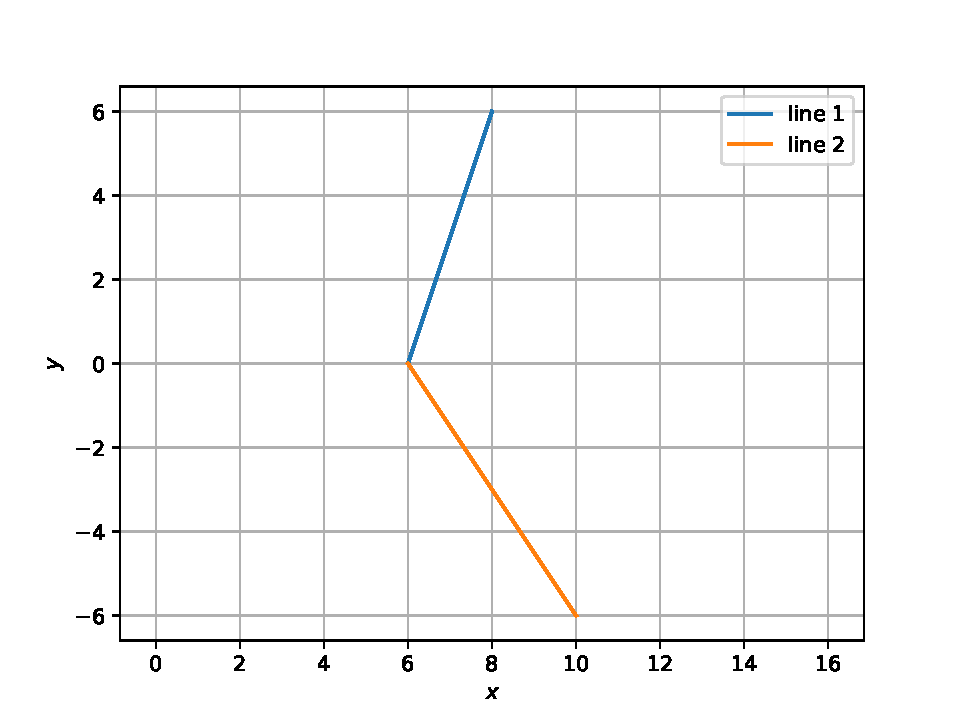
\includegraphics[width=\columnwidth]{./line/figs/line_check_sol2.eps}
\caption{}
\label{fig:line_check_sol2}
\end{figure}
%
%
\item Find whether the following pair of equations has no solution, unique solution or infinitely many solutions: 
%
\begin{align}
\label{eq:line_check_sol3}
\begin{split}
\myvec{5 & -8}\vec{x}  &= -1 \text{ and}
\\
\myvec{ 3 & -\frac{24}{5}}\vec{x} &= -\frac{3}{5}
\end{split}
\end{align}
%
\\
\solution The above equations can be expressed as the matrix equation
\begin{align}
\myvec{5 & -8\\3 & -\frac{24}{5}} \vec{x} = -\myvec{1\\ \frac{3}{5}}
\end{align}
%
The augmented matrix for the above equation is row reduced as follows
\begin{align}
\myvec{5 & -8 & -1 \\3 & -\frac{24}{5} & -\frac{3}{5}} 
\xleftrightarrow {R_2\leftarrow 5R_2}\myvec{5 & -8 & 1\\15 & -24 & -3} 
\\
%\myvec{5 & -8 & 1\\15 & -24 & -3} 
\xleftrightarrow {R_2\leftarrow R_2 - 3R_1}\myvec{5 & -8 & 1\\0 & 0 & 0} 
\end{align}
%
%
\begin{align}
\because rank \myvec{5 & -8\\3 & -\frac{24}{5}} &= rank \myvec{5 & -8 & 1 \\3 & -\frac{24}{5} & -\frac{3}{5}} 
\\
= 1 < dim \myvec{5 & -8\\3 & -\frac{24}{5}} =2,
\end{align}
%
\eqref{eq:line_check_sol3} has infinitely many solutions.
%
The python code in Problem \ref{prob:line_mat_eq}
%
%
can be used to plot Fig. \ref{fig:line_check_sol3}, which shows that the lines are the same.
%
\begin{figure}[!ht]
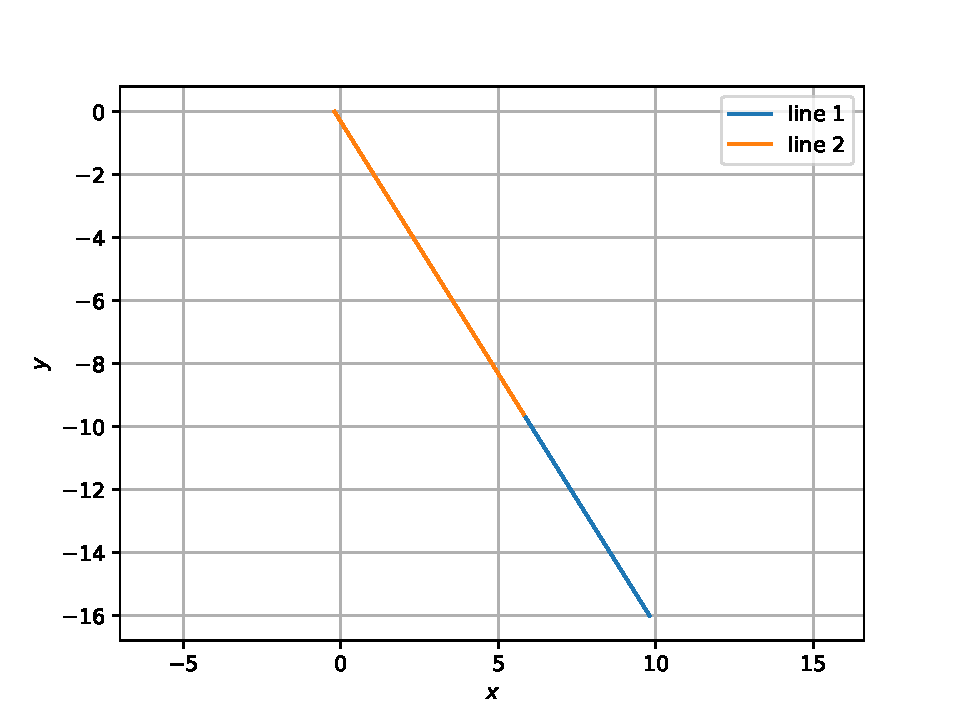
\includegraphics[width=\columnwidth]{./line/figs/line_check_sol3.eps}
\caption{}
\label{fig:line_check_sol3}
\end{figure}
%
%
\item Solve the following pair of equations
%
\begin{align}
\label{eq:line_check_sol_unique}
\myvec{7 & -15}\vec{x}  &= 2 
\\
\myvec{ 1 & 2}\vec{x} &= 3
\end{align}
%
\\
\solution The above equations can be expressed as the matrix equation
\begin{align}
\myvec{7 & -15\\1 & 2} \vec{x} = \myvec{2\\ 3}
\end{align}
%
The augmented matrix for the above equation is row reduced as follows
\begin{align}
\myvec{7 & -15 & 2\\1 & 2 & 3}
\xleftrightarrow {R_2\leftarrow 7R_2-R_1}\myvec{7 & -15 & 2\\0 & 29 & 19}
\\
\xleftrightarrow {R_1\leftarrow \frac{15R_2 29+ 29R_1}{29}}\myvec{7 & 0 & 2\\0 & 29 & 19} 
\\
\implies \vec{x} = \myvec{\frac{2}{7}\\\frac{19}{29}}
\end{align}
%
%

The python code in Problem \ref{prob:line_mat_eq}
%
%
can be used to plot Fig. \ref{fig:line_check_sol_unique}, which shows that the lines are the same.
%
\begin{figure}[!ht]
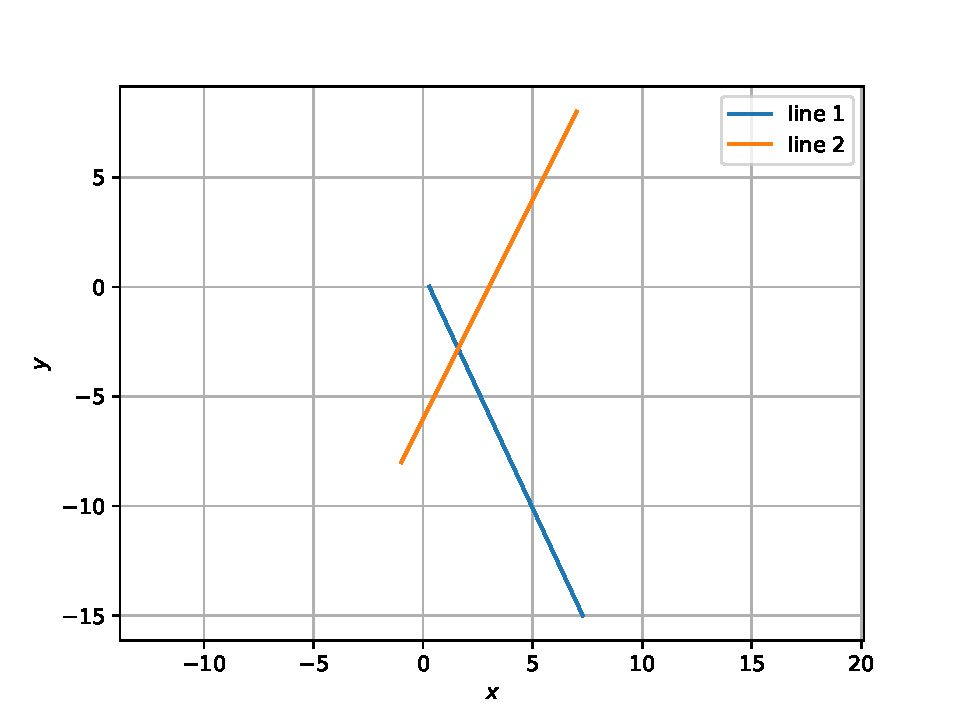
\includegraphics[width=\columnwidth]{./line/figs/line_check_unique.eps}
\caption{}
\label{fig:line_check_sol_unique}
\end{figure}
%
\item Find all possibe solutions of
\begin{align}
\label{eq:line_check_sol_nosol}
\begin{split}
\myvec{2 & 3 }\vec{x}&=8
\\
\myvec{4 & 6 }\vec{x}&=7
\end{split}
\end{align}
%
\\
\solution The above equations can be expressed as the matrix equation
\begin{align}
\myvec{2 & -3\\4 & 6} \vec{x} = \myvec{8\\ 7}
\end{align}
%
The augmented matrix for the above equation is row reduced as follows
\begin{align}
\myvec{2 & 3 & 8\\4 &  6 & 7} 
\xleftrightarrow {R_2\leftarrow R_2-2R_1}\myvec{2 & -3 & 8\\0 &  0 & -9} 
\\
\implies rank \myvec{2 & -3\\4 & 6} \ne \myvec{2 & 3 & 8\\4 &  6 & 7}. 
\end{align}
%
Hence, \eqref{eq:line_check_sol_nosol} has no solution.
The python code in Problem \ref{prob:line_mat_eq}
%
%
can be used to plot Fig. \ref{fig:line_check_nosol}, which shows that the lines are parallel.
%
\begin{figure}[!ht]
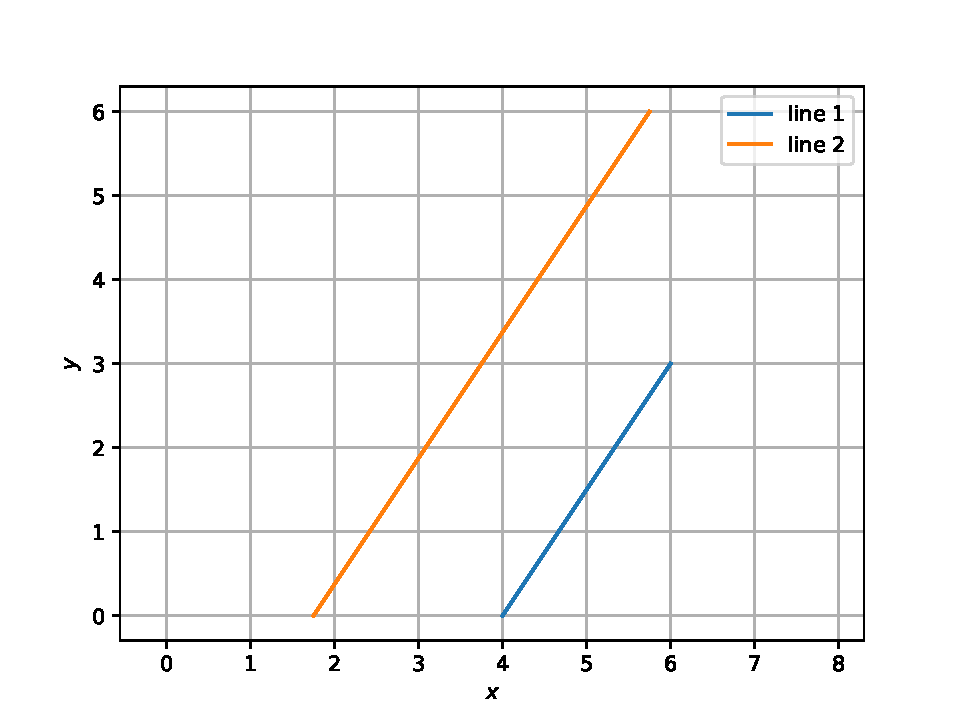
\includegraphics[width=\columnwidth]{./line/figs/line_check_nosol.eps}
\caption{}
\label{fig:line_check_nosol}
\end{figure}

\item For which values of p does the pair of equations given below has unique solution?
\begin{align}
\label{eq:line_det_unique}
\begin{split}
\myvec{4 & p }\vec{x}&=-8
\\
\myvec{2 & 2 }\vec{x}&=-2
\end{split}
\end{align}
%
\solution \eqref{eq:line_det_unique} has a unique solution 
\begin{align}
\iff \mydet{4 & p \\ 2 & 2} \ne 0
\\
\text{or, } p \ne 4
\end{align}
%
\item For what values of $k$ will the following pair of linear equations have infinitely many solutions?
%
\begin{align}
\label{eq:line_det_inf}
\begin{split}
\myvec{k & 3 }\vec{x}&=k-3
\\
\myvec{12 & k }\vec{x}&=k
\end{split}
\end{align}
%
\solution The first condition for \eqref{eq:line_det_inf} to have infinite solutions is 
%
\begin{align}
\label{eq:line_det_inf_cond}
\mydet{k & 3 \\12 & k  } &= 0
\\
\implies k^2 = 36, \text{or, } k = \pm 6
\end{align}
%
For $k = 6$, 
%
the augmented matrix for the above equation is row reduced as follows
\begin{align}
\myvec{6 & 3 & 3\\12 &  6 & 6} 
\xleftrightarrow {R_2\leftarrow R_2-2R_1}\myvec{6 & 3 & 3\\0 &  0 & 0} 
\end{align}
%
indicating that \eqref{eq:line_det_inf} has infinite number of solutions. For $k = -6$, the augmented matrix is 
\begin{align}
\myvec{6 & 3 & -9\\12 &  6 & -6} 
\xleftrightarrow {R_2\leftarrow R_2-2R_1}\myvec{6 & 3 & -9\\0 &  0 & 12} 
\end{align}
indicating that \eqref{eq:line_det_inf} has no solution
%
Thus, \eqref{eq:line_det_inf_cond} is a necessary condition but not sufficient.
%
%
%

\item Find the condition for $\vec{x} = \myvec{x_1\\x_2}$ to be equidistant from the points $\myvec{7\\1}, \myvec{3\\5}$.
\label{prob:line_perp_bisect}
%
\\
\solution From the given information,
%
\begin{align}
\norm{\vec{x}-\myvec{7\\1}}^2&=\norm{\vec{x}-\myvec{3\\5}}^2
\end{align}
\begin{multline}
\implies \norm{\vec{x}}^2 + \norm{\myvec{7\\1}}^2-2\myvec{7&1}\vec{x} 
\\= 
 \norm{\vec{x}}^2 + \norm{\myvec{3\\5}}^2-2\myvec{3&5}\vec{x} 
\end{multline}
%
which can be simplified to obtain
\begin{align}
\label{eq:line_p_bisect}
\myvec{1 & -1}\vec{x} = 2
\end{align}
%
which is the desired condition.  
The following code plots Fig. \ref{fig:line_perp_bisect}clearly showing that the above equation 
%\eqref{eq:line_p_bisect}
 is the perpendicular bisector of $AB$.

%
\begin{lstlisting}
codes/line/line_perp_bisect.py
\end{lstlisting}
%
\begin{figure}[!ht]
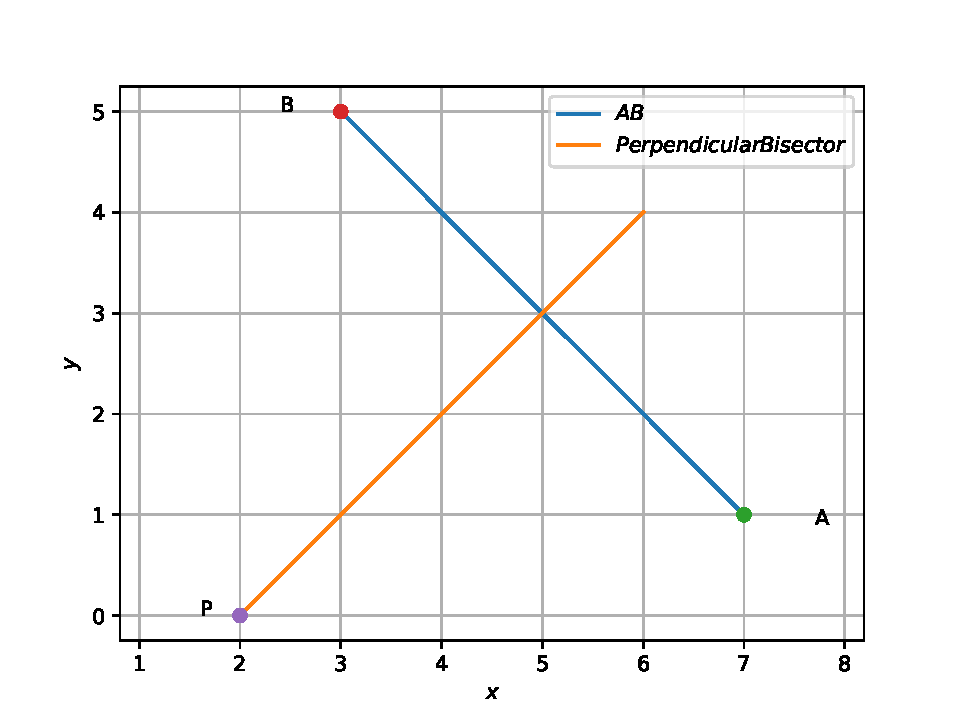
\includegraphics[width=\columnwidth]{./line/figs/line_perp_bisect.eps}
\caption{}
\label{fig:line_perp_bisect}
\end{figure}
%


\item Find the direction vectors and slopes of the lines passing through the points
%
\begin{enumerate}
\item \myvec{3\\-2} and \myvec{-1\\4}.
\item \myvec{3\\-2} and \myvec{7\\-2}.
\item \myvec{3\\-2} and \myvec{3\\4}.
\item Making an inclination of $60\degree$ with the positive direction of the x-axis.
\end{enumerate}
%
\solution
\begin{enumerate}
\item If the direction vector is 
\begin{align}
\myvec{1\\m}, 
\end{align}
%
the slope is $m$. Thus, the direction vector is
\begin{align}
\myvec{-1\\4} - \myvec{3\\-2} &= \myvec{-4\\6} = -\frac{1}{4} \myvec{-4\\6} 
\\
&=  \myvec{1\\-\frac{3}{2}} \implies m = -\frac{3}{2}
\end{align}
%
\item The direction vector is
\begin{align}
\myvec{7\\-2} - \myvec{3\\-2} &= \myvec{4\\0} 
\\
&=  \myvec{1\\0} \implies m = 0
\end{align}
%
\item The direction vector is
\begin{align}
\myvec{3\\4} - \myvec{3\\-2} &= \myvec{0\\6} 
\\
&=  \myvec{1\\ \infty} \implies m = \infty
\end{align}
%
\item The slope is $m = \tan 60 \degree = \sqrt{3}$ and the  direction vector is
\begin{align}
\myvec{1\\\sqrt{3}}
\end{align}
\end{enumerate}
\item If the angle between two lines is $\frac{\pi}{4}$ and the slope of one of the lines is $\frac{1}{4}$ find the slope of the other line.
\\
\solution The angle $\theta$ between two lines is given by 
%
\begin{align}
\tan \theta &= \frac{m_1-m_2}{1+m_1m_2}
\\
\implies 1 &= \frac{m_1-\frac{1}{4}}{1+\frac{m_1}{4}}
\\
\text{or } m_1 &= \frac{5}{3} 
\end{align}
%
%
%\\
%\solution 
%%Using \eqref{eq:tri_geo_ex_orth}
%\begin{align}
%\cbrak{\myvec{-2\\ 6}-\myvec{4\\8}}^T \cbrak{\myvec{8\\ 12}-\myvec{x\\24}}=  0 
%\end{align}
%%
%which can be used to obtain $x$.
\item Two positions of time and distance are recorded as, when $T = 0, D = 2$ and when $T = 3, D = 8$. Using the concept of slope, find law of motion, i.e., how distance depends upon time.
%
\\
\solution The equation of the line joining the points $\vec{A}=\myvec{0\\2}$ and $\vec{B}=\myvec{3\\8}$ is obtained as
%
\begin{align}
\label{eq:line_two_pt}
\vec{x} &= \vec{A}+\lambda\brak{\vec{B}-\vec{A}}
\\
\implies \myvec{T\\D} &= \myvec{0\\2}-\lambda\myvec{-3\\-6}
\end{align}
%
which can be expressed as
\begin{align}
\myvec{2 & -1}\myvec{T\\D} &= \myvec{2 & -1}\myvec{0\\2}\\
\implies \myvec{2 & -1}\myvec{T\\D} &= -2
\\
\implies D = 2+2T
\end{align}
%
\item Find the equations of the lines parallel to the axes and passing through $\vec{A}=\myvec{-2\\3}$.
%
\\
\solution The line parallel to the x-axis has direction vector $\vec{m}=\myvec{1\\0}$.  Hence,its equation is obtined as
\begin{align}
%
\label{eq:line_dir_vec}
\vec{x} = \myvec{-2\\3} + \lambda_1\myvec{1\\0}
\end{align}
%
Similarly, the equation of the line parallel to the y-axis can be obtained as
\begin{align}
\vec{x} = \myvec{-2\\3} + \lambda_1\myvec{0\\1}
\end{align}
%
The following code plots Fig. \ref{fig:line_parallel_axes}
%
\begin{lstlisting}
codes/line/line_parallel_axes.py
\end{lstlisting}
%
\begin{figure}[!ht]
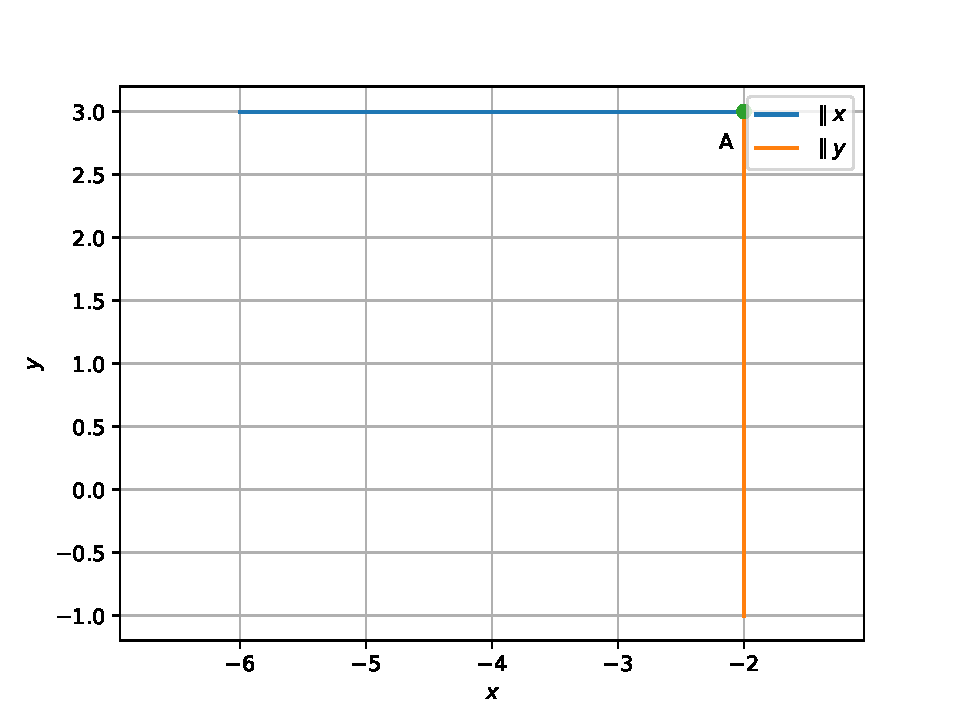
\includegraphics[width=\columnwidth]{./line/figs/line_parallel_axes.eps}
\caption{}
\label{fig:line_parallel_axes}
\end{figure}

\item Find the equation of the line through $\vec{A}=\myvec{– 2\\ 3}$ with slope –4.
\\
\solution The direction vector is $\vec{m} = \myvec{1\\-4}$.  Hence, the normal vector
\begin{align}
\label{eq:line_norm_dir}
\vec{n} &= \myvec{0&-1\\1&0}\vec{m} 
\\
&= \myvec{4\\1}
\end{align}
%
The equation of the line in terms of the normal vector is then obtained as
\begin{align}
\label{eq:line_norm_vec}
\vec{n}^T\brak{\vec{x}-\vec{A}} &= 0
\\
\implies \myvec{4 & 1} \vec{x} &= -5
\end{align}
%
\item Write the equation of the line through the points \myvec{1\\-1} and \myvec{3\\5}.
%
\\
\solution Use \eqref{eq:line_dir_vec}.
\item Write the equation of the lines for which $\tan \theta = \frac{1}{2}$, where $\theta$ is the inclination of the line and 
\label{prob:line_intercept}
\begin{enumerate}
\item y-intercept is $-\frac{3}{2}$
\item x-intercept is 4.
\end{enumerate}
%
\solution From the given information, $\tan \theta = \frac{1}{2}=m $.
\begin{enumerate}
\item y-intercept is $-\frac{3}{2} \implies $ the line cuts through the y-axis at $\myvec{0\\-\frac{3}{2}}$.
\item x-intercept is 4 $\implies$ the line cuts through the x-axis at $\myvec{4\\0}$.
\end{enumerate}
%
Use the above information get the equations for the lines.
%
\item Find the equation of a line through the point \myvec{5\\2\\-4} and parallel to the vector \myvec{3\\2\\-8}.
\\
\solution The equation of the line is 
\begin{align}
\vec{x} &= \myvec{5 & 2\\-4} + \lambda \myvec{3\\2\\-8}
\end{align}
%
\item Find the equation of a line passing through the points \myvec{-1\\0\\2} and \myvec{3\\4\\6}.
\\
\solution Using  \eqref{eq:line_two_pt}, the desired equation of the line is
\begin{align}
\vec{x} &= \myvec{-1 & 0\\2} + \lambda \myvec{4\\4\\4}
\\
&= \myvec{-1 & 0\\2} + \lambda \myvec{1\\1\\1}
\end{align}
%
\item If
\begin{align}
%
\label{eq:line_3d}
\frac{x+3}{2} = \frac{y-5}{4} = \frac{z+6}{2} = \lambda
\end{align}
%
find the equation of the line.
\label{prob:line_3d}
\\
\solution The line can be expressed from \eqref{eq:line_3d} as
%
\begin{align}
%\label{eq:line_3d}
\myvec{x\\y\\z} &= \myvec{-3+2\lambda\\5+4\lambda\\-6+2\lambda}
\\
\implies \vec{x} &= \myvec{-3\\5\\-6} + \lambda \myvec{2\\4\\2}
\\
\implies \vec{x} &= \myvec{-3\\5\\-6} + \lambda \myvec{1\\2\\1}
\end{align}
%
\item Find the equation of the line, which makes intercepts -3 and 2 on the x and y axes respectively.
\\
\solution See Problem \ref{prob:line_intercept}.  The line passes through the points \myvec{-3\\0} and \myvec{0\\2}.

\item Find the equation of the line whose perpendicular distance from the origin is 4 units and the angle which the normal makes with the positive direction of x-axis is $15\degree$.
%
\\
\solution  In Fig. \ref{fig:line_pt_dist}, the foot of the perpendicular $P$ is the intersection of the lines $L$ and $M$.  Thus, 
\begin{align}
\label{eq:line_pt_dist_foot}
\vec{n}^T\vec{P} &= c
\\
\label{eq:line_pt_dist_foot_normal}
\vec{P} = \vec{A} + \lambda\vec{n}
\\
\text{or, } \vec{n}^T\vec{P} = \vec{n}^T\vec{A} + \lambda\norm{\vec{n}}^2 = c
\\
\label{eq:line_pt_dist_lam}
\implies -\lambda = \frac{\vec{n}^T\vec{A}-c}{\norm{\vec{n}}^2}
\end{align}
%
Also, the distance between $\vec{A}$ and $L$ is obtained from 
%
\begin{align}
\vec{P} &= \vec{A} + \lambda\vec{n}
\\
\label{eq:line_pt_dist_lam_norm}
\implies \norm{\vec{P} - \vec{A}}  = \abs{\lambda}\norm{\vec{n}}
\end{align}
%
From \eqref{eq:line_pt_dist_lam}
and \eqref{eq:line_pt_dist_lam_norm}
%
\begin{align}
\label{eq:line_pt_dist}
\norm{\vec{P} - \vec{A}}  = \frac{\abs{\vec{n}^T\vec{A}-c}}{\norm{\vec{n}}}
\end{align}
%

\begin{figure}[!ht]
\includegraphics[width=\columnwidth]{./line/figs/line_pt_dist.eps}
\caption{}
\label{fig:line_pt_dist}
\end{figure}
%
\begin{align}
\vec{n} = \myvec{1\\\tan 15\degree}
\end{align}
%
$\because \vec{A} = \vec{0}$, 
\begin{align}
4 = \frac{\abs{ c}}{\norm{\vec{n}}} \implies c &= \pm 4\sqrt{1+\tan^2 15\degree} 
\\
&= \pm 4 \sec 15\degree
\end{align}
%
where 
%
\begin{align}
\sec \theta = \frac{1}{\cos \theta}
\end{align}
%
This follows from the fact that
%
\begin{align}
\cos^2 \theta + \sin^2 \theta &= 1
\\
\implies 1 + \frac{\sin^2 \theta}{\cos^2 \theta} &= \frac{1}{\cos^2 \theta}
\end{align}
%
It is easy to verify that 
%
\begin{align}
\frac{\sin \theta}{\cos \theta} &= \tan \theta
\\
\implies 1 + \tan^2 \theta &= \sec^2 \theta
\end{align}
%

Thus, the equation of the line is 
\begin{align}
\myvec{1 &\tan 15\degree} \vec{c} = \pm 4 \sec 15\degree
\end{align}
\item The Farenheit temperature $F$ and absolute temperature $K$ satisfy a linear equation.  Given $K=273$ when $F=32$ and that $K=373$  when $F=212$, express $K$ in terms of $F$ and find the value of $F$, when $K=0$.
%
\\
\solution Let 
\begin{align}
\vec{x}=\myvec{F & K} 
\end{align}
%
Since the relation between $F, K$ is linear, \myvec{273\\32}, \myvec{373\\21} are on a line.  The corresponding equation is obtained from \eqref{eq:line_norm_vec} and \eqref{eq:line_norm_dir} as 
%
\begin{align}
\myvec{11 & -100}\vec{x} &= \myvec{11 & -100}\myvec{273\\32} 
\\
\implies \myvec{11 & -100}\vec{x} &= -197
\end{align}
%
If \myvec{F\\0} is a point on the line, 
%
\begin{align}
\myvec{11 & -100}\myvec{F\\0} &= -197
\implies F = -\frac{197}{11}
\end{align}
%
\item Equation of a line is 
\begin{align}
\myvec{3 & – 4}\vec{x} + 10 = 0. 
\end{align}
Find its 
\begin{enumerate}
\item  slope, 
\item  x - and y-intercepts.
\end{enumerate}
%
\solution From the given information, 
%
\begin{align}
\vec{n} &= \myvec{3 \\ – 4}, 
\\
\vec{m} &= \myvec{4 \\ 3}, 
\end{align}
%
\begin{enumerate}
\item $m = \frac{3}{4}$
\item x-intercept is $-\frac{10}{3}$ and y-intercept is $\frac{10}{4} = \frac{5}{2}$.
\end{enumerate}
%
%
\item Find the angle between two vectors $\vec{a}$ and $\vec{b}$ where 
%
\begin{align}
\norm{\vec{a}} = 1,
\norm{\vec{b}} = 2,
\vec{a}^T\vec{b} = 1.
\end{align}
%
\solution In Fig. \ref{fig:line_scalar_prod}, from the cosine formula, 
%
\begin{align}
\cos \theta &= \frac{\norm{\vec{A}-\vec{B}}^2+\norm{\vec{B}-\vec{C}}^2-\norm{\vec{A}-\vec{C}}^2}{2\norm{\vec{A}-\vec{B}}\norm{\vec{B}-\vec{C}}}
\end{align}
Letting $\vec{a} = \vec{A}-\vec{B}, \vec{b} = \vec{B}-\vec{C}$, 
\begin{align}
\cos \theta &= \frac{\norm{\vec{a}}^2+\norm{\vec{b}}^2-\norm{\vec{a}+\vec{b}}^2}{2\norm{\vec{a}}\norm{\vec{b}}}
\\
&= \frac{\norm{\vec{a}}^2+\norm{\vec{b}}^2-\sbrak{\norm{\vec{a}}^2+\norm{\vec{b}}^2-2\vec{a}^T\vec{b}}}{2\norm{\vec{a}}\norm{\vec{b}}}
\\
\implies \cos \theta &=\frac{\vec{a}^T\vec{b}}{\norm{\vec{a}}\norm{\vec{b}}}
\end{align}
%
Thus, the angle $\theta$ between two vectors is given by 
%
\begin{align}
\label{eq:line_scalar_prod}
\cos \theta &= \frac{\vec{a}^T\vec{b}}{\norm{\vec{a}}\norm{\vec{b}}}
\\
&=\frac{1}{2}
\\
\implies \theta &= 60\degree
\end{align}
%
\begin{figure}[!ht]
\includegraphics[width=\columnwidth]{./line/figs/line_scalar_prod.eps}
\caption{}
\label{fig:line_scalar_prod}
\end{figure}
%


\item Find the angle between the lines 
%
\begin{align}
\myvec{1 & – \sqrt{3}}\vec{x}  = 5
\\
\myvec{\sqrt{3} & –1}\vec{x}  = -6
. 
\end{align}
%
\solution The angle between the lines can also be expressed in terms of the normal vectors as
%
\begin{align}
\cos \theta &= \frac{\vec{n}_1\vec{n}_2}{\norm{\vec{n}_1}\norm{\vec{n}_2}}
\\
&= \frac{\sqrt{3}}{2} \implies \theta = 30\degree
\end{align}
%
\item Find the equation of a line perpendicular to the line 
\begin{align}
\myvec{1 & – 2}\vec{x}  = 3
\end{align}
%
and passes through the point \myvec{1\\-2}.
%
\\
\solution The normal vector of the perpendicular line is 
%
\begin{align}
\myvec{2 \\ 1}
\end{align}
%
Thus, the desired equation of the line is 
%
\begin{align}
\myvec{2 & 1}\brak{\vec{x} - \myvec{1\\-2}} &=0
\\
\implies \myvec{2 & 1}\vec{x} =0
\end{align}
%

\item Find the distance of the point \myvec{3\\-5} from the line 
\begin{align}
\myvec{3 & – 4}\vec{x}  = 26
\end{align}
%
\solution Use \eqref{eq:line_pt_dist}.

\item If the lines 
\begin{align}
\myvec{2 & 1}\vec{x}  = 3
\\
\myvec{5 & k}\vec{x}  = 3
\\
\myvec{3 & -1}\vec{x}  = 2
\end{align}
%
are concurrent, find the value of $k$.
%
\\
\solution If the lines are concurrent, the {\em augmented}  matrix should have a 0 row upon row reduction.  Hence, 
%
\begin{align}
\myvec{
2 & 1 & 3
\\
5 & k & 3
\\
3 & -1 & 2
}
\xleftrightarrow{R_2\leftrightarrow R_3}
\myvec{
2 & 1 & 3
\\
3 & -1 & 2
\\
5 & k & 3
}
\\
\xleftrightarrow [R_3\leftarrow 2R_3-5R_1]{R_2\leftrightarrow 2R_2-3R_1}
\myvec{
2 & 1 & 3
\\
0 & -5 & -5
\\
0 & 2k-5 & -9
}
\\
\xleftrightarrow []{R_2\leftarrow -\frac{R_2}{5}}
\myvec{
2 & 1 & 3
\\
0 & 1 & 1
\\
0 & 2k-5 & -9
}
\\
\xleftrightarrow []{R_3\leftarrow R_3-\brak{2k-5}R_2}
\myvec{
2 & 1 & 3
\\
0 & 1 & 1
\\
0 & 0 & -2k-4
}
\\
\implies k = -2
\end{align}
%
\item Find the distance of the line
\begin{align}
\label{eq:line_L_1}
L_1: \quad \myvec{4 & 1}\vec{x}  = 0
\end{align}
%
from the point \myvec{4\\1} measured along the line $L_2$ making an angle of $135\degree$ with the positive x-axis.
%
\\
\solution  Let $P$ be the point of intersection of $L_1$ and $L_2$.  The direction vector of $L_2$ is 
\begin{align}
\vec{m} = \myvec{1 \\ \tan 135\degree}
\end{align}
%
Since \myvec{4\\1} lies on $L_2$, the equation of $L_2$ is 
\begin{align}
\label{eq:line_L_2}
\vec{x} &= \myvec{4\\1} + \lambda \vec{m} 
\\
\label{eq:line_L_2_P}
\implies \vec{P} &= \myvec{4\\1} + \lambda \vec{m} 
\\
\label{eq:line_L_2_P_dist}
\text{or, } \norm{\vec{P} - \myvec{4\\1}} &= d = \abs{\lambda}\norm{\vec{m} }
%
\end{align}
%
Since $\vec{P}$ lies on $L_1$, from \eqref{eq:line_L_1},
%
\begin{align}
\myvec{4 & 1}\vec{P}  = 0
\end{align}
%
Substituting from the above in \eqref{eq:line_L_2},
%
\begin{align}
\myvec{4 & 1}\myvec{4\\1} + \lambda \myvec{4 & 1}\vec{m}  &= 0
\\
\implies \lambda &= \frac{\myvec{4 & 1}\vec{m}}{17}
\end{align}
%
substituting $\abs{\lambda}$ in \eqref{eq:line_L_2_P_dist} gives the desired answer.

\item Assuming that straight lines work as a plane mirror for a point, find the image of the point \myvec{1\\2} in the line 
%
\begin{align}
\myvec{1 & -3}\vec{x}  = -4.
\end{align}
%
%\item Find $\vec{R}$, the {\em reflection}  of $\vec{P}$ about the line
%\begin{align}
%L: \quad \vec{n}^T\vec{x} = c
%\end{align}
%
\begin{figure}
\centering
\includegraphics[width=\columnwidth]{./line/figs/reflection.eps}
\caption{}
\label{fig:line_reflection}
\end{figure}
\solution Since $\vec{R}$ is the reflection of $\vec{P}$ and $\vec{Q}$ lies on $L$, $\vec{Q}$ bisects $PR$.  
This leads to the following equations
\begin{align}
\label{eq:reflect_bisect}
2\vec{Q} &= \vec{P}+\vec{R}
\\
\label{eq:reflect_Q}
\vec{n}^{T}\vec{Q} &= c
\\
\label{eq:reflect_R}
\vec{m}^{T}\vec{R} &= \vec{m}^{T}\vec{P}
\end{align}
%
where $\vec{m}$ is the direction vector of $L$.  From \eqref{eq:reflect_bisect} and \eqref{eq:reflect_Q},
\begin{align}
\label{eq:reflect_bisectQ}
\vec{n}^{T}\vec{R}  &= 2c - \vec{n}^{T}\vec{P}
\end{align}
%
From \eqref{eq:reflect_bisectQ} and \eqref{eq:reflect_R},
\begin{align}
\label{eq:reflect_bisectQR}
\myvec{\vec{m} & \vec{n}}^T\vec{R} &= \myvec{\vec{m} & -\vec{n}}^T\vec{P}+ \myvec{0 \\ 2c}
\end{align}
%
Letting 
\begin{align}
\label{eq:reflect_mat}
\vec{V}=  \myvec{\vec{m} & \vec{n}}
\end{align}
with the condition that $\vec{m},\vec{n}$ are orthonormal, i.e.
\begin{align}
\label{eq:reflect_ortho}
\vec{V}^T\vec{V}=  \vec{I}
\end{align}
%
Noting that 
\begin{align}
\label{eq:reflect_trans}
\myvec{\vec{m} & -\vec{n}} &= \myvec{\vec{m} & \vec{n}} \myvec{1 & 0 \\ 0 & -1},
\end{align}
\eqref{eq:reflect_bisectQR} can be expressed as
%
\begin{align}
\label{eq:reflect_}
\vec{V}^T\vec{R} &=  \sbrak{\vec{V}\myvec{1 & 0 \\ 0 & -1}}^T\vec{P}+\myvec{0 \\ 2c}
\\
\implies \vec{R} &= \sbrak{\vec{V}\myvec{1 & 0 \\ 0 & -1}\vec{V}^{-1}}^T\vec{P}+ \vec{V}\myvec{0 \\ 2c}
\\
 &=\vec{V}\myvec{1 & 0 \\ 0 & -1}\vec{V}^T \vec{P}+2c \vec{n}
\end{align}
It can be verified that 
%\item Show that, for any $\vec{m},\vec{n}$, 
the reflection is also given by
\begin{align}
%\label{eq:reflect_bisect}
\frac{\vec{R}}{2} = \frac{\vec{m}\vec{m}^T-\vec{n}\vec{n}^T}{\vec{m}^T\vec{m}+\vec{n}^T\vec{n}}\vec{P} + c 
\frac{\vec{n}}{\norm{\vec{n}}^2}
\end{align}
%\solution The reflection of a point $\vec{P}$ about a line 
%%
%\begin{align}
%\vec{n}^T\vec{x}  = c
%\end{align}
%%
%is given by $\vec{R}$, where
%\begin{align}
%\label{eq:line_reflect}
%\frac{\vec{R}}{2} = \frac{\vec{m}\vec{m}^T-\vec{n}\vec{n}^T}{\vec{m}^T\vec{m}+\vec{n}^T\vec{n}}\vec{P} + c \frac{\vec{n}}{\norm{\vec{n}}^2}
%\end{align}
%
The following code plots Fig. \ref{fig:line_reflect} while computing the reflection
%
\begin{lstlisting}
codes/line/line_reflect.py
\end{lstlisting}
%
\begin{figure}[!ht]
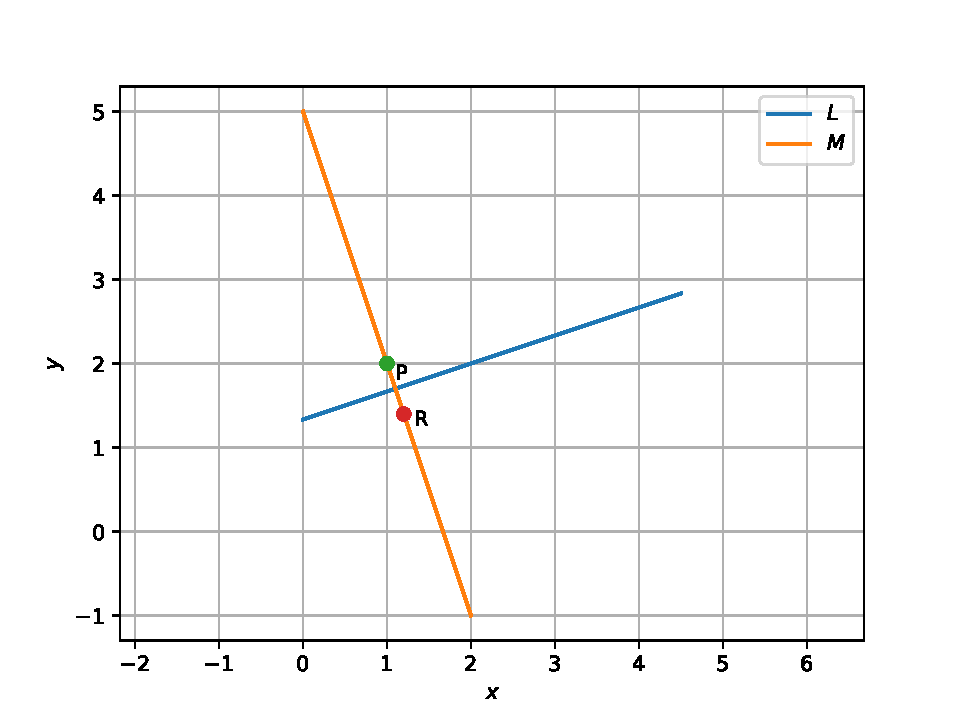
\includegraphics[width=\columnwidth]{./line/figs/line_reflect.eps}
\caption{}
\label{fig:line_reflect}
\end{figure}
%

\item A line $L$ is such that its segment between the lines %
is bisected at the point $\vec{P} = \myvec{1\\5}$.  Obtain its equation.
\begin{align}
\label{eq:line_seg}
L_1: \quad \myvec{5 & -1}\vec{x}  &= -4
\\
L_2: \quad \myvec{3 & 4}\vec{x}  &= 4
\end{align}
%
\\
\solution Let 
%
\begin{align}
L: \quad \vec{x}  &= \vec{P} + \lambda \vec{m}
\end{align}
%
If $L$ intersects $L_1$ and $L_2$ at $\vec{A}$ and $\vec{B}$ respectively, 
%
\begin{align}
\label{eq:line_segA}
 \vec{A}  &= \vec{P} + \lambda \vec{m}
\\
 \vec{B}  &= \vec{P} - \lambda \vec{m}
\label{eq:line_segB}
\end{align}
%
since $\vec{P}$ bisects $AB$. Note that $\lambda$ is a measure of the distance from $P$  along the line $L$.
%
From \eqref{eq:line_seg}, \eqref{eq:line_segA} and \eqref{eq:line_segB},
%
\begin{align}
\myvec{5 & -1} \vec{A}  &= \myvec{5 & -1}\myvec{1\\5} + \lambda \myvec{5 & -1}\vec{m}=-4
\\
\myvec{3 & 4} \vec{B}  &= \myvec{3 & 4}\myvec{1\\5} - \lambda \myvec{3 & 4}\vec{m}=4
\end{align}
%
yielding
%
\begin{align}
19\myvec{5 & -1}\vec{m}&=-4 \myvec{3 & 4}\vec{m}
\\
\implies \myvec{107 & -3}\vec{m} &= 0
\\
\text{or, } \vec{n} = \myvec{107\\-3}
\end{align}
%
after simplification.
Thus, the equation of the line is 
\begin{align}
\vec{n}^T\brak{\vec{x}-\vec{P}} =0
\end{align}
\item Show that the path of a moving point such that its distances from two lines
%
\begin{align}
\myvec{3 & -2}\vec{x}  &= 5
\\
\myvec{3 & 2}\vec{x}  &= 5
\end{align}
%
are  equal is a straight line.
%
\\
\solution Using \eqref{eq:line_pt_dist} the point $\vec{x}$ satisfies
%
\begin{align}
\frac{\abs{\myvec{3 & -2}\vec{x}  - 5}}{\norm{\myvec{3 \\ -2}}}
&=\
\frac{\abs{\myvec{3 & 2}\vec{x}  - 5}}{\norm{\myvec{3 \\ 2}}}
\\
\implies \abs{\myvec{3 & -2}\vec{x}  - 5}&=\abs{\myvec{3 & 2}\vec{x}  - 5}
\end{align}
%
resulting in 
%
\begin{align}
\myvec{3 & -2}\vec{x}  - 5=\pm\brak{\myvec{3 & 2}\vec{x}  - 5}
\end{align}
%
leading to the possible lines
%
\begin{align}
L_1: \quad \myvec{0 & 1}\vec{x}  &=0
\\
L_2: \quad \myvec{1 & 0}\vec{x}  &=  \frac{5}{3}
\end{align}
%
\item Find the angle between the vectors 
$\vec{a}=\myvec{1\\1\\-1}$
  and 
$\vec{b}=\myvec{1\\-1\\1}$.
%
\\
\solution 
From theory, we understand that using dot product we can find the angle between the lines 
\begin{enumerate}
	\item 
	\begin{align}\label{eq:solutions/line_plane/74/codes:5}
		\frac{x-2}{2} = \frac{y-1}{5} &= \frac{z+3}{-3}, 
	\end{align}
	\begin{align}\label{eq:solutions/line_plane/74/codes:6}
		\frac{x+2}{-1} = \frac{y-4}{8} &= \frac{z-5}{4} 
	\end{align}


The above symmetric equations \ref{eq:solutions/line_plane/74/codes:5}, \ref{eq:solutions/line_plane/74/codes:6} can be represented in the vector form as 
\begin{align}\label{eq:solutions/line_plane/74/codes7}
	\quad \vec{r_1} &= \myvec{2\\1\\-3} + \lambda_1\myvec{2\\5\\-3}
	\\
	\quad \vec{r_2} &= \myvec{-2\\4\\5} + \lambda_2\myvec{-1\\8\\4}
\end{align}

As we have to find the angle between the vectors, we will only be taking the direction vectors into consideration. The direction vectors are $\vec{u}$ = $\myvec{2\\5\\-3}$ and $\vec{v}$ = $\myvec{-1\\8\\4}$. We can find the corresponding magnitude values

\begin{align}\label{eq:solutions/line_plane/74/codes9}
	\norm{\vec{u}} =\sqrt{2^{2}+5^{2}+(-3)^{2}} =\sqrt{38}
\end{align}
\begin{align}\label{eq:solutions/line_plane/74/codes10}
	\norm{\vec{v}} =\sqrt{(-1)^{2}+8^{2}+4^{2}} =\sqrt{81}
\end{align}

Using \ref{eq:solutions/line_plane/74/codes4}, \ref{eq:solutions/line_plane/74/codes9}, \ref{eq:solutions/line_plane/74/codes10} we get
\begin{align}
	\theta = \cos ^{-1}\frac{\myvec{2\\5\\-3}^{T}\myvec{-1\\8\\4}}{(\sqrt{38})(\sqrt{81})} 
	\\
	\theta = \cos ^{-1}\frac{26}{55.4797}
	\\
	\theta = \cos ^{-1} (0.4686)
	\\
	\theta = 62.053\degree
\end{align}

Therefore, the angle between the two lines is $62.053\degree$.See Fig. \ref{fig:solutions/line_plane/74/codesline_equation_1}

\begin{figure}
	\centering
	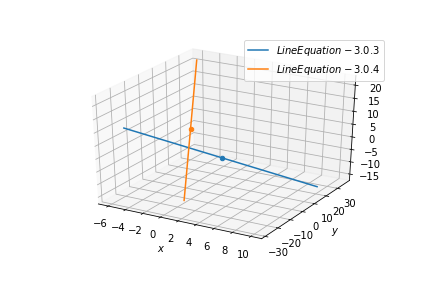
\includegraphics[width=\columnwidth]{./solutions/line_plane/74/codes/figs/Line_interest_1.png}
	\caption{Graph for equations \ref{eq:solutions/line_plane/74/codes7}}
	\label{fig:solutions/line_plane/74/codesline_equation_1}
\end{figure}


	\item 
	\begin{align}\label{eq:solutions/line_plane/74/codes12}
		\frac{x}{2} = \frac{y}{2} &= \frac{z}{1}, 
	\end{align}
	\begin{align}\label{eq:solutions/line_plane/74/codes13}
		\frac{x-5}{4} = \frac{y-2}{1} &= \frac{z-3}{8} 
	\end{align}



The above symmetric equations \ref{eq:solutions/line_plane/74/codes12}, \ref{eq:solutions/line_plane/74/codes13} can be represented in the vector form as 
\begin{align}\label{eq:solutions/line_plane/74/codes14}
	\quad \vec{r_1} &= \myvec{0\\0\\0} + \lambda_1\myvec{2\\2\\1}
	\\
	\quad \vec{r_2} &= \myvec{5\\2\\3} + \lambda_2\myvec{4\\1\\8}
\end{align}

As we have to find the angle between the vectors, we will only be taking the direction vectors into consideration. The direction vectors are $\vec{u}$ = $\myvec{2\\2\\1}$ and $\vec{v}$ = $\myvec{4\\1\\8}$. We can find the corresponding magnitude values

\begin{align}\label{eq:solutions/line_plane/74/codes16}
	\norm{\vec{u}} =\sqrt{2^{2}+2^{2}+1^{2}} =\sqrt{9}
\end{align}
\begin{align}\label{eq:solutions/line_plane/74/codes17}
	\norm{\vec{v}} =\sqrt{4^{2}+1^{2}+8^{2}} =\sqrt{81}
\end{align}

Using \ref{eq:solutions/line_plane/74/codes4}, \ref{eq:solutions/line_plane/74/codes16}, \ref{eq:solutions/line_plane/74/codes17} we get
\begin{align}
	\theta = \cos ^{-1}\frac{\myvec{2\\2\\1}^{T}\myvec{4\\1\\8}}{(\sqrt{9})(\sqrt{81})} 
	\\
	\theta = \cos ^{-1}\frac{18}{27.00}
	\\
	\theta = \cos ^{-1} (0.667)
	\\
	\theta = 48.189\degree
\end{align}

Therefore, the angle between the two lines is $48.189\degree$. See Fig. \ref{fig:solutions/line_plane/74/codesline_equation_2}


\begin{figure}
	\centering
	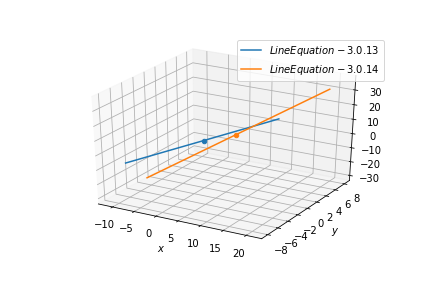
\includegraphics[width=\columnwidth]{./solutions/line_plane/74/codes/figs/Line_interest_2.png}
	\caption{Graph for equations \ref{eq:solutions/line_plane/74/codes14}}
	\label{fig:solutions/line_plane/74/codesline_equation_2}
\end{figure}
\end{enumerate}

    

%
\item Find the angle between the pair of lines given by 
\begin{align}
\vec{x} &= \myvec{3\\2\\-4} + \lambda_1\myvec{1 \\ 2 \\2}
\\
\vec{x} &= \myvec{5\\-2\\0} + \lambda_2\myvec{3 \\ 2 \\6}
\end{align}
%
\\
\solution 
From theory, we understand that using dot product we can find the angle between the lines 
\begin{enumerate}
	\item 
	\begin{align}\label{eq:solutions/line_plane/74/codes:5}
		\frac{x-2}{2} = \frac{y-1}{5} &= \frac{z+3}{-3}, 
	\end{align}
	\begin{align}\label{eq:solutions/line_plane/74/codes:6}
		\frac{x+2}{-1} = \frac{y-4}{8} &= \frac{z-5}{4} 
	\end{align}


The above symmetric equations \ref{eq:solutions/line_plane/74/codes:5}, \ref{eq:solutions/line_plane/74/codes:6} can be represented in the vector form as 
\begin{align}\label{eq:solutions/line_plane/74/codes7}
	\quad \vec{r_1} &= \myvec{2\\1\\-3} + \lambda_1\myvec{2\\5\\-3}
	\\
	\quad \vec{r_2} &= \myvec{-2\\4\\5} + \lambda_2\myvec{-1\\8\\4}
\end{align}

As we have to find the angle between the vectors, we will only be taking the direction vectors into consideration. The direction vectors are $\vec{u}$ = $\myvec{2\\5\\-3}$ and $\vec{v}$ = $\myvec{-1\\8\\4}$. We can find the corresponding magnitude values

\begin{align}\label{eq:solutions/line_plane/74/codes9}
	\norm{\vec{u}} =\sqrt{2^{2}+5^{2}+(-3)^{2}} =\sqrt{38}
\end{align}
\begin{align}\label{eq:solutions/line_plane/74/codes10}
	\norm{\vec{v}} =\sqrt{(-1)^{2}+8^{2}+4^{2}} =\sqrt{81}
\end{align}

Using \ref{eq:solutions/line_plane/74/codes4}, \ref{eq:solutions/line_plane/74/codes9}, \ref{eq:solutions/line_plane/74/codes10} we get
\begin{align}
	\theta = \cos ^{-1}\frac{\myvec{2\\5\\-3}^{T}\myvec{-1\\8\\4}}{(\sqrt{38})(\sqrt{81})} 
	\\
	\theta = \cos ^{-1}\frac{26}{55.4797}
	\\
	\theta = \cos ^{-1} (0.4686)
	\\
	\theta = 62.053\degree
\end{align}

Therefore, the angle between the two lines is $62.053\degree$.See Fig. \ref{fig:solutions/line_plane/74/codesline_equation_1}

\begin{figure}
	\centering
	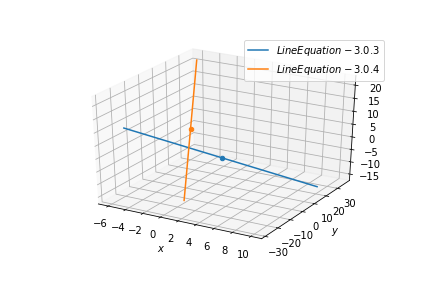
\includegraphics[width=\columnwidth]{./solutions/line_plane/74/codes/figs/Line_interest_1.png}
	\caption{Graph for equations \ref{eq:solutions/line_plane/74/codes7}}
	\label{fig:solutions/line_plane/74/codesline_equation_1}
\end{figure}


	\item 
	\begin{align}\label{eq:solutions/line_plane/74/codes12}
		\frac{x}{2} = \frac{y}{2} &= \frac{z}{1}, 
	\end{align}
	\begin{align}\label{eq:solutions/line_plane/74/codes13}
		\frac{x-5}{4} = \frac{y-2}{1} &= \frac{z-3}{8} 
	\end{align}



The above symmetric equations \ref{eq:solutions/line_plane/74/codes12}, \ref{eq:solutions/line_plane/74/codes13} can be represented in the vector form as 
\begin{align}\label{eq:solutions/line_plane/74/codes14}
	\quad \vec{r_1} &= \myvec{0\\0\\0} + \lambda_1\myvec{2\\2\\1}
	\\
	\quad \vec{r_2} &= \myvec{5\\2\\3} + \lambda_2\myvec{4\\1\\8}
\end{align}

As we have to find the angle between the vectors, we will only be taking the direction vectors into consideration. The direction vectors are $\vec{u}$ = $\myvec{2\\2\\1}$ and $\vec{v}$ = $\myvec{4\\1\\8}$. We can find the corresponding magnitude values

\begin{align}\label{eq:solutions/line_plane/74/codes16}
	\norm{\vec{u}} =\sqrt{2^{2}+2^{2}+1^{2}} =\sqrt{9}
\end{align}
\begin{align}\label{eq:solutions/line_plane/74/codes17}
	\norm{\vec{v}} =\sqrt{4^{2}+1^{2}+8^{2}} =\sqrt{81}
\end{align}

Using \ref{eq:solutions/line_plane/74/codes4}, \ref{eq:solutions/line_plane/74/codes16}, \ref{eq:solutions/line_plane/74/codes17} we get
\begin{align}
	\theta = \cos ^{-1}\frac{\myvec{2\\2\\1}^{T}\myvec{4\\1\\8}}{(\sqrt{9})(\sqrt{81})} 
	\\
	\theta = \cos ^{-1}\frac{18}{27.00}
	\\
	\theta = \cos ^{-1} (0.667)
	\\
	\theta = 48.189\degree
\end{align}

Therefore, the angle between the two lines is $48.189\degree$. See Fig. \ref{fig:solutions/line_plane/74/codesline_equation_2}


\begin{figure}
	\centering
	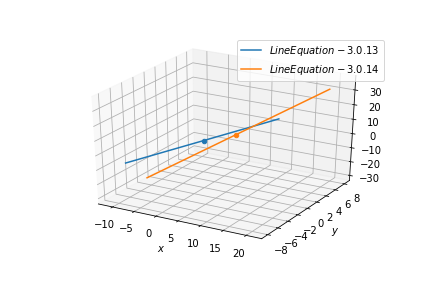
\includegraphics[width=\columnwidth]{./solutions/line_plane/74/codes/figs/Line_interest_2.png}
	\caption{Graph for equations \ref{eq:solutions/line_plane/74/codes14}}
	\label{fig:solutions/line_plane/74/codesline_equation_2}
\end{figure}
\end{enumerate}

    

\item Find the angle between the pair of lines
\begin{align}
\frac{x+3}{3} = \frac{y-1}{5} &= \frac{z+3}{4}, 
\\
\frac{x+1}{1} = \frac{y-4}{1} &= \frac{z-5}{2} 
\end{align}
%
\\
\solution 
From theory, we understand that using dot product we can find the angle between the lines 
\begin{enumerate}
	\item 
	\begin{align}\label{eq:solutions/line_plane/74/codes:5}
		\frac{x-2}{2} = \frac{y-1}{5} &= \frac{z+3}{-3}, 
	\end{align}
	\begin{align}\label{eq:solutions/line_plane/74/codes:6}
		\frac{x+2}{-1} = \frac{y-4}{8} &= \frac{z-5}{4} 
	\end{align}


The above symmetric equations \ref{eq:solutions/line_plane/74/codes:5}, \ref{eq:solutions/line_plane/74/codes:6} can be represented in the vector form as 
\begin{align}\label{eq:solutions/line_plane/74/codes7}
	\quad \vec{r_1} &= \myvec{2\\1\\-3} + \lambda_1\myvec{2\\5\\-3}
	\\
	\quad \vec{r_2} &= \myvec{-2\\4\\5} + \lambda_2\myvec{-1\\8\\4}
\end{align}

As we have to find the angle between the vectors, we will only be taking the direction vectors into consideration. The direction vectors are $\vec{u}$ = $\myvec{2\\5\\-3}$ and $\vec{v}$ = $\myvec{-1\\8\\4}$. We can find the corresponding magnitude values

\begin{align}\label{eq:solutions/line_plane/74/codes9}
	\norm{\vec{u}} =\sqrt{2^{2}+5^{2}+(-3)^{2}} =\sqrt{38}
\end{align}
\begin{align}\label{eq:solutions/line_plane/74/codes10}
	\norm{\vec{v}} =\sqrt{(-1)^{2}+8^{2}+4^{2}} =\sqrt{81}
\end{align}

Using \ref{eq:solutions/line_plane/74/codes4}, \ref{eq:solutions/line_plane/74/codes9}, \ref{eq:solutions/line_plane/74/codes10} we get
\begin{align}
	\theta = \cos ^{-1}\frac{\myvec{2\\5\\-3}^{T}\myvec{-1\\8\\4}}{(\sqrt{38})(\sqrt{81})} 
	\\
	\theta = \cos ^{-1}\frac{26}{55.4797}
	\\
	\theta = \cos ^{-1} (0.4686)
	\\
	\theta = 62.053\degree
\end{align}

Therefore, the angle between the two lines is $62.053\degree$.See Fig. \ref{fig:solutions/line_plane/74/codesline_equation_1}

\begin{figure}
	\centering
	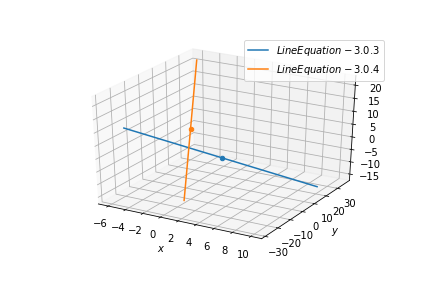
\includegraphics[width=\columnwidth]{./solutions/line_plane/74/codes/figs/Line_interest_1.png}
	\caption{Graph for equations \ref{eq:solutions/line_plane/74/codes7}}
	\label{fig:solutions/line_plane/74/codesline_equation_1}
\end{figure}


	\item 
	\begin{align}\label{eq:solutions/line_plane/74/codes12}
		\frac{x}{2} = \frac{y}{2} &= \frac{z}{1}, 
	\end{align}
	\begin{align}\label{eq:solutions/line_plane/74/codes13}
		\frac{x-5}{4} = \frac{y-2}{1} &= \frac{z-3}{8} 
	\end{align}



The above symmetric equations \ref{eq:solutions/line_plane/74/codes12}, \ref{eq:solutions/line_plane/74/codes13} can be represented in the vector form as 
\begin{align}\label{eq:solutions/line_plane/74/codes14}
	\quad \vec{r_1} &= \myvec{0\\0\\0} + \lambda_1\myvec{2\\2\\1}
	\\
	\quad \vec{r_2} &= \myvec{5\\2\\3} + \lambda_2\myvec{4\\1\\8}
\end{align}

As we have to find the angle between the vectors, we will only be taking the direction vectors into consideration. The direction vectors are $\vec{u}$ = $\myvec{2\\2\\1}$ and $\vec{v}$ = $\myvec{4\\1\\8}$. We can find the corresponding magnitude values

\begin{align}\label{eq:solutions/line_plane/74/codes16}
	\norm{\vec{u}} =\sqrt{2^{2}+2^{2}+1^{2}} =\sqrt{9}
\end{align}
\begin{align}\label{eq:solutions/line_plane/74/codes17}
	\norm{\vec{v}} =\sqrt{4^{2}+1^{2}+8^{2}} =\sqrt{81}
\end{align}

Using \ref{eq:solutions/line_plane/74/codes4}, \ref{eq:solutions/line_plane/74/codes16}, \ref{eq:solutions/line_plane/74/codes17} we get
\begin{align}
	\theta = \cos ^{-1}\frac{\myvec{2\\2\\1}^{T}\myvec{4\\1\\8}}{(\sqrt{9})(\sqrt{81})} 
	\\
	\theta = \cos ^{-1}\frac{18}{27.00}
	\\
	\theta = \cos ^{-1} (0.667)
	\\
	\theta = 48.189\degree
\end{align}

Therefore, the angle between the two lines is $48.189\degree$. See Fig. \ref{fig:solutions/line_plane/74/codesline_equation_2}


\begin{figure}
	\centering
	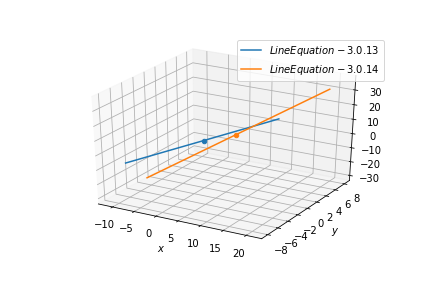
\includegraphics[width=\columnwidth]{./solutions/line_plane/74/codes/figs/Line_interest_2.png}
	\caption{Graph for equations \ref{eq:solutions/line_plane/74/codes14}}
	\label{fig:solutions/line_plane/74/codesline_equation_2}
\end{figure}
\end{enumerate}

    

%
\item Find a unit vector that makes an angle of $90\degree, 60\degree$ and $30\degree$ with the positive x, y and z axis respectively.
%
\\
\solution
The direction vector is
%
\begin{align}
\label{eq:line_dir_cos}
\vec{x} &= \myvec{\cos 90\degree\\\cos 60\degree \\ \cos 30\degree} = \myvec{0 \\ \frac{1}{2}\\\frac{\sqrt{3}}{2}}
\end{align}
%
$\because \norm{\vec{x}}=1$, it is the desired unit vector.
%
\item Find the 
distance between the lines 
\begin{align}
L_1: \quad \vec{x} &= \myvec{1\\2\\-4} + \lambda_1\myvec{2 \\ 3 \\6}
\\
L_2: \quad \vec{x} &= \myvec{3\\3\\-5} + \lambda_2\myvec{2 \\ 3 \\6}
\end{align}
\label{prob:line_dist_parallel}
%
\solution Both the lines have the same direction vector, so the lines are parallel. 
The following code plots 
%
\begin{lstlisting}
codes/line/line_dist_parallel.py
\end{lstlisting}
Fig. \ref{fig:line_dist_parallel_py} 
%
\begin{figure}[!ht]
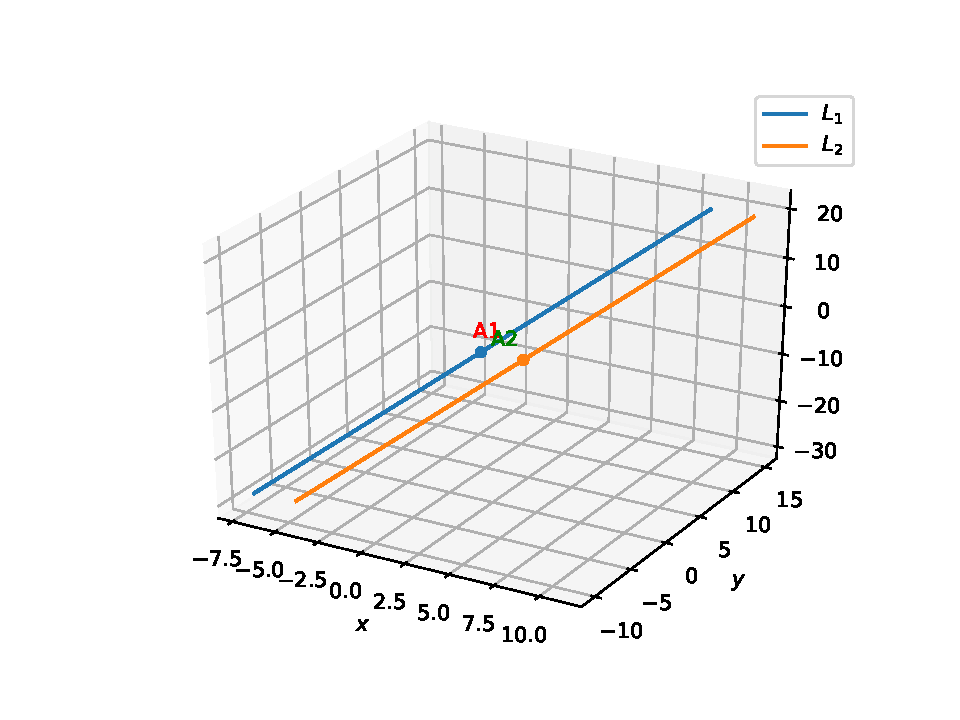
\includegraphics[width=\columnwidth]{./line/figs/line_dist_parallel_py.eps}
\caption{}
\label{fig:line_dist_parallel_py}
\end{figure}
%
%
From Fig. \ref{fig:line_dist_parallel}, the distance is
%
\begin{figure}
\centering
\includegraphics[width=\columnwidth]{./line/figs/line_dist_parallel.eps}
\caption{}
\label{fig:line_dist_parallel}
\end{figure}
%
\begin{align}
\label{eq:line_dist_parallel}
\vec{\norm{\vec{A}_2-
\vec{A}_1}}\sin\theta =\frac{\norm{\vec{m}\times \brak{\vec{A}_2-
\vec{A}_1}}}{\norm{\vec{m}}}
\end{align}
%
where 
%
\begin{align}
\vec{A}_1 = \myvec{1\\2\\-4},
\vec{A}_2 = \myvec{3\\3\\-5},
\vec{m}=\myvec{2 \\ 3 \\6}
\end{align}
%

\item Find the shortest distance between the lines 
\begin{align}
L_1: \quad \vec{x} &= \myvec{1\\1\\0} + \lambda_1\myvec{2 \\ -1 \\1}
\\
L_2: \quad \vec{x} &= \myvec{2\\1\\-1} + \lambda_2\myvec{3 \\ -5 \\2}
\end{align}
\label{prob:line_dist_skew}
%
\solution  In the given  problem
\begin{align}
\vec{A}_1= \myvec{1\\1\\0}, \vec{m}_1=\myvec{2 \\ -1 \\1},
\vec{A}_2= \myvec{2\\1\\-1}, \vec{m}_2 =\myvec{3 \\ -5 \\2}.
\end{align}
%
The lines will intersect if
%
\begin{align}
\myvec{1\\1\\0} + \lambda_1\myvec{2 \\ -1 \\1}
= \myvec{2\\1\\-1} + \lambda_2\myvec{3 \\ -5 \\2}
\\
\implies \lambda_1\myvec{2 \\ -1 \\1} - \lambda_2\myvec{3 \\ -5 \\2} &= \myvec{2\\1\\-1}-\myvec{1\\1\\0}  
\\
\implies \myvec{2 & 3 \\ -1 & -5 \\ 1 & 2}\myvec{\lambda_1\\ \lambda_2} = \myvec{1\\0\\-1}
\end{align}
%
Row reducing the augmented matrix,
%
\begin{align}
\myvec{
2 & 3 & 1 
\\
-1 & -5 & 0
\\
1 & 2 & -1
}
\xleftrightarrow[]{R_3\leftrightarrow R_1}
\myvec{
1 & 2 & -1
\\
-1 & -5 & 0
\\
2 & 3 & 1 
}
\\
\xleftrightarrow[]{\substack{R_2= R_1+R_2\\R_3 = 2R_1-R_3}}
\myvec{
1 & 2 & -1
\\
0 & -3 & -1
\\
0 & 1 & -3 
}
\xleftrightarrow[]{R_2\leftrightarrow R_3}
\myvec{
1 & 2 & -1
\\
0 & 1 & -3 
\\
0 & -3 & -1
}
\\
\xleftrightarrow[]{R_3=3R_2+R_3}
\myvec{
1 & 2 & -1
\\
0 & 1 & -3 
\\
0 & 0 & -10
}
\end{align}
%
The above matrix has $rank = 3$.  Hence, the lines do not intersect.  Note that the lines are not parallel but they  lie on parallel planes.  Such lines are known as {\em skew} lines.  
The following code plots 
Fig. \ref{fig:line_dist_skew} 
%
\begin{lstlisting}
codes/line/line_dist_skew.py
\end{lstlisting}
%
\begin{figure}[!ht]
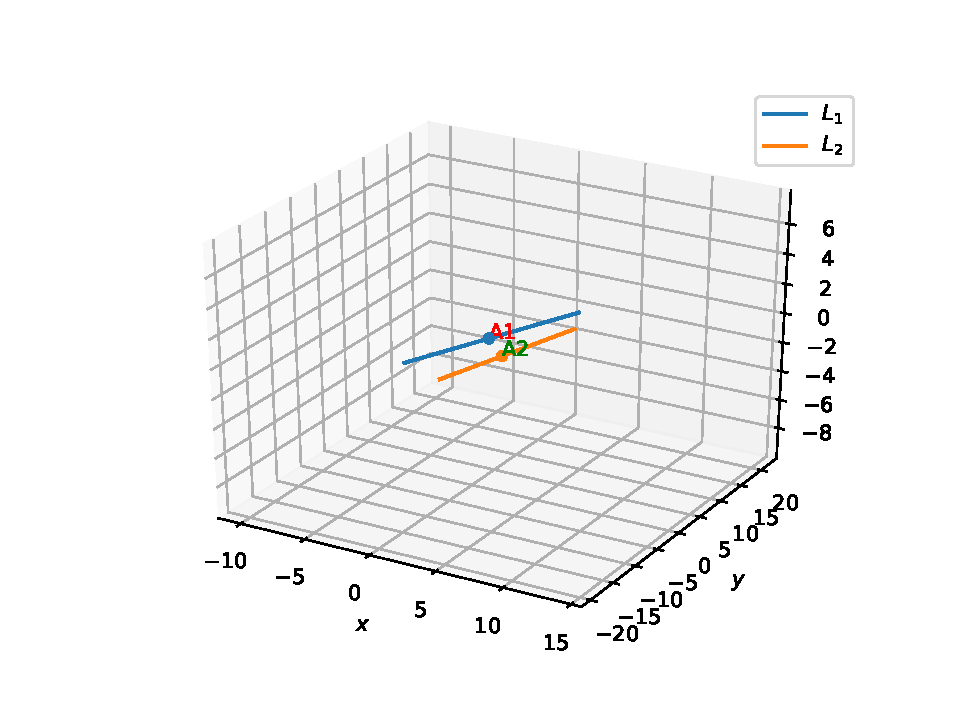
\includegraphics[width=\columnwidth]{./line/figs/line_dist_skew.eps}
\caption{}
\label{fig:line_dist_skew}
\end{figure}
%

The normal to both the lines (and corresponding planes) is 
%
\begin{align}
\label{eq:line_dist_skew_normal}
\vec{n} = \vec{m}_1\times\vec{m}_2
\end{align}
%
The equation of the second plane is then obtained as
%
\begin{align}
\label{eq:line_dist_skew_plane2}
\vec{n}^T \vec{x} = \vec{n}^T \vec{A}_2 
\end{align}
%
The distance from $\vec{A}_1$ to the above line is then obtained using 
\eqref{eq:line_pt_dist} as
%
\begin{align}
\label{eq:line_dist_skew}
\frac{\abs{\vec{n}^T\brak{\vec{A}_2-\vec{A}_1}}}{\norm{\vec{n}}}
=
\frac{\abs{\brak{\vec{A}_2-\vec{A}_1}^T\brak{\vec{m}_1\times\vec{m}_2}}}{\norm{\vec{m}_1\times\vec{m}_2}}
\end{align}
%

\item Find the distance of the plane 
\begin{align}
\myvec{2 & -3 & 4}\vec{x}-6  = 0
\end{align}
%
from the origin.
\\
\solution From \eqref{eq:line_pt_dist}, the distance is obtained as
%
\begin{align}
\frac{\abs{c}}{\norm{\vec{n}}} &= \frac{6}{\sqrt{2^2+3^2+4^2}}
\\
&= \frac{6}{\sqrt{29}}
\end{align}
%

\item Find the equation of a plane which is at a distance of $\frac{6}{\sqrt{29}}$ from the origin and has  normal vector $\vec{n}=\myvec{2\\-3\\4}$.
%
\\
\solution From the previous problem, the desired equation is
%
\begin{align}
\myvec{2 & -3 & 4}\vec{x}-6  = 0
\end{align}
%

\item Find the unit normal vector of the plane 
\begin{align}
\myvec{6 & -3 & -2}\vec{x}  = 1.
\end{align}
%
\solution The normal vector is 
%
\begin{align}
\vec{n} = \myvec{6 & -3 & -2}
\\
\because \norm{\vec{n}} = 7,
\end{align}
%
the unit normal vector is 
%
\begin{align}
\frac{\vec{n}}{\norm{\vec{n}}} = \frac{1}{7}\myvec{6 & -3 & -2}
\end{align}
%
\item Find the coordinates of the foot of the perpendicular drawn from the origin to the plane 
\begin{align}
\label{eq:line_foot_perp}
\myvec{2 & -3 & 4}\vec{x}-6  = 0
\end{align}
%
\solution The normal vector is 
%
\begin{align}
\vec{n}=\myvec{2 \\ -3 \\ 4}
\end{align}
%
Hence, the foot of the perpendicular from the origin is $\lambda \vec{n}$.  Substituting in \eqref{eq:line_foot_perp},
\begin{align}
\lambda \norm{\vec{n}}^2 = 6  \implies \lambda = \frac{6}{\norm{\vec{n}}^2} = \frac{6}{29}
\end{align}
%
Thus, the foot of the perpendicular is
%
\begin{align}
\frac{6}{29}\myvec{2 \\ -3 \\ 4}
\end{align}
%
\item Find the equation of the plane which passes through the point $\vec{A}=\myvec{5\\2\\-4}$ and perpendicular to the line with direction vector $\vec{n}=\myvec{2\\3\\-1}$.
%
\\
\solution  The normal vector to the plane is $\vec{n}$. Hence from \eqref{eq:line_norm_vec}, the equation of the plane is 
%
\begin{align}
\vec{n}^T\brak{\vec{x}-\vec{A}} &= 0
\\
\implies \myvec{2\\3\\-1}\vec{x} &=\myvec{2&3&-1}\myvec{5\\2\\-4}
\\
&=20
\end{align}
%
%The following 
%%
%\begin{lstlisting}
%codes/line/plane_3d.py
%\end{lstlisting}
%%
%\begin{figure}[!ht]
%\includegraphics[width=\columnwidth]{./line/figs/plane_3d.eps}
%\caption{}
%\label{fig:plane_3d}
%\end{figure}
%

\item Find the equation of the plane passing through 
$
\bm{R} = \myvec{2\\5\\-3},
\bm{S}= \myvec{-2\\-3\\5}
$ 
and 
$
\bm{T}= \myvec{5\\3\\-3}.
$
\label{prob:plane_3pts}
\\
\solution  If the equation of the plane be 
\begin{align}
\vec{n}^T\vec{x} &= c,
\\
\vec{n}^T\vec{R}=\vec{n}^T\vec{S}=\vec{n}^T\vec{T}&= c,
\\
\implies \myvec{\vec{R}-\vec{S} & \vec{S}-\vec{T}}^T\vec{n} &= 0
\end{align}
%
after some algebra.
Using row reduction on the above matrix, 
\begin{align}
\myvec{4 & 8 &-8 \\ -7  & -6 & 8} \xleftrightarrow[]{R_1\leftarrow \frac{R_1}{4}}\myvec{1 & 2 &-2 \\ -7  & -6 & 8}
\\
\xleftrightarrow[]{R_2\leftarrow R_2 + 7R_1}
\myvec{
1 & 2 &-2 
\\ 
0  & 8 & -6
}
\xleftrightarrow[]{R_2\leftarrow \frac{R_2}{2}}
\myvec{
1 & 2 &-2 
\\ 
0  & 4 & -3
}
\\
\xleftrightarrow[]{R_1\leftarrow 2R_1-R_2}
\myvec{
2 & 0 &-1 
\\ 
0  & 4 & -3
}
\end{align}
%
Thus, 
\begin{align}
\vec{n} &= \myvec{\frac{1}{2}\\\frac{3}{4}\\1} = \myvec{2\\3\\4} \text{ and}
\\
c = \vec{n}^{T}\vec{T} = 7
\end{align}
%
Thus, the equation of the plane is 
%
\begin{align}
\myvec{2 & 3 & 4}\vec{n} = 7
\end{align}
%
Alternatively, the normal vector to the plane can be obtained as
%
\begin{align}
\vec{n} = \brak{\vec{R}-\vec{S}} \times \brak{\vec{S}-\vec{T}}
\end{align}
%
The equation of the plane is then obtained from \eqref{eq:line_norm_vec} as 
%
\begin{align}
\label{eq:plane_3pts_cross}
\vec{n}^T\brak{\vec{x}-\vec{T}} = \sbrak{\brak{\vec{R}-\vec{S}} \times \brak{\vec{S}-\vec{T}}}^T\brak{\vec{x}-\vec{T}} = 0
\end{align}
%

\item Find the equation of the plane with intercepts 2, 3 and 4 on the x, y and z axis respectively.
\\
\solution From the given information, the plane passes through the points \myvec{2\\0\\0}, \myvec{0\\3\\0} and \myvec{0\\0\\4} respectively. The equation can be obtained using Problem \ref{prob:plane_3pts}.

\item Find the equation of the plane passing through the intersection of the planes 
%
\begin{align}
\label{eq:plane_2p_1pt_1}
\myvec{1 & 1 & 1}\vec{x}&=6  
\\
\myvec{2 & 3 & 4}\vec{x}&=-5
\label{eq:plane_2p_1pt_2}
\end{align}
%
and the point \myvec{1\\1\\1}.
\\
\solution The intersection of the planes is obtained by row reducing the augmented matrix as
%
\begin{align}
\myvec{
1 & 1 & 1 & 6
\\
2 & 3 & 4 & -5
}
\xleftrightarrow[]{R_2 = R_2 -2R_1}
\myvec{
1 & 1 & 1 & 6
\\
0 & 1 & 2 & -17
}
\\
\xleftrightarrow[]{R_1 = R_1 -R_2}
\myvec{
1 & 0 & -1 & 23
\\
0 & 1 & 2 & -17
}
\\
\implies 
\vec{x} = \myvec{23\\-17\\0}+\lambda\myvec{1\\-2\\1}
\end{align}
%
Thus, \myvec{23\\-17\\0} is another point on the plane.  The normal vector to the plane is then obtained as
The normal vector to the plane is then obtained as
%
\begin{align}
\brak{ \myvec{1\\1\\1}-\myvec{23\\-17\\0}}\times \myvec{1\\-2\\1} 
\end{align}
%
which can be obtained by row reducing the matrix
\begin{align}
\myvec{
1 & -2 & 1
\\
-22 & 18 & 1
}
\xleftrightarrow[]{R_2 = R_2+22R_1}
\myvec{
1 & -2 & 1
\\
0  & -26 & 23
}
\\
\xleftrightarrow[]{R_1 = 13R_1-R_2}
\myvec{
13 & 0 & -10
\\
0  & -26 & 23
}
\\
\implies \vec{n} = \myvec{\frac{10}{13}\\\frac{23}{26}\\1} = \myvec{20\\23\\26}
\end{align}
%
Since the plane passes through \myvec{1\\1\\1}, using 
 \eqref{eq:line_norm_vec},
%
\begin{align}
\myvec{20 & 23 & 26}\brak{\vec{x}- \myvec{1\\1\\1}} &= 0
\\
\implies 
\myvec{20 & 23 & 26}\vec{x} &= 69
\end{align}
%
Alternatively, the plane passing through the intersection of \eqref{eq:plane_2p_1pt_1} and 
\eqref{eq:plane_2p_1pt_2} has the form 
%
\begin{align}
\label{eq:plane_2p_1pt_lam}
\myvec{1 & 1 & 1}\vec{x} + \lambda \myvec{2 & 3 & 4}\vec{x} &=6 -5\lambda  
\end{align}
%
Substituting \myvec{1\\1\\1} in the above, 
%
\begin{align}
\myvec{1 & 1 & 1}\myvec{1\\1\\1} + \lambda \myvec{2 & 3 & 4}\myvec{1\\1\\1} &=6 -5\lambda  
\\
\implies 3 + 9\lambda &= 6-5\lambda
\\
\implies &\lambda = \frac{3}{14}
\end{align}
%
Substituting this value of $\lambda $ in \eqref{eq:plane_2p_1pt_lam} yields the equation of the plane.

\item Show that the lines 
\label{prob:line_coplanar}
%
\begin{align}
\frac{x+3}{-3} = \frac{y-1}{1} &= \frac{z-5}{5}, 
\\
\frac{x+1}{-1} = \frac{y-2}{2} &= \frac{z-5}{5} 
\end{align}
%
are coplanar.
\\
\solution Since the given lines have different direction vectors, they are not parallel.  From Problem \eqref{prob:line_dist_skew}, the lines are coplanar if the distance between them is 0, i.e. they intersect.  This is possible if 
%
\begin{align}
\label{eq:line_coplanar}
\brak{\vec{A}_2-\vec{A}_1}^T\brak{\vec{m}_1\times\vec{m}_2} = 0
\end{align}
%
From the given information, 
%
\begin{align}
\vec{A}_2-\vec{A}_1 = \myvec{-3\\1\\5}-\myvec{-1\\2\\5} = \myvec{-2\\-1\\0}
\end{align}
%
$\vec{m}_1\times \vec{m}_2$ is obtained by row reducing the matrix
%
\begin{align}
\myvec{
-1 & 2 & 5
\\
-3 & 1 & 5
}
\xleftrightarrow[]{R_2=\frac{R_2-3R_1}{5}}
\myvec{
-1 & 2 & 5
\\
0 & 1 & 2
}
\\
\xleftrightarrow[]{R_1=-R_1+2R_2}
\myvec{
1 & 0 & -1
\\
0 & 1 & 2
}
\implies \myvec{-1 \\ 2 \\ 5}
\times \myvec{-3 \\ 1 \\ 5}
=\myvec{1\\-2\\1}
\end{align}
%
The LHS of \eqref{eq:line_coplanar} is 
\begin{align}
\myvec{-2 & -1 & 0}
\myvec{1\\-2\\1} = 0
\end{align}
%
which completes the proof.  Alternatively, the lines are coplanar if
%
\begin{align}
\mydet{\vec{A}_1-\vec{A}_2 & \vec{m}_1 & \vec{m}_2} = 0
\end{align}
%

\item Find the angle between the two planes
\label{prob:planes_angle}
\begin{align}
\myvec{2 & 1 & -2}\vec{x}&=5
\\
\myvec{3 &-6 & -2}\vec{x}&=7.
\end{align}
%
\solution The angle between two planes is the same as the angle between their normal vectors.  This can be obtained from \eqref{eq:line_scalar_prod}.

\item Find the angle between the two planes
\begin{align}
\myvec{2 & 2 & -2}\vec{x}&=5
\\
\myvec{3 &-6 & 2}\vec{x}&=7.
\end{align}
%
\solution See Problem \eqref{prob:planes_angle}.
%
\item Find the distance of a point \myvec{2\\5\\-3} from the plane
\begin{align}
\myvec{6 & -3 & 2}\vec{x}=4
\end{align}
%
\\
\solution Use \eqref{eq:line_pt_dist}.
\item Find the angle between the line 
%
\begin{align}
L: \quad \frac{x+1}{2} = \frac{y}{3} = \frac{z-3}{6} 
\end{align}
%
and
%
the plane 
\begin{align}
P: \quad \myvec{10 & 2 & -11}\vec{x}=3
\end{align}
%
\label{prob:plane_angle_line}
%
\solution The angle between the direction vector of $L$ and normal vector of $P$ is 
%
\begin{align}
\cos \theta &= \frac{\abs{\myvec{10 & 2 & -11}\myvec{2\\3\\6}}}{\sqrt{225}\times \sqrt{49}} = \frac{8}{21}
\end{align}
%
Thus, the desired angle is $90\degree -\theta$.
\item Find the equation of the plane that contains the point $\myvec{1\\-1\\2}$ and is perpedicular to each of the planes
\begin{align}
\myvec{2 & 3 & -2}\vec{x}&=5
\\
\myvec{1 & 2 & -3}\vec{x}&=8
\end{align}
%
\solution The normal vector to the desired plane is $\perp$ the normal vectors of both the given planes.  Thus,
%
\begin{align}
\vec{n} = \myvec{2 \\ 3 \\ -2} \times \myvec{1 \\ 2 \\ -3}
\end{align}
%
The equation of the plane is then obtained as
%
\begin{align}
\vec{n}^T\brak{\vec{x}-\vec{A}} = 0
\end{align}
%
\item Find the distance between the point $\vec{P}=\myvec{6\\5\\9}$ and the plane determined by the points $\bm{A}=\myvec{3\\-1\\2}, \bm{B}=\myvec{5\\2\\4}$ and $\bm{C}=\myvec{-1\\-1\\6}$.
%
\\
\solution Find the equation of the plane using Problem \ref{prob:plane_3pts}.  Find the distance using \eqref{eq:line_pt_dist}.
%
\item Find the coordinates of the point where the line through the points
$
\vec{A}=\myvec{3\\4\\1}, 
\vec{B}=\myvec{5\\1\\6}
$
crosses the XY plane.
%
\\
\solution The equation of the line is 
%
\begin{align}
\vec{x} &= \vec{A}+\lambda\brak{\vec{B}-\vec{A}}
\\
&= \myvec{3\\4\\1} + \lambda \myvec{2\\-3\\5}
\end{align}
%
The line  crosses the XY plane for $x_3 = 0 \implies \lambda = -\frac{1}{5}$. Thus, the desired point is
%
\begin{align}
 \myvec{3\\4\\1} -\frac{1}{5}\myvec{2\\-3\\5} = \frac{1}{5}\myvec{13\\23\\0}
\end{align}
%
\item Show that the function given by $f(x) = 7x – 3$ is increasing on $\vec{R}$.
\\
\solution A function is said to be increasing if
\begin{align}
x_2> x_1 &\implies f(x_2)> f(x_1)
\\
\implies \frac{f(x_2)-f(x_1)}{x_2 - x_1}  &> 0
\label{eq:line_inc_12}
\end{align}
%
Letting $x_1 = x, x_2 = x+h$ in \eqref{eq:line_inc_12}, this results in 
\begin{align}
\frac{f(x+h)-f(x)}{h} > 0
\label{eq:line_slope}
\end{align}
In the given problem, 
\begin{align}
\frac{f(x+h)-f(x)}{h} = 7 > 0
\end{align}
%
Hence, the given function is increasing.
%
%
\item A funcion $f(x)$ is increasing if 
\label{them:inc_der_def}
\begin{align}
f^{\prime}(x)=\lim_{h\to 0} \frac{f(x+h)-f(x)}{h} & > 0
\end{align}
%
$f^{\prime}(x)$ is defined as the {\em derivative} of $f(x)$.
The function is decreasing if $f^{\prime}(x) < 0$.  
%
\item The funcion $f(x) = ax+b, a \ne 0$ is increasing if $f^{\prime}(x) = a > 0$.  Else, it is decreasing.
\label{them:line_inc}
%

\item Find the maximum and minimum values, if any, of the function given by 
%
\begin{align}
\label{eq:line_der_def_prob}
f(x) = x, x \in \brak{0,1}.
\end{align}
%
\solution It is easy to verify that $f^{\prime}(x) = 1 > 0$ in the given interval.    Hence, the function is increasing.   The maximum value in the given interval is 1 and the minimum value is 0.
%
\item Find all points of local maxima and local minima of the function $f$ given by 
%
\begin{align}
\label{eq:line_abs}
f(x)  = 3 +\abs{x}, \quad x \in \vec{R}
\end{align}
%
\solution \eqref{eq:line_abs} can be expressed as 
%
\begin{align}
\label{eq:line_abs_cases}
f(x)  = 
\begin{cases}
3 +x & x > 0
\\
0 & x = 0
\\
3- x & < 0
\end{cases}
\end{align}
%
From Theorem \ref{them:line_inc}, 
%
\begin{align}
%\label{eq:line_abs_cases}
f^{\prime}(x)  = 
\begin{cases}
1 & x > 0
\\
-1 & x < 0
\end{cases}
\end{align}
%
Thus, $f(x)$ is increasing in $\brak{0, \infty}$ and decreasing in $\brak{-\infty, 0}$.  It is obvious that the minimum value of $f(x) = 0$.
%
\item Sketch the graph of $y = \abs{x+3}$ and evaluate its area for $-6 \le x \le 0$.
\\
\solution Fig.  shows 
\begin{align}
\label{eq:tri_area_lim_abs}
y_1 &= \abs{x+3}, -6 \le x \le 0
\\
y_2 &= \abs{x}, -3 \le x \le 3
\\
y_3 &= x, 0 < x < 3
\\
\implies ar\brak{y_1} &= ar\brak{y_2} = 2ar\brak{y_3}
\end{align}
%8
From Fig. , 
%
\begin{align}
ar\brak{y_3} &= h\brak{h + 2h+ 3h + \dots + nh}, \quad nh = 3
\\
&=h^2\brak{1+2+3+\dots n}= h^2\sum_{k=1}^{n}k 
\label{eq:tri_area_lim}
\end{align}
%
Let 
%
\begin{align}
S_n&=1+2+3+\dots n
\\
\implies S_n &= n + n-1 + n-2 + \dots 1
\end{align}
\begin{multline}
\implies 2S_n = \brak{n+1 } + \brak{n+1 }+\dots + \brak{n+1 }  
\\
n \text{ times}
\end{multline}
\\
\begin{align}
\implies 2S_n &= n\brak{n+1}
\\
\text{or, } S_n &= \frac{n\brak{n+1}}{2}
\label{eq:sum_nat_num}
\end{align}
%
Substituting \eqref{eq:sum_nat_num} in \eqref{eq:tri_area_lim},
\begin{align}
ar\brak{y_3} &= \frac{nh\brak{nh+h}}{2}
\\
&= \frac{3\brak{3+h}}{2}
\\
\text{or, } ar\brak{y_3} &= \lim_{h\to 0}ar\brak{y_3} = \frac{9}{2}
\label{eq:tri_area_lim_y3}
\end{align}
%
This result agrees with the area of a triangle calculated using the base and altitude.
Thus, from \eqref{eq:tri_area_lim_y3} and \eqref{eq:tri_area_lim_abs},
\begin{align}
ar\brak{y_1} = 2ar\brak{y_3}  = 9
\end{align}
%
\item Check the continuity of the function $f$ given by $f(x) = 2x + 3$ at $x = 1$.
\\
\solution See Fig. 
\begin{align}
\because f(1+h) &= 2\brak{1+h}+3 = 5+h
\\
f(1) &= 5
\\
f(1-h) &= 2\brak{1+h}+3 = 5-h
\\
\lim_{h\to 0}f(1+h) &= f(1) = f(1-h) = 5
\end{align}
%
Hence, the function is continuous.
%
\item A function $f(x)$ is defined to be {\em continuous} at $x = a$ if 
\begin{align}
\label{eq:continuity}
\lim_{h\to 0}f(a+h) &= f(a) = f(a-h) 
\end{align}
It is possible to draw a continuious function $f(x)$ without lifting a pencil.  
\item Discuss the continuity of the function $f$ given by $f(x) = \abs{ x}$ at $x = 0$.
\\
\solution See Fig. .  It appears to be continuous. To prove this, we note that 
\begin{align}
\lim_{h\to 0}f(0+h) &= f(0) = f(0-h)  = 0
\end{align}
%
\item Check the points where the constant function $f(x) = k$ is continuous.
\\
\solution $f(x)$ is continuous everywhere.
%
\item Find all the points of discontinuity of the function $f$ defined by 
%
\begin{align}
f(x)  = 
\begin{cases}
x+2 & x < 1
\\
0 & x = 1
\\
x-2 & x > 1
\end{cases}
\end{align}
\solution From  Fig. ,  the discontinuity appears to be at $x = 1$ and verified by the fact that
%
\begin{align}
\because f(1-h) = 3 \ne f(1) \ne f(1+h),
\end{align}
%
\item Discuss the continuity of the function $f$ defined by 
%
\begin{align}
f(x)  = 
\begin{cases}
x+2 & x < 0
\\
-x+2 & x > 0
\end{cases}
\end{align}
%
The function is not defined at $x = 0$, so it is discontinuous at that point.  At all other points it is continuious.
\item Show that the function $f$ defined by 
%
\begin{align}
f(x)  = \abs{1-x+\abs{x}},
\end{align}
%
where $x$ is any real number, is a continuous function.
\\
\solution The sum of continuous functions is continuous.
\item If 
\label{def:dydx}
%
\begin{align}
y = f(x), \frac{dy}{dx} = f^{\prime}\brak{x}
\end{align}
%
\item Find $\frac{dy}{dx}$ if $x-y = \pi$.
%
\\
\solution 
%
\begin{align}
\because y &= f(x) = x -\pi, 
\end{align}
%
from Theorem \ref{them:line_inc},
%
\begin{align}
\frac{dy}{dx} = 1.
\end{align}
%
\item Find the derivative at $x = 2$ of the function $f(x) = 3$.
\\
\solution The derivative is 0.
\item Find the derivative of $f(x) = 3$ at $x = 0$ and $x = 3$.
\\
\solution $\frac{dy}{dx}=0$.
\item Find the derivative of $f(x) = 10x$.
\\
\solution $\frac{dy}{dx}=10$.
\item Find the derivative of $f(x) =a$ for a fixed real number $a$.
%
\\
\solution $\frac{dy}{dx}=0$.
\item Form the {\em differential equation} representing the family of curves $y = mx$, where, $m$ is an arbitrary constant.
\solution The desired equation is 
%
\begin{align}
\frac{dy}{dx} = m
\end{align}
%
 \item Verify whether the following are zeroes of the polynomial, indicated against them. 
\begin{enumerate}
\item $ p(x) = 3x + 1, x = \frac{1}{3}$
\item $ p(x) = 5x -\pi, x = \frac{4}{5}$
\item $ p(x) = 5lx+m, x = -\frac{m}{l}$
\item $ p(x) = 2x+1, x = \frac{1}{2}$
\end{enumerate}
%
\solution 
From theory, we understand that using dot product we can find the angle between the lines 
\begin{enumerate}
	\item 
	\begin{align}\label{eq:solutions/line_plane/74/codes:5}
		\frac{x-2}{2} = \frac{y-1}{5} &= \frac{z+3}{-3}, 
	\end{align}
	\begin{align}\label{eq:solutions/line_plane/74/codes:6}
		\frac{x+2}{-1} = \frac{y-4}{8} &= \frac{z-5}{4} 
	\end{align}


The above symmetric equations \ref{eq:solutions/line_plane/74/codes:5}, \ref{eq:solutions/line_plane/74/codes:6} can be represented in the vector form as 
\begin{align}\label{eq:solutions/line_plane/74/codes7}
	\quad \vec{r_1} &= \myvec{2\\1\\-3} + \lambda_1\myvec{2\\5\\-3}
	\\
	\quad \vec{r_2} &= \myvec{-2\\4\\5} + \lambda_2\myvec{-1\\8\\4}
\end{align}

As we have to find the angle between the vectors, we will only be taking the direction vectors into consideration. The direction vectors are $\vec{u}$ = $\myvec{2\\5\\-3}$ and $\vec{v}$ = $\myvec{-1\\8\\4}$. We can find the corresponding magnitude values

\begin{align}\label{eq:solutions/line_plane/74/codes9}
	\norm{\vec{u}} =\sqrt{2^{2}+5^{2}+(-3)^{2}} =\sqrt{38}
\end{align}
\begin{align}\label{eq:solutions/line_plane/74/codes10}
	\norm{\vec{v}} =\sqrt{(-1)^{2}+8^{2}+4^{2}} =\sqrt{81}
\end{align}

Using \ref{eq:solutions/line_plane/74/codes4}, \ref{eq:solutions/line_plane/74/codes9}, \ref{eq:solutions/line_plane/74/codes10} we get
\begin{align}
	\theta = \cos ^{-1}\frac{\myvec{2\\5\\-3}^{T}\myvec{-1\\8\\4}}{(\sqrt{38})(\sqrt{81})} 
	\\
	\theta = \cos ^{-1}\frac{26}{55.4797}
	\\
	\theta = \cos ^{-1} (0.4686)
	\\
	\theta = 62.053\degree
\end{align}

Therefore, the angle between the two lines is $62.053\degree$.See Fig. \ref{fig:solutions/line_plane/74/codesline_equation_1}

\begin{figure}
	\centering
	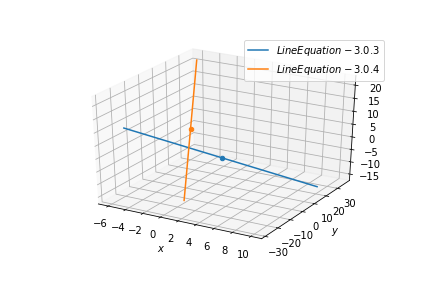
\includegraphics[width=\columnwidth]{./solutions/line_plane/74/codes/figs/Line_interest_1.png}
	\caption{Graph for equations \ref{eq:solutions/line_plane/74/codes7}}
	\label{fig:solutions/line_plane/74/codesline_equation_1}
\end{figure}


	\item 
	\begin{align}\label{eq:solutions/line_plane/74/codes12}
		\frac{x}{2} = \frac{y}{2} &= \frac{z}{1}, 
	\end{align}
	\begin{align}\label{eq:solutions/line_plane/74/codes13}
		\frac{x-5}{4} = \frac{y-2}{1} &= \frac{z-3}{8} 
	\end{align}



The above symmetric equations \ref{eq:solutions/line_plane/74/codes12}, \ref{eq:solutions/line_plane/74/codes13} can be represented in the vector form as 
\begin{align}\label{eq:solutions/line_plane/74/codes14}
	\quad \vec{r_1} &= \myvec{0\\0\\0} + \lambda_1\myvec{2\\2\\1}
	\\
	\quad \vec{r_2} &= \myvec{5\\2\\3} + \lambda_2\myvec{4\\1\\8}
\end{align}

As we have to find the angle between the vectors, we will only be taking the direction vectors into consideration. The direction vectors are $\vec{u}$ = $\myvec{2\\2\\1}$ and $\vec{v}$ = $\myvec{4\\1\\8}$. We can find the corresponding magnitude values

\begin{align}\label{eq:solutions/line_plane/74/codes16}
	\norm{\vec{u}} =\sqrt{2^{2}+2^{2}+1^{2}} =\sqrt{9}
\end{align}
\begin{align}\label{eq:solutions/line_plane/74/codes17}
	\norm{\vec{v}} =\sqrt{4^{2}+1^{2}+8^{2}} =\sqrt{81}
\end{align}

Using \ref{eq:solutions/line_plane/74/codes4}, \ref{eq:solutions/line_plane/74/codes16}, \ref{eq:solutions/line_plane/74/codes17} we get
\begin{align}
	\theta = \cos ^{-1}\frac{\myvec{2\\2\\1}^{T}\myvec{4\\1\\8}}{(\sqrt{9})(\sqrt{81})} 
	\\
	\theta = \cos ^{-1}\frac{18}{27.00}
	\\
	\theta = \cos ^{-1} (0.667)
	\\
	\theta = 48.189\degree
\end{align}

Therefore, the angle between the two lines is $48.189\degree$. See Fig. \ref{fig:solutions/line_plane/74/codesline_equation_2}


\begin{figure}
	\centering
	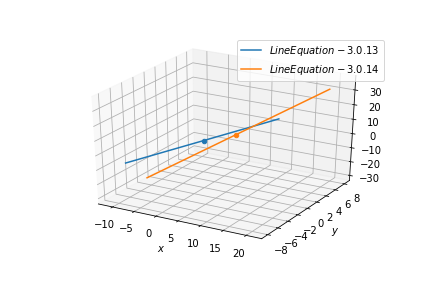
\includegraphics[width=\columnwidth]{./solutions/line_plane/74/codes/figs/Line_interest_2.png}
	\caption{Graph for equations \ref{eq:solutions/line_plane/74/codes14}}
	\label{fig:solutions/line_plane/74/codesline_equation_2}
\end{figure}
\end{enumerate}

    

%
\item Find the zero of the polynomial in each of the following cases: 
\begin{enumerate}
\item $p(x) = x + 5 $
\item $p(x) = x – 5$
\item $p(x) = 2x + 5$
\item $p(x) = 3x – 2$
 \item $p(x) = 3x$
 \item $p(x) = ax, a \ne 0$
\item $p(x) = cx + d, c \ne 0, c, d$ are real numbers.
\end{enumerate}
\solution 
From theory, we understand that using dot product we can find the angle between the lines 
\begin{enumerate}
	\item 
	\begin{align}\label{eq:solutions/line_plane/74/codes:5}
		\frac{x-2}{2} = \frac{y-1}{5} &= \frac{z+3}{-3}, 
	\end{align}
	\begin{align}\label{eq:solutions/line_plane/74/codes:6}
		\frac{x+2}{-1} = \frac{y-4}{8} &= \frac{z-5}{4} 
	\end{align}


The above symmetric equations \ref{eq:solutions/line_plane/74/codes:5}, \ref{eq:solutions/line_plane/74/codes:6} can be represented in the vector form as 
\begin{align}\label{eq:solutions/line_plane/74/codes7}
	\quad \vec{r_1} &= \myvec{2\\1\\-3} + \lambda_1\myvec{2\\5\\-3}
	\\
	\quad \vec{r_2} &= \myvec{-2\\4\\5} + \lambda_2\myvec{-1\\8\\4}
\end{align}

As we have to find the angle between the vectors, we will only be taking the direction vectors into consideration. The direction vectors are $\vec{u}$ = $\myvec{2\\5\\-3}$ and $\vec{v}$ = $\myvec{-1\\8\\4}$. We can find the corresponding magnitude values

\begin{align}\label{eq:solutions/line_plane/74/codes9}
	\norm{\vec{u}} =\sqrt{2^{2}+5^{2}+(-3)^{2}} =\sqrt{38}
\end{align}
\begin{align}\label{eq:solutions/line_plane/74/codes10}
	\norm{\vec{v}} =\sqrt{(-1)^{2}+8^{2}+4^{2}} =\sqrt{81}
\end{align}

Using \ref{eq:solutions/line_plane/74/codes4}, \ref{eq:solutions/line_plane/74/codes9}, \ref{eq:solutions/line_plane/74/codes10} we get
\begin{align}
	\theta = \cos ^{-1}\frac{\myvec{2\\5\\-3}^{T}\myvec{-1\\8\\4}}{(\sqrt{38})(\sqrt{81})} 
	\\
	\theta = \cos ^{-1}\frac{26}{55.4797}
	\\
	\theta = \cos ^{-1} (0.4686)
	\\
	\theta = 62.053\degree
\end{align}

Therefore, the angle between the two lines is $62.053\degree$.See Fig. \ref{fig:solutions/line_plane/74/codesline_equation_1}

\begin{figure}
	\centering
	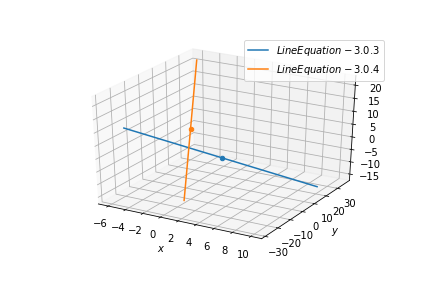
\includegraphics[width=\columnwidth]{./solutions/line_plane/74/codes/figs/Line_interest_1.png}
	\caption{Graph for equations \ref{eq:solutions/line_plane/74/codes7}}
	\label{fig:solutions/line_plane/74/codesline_equation_1}
\end{figure}


	\item 
	\begin{align}\label{eq:solutions/line_plane/74/codes12}
		\frac{x}{2} = \frac{y}{2} &= \frac{z}{1}, 
	\end{align}
	\begin{align}\label{eq:solutions/line_plane/74/codes13}
		\frac{x-5}{4} = \frac{y-2}{1} &= \frac{z-3}{8} 
	\end{align}



The above symmetric equations \ref{eq:solutions/line_plane/74/codes12}, \ref{eq:solutions/line_plane/74/codes13} can be represented in the vector form as 
\begin{align}\label{eq:solutions/line_plane/74/codes14}
	\quad \vec{r_1} &= \myvec{0\\0\\0} + \lambda_1\myvec{2\\2\\1}
	\\
	\quad \vec{r_2} &= \myvec{5\\2\\3} + \lambda_2\myvec{4\\1\\8}
\end{align}

As we have to find the angle between the vectors, we will only be taking the direction vectors into consideration. The direction vectors are $\vec{u}$ = $\myvec{2\\2\\1}$ and $\vec{v}$ = $\myvec{4\\1\\8}$. We can find the corresponding magnitude values

\begin{align}\label{eq:solutions/line_plane/74/codes16}
	\norm{\vec{u}} =\sqrt{2^{2}+2^{2}+1^{2}} =\sqrt{9}
\end{align}
\begin{align}\label{eq:solutions/line_plane/74/codes17}
	\norm{\vec{v}} =\sqrt{4^{2}+1^{2}+8^{2}} =\sqrt{81}
\end{align}

Using \ref{eq:solutions/line_plane/74/codes4}, \ref{eq:solutions/line_plane/74/codes16}, \ref{eq:solutions/line_plane/74/codes17} we get
\begin{align}
	\theta = \cos ^{-1}\frac{\myvec{2\\2\\1}^{T}\myvec{4\\1\\8}}{(\sqrt{9})(\sqrt{81})} 
	\\
	\theta = \cos ^{-1}\frac{18}{27.00}
	\\
	\theta = \cos ^{-1} (0.667)
	\\
	\theta = 48.189\degree
\end{align}

Therefore, the angle between the two lines is $48.189\degree$. See Fig. \ref{fig:solutions/line_plane/74/codesline_equation_2}


\begin{figure}
	\centering
	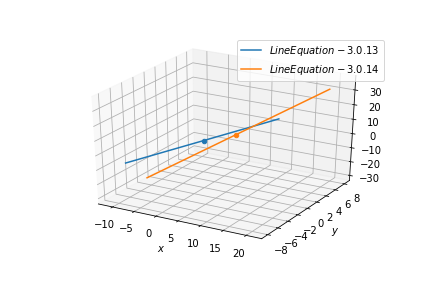
\includegraphics[width=\columnwidth]{./solutions/line_plane/74/codes/figs/Line_interest_2.png}
	\caption{Graph for equations \ref{eq:solutions/line_plane/74/codes14}}
	\label{fig:solutions/line_plane/74/codesline_equation_2}
\end{figure}
\end{enumerate}

    

\item Find two solutions for each of the following equations: 
\begin{enumerate}
\item $\myvec{4 & 3}\vec{x} = 12$
\item $\myvec{ 2 & 5}\vec{x}  = 0 $
\item $\myvec{ 0 & 3}\vec{x}  = 4$
\end{enumerate}
\solution 
From theory, we understand that using dot product we can find the angle between the lines 
\begin{enumerate}
	\item 
	\begin{align}\label{eq:solutions/line_plane/74/codes:5}
		\frac{x-2}{2} = \frac{y-1}{5} &= \frac{z+3}{-3}, 
	\end{align}
	\begin{align}\label{eq:solutions/line_plane/74/codes:6}
		\frac{x+2}{-1} = \frac{y-4}{8} &= \frac{z-5}{4} 
	\end{align}


The above symmetric equations \ref{eq:solutions/line_plane/74/codes:5}, \ref{eq:solutions/line_plane/74/codes:6} can be represented in the vector form as 
\begin{align}\label{eq:solutions/line_plane/74/codes7}
	\quad \vec{r_1} &= \myvec{2\\1\\-3} + \lambda_1\myvec{2\\5\\-3}
	\\
	\quad \vec{r_2} &= \myvec{-2\\4\\5} + \lambda_2\myvec{-1\\8\\4}
\end{align}

As we have to find the angle between the vectors, we will only be taking the direction vectors into consideration. The direction vectors are $\vec{u}$ = $\myvec{2\\5\\-3}$ and $\vec{v}$ = $\myvec{-1\\8\\4}$. We can find the corresponding magnitude values

\begin{align}\label{eq:solutions/line_plane/74/codes9}
	\norm{\vec{u}} =\sqrt{2^{2}+5^{2}+(-3)^{2}} =\sqrt{38}
\end{align}
\begin{align}\label{eq:solutions/line_plane/74/codes10}
	\norm{\vec{v}} =\sqrt{(-1)^{2}+8^{2}+4^{2}} =\sqrt{81}
\end{align}

Using \ref{eq:solutions/line_plane/74/codes4}, \ref{eq:solutions/line_plane/74/codes9}, \ref{eq:solutions/line_plane/74/codes10} we get
\begin{align}
	\theta = \cos ^{-1}\frac{\myvec{2\\5\\-3}^{T}\myvec{-1\\8\\4}}{(\sqrt{38})(\sqrt{81})} 
	\\
	\theta = \cos ^{-1}\frac{26}{55.4797}
	\\
	\theta = \cos ^{-1} (0.4686)
	\\
	\theta = 62.053\degree
\end{align}

Therefore, the angle between the two lines is $62.053\degree$.See Fig. \ref{fig:solutions/line_plane/74/codesline_equation_1}

\begin{figure}
	\centering
	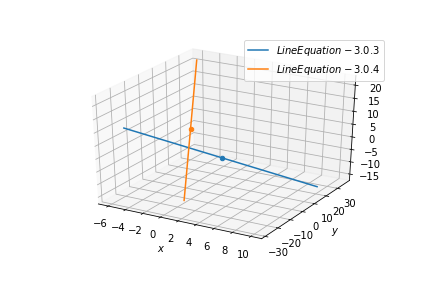
\includegraphics[width=\columnwidth]{./solutions/line_plane/74/codes/figs/Line_interest_1.png}
	\caption{Graph for equations \ref{eq:solutions/line_plane/74/codes7}}
	\label{fig:solutions/line_plane/74/codesline_equation_1}
\end{figure}


	\item 
	\begin{align}\label{eq:solutions/line_plane/74/codes12}
		\frac{x}{2} = \frac{y}{2} &= \frac{z}{1}, 
	\end{align}
	\begin{align}\label{eq:solutions/line_plane/74/codes13}
		\frac{x-5}{4} = \frac{y-2}{1} &= \frac{z-3}{8} 
	\end{align}



The above symmetric equations \ref{eq:solutions/line_plane/74/codes12}, \ref{eq:solutions/line_plane/74/codes13} can be represented in the vector form as 
\begin{align}\label{eq:solutions/line_plane/74/codes14}
	\quad \vec{r_1} &= \myvec{0\\0\\0} + \lambda_1\myvec{2\\2\\1}
	\\
	\quad \vec{r_2} &= \myvec{5\\2\\3} + \lambda_2\myvec{4\\1\\8}
\end{align}

As we have to find the angle between the vectors, we will only be taking the direction vectors into consideration. The direction vectors are $\vec{u}$ = $\myvec{2\\2\\1}$ and $\vec{v}$ = $\myvec{4\\1\\8}$. We can find the corresponding magnitude values

\begin{align}\label{eq:solutions/line_plane/74/codes16}
	\norm{\vec{u}} =\sqrt{2^{2}+2^{2}+1^{2}} =\sqrt{9}
\end{align}
\begin{align}\label{eq:solutions/line_plane/74/codes17}
	\norm{\vec{v}} =\sqrt{4^{2}+1^{2}+8^{2}} =\sqrt{81}
\end{align}

Using \ref{eq:solutions/line_plane/74/codes4}, \ref{eq:solutions/line_plane/74/codes16}, \ref{eq:solutions/line_plane/74/codes17} we get
\begin{align}
	\theta = \cos ^{-1}\frac{\myvec{2\\2\\1}^{T}\myvec{4\\1\\8}}{(\sqrt{9})(\sqrt{81})} 
	\\
	\theta = \cos ^{-1}\frac{18}{27.00}
	\\
	\theta = \cos ^{-1} (0.667)
	\\
	\theta = 48.189\degree
\end{align}

Therefore, the angle between the two lines is $48.189\degree$. See Fig. \ref{fig:solutions/line_plane/74/codesline_equation_2}


\begin{figure}
	\centering
	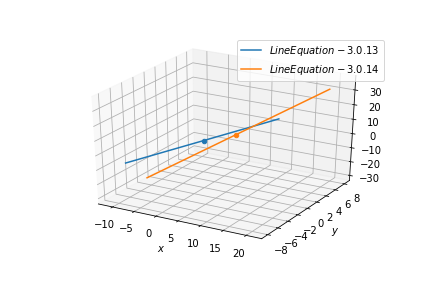
\includegraphics[width=\columnwidth]{./solutions/line_plane/74/codes/figs/Line_interest_2.png}
	\caption{Graph for equations \ref{eq:solutions/line_plane/74/codes14}}
	\label{fig:solutions/line_plane/74/codesline_equation_2}
\end{figure}
\end{enumerate}

    


\item Sketch the following lines
%
\begin{enumerate}[itemsep=2pt]
%\begin{multicols}{2}
\item
$
\myvec{2 & 3 }\vec{x}=9.35
$
\item
$
\myvec{1 & -\frac{1}{5} }\vec{x}=10
$
\item
$
\myvec{-2 & 3 }\vec{x}=6
$
\item
$
\myvec{1 & -3 }\vec{x}=0
$
\item
$
\myvec{2 & 5 }\vec{x}=0
$
\item
$
\myvec{3 & 0 }\vec{x}=-2
$
\item
$
\myvec{0 & 1 }\vec{x}=2
$
\item
$
\myvec{2 & 0 }\vec{x}=5
$
%\end{multicols}
\end{enumerate}
%
\solution 
From theory, we understand that using dot product we can find the angle between the lines 
\begin{enumerate}
	\item 
	\begin{align}\label{eq:solutions/line_plane/74/codes:5}
		\frac{x-2}{2} = \frac{y-1}{5} &= \frac{z+3}{-3}, 
	\end{align}
	\begin{align}\label{eq:solutions/line_plane/74/codes:6}
		\frac{x+2}{-1} = \frac{y-4}{8} &= \frac{z-5}{4} 
	\end{align}


The above symmetric equations \ref{eq:solutions/line_plane/74/codes:5}, \ref{eq:solutions/line_plane/74/codes:6} can be represented in the vector form as 
\begin{align}\label{eq:solutions/line_plane/74/codes7}
	\quad \vec{r_1} &= \myvec{2\\1\\-3} + \lambda_1\myvec{2\\5\\-3}
	\\
	\quad \vec{r_2} &= \myvec{-2\\4\\5} + \lambda_2\myvec{-1\\8\\4}
\end{align}

As we have to find the angle between the vectors, we will only be taking the direction vectors into consideration. The direction vectors are $\vec{u}$ = $\myvec{2\\5\\-3}$ and $\vec{v}$ = $\myvec{-1\\8\\4}$. We can find the corresponding magnitude values

\begin{align}\label{eq:solutions/line_plane/74/codes9}
	\norm{\vec{u}} =\sqrt{2^{2}+5^{2}+(-3)^{2}} =\sqrt{38}
\end{align}
\begin{align}\label{eq:solutions/line_plane/74/codes10}
	\norm{\vec{v}} =\sqrt{(-1)^{2}+8^{2}+4^{2}} =\sqrt{81}
\end{align}

Using \ref{eq:solutions/line_plane/74/codes4}, \ref{eq:solutions/line_plane/74/codes9}, \ref{eq:solutions/line_plane/74/codes10} we get
\begin{align}
	\theta = \cos ^{-1}\frac{\myvec{2\\5\\-3}^{T}\myvec{-1\\8\\4}}{(\sqrt{38})(\sqrt{81})} 
	\\
	\theta = \cos ^{-1}\frac{26}{55.4797}
	\\
	\theta = \cos ^{-1} (0.4686)
	\\
	\theta = 62.053\degree
\end{align}

Therefore, the angle between the two lines is $62.053\degree$.See Fig. \ref{fig:solutions/line_plane/74/codesline_equation_1}

\begin{figure}
	\centering
	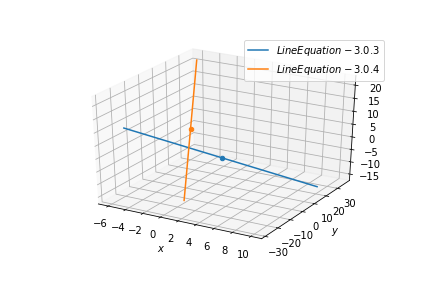
\includegraphics[width=\columnwidth]{./solutions/line_plane/74/codes/figs/Line_interest_1.png}
	\caption{Graph for equations \ref{eq:solutions/line_plane/74/codes7}}
	\label{fig:solutions/line_plane/74/codesline_equation_1}
\end{figure}


	\item 
	\begin{align}\label{eq:solutions/line_plane/74/codes12}
		\frac{x}{2} = \frac{y}{2} &= \frac{z}{1}, 
	\end{align}
	\begin{align}\label{eq:solutions/line_plane/74/codes13}
		\frac{x-5}{4} = \frac{y-2}{1} &= \frac{z-3}{8} 
	\end{align}



The above symmetric equations \ref{eq:solutions/line_plane/74/codes12}, \ref{eq:solutions/line_plane/74/codes13} can be represented in the vector form as 
\begin{align}\label{eq:solutions/line_plane/74/codes14}
	\quad \vec{r_1} &= \myvec{0\\0\\0} + \lambda_1\myvec{2\\2\\1}
	\\
	\quad \vec{r_2} &= \myvec{5\\2\\3} + \lambda_2\myvec{4\\1\\8}
\end{align}

As we have to find the angle between the vectors, we will only be taking the direction vectors into consideration. The direction vectors are $\vec{u}$ = $\myvec{2\\2\\1}$ and $\vec{v}$ = $\myvec{4\\1\\8}$. We can find the corresponding magnitude values

\begin{align}\label{eq:solutions/line_plane/74/codes16}
	\norm{\vec{u}} =\sqrt{2^{2}+2^{2}+1^{2}} =\sqrt{9}
\end{align}
\begin{align}\label{eq:solutions/line_plane/74/codes17}
	\norm{\vec{v}} =\sqrt{4^{2}+1^{2}+8^{2}} =\sqrt{81}
\end{align}

Using \ref{eq:solutions/line_plane/74/codes4}, \ref{eq:solutions/line_plane/74/codes16}, \ref{eq:solutions/line_plane/74/codes17} we get
\begin{align}
	\theta = \cos ^{-1}\frac{\myvec{2\\2\\1}^{T}\myvec{4\\1\\8}}{(\sqrt{9})(\sqrt{81})} 
	\\
	\theta = \cos ^{-1}\frac{18}{27.00}
	\\
	\theta = \cos ^{-1} (0.667)
	\\
	\theta = 48.189\degree
\end{align}

Therefore, the angle between the two lines is $48.189\degree$. See Fig. \ref{fig:solutions/line_plane/74/codesline_equation_2}


\begin{figure}
	\centering
	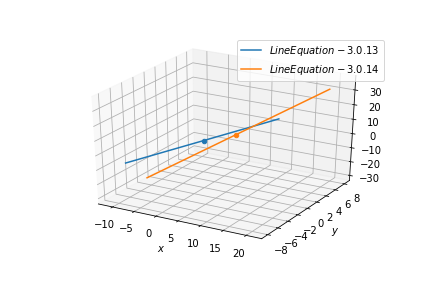
\includegraphics[width=\columnwidth]{./solutions/line_plane/74/codes/figs/Line_interest_2.png}
	\caption{Graph for equations \ref{eq:solutions/line_plane/74/codes14}}
	\label{fig:solutions/line_plane/74/codesline_equation_2}
\end{figure}
\end{enumerate}

    

%
\item Draw the graphs of the following equations
\begin{enumerate}[itemsep=2pt]
\begin{multicols}{2}
\item $\myvec{1 & 1}\vec{x} = 0$
\item $\myvec{ 2 & -1}\vec{x}  = 0 $
\item $\myvec{ 1 & -1}\vec{x}  = 0$
\item $\myvec{ 2 & -1}\vec{x}  = -1$
\item $\myvec{ 2 & -1}\vec{x}  = 4$
\item $\myvec{ 1& -1}\vec{x}  = 4$
\end{multicols}
\end{enumerate}
\solution 
	The following python codes draw the graphs which are represented in Fig.\ref{fig:3.7.5_qelevena} and Fig.\ref{fig:3.7.5_qelevenb}.
	\begin{lstlisting}
	./solutions/5/codes/lines/q11a.py
	./solutions/5/codes/lines/q11b.py
	\end{lstlisting}
	\solution
	\begin{figure}[!ht]
	\centering
	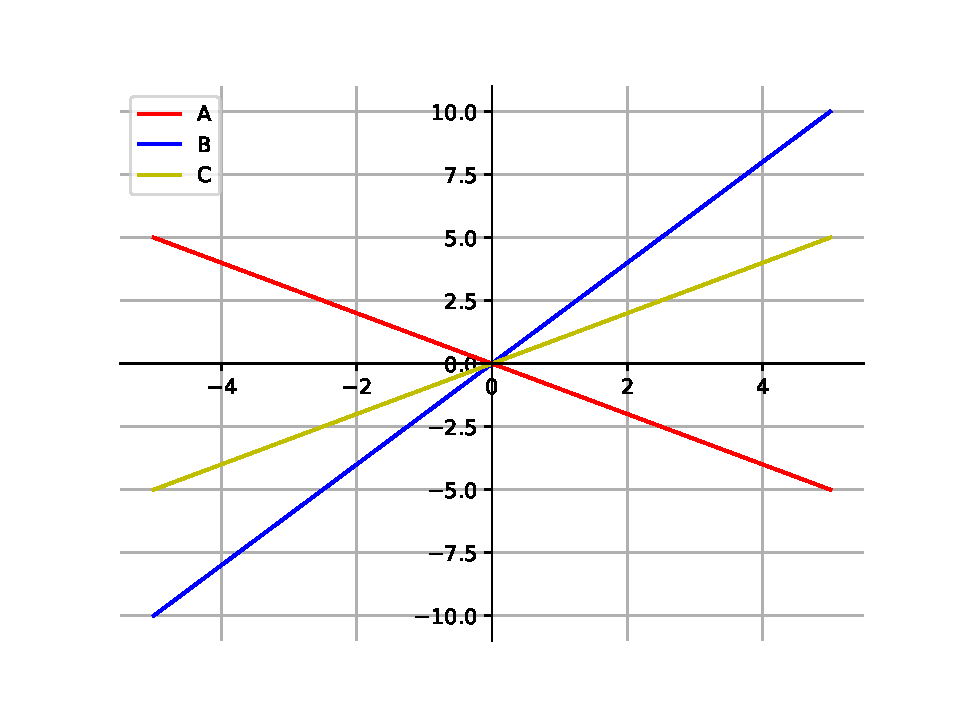
\includegraphics[width=\columnwidth]{./solutions/5/figs/lines/q11a.eps}
	\caption{}
	\label{fig:3.7.5_qelevena}	
	\end{figure}
	\begin{figure}[!ht]
	\centering
	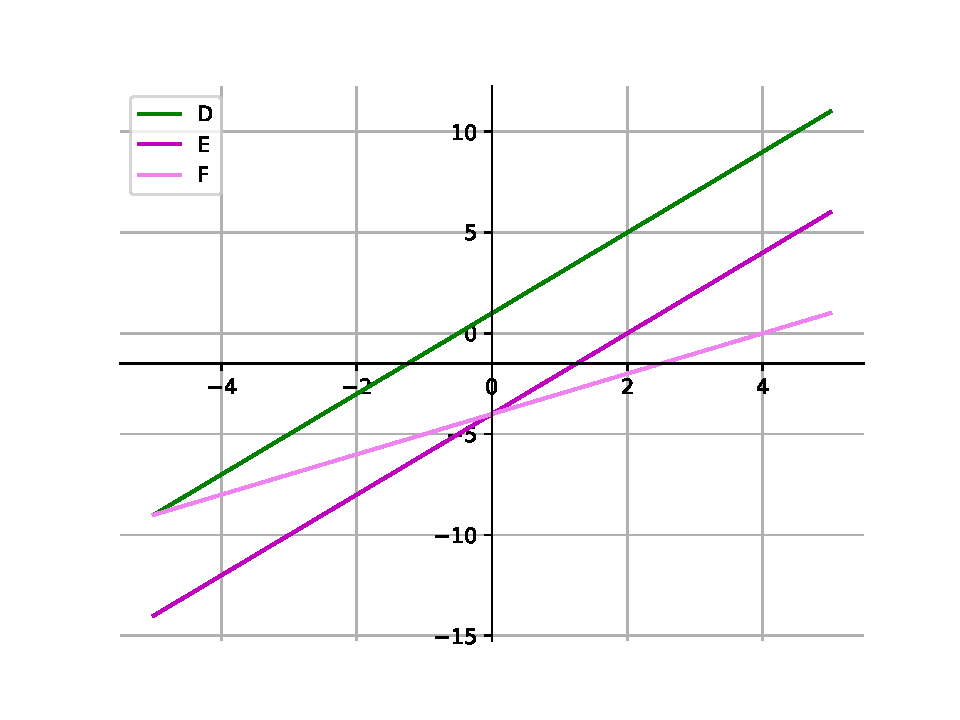
\includegraphics[width=\columnwidth]{./solutions/5/figs/lines/q11b.eps}
	\caption{}
	\label{fig:3.7.5_qelevenb}	
	\end{figure}
	

%
\item Write four solutions for each of the following equations
\begin{enumerate}
\item $\myvec{2 & 1}\vec{x} = 7$
\item $\myvec{ \pi & 1}\vec{x}  = 9 $
\item $\myvec{ 1 & -4}\vec{x}  = 0$
\end{enumerate}
\solution 
From theory, we understand that using dot product we can find the angle between the lines 
\begin{enumerate}
	\item 
	\begin{align}\label{eq:solutions/line_plane/74/codes:5}
		\frac{x-2}{2} = \frac{y-1}{5} &= \frac{z+3}{-3}, 
	\end{align}
	\begin{align}\label{eq:solutions/line_plane/74/codes:6}
		\frac{x+2}{-1} = \frac{y-4}{8} &= \frac{z-5}{4} 
	\end{align}


The above symmetric equations \ref{eq:solutions/line_plane/74/codes:5}, \ref{eq:solutions/line_plane/74/codes:6} can be represented in the vector form as 
\begin{align}\label{eq:solutions/line_plane/74/codes7}
	\quad \vec{r_1} &= \myvec{2\\1\\-3} + \lambda_1\myvec{2\\5\\-3}
	\\
	\quad \vec{r_2} &= \myvec{-2\\4\\5} + \lambda_2\myvec{-1\\8\\4}
\end{align}

As we have to find the angle between the vectors, we will only be taking the direction vectors into consideration. The direction vectors are $\vec{u}$ = $\myvec{2\\5\\-3}$ and $\vec{v}$ = $\myvec{-1\\8\\4}$. We can find the corresponding magnitude values

\begin{align}\label{eq:solutions/line_plane/74/codes9}
	\norm{\vec{u}} =\sqrt{2^{2}+5^{2}+(-3)^{2}} =\sqrt{38}
\end{align}
\begin{align}\label{eq:solutions/line_plane/74/codes10}
	\norm{\vec{v}} =\sqrt{(-1)^{2}+8^{2}+4^{2}} =\sqrt{81}
\end{align}

Using \ref{eq:solutions/line_plane/74/codes4}, \ref{eq:solutions/line_plane/74/codes9}, \ref{eq:solutions/line_plane/74/codes10} we get
\begin{align}
	\theta = \cos ^{-1}\frac{\myvec{2\\5\\-3}^{T}\myvec{-1\\8\\4}}{(\sqrt{38})(\sqrt{81})} 
	\\
	\theta = \cos ^{-1}\frac{26}{55.4797}
	\\
	\theta = \cos ^{-1} (0.4686)
	\\
	\theta = 62.053\degree
\end{align}

Therefore, the angle between the two lines is $62.053\degree$.See Fig. \ref{fig:solutions/line_plane/74/codesline_equation_1}

\begin{figure}
	\centering
	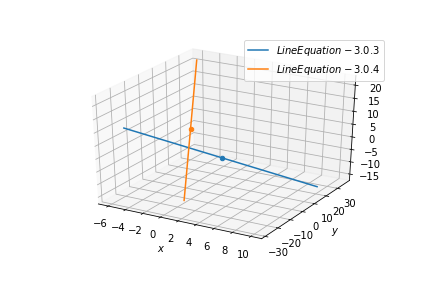
\includegraphics[width=\columnwidth]{./solutions/line_plane/74/codes/figs/Line_interest_1.png}
	\caption{Graph for equations \ref{eq:solutions/line_plane/74/codes7}}
	\label{fig:solutions/line_plane/74/codesline_equation_1}
\end{figure}


	\item 
	\begin{align}\label{eq:solutions/line_plane/74/codes12}
		\frac{x}{2} = \frac{y}{2} &= \frac{z}{1}, 
	\end{align}
	\begin{align}\label{eq:solutions/line_plane/74/codes13}
		\frac{x-5}{4} = \frac{y-2}{1} &= \frac{z-3}{8} 
	\end{align}



The above symmetric equations \ref{eq:solutions/line_plane/74/codes12}, \ref{eq:solutions/line_plane/74/codes13} can be represented in the vector form as 
\begin{align}\label{eq:solutions/line_plane/74/codes14}
	\quad \vec{r_1} &= \myvec{0\\0\\0} + \lambda_1\myvec{2\\2\\1}
	\\
	\quad \vec{r_2} &= \myvec{5\\2\\3} + \lambda_2\myvec{4\\1\\8}
\end{align}

As we have to find the angle between the vectors, we will only be taking the direction vectors into consideration. The direction vectors are $\vec{u}$ = $\myvec{2\\2\\1}$ and $\vec{v}$ = $\myvec{4\\1\\8}$. We can find the corresponding magnitude values

\begin{align}\label{eq:solutions/line_plane/74/codes16}
	\norm{\vec{u}} =\sqrt{2^{2}+2^{2}+1^{2}} =\sqrt{9}
\end{align}
\begin{align}\label{eq:solutions/line_plane/74/codes17}
	\norm{\vec{v}} =\sqrt{4^{2}+1^{2}+8^{2}} =\sqrt{81}
\end{align}

Using \ref{eq:solutions/line_plane/74/codes4}, \ref{eq:solutions/line_plane/74/codes16}, \ref{eq:solutions/line_plane/74/codes17} we get
\begin{align}
	\theta = \cos ^{-1}\frac{\myvec{2\\2\\1}^{T}\myvec{4\\1\\8}}{(\sqrt{9})(\sqrt{81})} 
	\\
	\theta = \cos ^{-1}\frac{18}{27.00}
	\\
	\theta = \cos ^{-1} (0.667)
	\\
	\theta = 48.189\degree
\end{align}

Therefore, the angle between the two lines is $48.189\degree$. See Fig. \ref{fig:solutions/line_plane/74/codesline_equation_2}


\begin{figure}
	\centering
	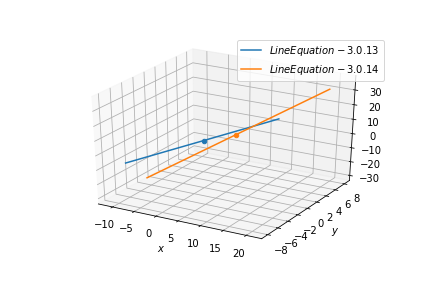
\includegraphics[width=\columnwidth]{./solutions/line_plane/74/codes/figs/Line_interest_2.png}
	\caption{Graph for equations \ref{eq:solutions/line_plane/74/codes14}}
	\label{fig:solutions/line_plane/74/codesline_equation_2}
\end{figure}
\end{enumerate}

    

\item Find $m$ if 
\begin{align}
\begin{split}
\myvec{2 & 3 }\vec{x}&=11
\\
\myvec{2 & -4 }\vec{x}&=-24
\\
\myvec{m & -1 }\vec{x}&=-3
\\
\end{split}
\end{align}
%
\solution 
From theory, we understand that using dot product we can find the angle between the lines 
\begin{enumerate}
	\item 
	\begin{align}\label{eq:solutions/line_plane/74/codes:5}
		\frac{x-2}{2} = \frac{y-1}{5} &= \frac{z+3}{-3}, 
	\end{align}
	\begin{align}\label{eq:solutions/line_plane/74/codes:6}
		\frac{x+2}{-1} = \frac{y-4}{8} &= \frac{z-5}{4} 
	\end{align}


The above symmetric equations \ref{eq:solutions/line_plane/74/codes:5}, \ref{eq:solutions/line_plane/74/codes:6} can be represented in the vector form as 
\begin{align}\label{eq:solutions/line_plane/74/codes7}
	\quad \vec{r_1} &= \myvec{2\\1\\-3} + \lambda_1\myvec{2\\5\\-3}
	\\
	\quad \vec{r_2} &= \myvec{-2\\4\\5} + \lambda_2\myvec{-1\\8\\4}
\end{align}

As we have to find the angle between the vectors, we will only be taking the direction vectors into consideration. The direction vectors are $\vec{u}$ = $\myvec{2\\5\\-3}$ and $\vec{v}$ = $\myvec{-1\\8\\4}$. We can find the corresponding magnitude values

\begin{align}\label{eq:solutions/line_plane/74/codes9}
	\norm{\vec{u}} =\sqrt{2^{2}+5^{2}+(-3)^{2}} =\sqrt{38}
\end{align}
\begin{align}\label{eq:solutions/line_plane/74/codes10}
	\norm{\vec{v}} =\sqrt{(-1)^{2}+8^{2}+4^{2}} =\sqrt{81}
\end{align}

Using \ref{eq:solutions/line_plane/74/codes4}, \ref{eq:solutions/line_plane/74/codes9}, \ref{eq:solutions/line_plane/74/codes10} we get
\begin{align}
	\theta = \cos ^{-1}\frac{\myvec{2\\5\\-3}^{T}\myvec{-1\\8\\4}}{(\sqrt{38})(\sqrt{81})} 
	\\
	\theta = \cos ^{-1}\frac{26}{55.4797}
	\\
	\theta = \cos ^{-1} (0.4686)
	\\
	\theta = 62.053\degree
\end{align}

Therefore, the angle between the two lines is $62.053\degree$.See Fig. \ref{fig:solutions/line_plane/74/codesline_equation_1}

\begin{figure}
	\centering
	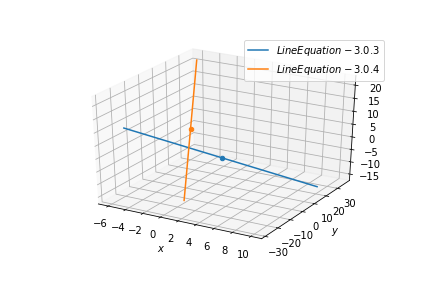
\includegraphics[width=\columnwidth]{./solutions/line_plane/74/codes/figs/Line_interest_1.png}
	\caption{Graph for equations \ref{eq:solutions/line_plane/74/codes7}}
	\label{fig:solutions/line_plane/74/codesline_equation_1}
\end{figure}


	\item 
	\begin{align}\label{eq:solutions/line_plane/74/codes12}
		\frac{x}{2} = \frac{y}{2} &= \frac{z}{1}, 
	\end{align}
	\begin{align}\label{eq:solutions/line_plane/74/codes13}
		\frac{x-5}{4} = \frac{y-2}{1} &= \frac{z-3}{8} 
	\end{align}



The above symmetric equations \ref{eq:solutions/line_plane/74/codes12}, \ref{eq:solutions/line_plane/74/codes13} can be represented in the vector form as 
\begin{align}\label{eq:solutions/line_plane/74/codes14}
	\quad \vec{r_1} &= \myvec{0\\0\\0} + \lambda_1\myvec{2\\2\\1}
	\\
	\quad \vec{r_2} &= \myvec{5\\2\\3} + \lambda_2\myvec{4\\1\\8}
\end{align}

As we have to find the angle between the vectors, we will only be taking the direction vectors into consideration. The direction vectors are $\vec{u}$ = $\myvec{2\\2\\1}$ and $\vec{v}$ = $\myvec{4\\1\\8}$. We can find the corresponding magnitude values

\begin{align}\label{eq:solutions/line_plane/74/codes16}
	\norm{\vec{u}} =\sqrt{2^{2}+2^{2}+1^{2}} =\sqrt{9}
\end{align}
\begin{align}\label{eq:solutions/line_plane/74/codes17}
	\norm{\vec{v}} =\sqrt{4^{2}+1^{2}+8^{2}} =\sqrt{81}
\end{align}

Using \ref{eq:solutions/line_plane/74/codes4}, \ref{eq:solutions/line_plane/74/codes16}, \ref{eq:solutions/line_plane/74/codes17} we get
\begin{align}
	\theta = \cos ^{-1}\frac{\myvec{2\\2\\1}^{T}\myvec{4\\1\\8}}{(\sqrt{9})(\sqrt{81})} 
	\\
	\theta = \cos ^{-1}\frac{18}{27.00}
	\\
	\theta = \cos ^{-1} (0.667)
	\\
	\theta = 48.189\degree
\end{align}

Therefore, the angle between the two lines is $48.189\degree$. See Fig. \ref{fig:solutions/line_plane/74/codesline_equation_2}


\begin{figure}
	\centering
	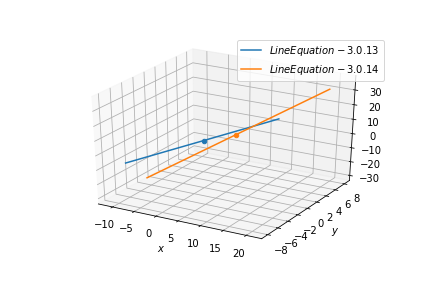
\includegraphics[width=\columnwidth]{./solutions/line_plane/74/codes/figs/Line_interest_2.png}
	\caption{Graph for equations \ref{eq:solutions/line_plane/74/codes14}}
	\label{fig:solutions/line_plane/74/codesline_equation_2}
\end{figure}
\end{enumerate}

    

\item Solve the following
%
\begin{enumerate}[itemsep=2pt]
\begin{multicols}{2}
\item
\begin{align}
\begin{split}
\myvec{1 & 1 }\vec{x}&=5
\\
\myvec{2 & -3 }\vec{x}&=4
\end{split}
\end{align}
\item
\begin{align}
\begin{split}
\myvec{3 & 4 }\vec{x}&=10
\\
\myvec{2 & -2 }\vec{x}&=2
\end{split}
\end{align}
\item
\begin{align}
\begin{split}
\myvec{3 & -5 }\vec{x}&=4
\\
\myvec{9 & -2 }\vec{x}&=7
\end{split}
\end{align}
\begin{align}
\begin{split}
\myvec{\frac{1}{2} & \frac{2}{3} }\vec{x}&=-1
\\
\myvec{{1} & -\frac{1}{3} }\vec{x}&=3
\end{split}
\end{align}
\end{multicols}
\end{enumerate}
%
\solution 
From theory, we understand that using dot product we can find the angle between the lines 
\begin{enumerate}
	\item 
	\begin{align}\label{eq:solutions/line_plane/74/codes:5}
		\frac{x-2}{2} = \frac{y-1}{5} &= \frac{z+3}{-3}, 
	\end{align}
	\begin{align}\label{eq:solutions/line_plane/74/codes:6}
		\frac{x+2}{-1} = \frac{y-4}{8} &= \frac{z-5}{4} 
	\end{align}


The above symmetric equations \ref{eq:solutions/line_plane/74/codes:5}, \ref{eq:solutions/line_plane/74/codes:6} can be represented in the vector form as 
\begin{align}\label{eq:solutions/line_plane/74/codes7}
	\quad \vec{r_1} &= \myvec{2\\1\\-3} + \lambda_1\myvec{2\\5\\-3}
	\\
	\quad \vec{r_2} &= \myvec{-2\\4\\5} + \lambda_2\myvec{-1\\8\\4}
\end{align}

As we have to find the angle between the vectors, we will only be taking the direction vectors into consideration. The direction vectors are $\vec{u}$ = $\myvec{2\\5\\-3}$ and $\vec{v}$ = $\myvec{-1\\8\\4}$. We can find the corresponding magnitude values

\begin{align}\label{eq:solutions/line_plane/74/codes9}
	\norm{\vec{u}} =\sqrt{2^{2}+5^{2}+(-3)^{2}} =\sqrt{38}
\end{align}
\begin{align}\label{eq:solutions/line_plane/74/codes10}
	\norm{\vec{v}} =\sqrt{(-1)^{2}+8^{2}+4^{2}} =\sqrt{81}
\end{align}

Using \ref{eq:solutions/line_plane/74/codes4}, \ref{eq:solutions/line_plane/74/codes9}, \ref{eq:solutions/line_plane/74/codes10} we get
\begin{align}
	\theta = \cos ^{-1}\frac{\myvec{2\\5\\-3}^{T}\myvec{-1\\8\\4}}{(\sqrt{38})(\sqrt{81})} 
	\\
	\theta = \cos ^{-1}\frac{26}{55.4797}
	\\
	\theta = \cos ^{-1} (0.4686)
	\\
	\theta = 62.053\degree
\end{align}

Therefore, the angle between the two lines is $62.053\degree$.See Fig. \ref{fig:solutions/line_plane/74/codesline_equation_1}

\begin{figure}
	\centering
	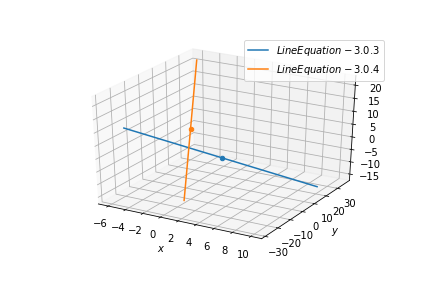
\includegraphics[width=\columnwidth]{./solutions/line_plane/74/codes/figs/Line_interest_1.png}
	\caption{Graph for equations \ref{eq:solutions/line_plane/74/codes7}}
	\label{fig:solutions/line_plane/74/codesline_equation_1}
\end{figure}


	\item 
	\begin{align}\label{eq:solutions/line_plane/74/codes12}
		\frac{x}{2} = \frac{y}{2} &= \frac{z}{1}, 
	\end{align}
	\begin{align}\label{eq:solutions/line_plane/74/codes13}
		\frac{x-5}{4} = \frac{y-2}{1} &= \frac{z-3}{8} 
	\end{align}



The above symmetric equations \ref{eq:solutions/line_plane/74/codes12}, \ref{eq:solutions/line_plane/74/codes13} can be represented in the vector form as 
\begin{align}\label{eq:solutions/line_plane/74/codes14}
	\quad \vec{r_1} &= \myvec{0\\0\\0} + \lambda_1\myvec{2\\2\\1}
	\\
	\quad \vec{r_2} &= \myvec{5\\2\\3} + \lambda_2\myvec{4\\1\\8}
\end{align}

As we have to find the angle between the vectors, we will only be taking the direction vectors into consideration. The direction vectors are $\vec{u}$ = $\myvec{2\\2\\1}$ and $\vec{v}$ = $\myvec{4\\1\\8}$. We can find the corresponding magnitude values

\begin{align}\label{eq:solutions/line_plane/74/codes16}
	\norm{\vec{u}} =\sqrt{2^{2}+2^{2}+1^{2}} =\sqrt{9}
\end{align}
\begin{align}\label{eq:solutions/line_plane/74/codes17}
	\norm{\vec{v}} =\sqrt{4^{2}+1^{2}+8^{2}} =\sqrt{81}
\end{align}

Using \ref{eq:solutions/line_plane/74/codes4}, \ref{eq:solutions/line_plane/74/codes16}, \ref{eq:solutions/line_plane/74/codes17} we get
\begin{align}
	\theta = \cos ^{-1}\frac{\myvec{2\\2\\1}^{T}\myvec{4\\1\\8}}{(\sqrt{9})(\sqrt{81})} 
	\\
	\theta = \cos ^{-1}\frac{18}{27.00}
	\\
	\theta = \cos ^{-1} (0.667)
	\\
	\theta = 48.189\degree
\end{align}

Therefore, the angle between the two lines is $48.189\degree$. See Fig. \ref{fig:solutions/line_plane/74/codesline_equation_2}


\begin{figure}
	\centering
	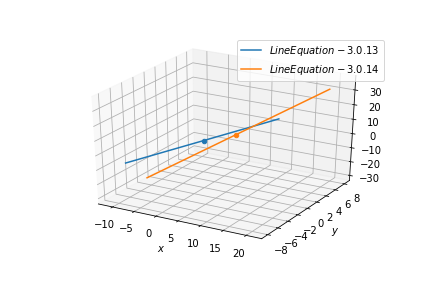
\includegraphics[width=\columnwidth]{./solutions/line_plane/74/codes/figs/Line_interest_2.png}
	\caption{Graph for equations \ref{eq:solutions/line_plane/74/codes14}}
	\label{fig:solutions/line_plane/74/codesline_equation_2}
\end{figure}
\end{enumerate}

    


\item For which values of $a$ and $b$ does the following pair of linear equations have an infinite number of solutions?
\begin{align}
\begin{split}
\myvec{2 & 3 }\vec{x}&=7
\\
\myvec{a-b & a+b }\vec{x}&=3a+b-2
\end{split}
\end{align}
\solution 
From theory, we understand that using dot product we can find the angle between the lines 
\begin{enumerate}
	\item 
	\begin{align}\label{eq:solutions/line_plane/74/codes:5}
		\frac{x-2}{2} = \frac{y-1}{5} &= \frac{z+3}{-3}, 
	\end{align}
	\begin{align}\label{eq:solutions/line_plane/74/codes:6}
		\frac{x+2}{-1} = \frac{y-4}{8} &= \frac{z-5}{4} 
	\end{align}


The above symmetric equations \ref{eq:solutions/line_plane/74/codes:5}, \ref{eq:solutions/line_plane/74/codes:6} can be represented in the vector form as 
\begin{align}\label{eq:solutions/line_plane/74/codes7}
	\quad \vec{r_1} &= \myvec{2\\1\\-3} + \lambda_1\myvec{2\\5\\-3}
	\\
	\quad \vec{r_2} &= \myvec{-2\\4\\5} + \lambda_2\myvec{-1\\8\\4}
\end{align}

As we have to find the angle between the vectors, we will only be taking the direction vectors into consideration. The direction vectors are $\vec{u}$ = $\myvec{2\\5\\-3}$ and $\vec{v}$ = $\myvec{-1\\8\\4}$. We can find the corresponding magnitude values

\begin{align}\label{eq:solutions/line_plane/74/codes9}
	\norm{\vec{u}} =\sqrt{2^{2}+5^{2}+(-3)^{2}} =\sqrt{38}
\end{align}
\begin{align}\label{eq:solutions/line_plane/74/codes10}
	\norm{\vec{v}} =\sqrt{(-1)^{2}+8^{2}+4^{2}} =\sqrt{81}
\end{align}

Using \ref{eq:solutions/line_plane/74/codes4}, \ref{eq:solutions/line_plane/74/codes9}, \ref{eq:solutions/line_plane/74/codes10} we get
\begin{align}
	\theta = \cos ^{-1}\frac{\myvec{2\\5\\-3}^{T}\myvec{-1\\8\\4}}{(\sqrt{38})(\sqrt{81})} 
	\\
	\theta = \cos ^{-1}\frac{26}{55.4797}
	\\
	\theta = \cos ^{-1} (0.4686)
	\\
	\theta = 62.053\degree
\end{align}

Therefore, the angle between the two lines is $62.053\degree$.See Fig. \ref{fig:solutions/line_plane/74/codesline_equation_1}

\begin{figure}
	\centering
	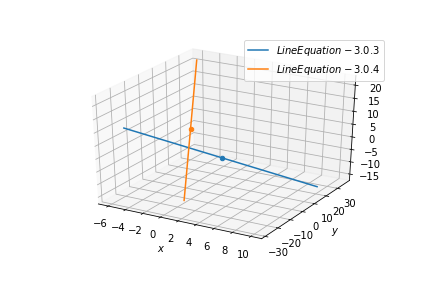
\includegraphics[width=\columnwidth]{./solutions/line_plane/74/codes/figs/Line_interest_1.png}
	\caption{Graph for equations \ref{eq:solutions/line_plane/74/codes7}}
	\label{fig:solutions/line_plane/74/codesline_equation_1}
\end{figure}


	\item 
	\begin{align}\label{eq:solutions/line_plane/74/codes12}
		\frac{x}{2} = \frac{y}{2} &= \frac{z}{1}, 
	\end{align}
	\begin{align}\label{eq:solutions/line_plane/74/codes13}
		\frac{x-5}{4} = \frac{y-2}{1} &= \frac{z-3}{8} 
	\end{align}



The above symmetric equations \ref{eq:solutions/line_plane/74/codes12}, \ref{eq:solutions/line_plane/74/codes13} can be represented in the vector form as 
\begin{align}\label{eq:solutions/line_plane/74/codes14}
	\quad \vec{r_1} &= \myvec{0\\0\\0} + \lambda_1\myvec{2\\2\\1}
	\\
	\quad \vec{r_2} &= \myvec{5\\2\\3} + \lambda_2\myvec{4\\1\\8}
\end{align}

As we have to find the angle between the vectors, we will only be taking the direction vectors into consideration. The direction vectors are $\vec{u}$ = $\myvec{2\\2\\1}$ and $\vec{v}$ = $\myvec{4\\1\\8}$. We can find the corresponding magnitude values

\begin{align}\label{eq:solutions/line_plane/74/codes16}
	\norm{\vec{u}} =\sqrt{2^{2}+2^{2}+1^{2}} =\sqrt{9}
\end{align}
\begin{align}\label{eq:solutions/line_plane/74/codes17}
	\norm{\vec{v}} =\sqrt{4^{2}+1^{2}+8^{2}} =\sqrt{81}
\end{align}

Using \ref{eq:solutions/line_plane/74/codes4}, \ref{eq:solutions/line_plane/74/codes16}, \ref{eq:solutions/line_plane/74/codes17} we get
\begin{align}
	\theta = \cos ^{-1}\frac{\myvec{2\\2\\1}^{T}\myvec{4\\1\\8}}{(\sqrt{9})(\sqrt{81})} 
	\\
	\theta = \cos ^{-1}\frac{18}{27.00}
	\\
	\theta = \cos ^{-1} (0.667)
	\\
	\theta = 48.189\degree
\end{align}

Therefore, the angle between the two lines is $48.189\degree$. See Fig. \ref{fig:solutions/line_plane/74/codesline_equation_2}


\begin{figure}
	\centering
	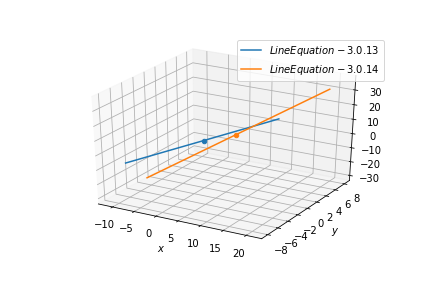
\includegraphics[width=\columnwidth]{./solutions/line_plane/74/codes/figs/Line_interest_2.png}
	\caption{Graph for equations \ref{eq:solutions/line_plane/74/codes14}}
	\label{fig:solutions/line_plane/74/codesline_equation_2}
\end{figure}
\end{enumerate}

    

%
\item For which value of $k$ will the following pair of linear equations have no solution?
\begin{align}
\begin{split}
\myvec{3 & 1 }\vec{x}&=1
\\
\myvec{2k-1 & k-1 }\vec{x}&=2k+1
\end{split}
\end{align}
\\
\solution
From theory, we understand that using dot product we can find the angle between the lines 
\begin{enumerate}
	\item 
	\begin{align}\label{eq:solutions/line_plane/74/codes:5}
		\frac{x-2}{2} = \frac{y-1}{5} &= \frac{z+3}{-3}, 
	\end{align}
	\begin{align}\label{eq:solutions/line_plane/74/codes:6}
		\frac{x+2}{-1} = \frac{y-4}{8} &= \frac{z-5}{4} 
	\end{align}


The above symmetric equations \ref{eq:solutions/line_plane/74/codes:5}, \ref{eq:solutions/line_plane/74/codes:6} can be represented in the vector form as 
\begin{align}\label{eq:solutions/line_plane/74/codes7}
	\quad \vec{r_1} &= \myvec{2\\1\\-3} + \lambda_1\myvec{2\\5\\-3}
	\\
	\quad \vec{r_2} &= \myvec{-2\\4\\5} + \lambda_2\myvec{-1\\8\\4}
\end{align}

As we have to find the angle between the vectors, we will only be taking the direction vectors into consideration. The direction vectors are $\vec{u}$ = $\myvec{2\\5\\-3}$ and $\vec{v}$ = $\myvec{-1\\8\\4}$. We can find the corresponding magnitude values

\begin{align}\label{eq:solutions/line_plane/74/codes9}
	\norm{\vec{u}} =\sqrt{2^{2}+5^{2}+(-3)^{2}} =\sqrt{38}
\end{align}
\begin{align}\label{eq:solutions/line_plane/74/codes10}
	\norm{\vec{v}} =\sqrt{(-1)^{2}+8^{2}+4^{2}} =\sqrt{81}
\end{align}

Using \ref{eq:solutions/line_plane/74/codes4}, \ref{eq:solutions/line_plane/74/codes9}, \ref{eq:solutions/line_plane/74/codes10} we get
\begin{align}
	\theta = \cos ^{-1}\frac{\myvec{2\\5\\-3}^{T}\myvec{-1\\8\\4}}{(\sqrt{38})(\sqrt{81})} 
	\\
	\theta = \cos ^{-1}\frac{26}{55.4797}
	\\
	\theta = \cos ^{-1} (0.4686)
	\\
	\theta = 62.053\degree
\end{align}

Therefore, the angle between the two lines is $62.053\degree$.See Fig. \ref{fig:solutions/line_plane/74/codesline_equation_1}

\begin{figure}
	\centering
	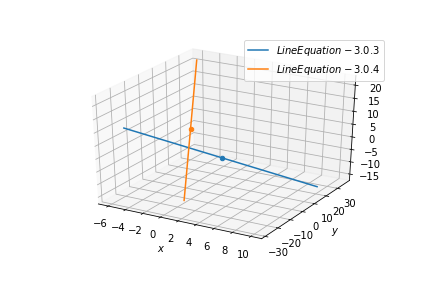
\includegraphics[width=\columnwidth]{./solutions/line_plane/74/codes/figs/Line_interest_1.png}
	\caption{Graph for equations \ref{eq:solutions/line_plane/74/codes7}}
	\label{fig:solutions/line_plane/74/codesline_equation_1}
\end{figure}


	\item 
	\begin{align}\label{eq:solutions/line_plane/74/codes12}
		\frac{x}{2} = \frac{y}{2} &= \frac{z}{1}, 
	\end{align}
	\begin{align}\label{eq:solutions/line_plane/74/codes13}
		\frac{x-5}{4} = \frac{y-2}{1} &= \frac{z-3}{8} 
	\end{align}



The above symmetric equations \ref{eq:solutions/line_plane/74/codes12}, \ref{eq:solutions/line_plane/74/codes13} can be represented in the vector form as 
\begin{align}\label{eq:solutions/line_plane/74/codes14}
	\quad \vec{r_1} &= \myvec{0\\0\\0} + \lambda_1\myvec{2\\2\\1}
	\\
	\quad \vec{r_2} &= \myvec{5\\2\\3} + \lambda_2\myvec{4\\1\\8}
\end{align}

As we have to find the angle between the vectors, we will only be taking the direction vectors into consideration. The direction vectors are $\vec{u}$ = $\myvec{2\\2\\1}$ and $\vec{v}$ = $\myvec{4\\1\\8}$. We can find the corresponding magnitude values

\begin{align}\label{eq:solutions/line_plane/74/codes16}
	\norm{\vec{u}} =\sqrt{2^{2}+2^{2}+1^{2}} =\sqrt{9}
\end{align}
\begin{align}\label{eq:solutions/line_plane/74/codes17}
	\norm{\vec{v}} =\sqrt{4^{2}+1^{2}+8^{2}} =\sqrt{81}
\end{align}

Using \ref{eq:solutions/line_plane/74/codes4}, \ref{eq:solutions/line_plane/74/codes16}, \ref{eq:solutions/line_plane/74/codes17} we get
\begin{align}
	\theta = \cos ^{-1}\frac{\myvec{2\\2\\1}^{T}\myvec{4\\1\\8}}{(\sqrt{9})(\sqrt{81})} 
	\\
	\theta = \cos ^{-1}\frac{18}{27.00}
	\\
	\theta = \cos ^{-1} (0.667)
	\\
	\theta = 48.189\degree
\end{align}

Therefore, the angle between the two lines is $48.189\degree$. See Fig. \ref{fig:solutions/line_plane/74/codesline_equation_2}


\begin{figure}
	\centering
	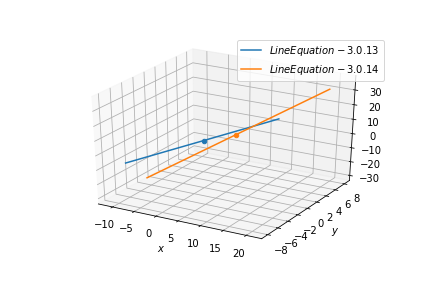
\includegraphics[width=\columnwidth]{./solutions/line_plane/74/codes/figs/Line_interest_2.png}
	\caption{Graph for equations \ref{eq:solutions/line_plane/74/codes14}}
	\label{fig:solutions/line_plane/74/codesline_equation_2}
\end{figure}
\end{enumerate}

    

\item Solve the following pair of linear equations
\begin{align}
\begin{split}
\myvec{8 & 5 }\vec{x}&=9
\\
\myvec{3 & 2 }\vec{x}&=4
\end{split}
\end{align}
\solution 
From theory, we understand that using dot product we can find the angle between the lines 
\begin{enumerate}
	\item 
	\begin{align}\label{eq:solutions/line_plane/74/codes:5}
		\frac{x-2}{2} = \frac{y-1}{5} &= \frac{z+3}{-3}, 
	\end{align}
	\begin{align}\label{eq:solutions/line_plane/74/codes:6}
		\frac{x+2}{-1} = \frac{y-4}{8} &= \frac{z-5}{4} 
	\end{align}


The above symmetric equations \ref{eq:solutions/line_plane/74/codes:5}, \ref{eq:solutions/line_plane/74/codes:6} can be represented in the vector form as 
\begin{align}\label{eq:solutions/line_plane/74/codes7}
	\quad \vec{r_1} &= \myvec{2\\1\\-3} + \lambda_1\myvec{2\\5\\-3}
	\\
	\quad \vec{r_2} &= \myvec{-2\\4\\5} + \lambda_2\myvec{-1\\8\\4}
\end{align}

As we have to find the angle between the vectors, we will only be taking the direction vectors into consideration. The direction vectors are $\vec{u}$ = $\myvec{2\\5\\-3}$ and $\vec{v}$ = $\myvec{-1\\8\\4}$. We can find the corresponding magnitude values

\begin{align}\label{eq:solutions/line_plane/74/codes9}
	\norm{\vec{u}} =\sqrt{2^{2}+5^{2}+(-3)^{2}} =\sqrt{38}
\end{align}
\begin{align}\label{eq:solutions/line_plane/74/codes10}
	\norm{\vec{v}} =\sqrt{(-1)^{2}+8^{2}+4^{2}} =\sqrt{81}
\end{align}

Using \ref{eq:solutions/line_plane/74/codes4}, \ref{eq:solutions/line_plane/74/codes9}, \ref{eq:solutions/line_plane/74/codes10} we get
\begin{align}
	\theta = \cos ^{-1}\frac{\myvec{2\\5\\-3}^{T}\myvec{-1\\8\\4}}{(\sqrt{38})(\sqrt{81})} 
	\\
	\theta = \cos ^{-1}\frac{26}{55.4797}
	\\
	\theta = \cos ^{-1} (0.4686)
	\\
	\theta = 62.053\degree
\end{align}

Therefore, the angle between the two lines is $62.053\degree$.See Fig. \ref{fig:solutions/line_plane/74/codesline_equation_1}

\begin{figure}
	\centering
	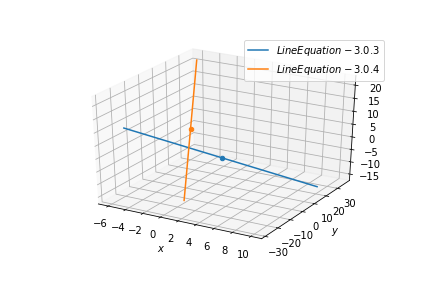
\includegraphics[width=\columnwidth]{./solutions/line_plane/74/codes/figs/Line_interest_1.png}
	\caption{Graph for equations \ref{eq:solutions/line_plane/74/codes7}}
	\label{fig:solutions/line_plane/74/codesline_equation_1}
\end{figure}


	\item 
	\begin{align}\label{eq:solutions/line_plane/74/codes12}
		\frac{x}{2} = \frac{y}{2} &= \frac{z}{1}, 
	\end{align}
	\begin{align}\label{eq:solutions/line_plane/74/codes13}
		\frac{x-5}{4} = \frac{y-2}{1} &= \frac{z-3}{8} 
	\end{align}



The above symmetric equations \ref{eq:solutions/line_plane/74/codes12}, \ref{eq:solutions/line_plane/74/codes13} can be represented in the vector form as 
\begin{align}\label{eq:solutions/line_plane/74/codes14}
	\quad \vec{r_1} &= \myvec{0\\0\\0} + \lambda_1\myvec{2\\2\\1}
	\\
	\quad \vec{r_2} &= \myvec{5\\2\\3} + \lambda_2\myvec{4\\1\\8}
\end{align}

As we have to find the angle between the vectors, we will only be taking the direction vectors into consideration. The direction vectors are $\vec{u}$ = $\myvec{2\\2\\1}$ and $\vec{v}$ = $\myvec{4\\1\\8}$. We can find the corresponding magnitude values

\begin{align}\label{eq:solutions/line_plane/74/codes16}
	\norm{\vec{u}} =\sqrt{2^{2}+2^{2}+1^{2}} =\sqrt{9}
\end{align}
\begin{align}\label{eq:solutions/line_plane/74/codes17}
	\norm{\vec{v}} =\sqrt{4^{2}+1^{2}+8^{2}} =\sqrt{81}
\end{align}

Using \ref{eq:solutions/line_plane/74/codes4}, \ref{eq:solutions/line_plane/74/codes16}, \ref{eq:solutions/line_plane/74/codes17} we get
\begin{align}
	\theta = \cos ^{-1}\frac{\myvec{2\\2\\1}^{T}\myvec{4\\1\\8}}{(\sqrt{9})(\sqrt{81})} 
	\\
	\theta = \cos ^{-1}\frac{18}{27.00}
	\\
	\theta = \cos ^{-1} (0.667)
	\\
	\theta = 48.189\degree
\end{align}

Therefore, the angle between the two lines is $48.189\degree$. See Fig. \ref{fig:solutions/line_plane/74/codesline_equation_2}


\begin{figure}
	\centering
	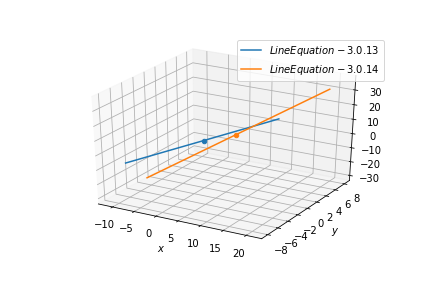
\includegraphics[width=\columnwidth]{./solutions/line_plane/74/codes/figs/Line_interest_2.png}
	\caption{Graph for equations \ref{eq:solutions/line_plane/74/codes14}}
	\label{fig:solutions/line_plane/74/codesline_equation_2}
\end{figure}
\end{enumerate}

    

%
\item Solve the following pair of linear equations
\begin{align}
\begin{split}
\myvec{158 & -378 }\vec{x}&=-74
\\
\myvec{-378 & 152 }\vec{x}&=-604
\end{split}
\end{align}
\solution 
From theory, we understand that using dot product we can find the angle between the lines 
\begin{enumerate}
	\item 
	\begin{align}\label{eq:solutions/line_plane/74/codes:5}
		\frac{x-2}{2} = \frac{y-1}{5} &= \frac{z+3}{-3}, 
	\end{align}
	\begin{align}\label{eq:solutions/line_plane/74/codes:6}
		\frac{x+2}{-1} = \frac{y-4}{8} &= \frac{z-5}{4} 
	\end{align}


The above symmetric equations \ref{eq:solutions/line_plane/74/codes:5}, \ref{eq:solutions/line_plane/74/codes:6} can be represented in the vector form as 
\begin{align}\label{eq:solutions/line_plane/74/codes7}
	\quad \vec{r_1} &= \myvec{2\\1\\-3} + \lambda_1\myvec{2\\5\\-3}
	\\
	\quad \vec{r_2} &= \myvec{-2\\4\\5} + \lambda_2\myvec{-1\\8\\4}
\end{align}

As we have to find the angle between the vectors, we will only be taking the direction vectors into consideration. The direction vectors are $\vec{u}$ = $\myvec{2\\5\\-3}$ and $\vec{v}$ = $\myvec{-1\\8\\4}$. We can find the corresponding magnitude values

\begin{align}\label{eq:solutions/line_plane/74/codes9}
	\norm{\vec{u}} =\sqrt{2^{2}+5^{2}+(-3)^{2}} =\sqrt{38}
\end{align}
\begin{align}\label{eq:solutions/line_plane/74/codes10}
	\norm{\vec{v}} =\sqrt{(-1)^{2}+8^{2}+4^{2}} =\sqrt{81}
\end{align}

Using \ref{eq:solutions/line_plane/74/codes4}, \ref{eq:solutions/line_plane/74/codes9}, \ref{eq:solutions/line_plane/74/codes10} we get
\begin{align}
	\theta = \cos ^{-1}\frac{\myvec{2\\5\\-3}^{T}\myvec{-1\\8\\4}}{(\sqrt{38})(\sqrt{81})} 
	\\
	\theta = \cos ^{-1}\frac{26}{55.4797}
	\\
	\theta = \cos ^{-1} (0.4686)
	\\
	\theta = 62.053\degree
\end{align}

Therefore, the angle between the two lines is $62.053\degree$.See Fig. \ref{fig:solutions/line_plane/74/codesline_equation_1}

\begin{figure}
	\centering
	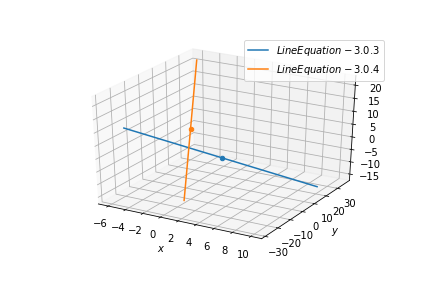
\includegraphics[width=\columnwidth]{./solutions/line_plane/74/codes/figs/Line_interest_1.png}
	\caption{Graph for equations \ref{eq:solutions/line_plane/74/codes7}}
	\label{fig:solutions/line_plane/74/codesline_equation_1}
\end{figure}


	\item 
	\begin{align}\label{eq:solutions/line_plane/74/codes12}
		\frac{x}{2} = \frac{y}{2} &= \frac{z}{1}, 
	\end{align}
	\begin{align}\label{eq:solutions/line_plane/74/codes13}
		\frac{x-5}{4} = \frac{y-2}{1} &= \frac{z-3}{8} 
	\end{align}



The above symmetric equations \ref{eq:solutions/line_plane/74/codes12}, \ref{eq:solutions/line_plane/74/codes13} can be represented in the vector form as 
\begin{align}\label{eq:solutions/line_plane/74/codes14}
	\quad \vec{r_1} &= \myvec{0\\0\\0} + \lambda_1\myvec{2\\2\\1}
	\\
	\quad \vec{r_2} &= \myvec{5\\2\\3} + \lambda_2\myvec{4\\1\\8}
\end{align}

As we have to find the angle between the vectors, we will only be taking the direction vectors into consideration. The direction vectors are $\vec{u}$ = $\myvec{2\\2\\1}$ and $\vec{v}$ = $\myvec{4\\1\\8}$. We can find the corresponding magnitude values

\begin{align}\label{eq:solutions/line_plane/74/codes16}
	\norm{\vec{u}} =\sqrt{2^{2}+2^{2}+1^{2}} =\sqrt{9}
\end{align}
\begin{align}\label{eq:solutions/line_plane/74/codes17}
	\norm{\vec{v}} =\sqrt{4^{2}+1^{2}+8^{2}} =\sqrt{81}
\end{align}

Using \ref{eq:solutions/line_plane/74/codes4}, \ref{eq:solutions/line_plane/74/codes16}, \ref{eq:solutions/line_plane/74/codes17} we get
\begin{align}
	\theta = \cos ^{-1}\frac{\myvec{2\\2\\1}^{T}\myvec{4\\1\\8}}{(\sqrt{9})(\sqrt{81})} 
	\\
	\theta = \cos ^{-1}\frac{18}{27.00}
	\\
	\theta = \cos ^{-1} (0.667)
	\\
	\theta = 48.189\degree
\end{align}

Therefore, the angle between the two lines is $48.189\degree$. See Fig. \ref{fig:solutions/line_plane/74/codesline_equation_2}


\begin{figure}
	\centering
	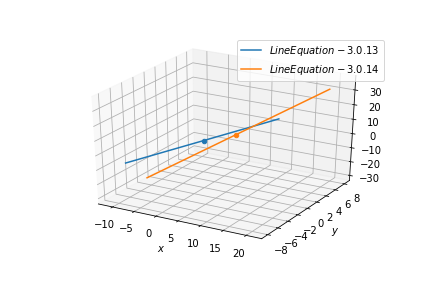
\includegraphics[width=\columnwidth]{./solutions/line_plane/74/codes/figs/Line_interest_2.png}
	\caption{Graph for equations \ref{eq:solutions/line_plane/74/codes14}}
	\label{fig:solutions/line_plane/74/codesline_equation_2}
\end{figure}
\end{enumerate}

    


\item  Find the slope of a line, which passes through the origin, and the mid-point of the line segment joining the points $\vec{P} = \myvec{0\\ – 4}$ and $\vec{B} = \myvec{8\\ 0}$.
\solution 
From theory, we understand that using dot product we can find the angle between the lines 
\begin{enumerate}
	\item 
	\begin{align}\label{eq:solutions/line_plane/74/codes:5}
		\frac{x-2}{2} = \frac{y-1}{5} &= \frac{z+3}{-3}, 
	\end{align}
	\begin{align}\label{eq:solutions/line_plane/74/codes:6}
		\frac{x+2}{-1} = \frac{y-4}{8} &= \frac{z-5}{4} 
	\end{align}


The above symmetric equations \ref{eq:solutions/line_plane/74/codes:5}, \ref{eq:solutions/line_plane/74/codes:6} can be represented in the vector form as 
\begin{align}\label{eq:solutions/line_plane/74/codes7}
	\quad \vec{r_1} &= \myvec{2\\1\\-3} + \lambda_1\myvec{2\\5\\-3}
	\\
	\quad \vec{r_2} &= \myvec{-2\\4\\5} + \lambda_2\myvec{-1\\8\\4}
\end{align}

As we have to find the angle between the vectors, we will only be taking the direction vectors into consideration. The direction vectors are $\vec{u}$ = $\myvec{2\\5\\-3}$ and $\vec{v}$ = $\myvec{-1\\8\\4}$. We can find the corresponding magnitude values

\begin{align}\label{eq:solutions/line_plane/74/codes9}
	\norm{\vec{u}} =\sqrt{2^{2}+5^{2}+(-3)^{2}} =\sqrt{38}
\end{align}
\begin{align}\label{eq:solutions/line_plane/74/codes10}
	\norm{\vec{v}} =\sqrt{(-1)^{2}+8^{2}+4^{2}} =\sqrt{81}
\end{align}

Using \ref{eq:solutions/line_plane/74/codes4}, \ref{eq:solutions/line_plane/74/codes9}, \ref{eq:solutions/line_plane/74/codes10} we get
\begin{align}
	\theta = \cos ^{-1}\frac{\myvec{2\\5\\-3}^{T}\myvec{-1\\8\\4}}{(\sqrt{38})(\sqrt{81})} 
	\\
	\theta = \cos ^{-1}\frac{26}{55.4797}
	\\
	\theta = \cos ^{-1} (0.4686)
	\\
	\theta = 62.053\degree
\end{align}

Therefore, the angle between the two lines is $62.053\degree$.See Fig. \ref{fig:solutions/line_plane/74/codesline_equation_1}

\begin{figure}
	\centering
	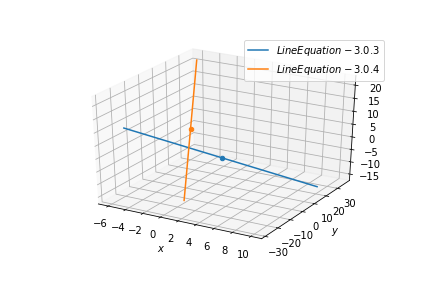
\includegraphics[width=\columnwidth]{./solutions/line_plane/74/codes/figs/Line_interest_1.png}
	\caption{Graph for equations \ref{eq:solutions/line_plane/74/codes7}}
	\label{fig:solutions/line_plane/74/codesline_equation_1}
\end{figure}


	\item 
	\begin{align}\label{eq:solutions/line_plane/74/codes12}
		\frac{x}{2} = \frac{y}{2} &= \frac{z}{1}, 
	\end{align}
	\begin{align}\label{eq:solutions/line_plane/74/codes13}
		\frac{x-5}{4} = \frac{y-2}{1} &= \frac{z-3}{8} 
	\end{align}



The above symmetric equations \ref{eq:solutions/line_plane/74/codes12}, \ref{eq:solutions/line_plane/74/codes13} can be represented in the vector form as 
\begin{align}\label{eq:solutions/line_plane/74/codes14}
	\quad \vec{r_1} &= \myvec{0\\0\\0} + \lambda_1\myvec{2\\2\\1}
	\\
	\quad \vec{r_2} &= \myvec{5\\2\\3} + \lambda_2\myvec{4\\1\\8}
\end{align}

As we have to find the angle between the vectors, we will only be taking the direction vectors into consideration. The direction vectors are $\vec{u}$ = $\myvec{2\\2\\1}$ and $\vec{v}$ = $\myvec{4\\1\\8}$. We can find the corresponding magnitude values

\begin{align}\label{eq:solutions/line_plane/74/codes16}
	\norm{\vec{u}} =\sqrt{2^{2}+2^{2}+1^{2}} =\sqrt{9}
\end{align}
\begin{align}\label{eq:solutions/line_plane/74/codes17}
	\norm{\vec{v}} =\sqrt{4^{2}+1^{2}+8^{2}} =\sqrt{81}
\end{align}

Using \ref{eq:solutions/line_plane/74/codes4}, \ref{eq:solutions/line_plane/74/codes16}, \ref{eq:solutions/line_plane/74/codes17} we get
\begin{align}
	\theta = \cos ^{-1}\frac{\myvec{2\\2\\1}^{T}\myvec{4\\1\\8}}{(\sqrt{9})(\sqrt{81})} 
	\\
	\theta = \cos ^{-1}\frac{18}{27.00}
	\\
	\theta = \cos ^{-1} (0.667)
	\\
	\theta = 48.189\degree
\end{align}

Therefore, the angle between the two lines is $48.189\degree$. See Fig. \ref{fig:solutions/line_plane/74/codesline_equation_2}


\begin{figure}
	\centering
	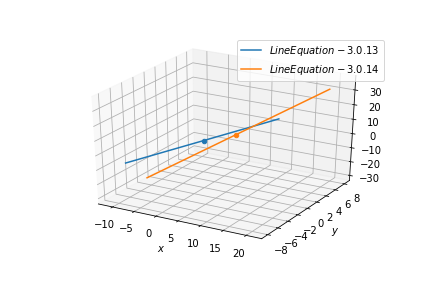
\includegraphics[width=\columnwidth]{./solutions/line_plane/74/codes/figs/Line_interest_2.png}
	\caption{Graph for equations \ref{eq:solutions/line_plane/74/codes14}}
	\label{fig:solutions/line_plane/74/codesline_equation_2}
\end{figure}
\end{enumerate}

    

\item The slope of a line is double of the slope of another line. If the tangent of the angle
between them is $\frac{1}{3}$, find the slopes of the lines.
\solution 
From theory, we understand that using dot product we can find the angle between the lines 
\begin{enumerate}
	\item 
	\begin{align}\label{eq:solutions/line_plane/74/codes:5}
		\frac{x-2}{2} = \frac{y-1}{5} &= \frac{z+3}{-3}, 
	\end{align}
	\begin{align}\label{eq:solutions/line_plane/74/codes:6}
		\frac{x+2}{-1} = \frac{y-4}{8} &= \frac{z-5}{4} 
	\end{align}


The above symmetric equations \ref{eq:solutions/line_plane/74/codes:5}, \ref{eq:solutions/line_plane/74/codes:6} can be represented in the vector form as 
\begin{align}\label{eq:solutions/line_plane/74/codes7}
	\quad \vec{r_1} &= \myvec{2\\1\\-3} + \lambda_1\myvec{2\\5\\-3}
	\\
	\quad \vec{r_2} &= \myvec{-2\\4\\5} + \lambda_2\myvec{-1\\8\\4}
\end{align}

As we have to find the angle between the vectors, we will only be taking the direction vectors into consideration. The direction vectors are $\vec{u}$ = $\myvec{2\\5\\-3}$ and $\vec{v}$ = $\myvec{-1\\8\\4}$. We can find the corresponding magnitude values

\begin{align}\label{eq:solutions/line_plane/74/codes9}
	\norm{\vec{u}} =\sqrt{2^{2}+5^{2}+(-3)^{2}} =\sqrt{38}
\end{align}
\begin{align}\label{eq:solutions/line_plane/74/codes10}
	\norm{\vec{v}} =\sqrt{(-1)^{2}+8^{2}+4^{2}} =\sqrt{81}
\end{align}

Using \ref{eq:solutions/line_plane/74/codes4}, \ref{eq:solutions/line_plane/74/codes9}, \ref{eq:solutions/line_plane/74/codes10} we get
\begin{align}
	\theta = \cos ^{-1}\frac{\myvec{2\\5\\-3}^{T}\myvec{-1\\8\\4}}{(\sqrt{38})(\sqrt{81})} 
	\\
	\theta = \cos ^{-1}\frac{26}{55.4797}
	\\
	\theta = \cos ^{-1} (0.4686)
	\\
	\theta = 62.053\degree
\end{align}

Therefore, the angle between the two lines is $62.053\degree$.See Fig. \ref{fig:solutions/line_plane/74/codesline_equation_1}

\begin{figure}
	\centering
	\includegraphics[width=\columnwidth]{./solutions/line_plane/74/codes/figs/Line_interest_1.png}
	\caption{Graph for equations \ref{eq:solutions/line_plane/74/codes7}}
	\label{fig:solutions/line_plane/74/codesline_equation_1}
\end{figure}


	\item 
	\begin{align}\label{eq:solutions/line_plane/74/codes12}
		\frac{x}{2} = \frac{y}{2} &= \frac{z}{1}, 
	\end{align}
	\begin{align}\label{eq:solutions/line_plane/74/codes13}
		\frac{x-5}{4} = \frac{y-2}{1} &= \frac{z-3}{8} 
	\end{align}



The above symmetric equations \ref{eq:solutions/line_plane/74/codes12}, \ref{eq:solutions/line_plane/74/codes13} can be represented in the vector form as 
\begin{align}\label{eq:solutions/line_plane/74/codes14}
	\quad \vec{r_1} &= \myvec{0\\0\\0} + \lambda_1\myvec{2\\2\\1}
	\\
	\quad \vec{r_2} &= \myvec{5\\2\\3} + \lambda_2\myvec{4\\1\\8}
\end{align}

As we have to find the angle between the vectors, we will only be taking the direction vectors into consideration. The direction vectors are $\vec{u}$ = $\myvec{2\\2\\1}$ and $\vec{v}$ = $\myvec{4\\1\\8}$. We can find the corresponding magnitude values

\begin{align}\label{eq:solutions/line_plane/74/codes16}
	\norm{\vec{u}} =\sqrt{2^{2}+2^{2}+1^{2}} =\sqrt{9}
\end{align}
\begin{align}\label{eq:solutions/line_plane/74/codes17}
	\norm{\vec{v}} =\sqrt{4^{2}+1^{2}+8^{2}} =\sqrt{81}
\end{align}

Using \ref{eq:solutions/line_plane/74/codes4}, \ref{eq:solutions/line_plane/74/codes16}, \ref{eq:solutions/line_plane/74/codes17} we get
\begin{align}
	\theta = \cos ^{-1}\frac{\myvec{2\\2\\1}^{T}\myvec{4\\1\\8}}{(\sqrt{9})(\sqrt{81})} 
	\\
	\theta = \cos ^{-1}\frac{18}{27.00}
	\\
	\theta = \cos ^{-1} (0.667)
	\\
	\theta = 48.189\degree
\end{align}

Therefore, the angle between the two lines is $48.189\degree$. See Fig. \ref{fig:solutions/line_plane/74/codesline_equation_2}


\begin{figure}
	\centering
	\includegraphics[width=\columnwidth]{./solutions/line_plane/74/codes/figs/Line_interest_2.png}
	\caption{Graph for equations \ref{eq:solutions/line_plane/74/codes14}}
	\label{fig:solutions/line_plane/74/codesline_equation_2}
\end{figure}
\end{enumerate}

    

\item Find the intercepts of the following  lines on the axes.
\begin{enumerate}
\item $\myvec{3 & 2}\vec{x} = 12$.
\item $\myvec{4 & -3}\vec{x} = 6$.
\item $\myvec{3 & 2}\vec{x} = 0$.
\end{enumerate}
\solution
From theory, we understand that using dot product we can find the angle between the lines 
\begin{enumerate}
	\item 
	\begin{align}\label{eq:solutions/line_plane/74/codes:5}
		\frac{x-2}{2} = \frac{y-1}{5} &= \frac{z+3}{-3}, 
	\end{align}
	\begin{align}\label{eq:solutions/line_plane/74/codes:6}
		\frac{x+2}{-1} = \frac{y-4}{8} &= \frac{z-5}{4} 
	\end{align}


The above symmetric equations \ref{eq:solutions/line_plane/74/codes:5}, \ref{eq:solutions/line_plane/74/codes:6} can be represented in the vector form as 
\begin{align}\label{eq:solutions/line_plane/74/codes7}
	\quad \vec{r_1} &= \myvec{2\\1\\-3} + \lambda_1\myvec{2\\5\\-3}
	\\
	\quad \vec{r_2} &= \myvec{-2\\4\\5} + \lambda_2\myvec{-1\\8\\4}
\end{align}

As we have to find the angle between the vectors, we will only be taking the direction vectors into consideration. The direction vectors are $\vec{u}$ = $\myvec{2\\5\\-3}$ and $\vec{v}$ = $\myvec{-1\\8\\4}$. We can find the corresponding magnitude values

\begin{align}\label{eq:solutions/line_plane/74/codes9}
	\norm{\vec{u}} =\sqrt{2^{2}+5^{2}+(-3)^{2}} =\sqrt{38}
\end{align}
\begin{align}\label{eq:solutions/line_plane/74/codes10}
	\norm{\vec{v}} =\sqrt{(-1)^{2}+8^{2}+4^{2}} =\sqrt{81}
\end{align}

Using \ref{eq:solutions/line_plane/74/codes4}, \ref{eq:solutions/line_plane/74/codes9}, \ref{eq:solutions/line_plane/74/codes10} we get
\begin{align}
	\theta = \cos ^{-1}\frac{\myvec{2\\5\\-3}^{T}\myvec{-1\\8\\4}}{(\sqrt{38})(\sqrt{81})} 
	\\
	\theta = \cos ^{-1}\frac{26}{55.4797}
	\\
	\theta = \cos ^{-1} (0.4686)
	\\
	\theta = 62.053\degree
\end{align}

Therefore, the angle between the two lines is $62.053\degree$.See Fig. \ref{fig:solutions/line_plane/74/codesline_equation_1}

\begin{figure}
	\centering
	\includegraphics[width=\columnwidth]{./solutions/line_plane/74/codes/figs/Line_interest_1.png}
	\caption{Graph for equations \ref{eq:solutions/line_plane/74/codes7}}
	\label{fig:solutions/line_plane/74/codesline_equation_1}
\end{figure}


	\item 
	\begin{align}\label{eq:solutions/line_plane/74/codes12}
		\frac{x}{2} = \frac{y}{2} &= \frac{z}{1}, 
	\end{align}
	\begin{align}\label{eq:solutions/line_plane/74/codes13}
		\frac{x-5}{4} = \frac{y-2}{1} &= \frac{z-3}{8} 
	\end{align}



The above symmetric equations \ref{eq:solutions/line_plane/74/codes12}, \ref{eq:solutions/line_plane/74/codes13} can be represented in the vector form as 
\begin{align}\label{eq:solutions/line_plane/74/codes14}
	\quad \vec{r_1} &= \myvec{0\\0\\0} + \lambda_1\myvec{2\\2\\1}
	\\
	\quad \vec{r_2} &= \myvec{5\\2\\3} + \lambda_2\myvec{4\\1\\8}
\end{align}

As we have to find the angle between the vectors, we will only be taking the direction vectors into consideration. The direction vectors are $\vec{u}$ = $\myvec{2\\2\\1}$ and $\vec{v}$ = $\myvec{4\\1\\8}$. We can find the corresponding magnitude values

\begin{align}\label{eq:solutions/line_plane/74/codes16}
	\norm{\vec{u}} =\sqrt{2^{2}+2^{2}+1^{2}} =\sqrt{9}
\end{align}
\begin{align}\label{eq:solutions/line_plane/74/codes17}
	\norm{\vec{v}} =\sqrt{4^{2}+1^{2}+8^{2}} =\sqrt{81}
\end{align}

Using \ref{eq:solutions/line_plane/74/codes4}, \ref{eq:solutions/line_plane/74/codes16}, \ref{eq:solutions/line_plane/74/codes17} we get
\begin{align}
	\theta = \cos ^{-1}\frac{\myvec{2\\2\\1}^{T}\myvec{4\\1\\8}}{(\sqrt{9})(\sqrt{81})} 
	\\
	\theta = \cos ^{-1}\frac{18}{27.00}
	\\
	\theta = \cos ^{-1} (0.667)
	\\
	\theta = 48.189\degree
\end{align}

Therefore, the angle between the two lines is $48.189\degree$. See Fig. \ref{fig:solutions/line_plane/74/codesline_equation_2}


\begin{figure}
	\centering
	\includegraphics[width=\columnwidth]{./solutions/line_plane/74/codes/figs/Line_interest_2.png}
	\caption{Graph for equations \ref{eq:solutions/line_plane/74/codes14}}
	\label{fig:solutions/line_plane/74/codesline_equation_2}
\end{figure}
\end{enumerate}

    

\item Find the distance of the point \myvec{1\\-1} from the line $\myvec{12 & -5}\vec{x} = -82$.
\\
\solution
From theory, we understand that using dot product we can find the angle between the lines 
\begin{enumerate}
	\item 
	\begin{align}\label{eq:solutions/line_plane/74/codes:5}
		\frac{x-2}{2} = \frac{y-1}{5} &= \frac{z+3}{-3}, 
	\end{align}
	\begin{align}\label{eq:solutions/line_plane/74/codes:6}
		\frac{x+2}{-1} = \frac{y-4}{8} &= \frac{z-5}{4} 
	\end{align}


The above symmetric equations \ref{eq:solutions/line_plane/74/codes:5}, \ref{eq:solutions/line_plane/74/codes:6} can be represented in the vector form as 
\begin{align}\label{eq:solutions/line_plane/74/codes7}
	\quad \vec{r_1} &= \myvec{2\\1\\-3} + \lambda_1\myvec{2\\5\\-3}
	\\
	\quad \vec{r_2} &= \myvec{-2\\4\\5} + \lambda_2\myvec{-1\\8\\4}
\end{align}

As we have to find the angle between the vectors, we will only be taking the direction vectors into consideration. The direction vectors are $\vec{u}$ = $\myvec{2\\5\\-3}$ and $\vec{v}$ = $\myvec{-1\\8\\4}$. We can find the corresponding magnitude values

\begin{align}\label{eq:solutions/line_plane/74/codes9}
	\norm{\vec{u}} =\sqrt{2^{2}+5^{2}+(-3)^{2}} =\sqrt{38}
\end{align}
\begin{align}\label{eq:solutions/line_plane/74/codes10}
	\norm{\vec{v}} =\sqrt{(-1)^{2}+8^{2}+4^{2}} =\sqrt{81}
\end{align}

Using \ref{eq:solutions/line_plane/74/codes4}, \ref{eq:solutions/line_plane/74/codes9}, \ref{eq:solutions/line_plane/74/codes10} we get
\begin{align}
	\theta = \cos ^{-1}\frac{\myvec{2\\5\\-3}^{T}\myvec{-1\\8\\4}}{(\sqrt{38})(\sqrt{81})} 
	\\
	\theta = \cos ^{-1}\frac{26}{55.4797}
	\\
	\theta = \cos ^{-1} (0.4686)
	\\
	\theta = 62.053\degree
\end{align}

Therefore, the angle between the two lines is $62.053\degree$.See Fig. \ref{fig:solutions/line_plane/74/codesline_equation_1}

\begin{figure}
	\centering
	\includegraphics[width=\columnwidth]{./solutions/line_plane/74/codes/figs/Line_interest_1.png}
	\caption{Graph for equations \ref{eq:solutions/line_plane/74/codes7}}
	\label{fig:solutions/line_plane/74/codesline_equation_1}
\end{figure}


	\item 
	\begin{align}\label{eq:solutions/line_plane/74/codes12}
		\frac{x}{2} = \frac{y}{2} &= \frac{z}{1}, 
	\end{align}
	\begin{align}\label{eq:solutions/line_plane/74/codes13}
		\frac{x-5}{4} = \frac{y-2}{1} &= \frac{z-3}{8} 
	\end{align}



The above symmetric equations \ref{eq:solutions/line_plane/74/codes12}, \ref{eq:solutions/line_plane/74/codes13} can be represented in the vector form as 
\begin{align}\label{eq:solutions/line_plane/74/codes14}
	\quad \vec{r_1} &= \myvec{0\\0\\0} + \lambda_1\myvec{2\\2\\1}
	\\
	\quad \vec{r_2} &= \myvec{5\\2\\3} + \lambda_2\myvec{4\\1\\8}
\end{align}

As we have to find the angle between the vectors, we will only be taking the direction vectors into consideration. The direction vectors are $\vec{u}$ = $\myvec{2\\2\\1}$ and $\vec{v}$ = $\myvec{4\\1\\8}$. We can find the corresponding magnitude values

\begin{align}\label{eq:solutions/line_plane/74/codes16}
	\norm{\vec{u}} =\sqrt{2^{2}+2^{2}+1^{2}} =\sqrt{9}
\end{align}
\begin{align}\label{eq:solutions/line_plane/74/codes17}
	\norm{\vec{v}} =\sqrt{4^{2}+1^{2}+8^{2}} =\sqrt{81}
\end{align}

Using \ref{eq:solutions/line_plane/74/codes4}, \ref{eq:solutions/line_plane/74/codes16}, \ref{eq:solutions/line_plane/74/codes17} we get
\begin{align}
	\theta = \cos ^{-1}\frac{\myvec{2\\2\\1}^{T}\myvec{4\\1\\8}}{(\sqrt{9})(\sqrt{81})} 
	\\
	\theta = \cos ^{-1}\frac{18}{27.00}
	\\
	\theta = \cos ^{-1} (0.667)
	\\
	\theta = 48.189\degree
\end{align}

Therefore, the angle between the two lines is $48.189\degree$. See Fig. \ref{fig:solutions/line_plane/74/codesline_equation_2}


\begin{figure}
	\centering
	\includegraphics[width=\columnwidth]{./solutions/line_plane/74/codes/figs/Line_interest_2.png}
	\caption{Graph for equations \ref{eq:solutions/line_plane/74/codes14}}
	\label{fig:solutions/line_plane/74/codesline_equation_2}
\end{figure}
\end{enumerate}

    

\item Find the points on the x-axis, whose distances from the line 
\begin{align}
\myvec{4 & 3} \vec{x} = 12
\end{align}
are 4 units.
%
\\
\solution
From theory, we understand that using dot product we can find the angle between the lines 
\begin{enumerate}
	\item 
	\begin{align}\label{eq:solutions/line_plane/74/codes:5}
		\frac{x-2}{2} = \frac{y-1}{5} &= \frac{z+3}{-3}, 
	\end{align}
	\begin{align}\label{eq:solutions/line_plane/74/codes:6}
		\frac{x+2}{-1} = \frac{y-4}{8} &= \frac{z-5}{4} 
	\end{align}


The above symmetric equations \ref{eq:solutions/line_plane/74/codes:5}, \ref{eq:solutions/line_plane/74/codes:6} can be represented in the vector form as 
\begin{align}\label{eq:solutions/line_plane/74/codes7}
	\quad \vec{r_1} &= \myvec{2\\1\\-3} + \lambda_1\myvec{2\\5\\-3}
	\\
	\quad \vec{r_2} &= \myvec{-2\\4\\5} + \lambda_2\myvec{-1\\8\\4}
\end{align}

As we have to find the angle between the vectors, we will only be taking the direction vectors into consideration. The direction vectors are $\vec{u}$ = $\myvec{2\\5\\-3}$ and $\vec{v}$ = $\myvec{-1\\8\\4}$. We can find the corresponding magnitude values

\begin{align}\label{eq:solutions/line_plane/74/codes9}
	\norm{\vec{u}} =\sqrt{2^{2}+5^{2}+(-3)^{2}} =\sqrt{38}
\end{align}
\begin{align}\label{eq:solutions/line_plane/74/codes10}
	\norm{\vec{v}} =\sqrt{(-1)^{2}+8^{2}+4^{2}} =\sqrt{81}
\end{align}

Using \ref{eq:solutions/line_plane/74/codes4}, \ref{eq:solutions/line_plane/74/codes9}, \ref{eq:solutions/line_plane/74/codes10} we get
\begin{align}
	\theta = \cos ^{-1}\frac{\myvec{2\\5\\-3}^{T}\myvec{-1\\8\\4}}{(\sqrt{38})(\sqrt{81})} 
	\\
	\theta = \cos ^{-1}\frac{26}{55.4797}
	\\
	\theta = \cos ^{-1} (0.4686)
	\\
	\theta = 62.053\degree
\end{align}

Therefore, the angle between the two lines is $62.053\degree$.See Fig. \ref{fig:solutions/line_plane/74/codesline_equation_1}

\begin{figure}
	\centering
	\includegraphics[width=\columnwidth]{./solutions/line_plane/74/codes/figs/Line_interest_1.png}
	\caption{Graph for equations \ref{eq:solutions/line_plane/74/codes7}}
	\label{fig:solutions/line_plane/74/codesline_equation_1}
\end{figure}


	\item 
	\begin{align}\label{eq:solutions/line_plane/74/codes12}
		\frac{x}{2} = \frac{y}{2} &= \frac{z}{1}, 
	\end{align}
	\begin{align}\label{eq:solutions/line_plane/74/codes13}
		\frac{x-5}{4} = \frac{y-2}{1} &= \frac{z-3}{8} 
	\end{align}



The above symmetric equations \ref{eq:solutions/line_plane/74/codes12}, \ref{eq:solutions/line_plane/74/codes13} can be represented in the vector form as 
\begin{align}\label{eq:solutions/line_plane/74/codes14}
	\quad \vec{r_1} &= \myvec{0\\0\\0} + \lambda_1\myvec{2\\2\\1}
	\\
	\quad \vec{r_2} &= \myvec{5\\2\\3} + \lambda_2\myvec{4\\1\\8}
\end{align}

As we have to find the angle between the vectors, we will only be taking the direction vectors into consideration. The direction vectors are $\vec{u}$ = $\myvec{2\\2\\1}$ and $\vec{v}$ = $\myvec{4\\1\\8}$. We can find the corresponding magnitude values

\begin{align}\label{eq:solutions/line_plane/74/codes16}
	\norm{\vec{u}} =\sqrt{2^{2}+2^{2}+1^{2}} =\sqrt{9}
\end{align}
\begin{align}\label{eq:solutions/line_plane/74/codes17}
	\norm{\vec{v}} =\sqrt{4^{2}+1^{2}+8^{2}} =\sqrt{81}
\end{align}

Using \ref{eq:solutions/line_plane/74/codes4}, \ref{eq:solutions/line_plane/74/codes16}, \ref{eq:solutions/line_plane/74/codes17} we get
\begin{align}
	\theta = \cos ^{-1}\frac{\myvec{2\\2\\1}^{T}\myvec{4\\1\\8}}{(\sqrt{9})(\sqrt{81})} 
	\\
	\theta = \cos ^{-1}\frac{18}{27.00}
	\\
	\theta = \cos ^{-1} (0.667)
	\\
	\theta = 48.189\degree
\end{align}

Therefore, the angle between the two lines is $48.189\degree$. See Fig. \ref{fig:solutions/line_plane/74/codesline_equation_2}


\begin{figure}
	\centering
	\includegraphics[width=\columnwidth]{./solutions/line_plane/74/codes/figs/Line_interest_2.png}
	\caption{Graph for equations \ref{eq:solutions/line_plane/74/codes14}}
	\label{fig:solutions/line_plane/74/codesline_equation_2}
\end{figure}
\end{enumerate}

    

\item Find the equation of a line perpendicular to the line 
\begin{align}
\myvec{1 & -7}\vec{x} = -5
\end{align}
and having x intercept 3.
\\
\solution
From theory, we understand that using dot product we can find the angle between the lines 
\begin{enumerate}
	\item 
	\begin{align}\label{eq:solutions/line_plane/74/codes:5}
		\frac{x-2}{2} = \frac{y-1}{5} &= \frac{z+3}{-3}, 
	\end{align}
	\begin{align}\label{eq:solutions/line_plane/74/codes:6}
		\frac{x+2}{-1} = \frac{y-4}{8} &= \frac{z-5}{4} 
	\end{align}


The above symmetric equations \ref{eq:solutions/line_plane/74/codes:5}, \ref{eq:solutions/line_plane/74/codes:6} can be represented in the vector form as 
\begin{align}\label{eq:solutions/line_plane/74/codes7}
	\quad \vec{r_1} &= \myvec{2\\1\\-3} + \lambda_1\myvec{2\\5\\-3}
	\\
	\quad \vec{r_2} &= \myvec{-2\\4\\5} + \lambda_2\myvec{-1\\8\\4}
\end{align}

As we have to find the angle between the vectors, we will only be taking the direction vectors into consideration. The direction vectors are $\vec{u}$ = $\myvec{2\\5\\-3}$ and $\vec{v}$ = $\myvec{-1\\8\\4}$. We can find the corresponding magnitude values

\begin{align}\label{eq:solutions/line_plane/74/codes9}
	\norm{\vec{u}} =\sqrt{2^{2}+5^{2}+(-3)^{2}} =\sqrt{38}
\end{align}
\begin{align}\label{eq:solutions/line_plane/74/codes10}
	\norm{\vec{v}} =\sqrt{(-1)^{2}+8^{2}+4^{2}} =\sqrt{81}
\end{align}

Using \ref{eq:solutions/line_plane/74/codes4}, \ref{eq:solutions/line_plane/74/codes9}, \ref{eq:solutions/line_plane/74/codes10} we get
\begin{align}
	\theta = \cos ^{-1}\frac{\myvec{2\\5\\-3}^{T}\myvec{-1\\8\\4}}{(\sqrt{38})(\sqrt{81})} 
	\\
	\theta = \cos ^{-1}\frac{26}{55.4797}
	\\
	\theta = \cos ^{-1} (0.4686)
	\\
	\theta = 62.053\degree
\end{align}

Therefore, the angle between the two lines is $62.053\degree$.See Fig. \ref{fig:solutions/line_plane/74/codesline_equation_1}

\begin{figure}
	\centering
	\includegraphics[width=\columnwidth]{./solutions/line_plane/74/codes/figs/Line_interest_1.png}
	\caption{Graph for equations \ref{eq:solutions/line_plane/74/codes7}}
	\label{fig:solutions/line_plane/74/codesline_equation_1}
\end{figure}


	\item 
	\begin{align}\label{eq:solutions/line_plane/74/codes12}
		\frac{x}{2} = \frac{y}{2} &= \frac{z}{1}, 
	\end{align}
	\begin{align}\label{eq:solutions/line_plane/74/codes13}
		\frac{x-5}{4} = \frac{y-2}{1} &= \frac{z-3}{8} 
	\end{align}



The above symmetric equations \ref{eq:solutions/line_plane/74/codes12}, \ref{eq:solutions/line_plane/74/codes13} can be represented in the vector form as 
\begin{align}\label{eq:solutions/line_plane/74/codes14}
	\quad \vec{r_1} &= \myvec{0\\0\\0} + \lambda_1\myvec{2\\2\\1}
	\\
	\quad \vec{r_2} &= \myvec{5\\2\\3} + \lambda_2\myvec{4\\1\\8}
\end{align}

As we have to find the angle between the vectors, we will only be taking the direction vectors into consideration. The direction vectors are $\vec{u}$ = $\myvec{2\\2\\1}$ and $\vec{v}$ = $\myvec{4\\1\\8}$. We can find the corresponding magnitude values

\begin{align}\label{eq:solutions/line_plane/74/codes16}
	\norm{\vec{u}} =\sqrt{2^{2}+2^{2}+1^{2}} =\sqrt{9}
\end{align}
\begin{align}\label{eq:solutions/line_plane/74/codes17}
	\norm{\vec{v}} =\sqrt{4^{2}+1^{2}+8^{2}} =\sqrt{81}
\end{align}

Using \ref{eq:solutions/line_plane/74/codes4}, \ref{eq:solutions/line_plane/74/codes16}, \ref{eq:solutions/line_plane/74/codes17} we get
\begin{align}
	\theta = \cos ^{-1}\frac{\myvec{2\\2\\1}^{T}\myvec{4\\1\\8}}{(\sqrt{9})(\sqrt{81})} 
	\\
	\theta = \cos ^{-1}\frac{18}{27.00}
	\\
	\theta = \cos ^{-1} (0.667)
	\\
	\theta = 48.189\degree
\end{align}

Therefore, the angle between the two lines is $48.189\degree$. See Fig. \ref{fig:solutions/line_plane/74/codesline_equation_2}


\begin{figure}
	\centering
	\includegraphics[width=\columnwidth]{./solutions/line_plane/74/codes/figs/Line_interest_2.png}
	\caption{Graph for equations \ref{eq:solutions/line_plane/74/codes14}}
	\label{fig:solutions/line_plane/74/codesline_equation_2}
\end{figure}
\end{enumerate}

    

\item Find angles between the lines
\begin{align}
\myvec{\sqrt{3} & 1}\vec{x} &= 1
\\
\myvec{1 & \sqrt{3}}\vec{x} &= 1
\end{align}
\\
\solution
From theory, we understand that using dot product we can find the angle between the lines 
\begin{enumerate}
	\item 
	\begin{align}\label{eq:solutions/line_plane/74/codes:5}
		\frac{x-2}{2} = \frac{y-1}{5} &= \frac{z+3}{-3}, 
	\end{align}
	\begin{align}\label{eq:solutions/line_plane/74/codes:6}
		\frac{x+2}{-1} = \frac{y-4}{8} &= \frac{z-5}{4} 
	\end{align}


The above symmetric equations \ref{eq:solutions/line_plane/74/codes:5}, \ref{eq:solutions/line_plane/74/codes:6} can be represented in the vector form as 
\begin{align}\label{eq:solutions/line_plane/74/codes7}
	\quad \vec{r_1} &= \myvec{2\\1\\-3} + \lambda_1\myvec{2\\5\\-3}
	\\
	\quad \vec{r_2} &= \myvec{-2\\4\\5} + \lambda_2\myvec{-1\\8\\4}
\end{align}

As we have to find the angle between the vectors, we will only be taking the direction vectors into consideration. The direction vectors are $\vec{u}$ = $\myvec{2\\5\\-3}$ and $\vec{v}$ = $\myvec{-1\\8\\4}$. We can find the corresponding magnitude values

\begin{align}\label{eq:solutions/line_plane/74/codes9}
	\norm{\vec{u}} =\sqrt{2^{2}+5^{2}+(-3)^{2}} =\sqrt{38}
\end{align}
\begin{align}\label{eq:solutions/line_plane/74/codes10}
	\norm{\vec{v}} =\sqrt{(-1)^{2}+8^{2}+4^{2}} =\sqrt{81}
\end{align}

Using \ref{eq:solutions/line_plane/74/codes4}, \ref{eq:solutions/line_plane/74/codes9}, \ref{eq:solutions/line_plane/74/codes10} we get
\begin{align}
	\theta = \cos ^{-1}\frac{\myvec{2\\5\\-3}^{T}\myvec{-1\\8\\4}}{(\sqrt{38})(\sqrt{81})} 
	\\
	\theta = \cos ^{-1}\frac{26}{55.4797}
	\\
	\theta = \cos ^{-1} (0.4686)
	\\
	\theta = 62.053\degree
\end{align}

Therefore, the angle between the two lines is $62.053\degree$.See Fig. \ref{fig:solutions/line_plane/74/codesline_equation_1}

\begin{figure}
	\centering
	\includegraphics[width=\columnwidth]{./solutions/line_plane/74/codes/figs/Line_interest_1.png}
	\caption{Graph for equations \ref{eq:solutions/line_plane/74/codes7}}
	\label{fig:solutions/line_plane/74/codesline_equation_1}
\end{figure}


	\item 
	\begin{align}\label{eq:solutions/line_plane/74/codes12}
		\frac{x}{2} = \frac{y}{2} &= \frac{z}{1}, 
	\end{align}
	\begin{align}\label{eq:solutions/line_plane/74/codes13}
		\frac{x-5}{4} = \frac{y-2}{1} &= \frac{z-3}{8} 
	\end{align}



The above symmetric equations \ref{eq:solutions/line_plane/74/codes12}, \ref{eq:solutions/line_plane/74/codes13} can be represented in the vector form as 
\begin{align}\label{eq:solutions/line_plane/74/codes14}
	\quad \vec{r_1} &= \myvec{0\\0\\0} + \lambda_1\myvec{2\\2\\1}
	\\
	\quad \vec{r_2} &= \myvec{5\\2\\3} + \lambda_2\myvec{4\\1\\8}
\end{align}

As we have to find the angle between the vectors, we will only be taking the direction vectors into consideration. The direction vectors are $\vec{u}$ = $\myvec{2\\2\\1}$ and $\vec{v}$ = $\myvec{4\\1\\8}$. We can find the corresponding magnitude values

\begin{align}\label{eq:solutions/line_plane/74/codes16}
	\norm{\vec{u}} =\sqrt{2^{2}+2^{2}+1^{2}} =\sqrt{9}
\end{align}
\begin{align}\label{eq:solutions/line_plane/74/codes17}
	\norm{\vec{v}} =\sqrt{4^{2}+1^{2}+8^{2}} =\sqrt{81}
\end{align}

Using \ref{eq:solutions/line_plane/74/codes4}, \ref{eq:solutions/line_plane/74/codes16}, \ref{eq:solutions/line_plane/74/codes17} we get
\begin{align}
	\theta = \cos ^{-1}\frac{\myvec{2\\2\\1}^{T}\myvec{4\\1\\8}}{(\sqrt{9})(\sqrt{81})} 
	\\
	\theta = \cos ^{-1}\frac{18}{27.00}
	\\
	\theta = \cos ^{-1} (0.667)
	\\
	\theta = 48.189\degree
\end{align}

Therefore, the angle between the two lines is $48.189\degree$. See Fig. \ref{fig:solutions/line_plane/74/codesline_equation_2}


\begin{figure}
	\centering
	\includegraphics[width=\columnwidth]{./solutions/line_plane/74/codes/figs/Line_interest_2.png}
	\caption{Graph for equations \ref{eq:solutions/line_plane/74/codes14}}
	\label{fig:solutions/line_plane/74/codesline_equation_2}
\end{figure}
\end{enumerate}

    

\item The line through the points $\myvec{h\\3}$ and \myvec{4\\1} intersects the line 
\begin{align}
\myvec{7 & -9}\vec{x} = 19
\end{align}
at right angle.  Find the value of $h$.
\\
\solution
From theory, we understand that using dot product we can find the angle between the lines 
\begin{enumerate}
	\item 
	\begin{align}\label{eq:solutions/line_plane/74/codes:5}
		\frac{x-2}{2} = \frac{y-1}{5} &= \frac{z+3}{-3}, 
	\end{align}
	\begin{align}\label{eq:solutions/line_plane/74/codes:6}
		\frac{x+2}{-1} = \frac{y-4}{8} &= \frac{z-5}{4} 
	\end{align}


The above symmetric equations \ref{eq:solutions/line_plane/74/codes:5}, \ref{eq:solutions/line_plane/74/codes:6} can be represented in the vector form as 
\begin{align}\label{eq:solutions/line_plane/74/codes7}
	\quad \vec{r_1} &= \myvec{2\\1\\-3} + \lambda_1\myvec{2\\5\\-3}
	\\
	\quad \vec{r_2} &= \myvec{-2\\4\\5} + \lambda_2\myvec{-1\\8\\4}
\end{align}

As we have to find the angle between the vectors, we will only be taking the direction vectors into consideration. The direction vectors are $\vec{u}$ = $\myvec{2\\5\\-3}$ and $\vec{v}$ = $\myvec{-1\\8\\4}$. We can find the corresponding magnitude values

\begin{align}\label{eq:solutions/line_plane/74/codes9}
	\norm{\vec{u}} =\sqrt{2^{2}+5^{2}+(-3)^{2}} =\sqrt{38}
\end{align}
\begin{align}\label{eq:solutions/line_plane/74/codes10}
	\norm{\vec{v}} =\sqrt{(-1)^{2}+8^{2}+4^{2}} =\sqrt{81}
\end{align}

Using \ref{eq:solutions/line_plane/74/codes4}, \ref{eq:solutions/line_plane/74/codes9}, \ref{eq:solutions/line_plane/74/codes10} we get
\begin{align}
	\theta = \cos ^{-1}\frac{\myvec{2\\5\\-3}^{T}\myvec{-1\\8\\4}}{(\sqrt{38})(\sqrt{81})} 
	\\
	\theta = \cos ^{-1}\frac{26}{55.4797}
	\\
	\theta = \cos ^{-1} (0.4686)
	\\
	\theta = 62.053\degree
\end{align}

Therefore, the angle between the two lines is $62.053\degree$.See Fig. \ref{fig:solutions/line_plane/74/codesline_equation_1}

\begin{figure}
	\centering
	\includegraphics[width=\columnwidth]{./solutions/line_plane/74/codes/figs/Line_interest_1.png}
	\caption{Graph for equations \ref{eq:solutions/line_plane/74/codes7}}
	\label{fig:solutions/line_plane/74/codesline_equation_1}
\end{figure}


	\item 
	\begin{align}\label{eq:solutions/line_plane/74/codes12}
		\frac{x}{2} = \frac{y}{2} &= \frac{z}{1}, 
	\end{align}
	\begin{align}\label{eq:solutions/line_plane/74/codes13}
		\frac{x-5}{4} = \frac{y-2}{1} &= \frac{z-3}{8} 
	\end{align}



The above symmetric equations \ref{eq:solutions/line_plane/74/codes12}, \ref{eq:solutions/line_plane/74/codes13} can be represented in the vector form as 
\begin{align}\label{eq:solutions/line_plane/74/codes14}
	\quad \vec{r_1} &= \myvec{0\\0\\0} + \lambda_1\myvec{2\\2\\1}
	\\
	\quad \vec{r_2} &= \myvec{5\\2\\3} + \lambda_2\myvec{4\\1\\8}
\end{align}

As we have to find the angle between the vectors, we will only be taking the direction vectors into consideration. The direction vectors are $\vec{u}$ = $\myvec{2\\2\\1}$ and $\vec{v}$ = $\myvec{4\\1\\8}$. We can find the corresponding magnitude values

\begin{align}\label{eq:solutions/line_plane/74/codes16}
	\norm{\vec{u}} =\sqrt{2^{2}+2^{2}+1^{2}} =\sqrt{9}
\end{align}
\begin{align}\label{eq:solutions/line_plane/74/codes17}
	\norm{\vec{v}} =\sqrt{4^{2}+1^{2}+8^{2}} =\sqrt{81}
\end{align}

Using \ref{eq:solutions/line_plane/74/codes4}, \ref{eq:solutions/line_plane/74/codes16}, \ref{eq:solutions/line_plane/74/codes17} we get
\begin{align}
	\theta = \cos ^{-1}\frac{\myvec{2\\2\\1}^{T}\myvec{4\\1\\8}}{(\sqrt{9})(\sqrt{81})} 
	\\
	\theta = \cos ^{-1}\frac{18}{27.00}
	\\
	\theta = \cos ^{-1} (0.667)
	\\
	\theta = 48.189\degree
\end{align}

Therefore, the angle between the two lines is $48.189\degree$. See Fig. \ref{fig:solutions/line_plane/74/codesline_equation_2}


\begin{figure}
	\centering
	\includegraphics[width=\columnwidth]{./solutions/line_plane/74/codes/figs/Line_interest_2.png}
	\caption{Graph for equations \ref{eq:solutions/line_plane/74/codes14}}
	\label{fig:solutions/line_plane/74/codesline_equation_2}
\end{figure}
\end{enumerate}

    

\item Two lines passing through the point \myvec{2\\3} intersect each other at angle of $60\degree$.  If the slope of one line is 2, find the equation of the other line.
\\
\solution
From theory, we understand that using dot product we can find the angle between the lines 
\begin{enumerate}
	\item 
	\begin{align}\label{eq:solutions/line_plane/74/codes:5}
		\frac{x-2}{2} = \frac{y-1}{5} &= \frac{z+3}{-3}, 
	\end{align}
	\begin{align}\label{eq:solutions/line_plane/74/codes:6}
		\frac{x+2}{-1} = \frac{y-4}{8} &= \frac{z-5}{4} 
	\end{align}


The above symmetric equations \ref{eq:solutions/line_plane/74/codes:5}, \ref{eq:solutions/line_plane/74/codes:6} can be represented in the vector form as 
\begin{align}\label{eq:solutions/line_plane/74/codes7}
	\quad \vec{r_1} &= \myvec{2\\1\\-3} + \lambda_1\myvec{2\\5\\-3}
	\\
	\quad \vec{r_2} &= \myvec{-2\\4\\5} + \lambda_2\myvec{-1\\8\\4}
\end{align}

As we have to find the angle between the vectors, we will only be taking the direction vectors into consideration. The direction vectors are $\vec{u}$ = $\myvec{2\\5\\-3}$ and $\vec{v}$ = $\myvec{-1\\8\\4}$. We can find the corresponding magnitude values

\begin{align}\label{eq:solutions/line_plane/74/codes9}
	\norm{\vec{u}} =\sqrt{2^{2}+5^{2}+(-3)^{2}} =\sqrt{38}
\end{align}
\begin{align}\label{eq:solutions/line_plane/74/codes10}
	\norm{\vec{v}} =\sqrt{(-1)^{2}+8^{2}+4^{2}} =\sqrt{81}
\end{align}

Using \ref{eq:solutions/line_plane/74/codes4}, \ref{eq:solutions/line_plane/74/codes9}, \ref{eq:solutions/line_plane/74/codes10} we get
\begin{align}
	\theta = \cos ^{-1}\frac{\myvec{2\\5\\-3}^{T}\myvec{-1\\8\\4}}{(\sqrt{38})(\sqrt{81})} 
	\\
	\theta = \cos ^{-1}\frac{26}{55.4797}
	\\
	\theta = \cos ^{-1} (0.4686)
	\\
	\theta = 62.053\degree
\end{align}

Therefore, the angle between the two lines is $62.053\degree$.See Fig. \ref{fig:solutions/line_plane/74/codesline_equation_1}

\begin{figure}
	\centering
	\includegraphics[width=\columnwidth]{./solutions/line_plane/74/codes/figs/Line_interest_1.png}
	\caption{Graph for equations \ref{eq:solutions/line_plane/74/codes7}}
	\label{fig:solutions/line_plane/74/codesline_equation_1}
\end{figure}


	\item 
	\begin{align}\label{eq:solutions/line_plane/74/codes12}
		\frac{x}{2} = \frac{y}{2} &= \frac{z}{1}, 
	\end{align}
	\begin{align}\label{eq:solutions/line_plane/74/codes13}
		\frac{x-5}{4} = \frac{y-2}{1} &= \frac{z-3}{8} 
	\end{align}



The above symmetric equations \ref{eq:solutions/line_plane/74/codes12}, \ref{eq:solutions/line_plane/74/codes13} can be represented in the vector form as 
\begin{align}\label{eq:solutions/line_plane/74/codes14}
	\quad \vec{r_1} &= \myvec{0\\0\\0} + \lambda_1\myvec{2\\2\\1}
	\\
	\quad \vec{r_2} &= \myvec{5\\2\\3} + \lambda_2\myvec{4\\1\\8}
\end{align}

As we have to find the angle between the vectors, we will only be taking the direction vectors into consideration. The direction vectors are $\vec{u}$ = $\myvec{2\\2\\1}$ and $\vec{v}$ = $\myvec{4\\1\\8}$. We can find the corresponding magnitude values

\begin{align}\label{eq:solutions/line_plane/74/codes16}
	\norm{\vec{u}} =\sqrt{2^{2}+2^{2}+1^{2}} =\sqrt{9}
\end{align}
\begin{align}\label{eq:solutions/line_plane/74/codes17}
	\norm{\vec{v}} =\sqrt{4^{2}+1^{2}+8^{2}} =\sqrt{81}
\end{align}

Using \ref{eq:solutions/line_plane/74/codes4}, \ref{eq:solutions/line_plane/74/codes16}, \ref{eq:solutions/line_plane/74/codes17} we get
\begin{align}
	\theta = \cos ^{-1}\frac{\myvec{2\\2\\1}^{T}\myvec{4\\1\\8}}{(\sqrt{9})(\sqrt{81})} 
	\\
	\theta = \cos ^{-1}\frac{18}{27.00}
	\\
	\theta = \cos ^{-1} (0.667)
	\\
	\theta = 48.189\degree
\end{align}

Therefore, the angle between the two lines is $48.189\degree$. See Fig. \ref{fig:solutions/line_plane/74/codesline_equation_2}


\begin{figure}
	\centering
	\includegraphics[width=\columnwidth]{./solutions/line_plane/74/codes/figs/Line_interest_2.png}
	\caption{Graph for equations \ref{eq:solutions/line_plane/74/codes14}}
	\label{fig:solutions/line_plane/74/codesline_equation_2}
\end{figure}
\end{enumerate}

    

\item Find the equation of the right bisector of the line segment joining the points \myvec{3\\4} and \myvec{-1\\2}.
\\
\solution
From theory, we understand that using dot product we can find the angle between the lines 
\begin{enumerate}
	\item 
	\begin{align}\label{eq:solutions/line_plane/74/codes:5}
		\frac{x-2}{2} = \frac{y-1}{5} &= \frac{z+3}{-3}, 
	\end{align}
	\begin{align}\label{eq:solutions/line_plane/74/codes:6}
		\frac{x+2}{-1} = \frac{y-4}{8} &= \frac{z-5}{4} 
	\end{align}


The above symmetric equations \ref{eq:solutions/line_plane/74/codes:5}, \ref{eq:solutions/line_plane/74/codes:6} can be represented in the vector form as 
\begin{align}\label{eq:solutions/line_plane/74/codes7}
	\quad \vec{r_1} &= \myvec{2\\1\\-3} + \lambda_1\myvec{2\\5\\-3}
	\\
	\quad \vec{r_2} &= \myvec{-2\\4\\5} + \lambda_2\myvec{-1\\8\\4}
\end{align}

As we have to find the angle between the vectors, we will only be taking the direction vectors into consideration. The direction vectors are $\vec{u}$ = $\myvec{2\\5\\-3}$ and $\vec{v}$ = $\myvec{-1\\8\\4}$. We can find the corresponding magnitude values

\begin{align}\label{eq:solutions/line_plane/74/codes9}
	\norm{\vec{u}} =\sqrt{2^{2}+5^{2}+(-3)^{2}} =\sqrt{38}
\end{align}
\begin{align}\label{eq:solutions/line_plane/74/codes10}
	\norm{\vec{v}} =\sqrt{(-1)^{2}+8^{2}+4^{2}} =\sqrt{81}
\end{align}

Using \ref{eq:solutions/line_plane/74/codes4}, \ref{eq:solutions/line_plane/74/codes9}, \ref{eq:solutions/line_plane/74/codes10} we get
\begin{align}
	\theta = \cos ^{-1}\frac{\myvec{2\\5\\-3}^{T}\myvec{-1\\8\\4}}{(\sqrt{38})(\sqrt{81})} 
	\\
	\theta = \cos ^{-1}\frac{26}{55.4797}
	\\
	\theta = \cos ^{-1} (0.4686)
	\\
	\theta = 62.053\degree
\end{align}

Therefore, the angle between the two lines is $62.053\degree$.See Fig. \ref{fig:solutions/line_plane/74/codesline_equation_1}

\begin{figure}
	\centering
	\includegraphics[width=\columnwidth]{./solutions/line_plane/74/codes/figs/Line_interest_1.png}
	\caption{Graph for equations \ref{eq:solutions/line_plane/74/codes7}}
	\label{fig:solutions/line_plane/74/codesline_equation_1}
\end{figure}


	\item 
	\begin{align}\label{eq:solutions/line_plane/74/codes12}
		\frac{x}{2} = \frac{y}{2} &= \frac{z}{1}, 
	\end{align}
	\begin{align}\label{eq:solutions/line_plane/74/codes13}
		\frac{x-5}{4} = \frac{y-2}{1} &= \frac{z-3}{8} 
	\end{align}



The above symmetric equations \ref{eq:solutions/line_plane/74/codes12}, \ref{eq:solutions/line_plane/74/codes13} can be represented in the vector form as 
\begin{align}\label{eq:solutions/line_plane/74/codes14}
	\quad \vec{r_1} &= \myvec{0\\0\\0} + \lambda_1\myvec{2\\2\\1}
	\\
	\quad \vec{r_2} &= \myvec{5\\2\\3} + \lambda_2\myvec{4\\1\\8}
\end{align}

As we have to find the angle between the vectors, we will only be taking the direction vectors into consideration. The direction vectors are $\vec{u}$ = $\myvec{2\\2\\1}$ and $\vec{v}$ = $\myvec{4\\1\\8}$. We can find the corresponding magnitude values

\begin{align}\label{eq:solutions/line_plane/74/codes16}
	\norm{\vec{u}} =\sqrt{2^{2}+2^{2}+1^{2}} =\sqrt{9}
\end{align}
\begin{align}\label{eq:solutions/line_plane/74/codes17}
	\norm{\vec{v}} =\sqrt{4^{2}+1^{2}+8^{2}} =\sqrt{81}
\end{align}

Using \ref{eq:solutions/line_plane/74/codes4}, \ref{eq:solutions/line_plane/74/codes16}, \ref{eq:solutions/line_plane/74/codes17} we get
\begin{align}
	\theta = \cos ^{-1}\frac{\myvec{2\\2\\1}^{T}\myvec{4\\1\\8}}{(\sqrt{9})(\sqrt{81})} 
	\\
	\theta = \cos ^{-1}\frac{18}{27.00}
	\\
	\theta = \cos ^{-1} (0.667)
	\\
	\theta = 48.189\degree
\end{align}

Therefore, the angle between the two lines is $48.189\degree$. See Fig. \ref{fig:solutions/line_plane/74/codesline_equation_2}


\begin{figure}
	\centering
	\includegraphics[width=\columnwidth]{./solutions/line_plane/74/codes/figs/Line_interest_2.png}
	\caption{Graph for equations \ref{eq:solutions/line_plane/74/codes14}}
	\label{fig:solutions/line_plane/74/codesline_equation_2}
\end{figure}
\end{enumerate}

    


\item Find the coordinates of the foot of the perpendicular from the point \myvec{-1\\3} to the line
%
\begin{align}
\myvec{3 & -4}\vec{x} = 16.
\end{align}
%
\\
\solution
From theory, we understand that using dot product we can find the angle between the lines 
\begin{enumerate}
	\item 
	\begin{align}\label{eq:solutions/line_plane/74/codes:5}
		\frac{x-2}{2} = \frac{y-1}{5} &= \frac{z+3}{-3}, 
	\end{align}
	\begin{align}\label{eq:solutions/line_plane/74/codes:6}
		\frac{x+2}{-1} = \frac{y-4}{8} &= \frac{z-5}{4} 
	\end{align}


The above symmetric equations \ref{eq:solutions/line_plane/74/codes:5}, \ref{eq:solutions/line_plane/74/codes:6} can be represented in the vector form as 
\begin{align}\label{eq:solutions/line_plane/74/codes7}
	\quad \vec{r_1} &= \myvec{2\\1\\-3} + \lambda_1\myvec{2\\5\\-3}
	\\
	\quad \vec{r_2} &= \myvec{-2\\4\\5} + \lambda_2\myvec{-1\\8\\4}
\end{align}

As we have to find the angle between the vectors, we will only be taking the direction vectors into consideration. The direction vectors are $\vec{u}$ = $\myvec{2\\5\\-3}$ and $\vec{v}$ = $\myvec{-1\\8\\4}$. We can find the corresponding magnitude values

\begin{align}\label{eq:solutions/line_plane/74/codes9}
	\norm{\vec{u}} =\sqrt{2^{2}+5^{2}+(-3)^{2}} =\sqrt{38}
\end{align}
\begin{align}\label{eq:solutions/line_plane/74/codes10}
	\norm{\vec{v}} =\sqrt{(-1)^{2}+8^{2}+4^{2}} =\sqrt{81}
\end{align}

Using \ref{eq:solutions/line_plane/74/codes4}, \ref{eq:solutions/line_plane/74/codes9}, \ref{eq:solutions/line_plane/74/codes10} we get
\begin{align}
	\theta = \cos ^{-1}\frac{\myvec{2\\5\\-3}^{T}\myvec{-1\\8\\4}}{(\sqrt{38})(\sqrt{81})} 
	\\
	\theta = \cos ^{-1}\frac{26}{55.4797}
	\\
	\theta = \cos ^{-1} (0.4686)
	\\
	\theta = 62.053\degree
\end{align}

Therefore, the angle between the two lines is $62.053\degree$.See Fig. \ref{fig:solutions/line_plane/74/codesline_equation_1}

\begin{figure}
	\centering
	\includegraphics[width=\columnwidth]{./solutions/line_plane/74/codes/figs/Line_interest_1.png}
	\caption{Graph for equations \ref{eq:solutions/line_plane/74/codes7}}
	\label{fig:solutions/line_plane/74/codesline_equation_1}
\end{figure}


	\item 
	\begin{align}\label{eq:solutions/line_plane/74/codes12}
		\frac{x}{2} = \frac{y}{2} &= \frac{z}{1}, 
	\end{align}
	\begin{align}\label{eq:solutions/line_plane/74/codes13}
		\frac{x-5}{4} = \frac{y-2}{1} &= \frac{z-3}{8} 
	\end{align}



The above symmetric equations \ref{eq:solutions/line_plane/74/codes12}, \ref{eq:solutions/line_plane/74/codes13} can be represented in the vector form as 
\begin{align}\label{eq:solutions/line_plane/74/codes14}
	\quad \vec{r_1} &= \myvec{0\\0\\0} + \lambda_1\myvec{2\\2\\1}
	\\
	\quad \vec{r_2} &= \myvec{5\\2\\3} + \lambda_2\myvec{4\\1\\8}
\end{align}

As we have to find the angle between the vectors, we will only be taking the direction vectors into consideration. The direction vectors are $\vec{u}$ = $\myvec{2\\2\\1}$ and $\vec{v}$ = $\myvec{4\\1\\8}$. We can find the corresponding magnitude values

\begin{align}\label{eq:solutions/line_plane/74/codes16}
	\norm{\vec{u}} =\sqrt{2^{2}+2^{2}+1^{2}} =\sqrt{9}
\end{align}
\begin{align}\label{eq:solutions/line_plane/74/codes17}
	\norm{\vec{v}} =\sqrt{4^{2}+1^{2}+8^{2}} =\sqrt{81}
\end{align}

Using \ref{eq:solutions/line_plane/74/codes4}, \ref{eq:solutions/line_plane/74/codes16}, \ref{eq:solutions/line_plane/74/codes17} we get
\begin{align}
	\theta = \cos ^{-1}\frac{\myvec{2\\2\\1}^{T}\myvec{4\\1\\8}}{(\sqrt{9})(\sqrt{81})} 
	\\
	\theta = \cos ^{-1}\frac{18}{27.00}
	\\
	\theta = \cos ^{-1} (0.667)
	\\
	\theta = 48.189\degree
\end{align}

Therefore, the angle between the two lines is $48.189\degree$. See Fig. \ref{fig:solutions/line_plane/74/codesline_equation_2}


\begin{figure}
	\centering
	\includegraphics[width=\columnwidth]{./solutions/line_plane/74/codes/figs/Line_interest_2.png}
	\caption{Graph for equations \ref{eq:solutions/line_plane/74/codes14}}
	\label{fig:solutions/line_plane/74/codesline_equation_2}
\end{figure}
\end{enumerate}

    

\item The perpendicular from the origin to the line
\begin{align}
\myvec{-m & 1}\vec{x} = c
\end{align}
%
meets it at the point \myvec{-1\\2}.  Find the values of $m$ and $c$.
\\
\solution
From theory, we understand that using dot product we can find the angle between the lines 
\begin{enumerate}
	\item 
	\begin{align}\label{eq:solutions/line_plane/74/codes:5}
		\frac{x-2}{2} = \frac{y-1}{5} &= \frac{z+3}{-3}, 
	\end{align}
	\begin{align}\label{eq:solutions/line_plane/74/codes:6}
		\frac{x+2}{-1} = \frac{y-4}{8} &= \frac{z-5}{4} 
	\end{align}


The above symmetric equations \ref{eq:solutions/line_plane/74/codes:5}, \ref{eq:solutions/line_plane/74/codes:6} can be represented in the vector form as 
\begin{align}\label{eq:solutions/line_plane/74/codes7}
	\quad \vec{r_1} &= \myvec{2\\1\\-3} + \lambda_1\myvec{2\\5\\-3}
	\\
	\quad \vec{r_2} &= \myvec{-2\\4\\5} + \lambda_2\myvec{-1\\8\\4}
\end{align}

As we have to find the angle between the vectors, we will only be taking the direction vectors into consideration. The direction vectors are $\vec{u}$ = $\myvec{2\\5\\-3}$ and $\vec{v}$ = $\myvec{-1\\8\\4}$. We can find the corresponding magnitude values

\begin{align}\label{eq:solutions/line_plane/74/codes9}
	\norm{\vec{u}} =\sqrt{2^{2}+5^{2}+(-3)^{2}} =\sqrt{38}
\end{align}
\begin{align}\label{eq:solutions/line_plane/74/codes10}
	\norm{\vec{v}} =\sqrt{(-1)^{2}+8^{2}+4^{2}} =\sqrt{81}
\end{align}

Using \ref{eq:solutions/line_plane/74/codes4}, \ref{eq:solutions/line_plane/74/codes9}, \ref{eq:solutions/line_plane/74/codes10} we get
\begin{align}
	\theta = \cos ^{-1}\frac{\myvec{2\\5\\-3}^{T}\myvec{-1\\8\\4}}{(\sqrt{38})(\sqrt{81})} 
	\\
	\theta = \cos ^{-1}\frac{26}{55.4797}
	\\
	\theta = \cos ^{-1} (0.4686)
	\\
	\theta = 62.053\degree
\end{align}

Therefore, the angle between the two lines is $62.053\degree$.See Fig. \ref{fig:solutions/line_plane/74/codesline_equation_1}

\begin{figure}
	\centering
	\includegraphics[width=\columnwidth]{./solutions/line_plane/74/codes/figs/Line_interest_1.png}
	\caption{Graph for equations \ref{eq:solutions/line_plane/74/codes7}}
	\label{fig:solutions/line_plane/74/codesline_equation_1}
\end{figure}


	\item 
	\begin{align}\label{eq:solutions/line_plane/74/codes12}
		\frac{x}{2} = \frac{y}{2} &= \frac{z}{1}, 
	\end{align}
	\begin{align}\label{eq:solutions/line_plane/74/codes13}
		\frac{x-5}{4} = \frac{y-2}{1} &= \frac{z-3}{8} 
	\end{align}



The above symmetric equations \ref{eq:solutions/line_plane/74/codes12}, \ref{eq:solutions/line_plane/74/codes13} can be represented in the vector form as 
\begin{align}\label{eq:solutions/line_plane/74/codes14}
	\quad \vec{r_1} &= \myvec{0\\0\\0} + \lambda_1\myvec{2\\2\\1}
	\\
	\quad \vec{r_2} &= \myvec{5\\2\\3} + \lambda_2\myvec{4\\1\\8}
\end{align}

As we have to find the angle between the vectors, we will only be taking the direction vectors into consideration. The direction vectors are $\vec{u}$ = $\myvec{2\\2\\1}$ and $\vec{v}$ = $\myvec{4\\1\\8}$. We can find the corresponding magnitude values

\begin{align}\label{eq:solutions/line_plane/74/codes16}
	\norm{\vec{u}} =\sqrt{2^{2}+2^{2}+1^{2}} =\sqrt{9}
\end{align}
\begin{align}\label{eq:solutions/line_plane/74/codes17}
	\norm{\vec{v}} =\sqrt{4^{2}+1^{2}+8^{2}} =\sqrt{81}
\end{align}

Using \ref{eq:solutions/line_plane/74/codes4}, \ref{eq:solutions/line_plane/74/codes16}, \ref{eq:solutions/line_plane/74/codes17} we get
\begin{align}
	\theta = \cos ^{-1}\frac{\myvec{2\\2\\1}^{T}\myvec{4\\1\\8}}{(\sqrt{9})(\sqrt{81})} 
	\\
	\theta = \cos ^{-1}\frac{18}{27.00}
	\\
	\theta = \cos ^{-1} (0.667)
	\\
	\theta = 48.189\degree
\end{align}

Therefore, the angle between the two lines is $48.189\degree$. See Fig. \ref{fig:solutions/line_plane/74/codesline_equation_2}


\begin{figure}
	\centering
	\includegraphics[width=\columnwidth]{./solutions/line_plane/74/codes/figs/Line_interest_2.png}
	\caption{Graph for equations \ref{eq:solutions/line_plane/74/codes14}}
	\label{fig:solutions/line_plane/74/codesline_equation_2}
\end{figure}
\end{enumerate}

    

%
\item Find the equations of the lines, which cut-off intercepts on the axes whose sum and product are 1 and -6 respectively.
%
\\
\solution
From theory, we understand that using dot product we can find the angle between the lines 
\begin{enumerate}
	\item 
	\begin{align}\label{eq:solutions/line_plane/74/codes:5}
		\frac{x-2}{2} = \frac{y-1}{5} &= \frac{z+3}{-3}, 
	\end{align}
	\begin{align}\label{eq:solutions/line_plane/74/codes:6}
		\frac{x+2}{-1} = \frac{y-4}{8} &= \frac{z-5}{4} 
	\end{align}


The above symmetric equations \ref{eq:solutions/line_plane/74/codes:5}, \ref{eq:solutions/line_plane/74/codes:6} can be represented in the vector form as 
\begin{align}\label{eq:solutions/line_plane/74/codes7}
	\quad \vec{r_1} &= \myvec{2\\1\\-3} + \lambda_1\myvec{2\\5\\-3}
	\\
	\quad \vec{r_2} &= \myvec{-2\\4\\5} + \lambda_2\myvec{-1\\8\\4}
\end{align}

As we have to find the angle between the vectors, we will only be taking the direction vectors into consideration. The direction vectors are $\vec{u}$ = $\myvec{2\\5\\-3}$ and $\vec{v}$ = $\myvec{-1\\8\\4}$. We can find the corresponding magnitude values

\begin{align}\label{eq:solutions/line_plane/74/codes9}
	\norm{\vec{u}} =\sqrt{2^{2}+5^{2}+(-3)^{2}} =\sqrt{38}
\end{align}
\begin{align}\label{eq:solutions/line_plane/74/codes10}
	\norm{\vec{v}} =\sqrt{(-1)^{2}+8^{2}+4^{2}} =\sqrt{81}
\end{align}

Using \ref{eq:solutions/line_plane/74/codes4}, \ref{eq:solutions/line_plane/74/codes9}, \ref{eq:solutions/line_plane/74/codes10} we get
\begin{align}
	\theta = \cos ^{-1}\frac{\myvec{2\\5\\-3}^{T}\myvec{-1\\8\\4}}{(\sqrt{38})(\sqrt{81})} 
	\\
	\theta = \cos ^{-1}\frac{26}{55.4797}
	\\
	\theta = \cos ^{-1} (0.4686)
	\\
	\theta = 62.053\degree
\end{align}

Therefore, the angle between the two lines is $62.053\degree$.See Fig. \ref{fig:solutions/line_plane/74/codesline_equation_1}

\begin{figure}
	\centering
	\includegraphics[width=\columnwidth]{./solutions/line_plane/74/codes/figs/Line_interest_1.png}
	\caption{Graph for equations \ref{eq:solutions/line_plane/74/codes7}}
	\label{fig:solutions/line_plane/74/codesline_equation_1}
\end{figure}


	\item 
	\begin{align}\label{eq:solutions/line_plane/74/codes12}
		\frac{x}{2} = \frac{y}{2} &= \frac{z}{1}, 
	\end{align}
	\begin{align}\label{eq:solutions/line_plane/74/codes13}
		\frac{x-5}{4} = \frac{y-2}{1} &= \frac{z-3}{8} 
	\end{align}



The above symmetric equations \ref{eq:solutions/line_plane/74/codes12}, \ref{eq:solutions/line_plane/74/codes13} can be represented in the vector form as 
\begin{align}\label{eq:solutions/line_plane/74/codes14}
	\quad \vec{r_1} &= \myvec{0\\0\\0} + \lambda_1\myvec{2\\2\\1}
	\\
	\quad \vec{r_2} &= \myvec{5\\2\\3} + \lambda_2\myvec{4\\1\\8}
\end{align}

As we have to find the angle between the vectors, we will only be taking the direction vectors into consideration. The direction vectors are $\vec{u}$ = $\myvec{2\\2\\1}$ and $\vec{v}$ = $\myvec{4\\1\\8}$. We can find the corresponding magnitude values

\begin{align}\label{eq:solutions/line_plane/74/codes16}
	\norm{\vec{u}} =\sqrt{2^{2}+2^{2}+1^{2}} =\sqrt{9}
\end{align}
\begin{align}\label{eq:solutions/line_plane/74/codes17}
	\norm{\vec{v}} =\sqrt{4^{2}+1^{2}+8^{2}} =\sqrt{81}
\end{align}

Using \ref{eq:solutions/line_plane/74/codes4}, \ref{eq:solutions/line_plane/74/codes16}, \ref{eq:solutions/line_plane/74/codes17} we get
\begin{align}
	\theta = \cos ^{-1}\frac{\myvec{2\\2\\1}^{T}\myvec{4\\1\\8}}{(\sqrt{9})(\sqrt{81})} 
	\\
	\theta = \cos ^{-1}\frac{18}{27.00}
	\\
	\theta = \cos ^{-1} (0.667)
	\\
	\theta = 48.189\degree
\end{align}

Therefore, the angle between the two lines is $48.189\degree$. See Fig. \ref{fig:solutions/line_plane/74/codesline_equation_2}


\begin{figure}
	\centering
	\includegraphics[width=\columnwidth]{./solutions/line_plane/74/codes/figs/Line_interest_2.png}
	\caption{Graph for equations \ref{eq:solutions/line_plane/74/codes14}}
	\label{fig:solutions/line_plane/74/codesline_equation_2}
\end{figure}
\end{enumerate}

    

\item What are the points on the y-axis whose distance from the line 
%
\begin{align}
\myvec{4 & 3}\vec{x} = 12
\end{align}
%
4 units.
\\
\solution
From theory, we understand that using dot product we can find the angle between the lines 
\begin{enumerate}
	\item 
	\begin{align}\label{eq:solutions/line_plane/74/codes:5}
		\frac{x-2}{2} = \frac{y-1}{5} &= \frac{z+3}{-3}, 
	\end{align}
	\begin{align}\label{eq:solutions/line_plane/74/codes:6}
		\frac{x+2}{-1} = \frac{y-4}{8} &= \frac{z-5}{4} 
	\end{align}


The above symmetric equations \ref{eq:solutions/line_plane/74/codes:5}, \ref{eq:solutions/line_plane/74/codes:6} can be represented in the vector form as 
\begin{align}\label{eq:solutions/line_plane/74/codes7}
	\quad \vec{r_1} &= \myvec{2\\1\\-3} + \lambda_1\myvec{2\\5\\-3}
	\\
	\quad \vec{r_2} &= \myvec{-2\\4\\5} + \lambda_2\myvec{-1\\8\\4}
\end{align}

As we have to find the angle between the vectors, we will only be taking the direction vectors into consideration. The direction vectors are $\vec{u}$ = $\myvec{2\\5\\-3}$ and $\vec{v}$ = $\myvec{-1\\8\\4}$. We can find the corresponding magnitude values

\begin{align}\label{eq:solutions/line_plane/74/codes9}
	\norm{\vec{u}} =\sqrt{2^{2}+5^{2}+(-3)^{2}} =\sqrt{38}
\end{align}
\begin{align}\label{eq:solutions/line_plane/74/codes10}
	\norm{\vec{v}} =\sqrt{(-1)^{2}+8^{2}+4^{2}} =\sqrt{81}
\end{align}

Using \ref{eq:solutions/line_plane/74/codes4}, \ref{eq:solutions/line_plane/74/codes9}, \ref{eq:solutions/line_plane/74/codes10} we get
\begin{align}
	\theta = \cos ^{-1}\frac{\myvec{2\\5\\-3}^{T}\myvec{-1\\8\\4}}{(\sqrt{38})(\sqrt{81})} 
	\\
	\theta = \cos ^{-1}\frac{26}{55.4797}
	\\
	\theta = \cos ^{-1} (0.4686)
	\\
	\theta = 62.053\degree
\end{align}

Therefore, the angle between the two lines is $62.053\degree$.See Fig. \ref{fig:solutions/line_plane/74/codesline_equation_1}

\begin{figure}
	\centering
	\includegraphics[width=\columnwidth]{./solutions/line_plane/74/codes/figs/Line_interest_1.png}
	\caption{Graph for equations \ref{eq:solutions/line_plane/74/codes7}}
	\label{fig:solutions/line_plane/74/codesline_equation_1}
\end{figure}


	\item 
	\begin{align}\label{eq:solutions/line_plane/74/codes12}
		\frac{x}{2} = \frac{y}{2} &= \frac{z}{1}, 
	\end{align}
	\begin{align}\label{eq:solutions/line_plane/74/codes13}
		\frac{x-5}{4} = \frac{y-2}{1} &= \frac{z-3}{8} 
	\end{align}



The above symmetric equations \ref{eq:solutions/line_plane/74/codes12}, \ref{eq:solutions/line_plane/74/codes13} can be represented in the vector form as 
\begin{align}\label{eq:solutions/line_plane/74/codes14}
	\quad \vec{r_1} &= \myvec{0\\0\\0} + \lambda_1\myvec{2\\2\\1}
	\\
	\quad \vec{r_2} &= \myvec{5\\2\\3} + \lambda_2\myvec{4\\1\\8}
\end{align}

As we have to find the angle between the vectors, we will only be taking the direction vectors into consideration. The direction vectors are $\vec{u}$ = $\myvec{2\\2\\1}$ and $\vec{v}$ = $\myvec{4\\1\\8}$. We can find the corresponding magnitude values

\begin{align}\label{eq:solutions/line_plane/74/codes16}
	\norm{\vec{u}} =\sqrt{2^{2}+2^{2}+1^{2}} =\sqrt{9}
\end{align}
\begin{align}\label{eq:solutions/line_plane/74/codes17}
	\norm{\vec{v}} =\sqrt{4^{2}+1^{2}+8^{2}} =\sqrt{81}
\end{align}

Using \ref{eq:solutions/line_plane/74/codes4}, \ref{eq:solutions/line_plane/74/codes16}, \ref{eq:solutions/line_plane/74/codes17} we get
\begin{align}
	\theta = \cos ^{-1}\frac{\myvec{2\\2\\1}^{T}\myvec{4\\1\\8}}{(\sqrt{9})(\sqrt{81})} 
	\\
	\theta = \cos ^{-1}\frac{18}{27.00}
	\\
	\theta = \cos ^{-1} (0.667)
	\\
	\theta = 48.189\degree
\end{align}

Therefore, the angle between the two lines is $48.189\degree$. See Fig. \ref{fig:solutions/line_plane/74/codesline_equation_2}


\begin{figure}
	\centering
	\includegraphics[width=\columnwidth]{./solutions/line_plane/74/codes/figs/Line_interest_2.png}
	\caption{Graph for equations \ref{eq:solutions/line_plane/74/codes14}}
	\label{fig:solutions/line_plane/74/codesline_equation_2}
\end{figure}
\end{enumerate}

    

%%
\item Find the equation of the line parallel to the y-axis drawn through the point of intersection of the lines 
%
\begin{align}
\myvec{1 & -7}\vec{x} &= -5
\\
\myvec{3 & 1}\vec{x} &= 0
\end{align}
%
\\
\solution
From theory, we understand that using dot product we can find the angle between the lines 
\begin{enumerate}
	\item 
	\begin{align}\label{eq:solutions/line_plane/74/codes:5}
		\frac{x-2}{2} = \frac{y-1}{5} &= \frac{z+3}{-3}, 
	\end{align}
	\begin{align}\label{eq:solutions/line_plane/74/codes:6}
		\frac{x+2}{-1} = \frac{y-4}{8} &= \frac{z-5}{4} 
	\end{align}


The above symmetric equations \ref{eq:solutions/line_plane/74/codes:5}, \ref{eq:solutions/line_plane/74/codes:6} can be represented in the vector form as 
\begin{align}\label{eq:solutions/line_plane/74/codes7}
	\quad \vec{r_1} &= \myvec{2\\1\\-3} + \lambda_1\myvec{2\\5\\-3}
	\\
	\quad \vec{r_2} &= \myvec{-2\\4\\5} + \lambda_2\myvec{-1\\8\\4}
\end{align}

As we have to find the angle between the vectors, we will only be taking the direction vectors into consideration. The direction vectors are $\vec{u}$ = $\myvec{2\\5\\-3}$ and $\vec{v}$ = $\myvec{-1\\8\\4}$. We can find the corresponding magnitude values

\begin{align}\label{eq:solutions/line_plane/74/codes9}
	\norm{\vec{u}} =\sqrt{2^{2}+5^{2}+(-3)^{2}} =\sqrt{38}
\end{align}
\begin{align}\label{eq:solutions/line_plane/74/codes10}
	\norm{\vec{v}} =\sqrt{(-1)^{2}+8^{2}+4^{2}} =\sqrt{81}
\end{align}

Using \ref{eq:solutions/line_plane/74/codes4}, \ref{eq:solutions/line_plane/74/codes9}, \ref{eq:solutions/line_plane/74/codes10} we get
\begin{align}
	\theta = \cos ^{-1}\frac{\myvec{2\\5\\-3}^{T}\myvec{-1\\8\\4}}{(\sqrt{38})(\sqrt{81})} 
	\\
	\theta = \cos ^{-1}\frac{26}{55.4797}
	\\
	\theta = \cos ^{-1} (0.4686)
	\\
	\theta = 62.053\degree
\end{align}

Therefore, the angle between the two lines is $62.053\degree$.See Fig. \ref{fig:solutions/line_plane/74/codesline_equation_1}

\begin{figure}
	\centering
	\includegraphics[width=\columnwidth]{./solutions/line_plane/74/codes/figs/Line_interest_1.png}
	\caption{Graph for equations \ref{eq:solutions/line_plane/74/codes7}}
	\label{fig:solutions/line_plane/74/codesline_equation_1}
\end{figure}


	\item 
	\begin{align}\label{eq:solutions/line_plane/74/codes12}
		\frac{x}{2} = \frac{y}{2} &= \frac{z}{1}, 
	\end{align}
	\begin{align}\label{eq:solutions/line_plane/74/codes13}
		\frac{x-5}{4} = \frac{y-2}{1} &= \frac{z-3}{8} 
	\end{align}



The above symmetric equations \ref{eq:solutions/line_plane/74/codes12}, \ref{eq:solutions/line_plane/74/codes13} can be represented in the vector form as 
\begin{align}\label{eq:solutions/line_plane/74/codes14}
	\quad \vec{r_1} &= \myvec{0\\0\\0} + \lambda_1\myvec{2\\2\\1}
	\\
	\quad \vec{r_2} &= \myvec{5\\2\\3} + \lambda_2\myvec{4\\1\\8}
\end{align}

As we have to find the angle between the vectors, we will only be taking the direction vectors into consideration. The direction vectors are $\vec{u}$ = $\myvec{2\\2\\1}$ and $\vec{v}$ = $\myvec{4\\1\\8}$. We can find the corresponding magnitude values

\begin{align}\label{eq:solutions/line_plane/74/codes16}
	\norm{\vec{u}} =\sqrt{2^{2}+2^{2}+1^{2}} =\sqrt{9}
\end{align}
\begin{align}\label{eq:solutions/line_plane/74/codes17}
	\norm{\vec{v}} =\sqrt{4^{2}+1^{2}+8^{2}} =\sqrt{81}
\end{align}

Using \ref{eq:solutions/line_plane/74/codes4}, \ref{eq:solutions/line_plane/74/codes16}, \ref{eq:solutions/line_plane/74/codes17} we get
\begin{align}
	\theta = \cos ^{-1}\frac{\myvec{2\\2\\1}^{T}\myvec{4\\1\\8}}{(\sqrt{9})(\sqrt{81})} 
	\\
	\theta = \cos ^{-1}\frac{18}{27.00}
	\\
	\theta = \cos ^{-1} (0.667)
	\\
	\theta = 48.189\degree
\end{align}

Therefore, the angle between the two lines is $48.189\degree$. See Fig. \ref{fig:solutions/line_plane/74/codesline_equation_2}


\begin{figure}
	\centering
	\includegraphics[width=\columnwidth]{./solutions/line_plane/74/codes/figs/Line_interest_2.png}
	\caption{Graph for equations \ref{eq:solutions/line_plane/74/codes14}}
	\label{fig:solutions/line_plane/74/codesline_equation_2}
\end{figure}
\end{enumerate}

    

%
\item Find the equation of the lines through the point \myvec{3\\2} which make an angle of $45\degree$ with the line 
\begin{align}
\myvec{1 & -2}\vec{x} &= 3.
\end{align}
\\
\solution
From theory, we understand that using dot product we can find the angle between the lines 
\begin{enumerate}
	\item 
	\begin{align}\label{eq:solutions/line_plane/74/codes:5}
		\frac{x-2}{2} = \frac{y-1}{5} &= \frac{z+3}{-3}, 
	\end{align}
	\begin{align}\label{eq:solutions/line_plane/74/codes:6}
		\frac{x+2}{-1} = \frac{y-4}{8} &= \frac{z-5}{4} 
	\end{align}


The above symmetric equations \ref{eq:solutions/line_plane/74/codes:5}, \ref{eq:solutions/line_plane/74/codes:6} can be represented in the vector form as 
\begin{align}\label{eq:solutions/line_plane/74/codes7}
	\quad \vec{r_1} &= \myvec{2\\1\\-3} + \lambda_1\myvec{2\\5\\-3}
	\\
	\quad \vec{r_2} &= \myvec{-2\\4\\5} + \lambda_2\myvec{-1\\8\\4}
\end{align}

As we have to find the angle between the vectors, we will only be taking the direction vectors into consideration. The direction vectors are $\vec{u}$ = $\myvec{2\\5\\-3}$ and $\vec{v}$ = $\myvec{-1\\8\\4}$. We can find the corresponding magnitude values

\begin{align}\label{eq:solutions/line_plane/74/codes9}
	\norm{\vec{u}} =\sqrt{2^{2}+5^{2}+(-3)^{2}} =\sqrt{38}
\end{align}
\begin{align}\label{eq:solutions/line_plane/74/codes10}
	\norm{\vec{v}} =\sqrt{(-1)^{2}+8^{2}+4^{2}} =\sqrt{81}
\end{align}

Using \ref{eq:solutions/line_plane/74/codes4}, \ref{eq:solutions/line_plane/74/codes9}, \ref{eq:solutions/line_plane/74/codes10} we get
\begin{align}
	\theta = \cos ^{-1}\frac{\myvec{2\\5\\-3}^{T}\myvec{-1\\8\\4}}{(\sqrt{38})(\sqrt{81})} 
	\\
	\theta = \cos ^{-1}\frac{26}{55.4797}
	\\
	\theta = \cos ^{-1} (0.4686)
	\\
	\theta = 62.053\degree
\end{align}

Therefore, the angle between the two lines is $62.053\degree$.See Fig. \ref{fig:solutions/line_plane/74/codesline_equation_1}

\begin{figure}
	\centering
	\includegraphics[width=\columnwidth]{./solutions/line_plane/74/codes/figs/Line_interest_1.png}
	\caption{Graph for equations \ref{eq:solutions/line_plane/74/codes7}}
	\label{fig:solutions/line_plane/74/codesline_equation_1}
\end{figure}


	\item 
	\begin{align}\label{eq:solutions/line_plane/74/codes12}
		\frac{x}{2} = \frac{y}{2} &= \frac{z}{1}, 
	\end{align}
	\begin{align}\label{eq:solutions/line_plane/74/codes13}
		\frac{x-5}{4} = \frac{y-2}{1} &= \frac{z-3}{8} 
	\end{align}



The above symmetric equations \ref{eq:solutions/line_plane/74/codes12}, \ref{eq:solutions/line_plane/74/codes13} can be represented in the vector form as 
\begin{align}\label{eq:solutions/line_plane/74/codes14}
	\quad \vec{r_1} &= \myvec{0\\0\\0} + \lambda_1\myvec{2\\2\\1}
	\\
	\quad \vec{r_2} &= \myvec{5\\2\\3} + \lambda_2\myvec{4\\1\\8}
\end{align}

As we have to find the angle between the vectors, we will only be taking the direction vectors into consideration. The direction vectors are $\vec{u}$ = $\myvec{2\\2\\1}$ and $\vec{v}$ = $\myvec{4\\1\\8}$. We can find the corresponding magnitude values

\begin{align}\label{eq:solutions/line_plane/74/codes16}
	\norm{\vec{u}} =\sqrt{2^{2}+2^{2}+1^{2}} =\sqrt{9}
\end{align}
\begin{align}\label{eq:solutions/line_plane/74/codes17}
	\norm{\vec{v}} =\sqrt{4^{2}+1^{2}+8^{2}} =\sqrt{81}
\end{align}

Using \ref{eq:solutions/line_plane/74/codes4}, \ref{eq:solutions/line_plane/74/codes16}, \ref{eq:solutions/line_plane/74/codes17} we get
\begin{align}
	\theta = \cos ^{-1}\frac{\myvec{2\\2\\1}^{T}\myvec{4\\1\\8}}{(\sqrt{9})(\sqrt{81})} 
	\\
	\theta = \cos ^{-1}\frac{18}{27.00}
	\\
	\theta = \cos ^{-1} (0.667)
	\\
	\theta = 48.189\degree
\end{align}

Therefore, the angle between the two lines is $48.189\degree$. See Fig. \ref{fig:solutions/line_plane/74/codesline_equation_2}


\begin{figure}
	\centering
	\includegraphics[width=\columnwidth]{./solutions/line_plane/74/codes/figs/Line_interest_2.png}
	\caption{Graph for equations \ref{eq:solutions/line_plane/74/codes14}}
	\label{fig:solutions/line_plane/74/codesline_equation_2}
\end{figure}
\end{enumerate}

    

%
\item Find the equation of the line passing through the point of intersection of the lines 
%
\begin{align}
\myvec{4 & 7}\vec{x} &= 3
\\
\myvec{2 & -3}\vec{x} &= -1
\end{align}
%
that has equal intercepts on the axes.
\\
\solution
From theory, we understand that using dot product we can find the angle between the lines 
\begin{enumerate}
	\item 
	\begin{align}\label{eq:solutions/line_plane/74/codes:5}
		\frac{x-2}{2} = \frac{y-1}{5} &= \frac{z+3}{-3}, 
	\end{align}
	\begin{align}\label{eq:solutions/line_plane/74/codes:6}
		\frac{x+2}{-1} = \frac{y-4}{8} &= \frac{z-5}{4} 
	\end{align}


The above symmetric equations \ref{eq:solutions/line_plane/74/codes:5}, \ref{eq:solutions/line_plane/74/codes:6} can be represented in the vector form as 
\begin{align}\label{eq:solutions/line_plane/74/codes7}
	\quad \vec{r_1} &= \myvec{2\\1\\-3} + \lambda_1\myvec{2\\5\\-3}
	\\
	\quad \vec{r_2} &= \myvec{-2\\4\\5} + \lambda_2\myvec{-1\\8\\4}
\end{align}

As we have to find the angle between the vectors, we will only be taking the direction vectors into consideration. The direction vectors are $\vec{u}$ = $\myvec{2\\5\\-3}$ and $\vec{v}$ = $\myvec{-1\\8\\4}$. We can find the corresponding magnitude values

\begin{align}\label{eq:solutions/line_plane/74/codes9}
	\norm{\vec{u}} =\sqrt{2^{2}+5^{2}+(-3)^{2}} =\sqrt{38}
\end{align}
\begin{align}\label{eq:solutions/line_plane/74/codes10}
	\norm{\vec{v}} =\sqrt{(-1)^{2}+8^{2}+4^{2}} =\sqrt{81}
\end{align}

Using \ref{eq:solutions/line_plane/74/codes4}, \ref{eq:solutions/line_plane/74/codes9}, \ref{eq:solutions/line_plane/74/codes10} we get
\begin{align}
	\theta = \cos ^{-1}\frac{\myvec{2\\5\\-3}^{T}\myvec{-1\\8\\4}}{(\sqrt{38})(\sqrt{81})} 
	\\
	\theta = \cos ^{-1}\frac{26}{55.4797}
	\\
	\theta = \cos ^{-1} (0.4686)
	\\
	\theta = 62.053\degree
\end{align}

Therefore, the angle between the two lines is $62.053\degree$.See Fig. \ref{fig:solutions/line_plane/74/codesline_equation_1}

\begin{figure}
	\centering
	\includegraphics[width=\columnwidth]{./solutions/line_plane/74/codes/figs/Line_interest_1.png}
	\caption{Graph for equations \ref{eq:solutions/line_plane/74/codes7}}
	\label{fig:solutions/line_plane/74/codesline_equation_1}
\end{figure}


	\item 
	\begin{align}\label{eq:solutions/line_plane/74/codes12}
		\frac{x}{2} = \frac{y}{2} &= \frac{z}{1}, 
	\end{align}
	\begin{align}\label{eq:solutions/line_plane/74/codes13}
		\frac{x-5}{4} = \frac{y-2}{1} &= \frac{z-3}{8} 
	\end{align}



The above symmetric equations \ref{eq:solutions/line_plane/74/codes12}, \ref{eq:solutions/line_plane/74/codes13} can be represented in the vector form as 
\begin{align}\label{eq:solutions/line_plane/74/codes14}
	\quad \vec{r_1} &= \myvec{0\\0\\0} + \lambda_1\myvec{2\\2\\1}
	\\
	\quad \vec{r_2} &= \myvec{5\\2\\3} + \lambda_2\myvec{4\\1\\8}
\end{align}

As we have to find the angle between the vectors, we will only be taking the direction vectors into consideration. The direction vectors are $\vec{u}$ = $\myvec{2\\2\\1}$ and $\vec{v}$ = $\myvec{4\\1\\8}$. We can find the corresponding magnitude values

\begin{align}\label{eq:solutions/line_plane/74/codes16}
	\norm{\vec{u}} =\sqrt{2^{2}+2^{2}+1^{2}} =\sqrt{9}
\end{align}
\begin{align}\label{eq:solutions/line_plane/74/codes17}
	\norm{\vec{v}} =\sqrt{4^{2}+1^{2}+8^{2}} =\sqrt{81}
\end{align}

Using \ref{eq:solutions/line_plane/74/codes4}, \ref{eq:solutions/line_plane/74/codes16}, \ref{eq:solutions/line_plane/74/codes17} we get
\begin{align}
	\theta = \cos ^{-1}\frac{\myvec{2\\2\\1}^{T}\myvec{4\\1\\8}}{(\sqrt{9})(\sqrt{81})} 
	\\
	\theta = \cos ^{-1}\frac{18}{27.00}
	\\
	\theta = \cos ^{-1} (0.667)
	\\
	\theta = 48.189\degree
\end{align}

Therefore, the angle between the two lines is $48.189\degree$. See Fig. \ref{fig:solutions/line_plane/74/codesline_equation_2}


\begin{figure}
	\centering
	\includegraphics[width=\columnwidth]{./solutions/line_plane/74/codes/figs/Line_interest_2.png}
	\caption{Graph for equations \ref{eq:solutions/line_plane/74/codes14}}
	\label{fig:solutions/line_plane/74/codesline_equation_2}
\end{figure}
\end{enumerate}

    

\item In what ratio is the line joining \myvec{-1\\1} and \myvec{5\\7} divided by the line
%
\begin{align}
\myvec{1 & 1}\vec{x} &= 4
\end{align}
%
\\
\solution
From theory, we understand that using dot product we can find the angle between the lines 
\begin{enumerate}
	\item 
	\begin{align}\label{eq:solutions/line_plane/74/codes:5}
		\frac{x-2}{2} = \frac{y-1}{5} &= \frac{z+3}{-3}, 
	\end{align}
	\begin{align}\label{eq:solutions/line_plane/74/codes:6}
		\frac{x+2}{-1} = \frac{y-4}{8} &= \frac{z-5}{4} 
	\end{align}


The above symmetric equations \ref{eq:solutions/line_plane/74/codes:5}, \ref{eq:solutions/line_plane/74/codes:6} can be represented in the vector form as 
\begin{align}\label{eq:solutions/line_plane/74/codes7}
	\quad \vec{r_1} &= \myvec{2\\1\\-3} + \lambda_1\myvec{2\\5\\-3}
	\\
	\quad \vec{r_2} &= \myvec{-2\\4\\5} + \lambda_2\myvec{-1\\8\\4}
\end{align}

As we have to find the angle between the vectors, we will only be taking the direction vectors into consideration. The direction vectors are $\vec{u}$ = $\myvec{2\\5\\-3}$ and $\vec{v}$ = $\myvec{-1\\8\\4}$. We can find the corresponding magnitude values

\begin{align}\label{eq:solutions/line_plane/74/codes9}
	\norm{\vec{u}} =\sqrt{2^{2}+5^{2}+(-3)^{2}} =\sqrt{38}
\end{align}
\begin{align}\label{eq:solutions/line_plane/74/codes10}
	\norm{\vec{v}} =\sqrt{(-1)^{2}+8^{2}+4^{2}} =\sqrt{81}
\end{align}

Using \ref{eq:solutions/line_plane/74/codes4}, \ref{eq:solutions/line_plane/74/codes9}, \ref{eq:solutions/line_plane/74/codes10} we get
\begin{align}
	\theta = \cos ^{-1}\frac{\myvec{2\\5\\-3}^{T}\myvec{-1\\8\\4}}{(\sqrt{38})(\sqrt{81})} 
	\\
	\theta = \cos ^{-1}\frac{26}{55.4797}
	\\
	\theta = \cos ^{-1} (0.4686)
	\\
	\theta = 62.053\degree
\end{align}

Therefore, the angle between the two lines is $62.053\degree$.See Fig. \ref{fig:solutions/line_plane/74/codesline_equation_1}

\begin{figure}
	\centering
	\includegraphics[width=\columnwidth]{./solutions/line_plane/74/codes/figs/Line_interest_1.png}
	\caption{Graph for equations \ref{eq:solutions/line_plane/74/codes7}}
	\label{fig:solutions/line_plane/74/codesline_equation_1}
\end{figure}


	\item 
	\begin{align}\label{eq:solutions/line_plane/74/codes12}
		\frac{x}{2} = \frac{y}{2} &= \frac{z}{1}, 
	\end{align}
	\begin{align}\label{eq:solutions/line_plane/74/codes13}
		\frac{x-5}{4} = \frac{y-2}{1} &= \frac{z-3}{8} 
	\end{align}



The above symmetric equations \ref{eq:solutions/line_plane/74/codes12}, \ref{eq:solutions/line_plane/74/codes13} can be represented in the vector form as 
\begin{align}\label{eq:solutions/line_plane/74/codes14}
	\quad \vec{r_1} &= \myvec{0\\0\\0} + \lambda_1\myvec{2\\2\\1}
	\\
	\quad \vec{r_2} &= \myvec{5\\2\\3} + \lambda_2\myvec{4\\1\\8}
\end{align}

As we have to find the angle between the vectors, we will only be taking the direction vectors into consideration. The direction vectors are $\vec{u}$ = $\myvec{2\\2\\1}$ and $\vec{v}$ = $\myvec{4\\1\\8}$. We can find the corresponding magnitude values

\begin{align}\label{eq:solutions/line_plane/74/codes16}
	\norm{\vec{u}} =\sqrt{2^{2}+2^{2}+1^{2}} =\sqrt{9}
\end{align}
\begin{align}\label{eq:solutions/line_plane/74/codes17}
	\norm{\vec{v}} =\sqrt{4^{2}+1^{2}+8^{2}} =\sqrt{81}
\end{align}

Using \ref{eq:solutions/line_plane/74/codes4}, \ref{eq:solutions/line_plane/74/codes16}, \ref{eq:solutions/line_plane/74/codes17} we get
\begin{align}
	\theta = \cos ^{-1}\frac{\myvec{2\\2\\1}^{T}\myvec{4\\1\\8}}{(\sqrt{9})(\sqrt{81})} 
	\\
	\theta = \cos ^{-1}\frac{18}{27.00}
	\\
	\theta = \cos ^{-1} (0.667)
	\\
	\theta = 48.189\degree
\end{align}

Therefore, the angle between the two lines is $48.189\degree$. See Fig. \ref{fig:solutions/line_plane/74/codesline_equation_2}


\begin{figure}
	\centering
	\includegraphics[width=\columnwidth]{./solutions/line_plane/74/codes/figs/Line_interest_2.png}
	\caption{Graph for equations \ref{eq:solutions/line_plane/74/codes14}}
	\label{fig:solutions/line_plane/74/codesline_equation_2}
\end{figure}
\end{enumerate}

    

\item Find the distance of the line 
%
\begin{align}
\myvec{4 & 7}\vec{x} &= -5
\end{align}
%
from the point \myvec{1\\2} along the line 
%
\begin{align}
\myvec{2 & -1}\vec{x} &= 0.
\end{align}
%
\\
\solution
From theory, we understand that using dot product we can find the angle between the lines 
\begin{enumerate}
	\item 
	\begin{align}\label{eq:solutions/line_plane/74/codes:5}
		\frac{x-2}{2} = \frac{y-1}{5} &= \frac{z+3}{-3}, 
	\end{align}
	\begin{align}\label{eq:solutions/line_plane/74/codes:6}
		\frac{x+2}{-1} = \frac{y-4}{8} &= \frac{z-5}{4} 
	\end{align}


The above symmetric equations \ref{eq:solutions/line_plane/74/codes:5}, \ref{eq:solutions/line_plane/74/codes:6} can be represented in the vector form as 
\begin{align}\label{eq:solutions/line_plane/74/codes7}
	\quad \vec{r_1} &= \myvec{2\\1\\-3} + \lambda_1\myvec{2\\5\\-3}
	\\
	\quad \vec{r_2} &= \myvec{-2\\4\\5} + \lambda_2\myvec{-1\\8\\4}
\end{align}

As we have to find the angle between the vectors, we will only be taking the direction vectors into consideration. The direction vectors are $\vec{u}$ = $\myvec{2\\5\\-3}$ and $\vec{v}$ = $\myvec{-1\\8\\4}$. We can find the corresponding magnitude values

\begin{align}\label{eq:solutions/line_plane/74/codes9}
	\norm{\vec{u}} =\sqrt{2^{2}+5^{2}+(-3)^{2}} =\sqrt{38}
\end{align}
\begin{align}\label{eq:solutions/line_plane/74/codes10}
	\norm{\vec{v}} =\sqrt{(-1)^{2}+8^{2}+4^{2}} =\sqrt{81}
\end{align}

Using \ref{eq:solutions/line_plane/74/codes4}, \ref{eq:solutions/line_plane/74/codes9}, \ref{eq:solutions/line_plane/74/codes10} we get
\begin{align}
	\theta = \cos ^{-1}\frac{\myvec{2\\5\\-3}^{T}\myvec{-1\\8\\4}}{(\sqrt{38})(\sqrt{81})} 
	\\
	\theta = \cos ^{-1}\frac{26}{55.4797}
	\\
	\theta = \cos ^{-1} (0.4686)
	\\
	\theta = 62.053\degree
\end{align}

Therefore, the angle between the two lines is $62.053\degree$.See Fig. \ref{fig:solutions/line_plane/74/codesline_equation_1}

\begin{figure}
	\centering
	\includegraphics[width=\columnwidth]{./solutions/line_plane/74/codes/figs/Line_interest_1.png}
	\caption{Graph for equations \ref{eq:solutions/line_plane/74/codes7}}
	\label{fig:solutions/line_plane/74/codesline_equation_1}
\end{figure}


	\item 
	\begin{align}\label{eq:solutions/line_plane/74/codes12}
		\frac{x}{2} = \frac{y}{2} &= \frac{z}{1}, 
	\end{align}
	\begin{align}\label{eq:solutions/line_plane/74/codes13}
		\frac{x-5}{4} = \frac{y-2}{1} &= \frac{z-3}{8} 
	\end{align}



The above symmetric equations \ref{eq:solutions/line_plane/74/codes12}, \ref{eq:solutions/line_plane/74/codes13} can be represented in the vector form as 
\begin{align}\label{eq:solutions/line_plane/74/codes14}
	\quad \vec{r_1} &= \myvec{0\\0\\0} + \lambda_1\myvec{2\\2\\1}
	\\
	\quad \vec{r_2} &= \myvec{5\\2\\3} + \lambda_2\myvec{4\\1\\8}
\end{align}

As we have to find the angle between the vectors, we will only be taking the direction vectors into consideration. The direction vectors are $\vec{u}$ = $\myvec{2\\2\\1}$ and $\vec{v}$ = $\myvec{4\\1\\8}$. We can find the corresponding magnitude values

\begin{align}\label{eq:solutions/line_plane/74/codes16}
	\norm{\vec{u}} =\sqrt{2^{2}+2^{2}+1^{2}} =\sqrt{9}
\end{align}
\begin{align}\label{eq:solutions/line_plane/74/codes17}
	\norm{\vec{v}} =\sqrt{4^{2}+1^{2}+8^{2}} =\sqrt{81}
\end{align}

Using \ref{eq:solutions/line_plane/74/codes4}, \ref{eq:solutions/line_plane/74/codes16}, \ref{eq:solutions/line_plane/74/codes17} we get
\begin{align}
	\theta = \cos ^{-1}\frac{\myvec{2\\2\\1}^{T}\myvec{4\\1\\8}}{(\sqrt{9})(\sqrt{81})} 
	\\
	\theta = \cos ^{-1}\frac{18}{27.00}
	\\
	\theta = \cos ^{-1} (0.667)
	\\
	\theta = 48.189\degree
\end{align}

Therefore, the angle between the two lines is $48.189\degree$. See Fig. \ref{fig:solutions/line_plane/74/codesline_equation_2}


\begin{figure}
	\centering
	\includegraphics[width=\columnwidth]{./solutions/line_plane/74/codes/figs/Line_interest_2.png}
	\caption{Graph for equations \ref{eq:solutions/line_plane/74/codes14}}
	\label{fig:solutions/line_plane/74/codesline_equation_2}
\end{figure}
\end{enumerate}

    

\item Find the direction in which a straight line must be drawn through the point \myvec{-1\\2} so that its point of intersection with the line 
%
\begin{align}
\myvec{1 & 1}\vec{x} &= 4
\end{align}
%
may be at a distance of 3 units from this point.
\\
\solution
From theory, we understand that using dot product we can find the angle between the lines 
\begin{enumerate}
	\item 
	\begin{align}\label{eq:solutions/line_plane/74/codes:5}
		\frac{x-2}{2} = \frac{y-1}{5} &= \frac{z+3}{-3}, 
	\end{align}
	\begin{align}\label{eq:solutions/line_plane/74/codes:6}
		\frac{x+2}{-1} = \frac{y-4}{8} &= \frac{z-5}{4} 
	\end{align}


The above symmetric equations \ref{eq:solutions/line_plane/74/codes:5}, \ref{eq:solutions/line_plane/74/codes:6} can be represented in the vector form as 
\begin{align}\label{eq:solutions/line_plane/74/codes7}
	\quad \vec{r_1} &= \myvec{2\\1\\-3} + \lambda_1\myvec{2\\5\\-3}
	\\
	\quad \vec{r_2} &= \myvec{-2\\4\\5} + \lambda_2\myvec{-1\\8\\4}
\end{align}

As we have to find the angle between the vectors, we will only be taking the direction vectors into consideration. The direction vectors are $\vec{u}$ = $\myvec{2\\5\\-3}$ and $\vec{v}$ = $\myvec{-1\\8\\4}$. We can find the corresponding magnitude values

\begin{align}\label{eq:solutions/line_plane/74/codes9}
	\norm{\vec{u}} =\sqrt{2^{2}+5^{2}+(-3)^{2}} =\sqrt{38}
\end{align}
\begin{align}\label{eq:solutions/line_plane/74/codes10}
	\norm{\vec{v}} =\sqrt{(-1)^{2}+8^{2}+4^{2}} =\sqrt{81}
\end{align}

Using \ref{eq:solutions/line_plane/74/codes4}, \ref{eq:solutions/line_plane/74/codes9}, \ref{eq:solutions/line_plane/74/codes10} we get
\begin{align}
	\theta = \cos ^{-1}\frac{\myvec{2\\5\\-3}^{T}\myvec{-1\\8\\4}}{(\sqrt{38})(\sqrt{81})} 
	\\
	\theta = \cos ^{-1}\frac{26}{55.4797}
	\\
	\theta = \cos ^{-1} (0.4686)
	\\
	\theta = 62.053\degree
\end{align}

Therefore, the angle between the two lines is $62.053\degree$.See Fig. \ref{fig:solutions/line_plane/74/codesline_equation_1}

\begin{figure}
	\centering
	\includegraphics[width=\columnwidth]{./solutions/line_plane/74/codes/figs/Line_interest_1.png}
	\caption{Graph for equations \ref{eq:solutions/line_plane/74/codes7}}
	\label{fig:solutions/line_plane/74/codesline_equation_1}
\end{figure}


	\item 
	\begin{align}\label{eq:solutions/line_plane/74/codes12}
		\frac{x}{2} = \frac{y}{2} &= \frac{z}{1}, 
	\end{align}
	\begin{align}\label{eq:solutions/line_plane/74/codes13}
		\frac{x-5}{4} = \frac{y-2}{1} &= \frac{z-3}{8} 
	\end{align}



The above symmetric equations \ref{eq:solutions/line_plane/74/codes12}, \ref{eq:solutions/line_plane/74/codes13} can be represented in the vector form as 
\begin{align}\label{eq:solutions/line_plane/74/codes14}
	\quad \vec{r_1} &= \myvec{0\\0\\0} + \lambda_1\myvec{2\\2\\1}
	\\
	\quad \vec{r_2} &= \myvec{5\\2\\3} + \lambda_2\myvec{4\\1\\8}
\end{align}

As we have to find the angle between the vectors, we will only be taking the direction vectors into consideration. The direction vectors are $\vec{u}$ = $\myvec{2\\2\\1}$ and $\vec{v}$ = $\myvec{4\\1\\8}$. We can find the corresponding magnitude values

\begin{align}\label{eq:solutions/line_plane/74/codes16}
	\norm{\vec{u}} =\sqrt{2^{2}+2^{2}+1^{2}} =\sqrt{9}
\end{align}
\begin{align}\label{eq:solutions/line_plane/74/codes17}
	\norm{\vec{v}} =\sqrt{4^{2}+1^{2}+8^{2}} =\sqrt{81}
\end{align}

Using \ref{eq:solutions/line_plane/74/codes4}, \ref{eq:solutions/line_plane/74/codes16}, \ref{eq:solutions/line_plane/74/codes17} we get
\begin{align}
	\theta = \cos ^{-1}\frac{\myvec{2\\2\\1}^{T}\myvec{4\\1\\8}}{(\sqrt{9})(\sqrt{81})} 
	\\
	\theta = \cos ^{-1}\frac{18}{27.00}
	\\
	\theta = \cos ^{-1} (0.667)
	\\
	\theta = 48.189\degree
\end{align}

Therefore, the angle between the two lines is $48.189\degree$. See Fig. \ref{fig:solutions/line_plane/74/codesline_equation_2}


\begin{figure}
	\centering
	\includegraphics[width=\columnwidth]{./solutions/line_plane/74/codes/figs/Line_interest_2.png}
	\caption{Graph for equations \ref{eq:solutions/line_plane/74/codes14}}
	\label{fig:solutions/line_plane/74/codesline_equation_2}
\end{figure}
\end{enumerate}

    

\item Find the image of the point \myvec{3\\8} with respect to the line 
%
\begin{align}
\myvec{1 & 3}\vec{x} &= 7
\end{align}
%
assuming the line to be a plane mirror.
%
\\
\solution
From theory, we understand that using dot product we can find the angle between the lines 
\begin{enumerate}
	\item 
	\begin{align}\label{eq:solutions/line_plane/74/codes:5}
		\frac{x-2}{2} = \frac{y-1}{5} &= \frac{z+3}{-3}, 
	\end{align}
	\begin{align}\label{eq:solutions/line_plane/74/codes:6}
		\frac{x+2}{-1} = \frac{y-4}{8} &= \frac{z-5}{4} 
	\end{align}


The above symmetric equations \ref{eq:solutions/line_plane/74/codes:5}, \ref{eq:solutions/line_plane/74/codes:6} can be represented in the vector form as 
\begin{align}\label{eq:solutions/line_plane/74/codes7}
	\quad \vec{r_1} &= \myvec{2\\1\\-3} + \lambda_1\myvec{2\\5\\-3}
	\\
	\quad \vec{r_2} &= \myvec{-2\\4\\5} + \lambda_2\myvec{-1\\8\\4}
\end{align}

As we have to find the angle between the vectors, we will only be taking the direction vectors into consideration. The direction vectors are $\vec{u}$ = $\myvec{2\\5\\-3}$ and $\vec{v}$ = $\myvec{-1\\8\\4}$. We can find the corresponding magnitude values

\begin{align}\label{eq:solutions/line_plane/74/codes9}
	\norm{\vec{u}} =\sqrt{2^{2}+5^{2}+(-3)^{2}} =\sqrt{38}
\end{align}
\begin{align}\label{eq:solutions/line_plane/74/codes10}
	\norm{\vec{v}} =\sqrt{(-1)^{2}+8^{2}+4^{2}} =\sqrt{81}
\end{align}

Using \ref{eq:solutions/line_plane/74/codes4}, \ref{eq:solutions/line_plane/74/codes9}, \ref{eq:solutions/line_plane/74/codes10} we get
\begin{align}
	\theta = \cos ^{-1}\frac{\myvec{2\\5\\-3}^{T}\myvec{-1\\8\\4}}{(\sqrt{38})(\sqrt{81})} 
	\\
	\theta = \cos ^{-1}\frac{26}{55.4797}
	\\
	\theta = \cos ^{-1} (0.4686)
	\\
	\theta = 62.053\degree
\end{align}

Therefore, the angle between the two lines is $62.053\degree$.See Fig. \ref{fig:solutions/line_plane/74/codesline_equation_1}

\begin{figure}
	\centering
	\includegraphics[width=\columnwidth]{./solutions/line_plane/74/codes/figs/Line_interest_1.png}
	\caption{Graph for equations \ref{eq:solutions/line_plane/74/codes7}}
	\label{fig:solutions/line_plane/74/codesline_equation_1}
\end{figure}


	\item 
	\begin{align}\label{eq:solutions/line_plane/74/codes12}
		\frac{x}{2} = \frac{y}{2} &= \frac{z}{1}, 
	\end{align}
	\begin{align}\label{eq:solutions/line_plane/74/codes13}
		\frac{x-5}{4} = \frac{y-2}{1} &= \frac{z-3}{8} 
	\end{align}



The above symmetric equations \ref{eq:solutions/line_plane/74/codes12}, \ref{eq:solutions/line_plane/74/codes13} can be represented in the vector form as 
\begin{align}\label{eq:solutions/line_plane/74/codes14}
	\quad \vec{r_1} &= \myvec{0\\0\\0} + \lambda_1\myvec{2\\2\\1}
	\\
	\quad \vec{r_2} &= \myvec{5\\2\\3} + \lambda_2\myvec{4\\1\\8}
\end{align}

As we have to find the angle between the vectors, we will only be taking the direction vectors into consideration. The direction vectors are $\vec{u}$ = $\myvec{2\\2\\1}$ and $\vec{v}$ = $\myvec{4\\1\\8}$. We can find the corresponding magnitude values

\begin{align}\label{eq:solutions/line_plane/74/codes16}
	\norm{\vec{u}} =\sqrt{2^{2}+2^{2}+1^{2}} =\sqrt{9}
\end{align}
\begin{align}\label{eq:solutions/line_plane/74/codes17}
	\norm{\vec{v}} =\sqrt{4^{2}+1^{2}+8^{2}} =\sqrt{81}
\end{align}

Using \ref{eq:solutions/line_plane/74/codes4}, \ref{eq:solutions/line_plane/74/codes16}, \ref{eq:solutions/line_plane/74/codes17} we get
\begin{align}
	\theta = \cos ^{-1}\frac{\myvec{2\\2\\1}^{T}\myvec{4\\1\\8}}{(\sqrt{9})(\sqrt{81})} 
	\\
	\theta = \cos ^{-1}\frac{18}{27.00}
	\\
	\theta = \cos ^{-1} (0.667)
	\\
	\theta = 48.189\degree
\end{align}

Therefore, the angle between the two lines is $48.189\degree$. See Fig. \ref{fig:solutions/line_plane/74/codesline_equation_2}


\begin{figure}
	\centering
	\includegraphics[width=\columnwidth]{./solutions/line_plane/74/codes/figs/Line_interest_2.png}
	\caption{Graph for equations \ref{eq:solutions/line_plane/74/codes14}}
	\label{fig:solutions/line_plane/74/codesline_equation_2}
\end{figure}
\end{enumerate}

    

\item A ray of light passing through the point \myvec{1\\2} reflects on the x-axis at point $\vec{A}$ and the reflected ray passes through the point \myvec{5\\3}.  Find the coordinates of $\vec{A}$.
\\
\solution
From theory, we understand that using dot product we can find the angle between the lines 
\begin{enumerate}
	\item 
	\begin{align}\label{eq:solutions/line_plane/74/codes:5}
		\frac{x-2}{2} = \frac{y-1}{5} &= \frac{z+3}{-3}, 
	\end{align}
	\begin{align}\label{eq:solutions/line_plane/74/codes:6}
		\frac{x+2}{-1} = \frac{y-4}{8} &= \frac{z-5}{4} 
	\end{align}


The above symmetric equations \ref{eq:solutions/line_plane/74/codes:5}, \ref{eq:solutions/line_plane/74/codes:6} can be represented in the vector form as 
\begin{align}\label{eq:solutions/line_plane/74/codes7}
	\quad \vec{r_1} &= \myvec{2\\1\\-3} + \lambda_1\myvec{2\\5\\-3}
	\\
	\quad \vec{r_2} &= \myvec{-2\\4\\5} + \lambda_2\myvec{-1\\8\\4}
\end{align}

As we have to find the angle between the vectors, we will only be taking the direction vectors into consideration. The direction vectors are $\vec{u}$ = $\myvec{2\\5\\-3}$ and $\vec{v}$ = $\myvec{-1\\8\\4}$. We can find the corresponding magnitude values

\begin{align}\label{eq:solutions/line_plane/74/codes9}
	\norm{\vec{u}} =\sqrt{2^{2}+5^{2}+(-3)^{2}} =\sqrt{38}
\end{align}
\begin{align}\label{eq:solutions/line_plane/74/codes10}
	\norm{\vec{v}} =\sqrt{(-1)^{2}+8^{2}+4^{2}} =\sqrt{81}
\end{align}

Using \ref{eq:solutions/line_plane/74/codes4}, \ref{eq:solutions/line_plane/74/codes9}, \ref{eq:solutions/line_plane/74/codes10} we get
\begin{align}
	\theta = \cos ^{-1}\frac{\myvec{2\\5\\-3}^{T}\myvec{-1\\8\\4}}{(\sqrt{38})(\sqrt{81})} 
	\\
	\theta = \cos ^{-1}\frac{26}{55.4797}
	\\
	\theta = \cos ^{-1} (0.4686)
	\\
	\theta = 62.053\degree
\end{align}

Therefore, the angle between the two lines is $62.053\degree$.See Fig. \ref{fig:solutions/line_plane/74/codesline_equation_1}

\begin{figure}
	\centering
	\includegraphics[width=\columnwidth]{./solutions/line_plane/74/codes/figs/Line_interest_1.png}
	\caption{Graph for equations \ref{eq:solutions/line_plane/74/codes7}}
	\label{fig:solutions/line_plane/74/codesline_equation_1}
\end{figure}


	\item 
	\begin{align}\label{eq:solutions/line_plane/74/codes12}
		\frac{x}{2} = \frac{y}{2} &= \frac{z}{1}, 
	\end{align}
	\begin{align}\label{eq:solutions/line_plane/74/codes13}
		\frac{x-5}{4} = \frac{y-2}{1} &= \frac{z-3}{8} 
	\end{align}



The above symmetric equations \ref{eq:solutions/line_plane/74/codes12}, \ref{eq:solutions/line_plane/74/codes13} can be represented in the vector form as 
\begin{align}\label{eq:solutions/line_plane/74/codes14}
	\quad \vec{r_1} &= \myvec{0\\0\\0} + \lambda_1\myvec{2\\2\\1}
	\\
	\quad \vec{r_2} &= \myvec{5\\2\\3} + \lambda_2\myvec{4\\1\\8}
\end{align}

As we have to find the angle between the vectors, we will only be taking the direction vectors into consideration. The direction vectors are $\vec{u}$ = $\myvec{2\\2\\1}$ and $\vec{v}$ = $\myvec{4\\1\\8}$. We can find the corresponding magnitude values

\begin{align}\label{eq:solutions/line_plane/74/codes16}
	\norm{\vec{u}} =\sqrt{2^{2}+2^{2}+1^{2}} =\sqrt{9}
\end{align}
\begin{align}\label{eq:solutions/line_plane/74/codes17}
	\norm{\vec{v}} =\sqrt{4^{2}+1^{2}+8^{2}} =\sqrt{81}
\end{align}

Using \ref{eq:solutions/line_plane/74/codes4}, \ref{eq:solutions/line_plane/74/codes16}, \ref{eq:solutions/line_plane/74/codes17} we get
\begin{align}
	\theta = \cos ^{-1}\frac{\myvec{2\\2\\1}^{T}\myvec{4\\1\\8}}{(\sqrt{9})(\sqrt{81})} 
	\\
	\theta = \cos ^{-1}\frac{18}{27.00}
	\\
	\theta = \cos ^{-1} (0.667)
	\\
	\theta = 48.189\degree
\end{align}

Therefore, the angle between the two lines is $48.189\degree$. See Fig. \ref{fig:solutions/line_plane/74/codesline_equation_2}


\begin{figure}
	\centering
	\includegraphics[width=\columnwidth]{./solutions/line_plane/74/codes/figs/Line_interest_2.png}
	\caption{Graph for equations \ref{eq:solutions/line_plane/74/codes14}}
	\label{fig:solutions/line_plane/74/codesline_equation_2}
\end{figure}
\end{enumerate}

    

\item Find the equation of a line which passes through the point \myvec{1\\2\\3} and is parallel to the vector \myvec{3\\2\\-2}.
\\
\solution
From theory, we understand that using dot product we can find the angle between the lines 
\begin{enumerate}
	\item 
	\begin{align}\label{eq:solutions/line_plane/74/codes:5}
		\frac{x-2}{2} = \frac{y-1}{5} &= \frac{z+3}{-3}, 
	\end{align}
	\begin{align}\label{eq:solutions/line_plane/74/codes:6}
		\frac{x+2}{-1} = \frac{y-4}{8} &= \frac{z-5}{4} 
	\end{align}


The above symmetric equations \ref{eq:solutions/line_plane/74/codes:5}, \ref{eq:solutions/line_plane/74/codes:6} can be represented in the vector form as 
\begin{align}\label{eq:solutions/line_plane/74/codes7}
	\quad \vec{r_1} &= \myvec{2\\1\\-3} + \lambda_1\myvec{2\\5\\-3}
	\\
	\quad \vec{r_2} &= \myvec{-2\\4\\5} + \lambda_2\myvec{-1\\8\\4}
\end{align}

As we have to find the angle between the vectors, we will only be taking the direction vectors into consideration. The direction vectors are $\vec{u}$ = $\myvec{2\\5\\-3}$ and $\vec{v}$ = $\myvec{-1\\8\\4}$. We can find the corresponding magnitude values

\begin{align}\label{eq:solutions/line_plane/74/codes9}
	\norm{\vec{u}} =\sqrt{2^{2}+5^{2}+(-3)^{2}} =\sqrt{38}
\end{align}
\begin{align}\label{eq:solutions/line_plane/74/codes10}
	\norm{\vec{v}} =\sqrt{(-1)^{2}+8^{2}+4^{2}} =\sqrt{81}
\end{align}

Using \ref{eq:solutions/line_plane/74/codes4}, \ref{eq:solutions/line_plane/74/codes9}, \ref{eq:solutions/line_plane/74/codes10} we get
\begin{align}
	\theta = \cos ^{-1}\frac{\myvec{2\\5\\-3}^{T}\myvec{-1\\8\\4}}{(\sqrt{38})(\sqrt{81})} 
	\\
	\theta = \cos ^{-1}\frac{26}{55.4797}
	\\
	\theta = \cos ^{-1} (0.4686)
	\\
	\theta = 62.053\degree
\end{align}

Therefore, the angle between the two lines is $62.053\degree$.See Fig. \ref{fig:solutions/line_plane/74/codesline_equation_1}

\begin{figure}
	\centering
	\includegraphics[width=\columnwidth]{./solutions/line_plane/74/codes/figs/Line_interest_1.png}
	\caption{Graph for equations \ref{eq:solutions/line_plane/74/codes7}}
	\label{fig:solutions/line_plane/74/codesline_equation_1}
\end{figure}


	\item 
	\begin{align}\label{eq:solutions/line_plane/74/codes12}
		\frac{x}{2} = \frac{y}{2} &= \frac{z}{1}, 
	\end{align}
	\begin{align}\label{eq:solutions/line_plane/74/codes13}
		\frac{x-5}{4} = \frac{y-2}{1} &= \frac{z-3}{8} 
	\end{align}



The above symmetric equations \ref{eq:solutions/line_plane/74/codes12}, \ref{eq:solutions/line_plane/74/codes13} can be represented in the vector form as 
\begin{align}\label{eq:solutions/line_plane/74/codes14}
	\quad \vec{r_1} &= \myvec{0\\0\\0} + \lambda_1\myvec{2\\2\\1}
	\\
	\quad \vec{r_2} &= \myvec{5\\2\\3} + \lambda_2\myvec{4\\1\\8}
\end{align}

As we have to find the angle between the vectors, we will only be taking the direction vectors into consideration. The direction vectors are $\vec{u}$ = $\myvec{2\\2\\1}$ and $\vec{v}$ = $\myvec{4\\1\\8}$. We can find the corresponding magnitude values

\begin{align}\label{eq:solutions/line_plane/74/codes16}
	\norm{\vec{u}} =\sqrt{2^{2}+2^{2}+1^{2}} =\sqrt{9}
\end{align}
\begin{align}\label{eq:solutions/line_plane/74/codes17}
	\norm{\vec{v}} =\sqrt{4^{2}+1^{2}+8^{2}} =\sqrt{81}
\end{align}

Using \ref{eq:solutions/line_plane/74/codes4}, \ref{eq:solutions/line_plane/74/codes16}, \ref{eq:solutions/line_plane/74/codes17} we get
\begin{align}
	\theta = \cos ^{-1}\frac{\myvec{2\\2\\1}^{T}\myvec{4\\1\\8}}{(\sqrt{9})(\sqrt{81})} 
	\\
	\theta = \cos ^{-1}\frac{18}{27.00}
	\\
	\theta = \cos ^{-1} (0.667)
	\\
	\theta = 48.189\degree
\end{align}

Therefore, the angle between the two lines is $48.189\degree$. See Fig. \ref{fig:solutions/line_plane/74/codesline_equation_2}


\begin{figure}
	\centering
	\includegraphics[width=\columnwidth]{./solutions/line_plane/74/codes/figs/Line_interest_2.png}
	\caption{Graph for equations \ref{eq:solutions/line_plane/74/codes14}}
	\label{fig:solutions/line_plane/74/codesline_equation_2}
\end{figure}
\end{enumerate}

    

\item Find the equaion off the line that passes through \myvec{2\\-1\\4} and is in the direction \myvec{1\\2\\-1}.
\\
\solution
From theory, we understand that using dot product we can find the angle between the lines 
\begin{enumerate}
	\item 
	\begin{align}\label{eq:solutions/line_plane/74/codes:5}
		\frac{x-2}{2} = \frac{y-1}{5} &= \frac{z+3}{-3}, 
	\end{align}
	\begin{align}\label{eq:solutions/line_plane/74/codes:6}
		\frac{x+2}{-1} = \frac{y-4}{8} &= \frac{z-5}{4} 
	\end{align}


The above symmetric equations \ref{eq:solutions/line_plane/74/codes:5}, \ref{eq:solutions/line_plane/74/codes:6} can be represented in the vector form as 
\begin{align}\label{eq:solutions/line_plane/74/codes7}
	\quad \vec{r_1} &= \myvec{2\\1\\-3} + \lambda_1\myvec{2\\5\\-3}
	\\
	\quad \vec{r_2} &= \myvec{-2\\4\\5} + \lambda_2\myvec{-1\\8\\4}
\end{align}

As we have to find the angle between the vectors, we will only be taking the direction vectors into consideration. The direction vectors are $\vec{u}$ = $\myvec{2\\5\\-3}$ and $\vec{v}$ = $\myvec{-1\\8\\4}$. We can find the corresponding magnitude values

\begin{align}\label{eq:solutions/line_plane/74/codes9}
	\norm{\vec{u}} =\sqrt{2^{2}+5^{2}+(-3)^{2}} =\sqrt{38}
\end{align}
\begin{align}\label{eq:solutions/line_plane/74/codes10}
	\norm{\vec{v}} =\sqrt{(-1)^{2}+8^{2}+4^{2}} =\sqrt{81}
\end{align}

Using \ref{eq:solutions/line_plane/74/codes4}, \ref{eq:solutions/line_plane/74/codes9}, \ref{eq:solutions/line_plane/74/codes10} we get
\begin{align}
	\theta = \cos ^{-1}\frac{\myvec{2\\5\\-3}^{T}\myvec{-1\\8\\4}}{(\sqrt{38})(\sqrt{81})} 
	\\
	\theta = \cos ^{-1}\frac{26}{55.4797}
	\\
	\theta = \cos ^{-1} (0.4686)
	\\
	\theta = 62.053\degree
\end{align}

Therefore, the angle between the two lines is $62.053\degree$.See Fig. \ref{fig:solutions/line_plane/74/codesline_equation_1}

\begin{figure}
	\centering
	\includegraphics[width=\columnwidth]{./solutions/line_plane/74/codes/figs/Line_interest_1.png}
	\caption{Graph for equations \ref{eq:solutions/line_plane/74/codes7}}
	\label{fig:solutions/line_plane/74/codesline_equation_1}
\end{figure}


	\item 
	\begin{align}\label{eq:solutions/line_plane/74/codes12}
		\frac{x}{2} = \frac{y}{2} &= \frac{z}{1}, 
	\end{align}
	\begin{align}\label{eq:solutions/line_plane/74/codes13}
		\frac{x-5}{4} = \frac{y-2}{1} &= \frac{z-3}{8} 
	\end{align}



The above symmetric equations \ref{eq:solutions/line_plane/74/codes12}, \ref{eq:solutions/line_plane/74/codes13} can be represented in the vector form as 
\begin{align}\label{eq:solutions/line_plane/74/codes14}
	\quad \vec{r_1} &= \myvec{0\\0\\0} + \lambda_1\myvec{2\\2\\1}
	\\
	\quad \vec{r_2} &= \myvec{5\\2\\3} + \lambda_2\myvec{4\\1\\8}
\end{align}

As we have to find the angle between the vectors, we will only be taking the direction vectors into consideration. The direction vectors are $\vec{u}$ = $\myvec{2\\2\\1}$ and $\vec{v}$ = $\myvec{4\\1\\8}$. We can find the corresponding magnitude values

\begin{align}\label{eq:solutions/line_plane/74/codes16}
	\norm{\vec{u}} =\sqrt{2^{2}+2^{2}+1^{2}} =\sqrt{9}
\end{align}
\begin{align}\label{eq:solutions/line_plane/74/codes17}
	\norm{\vec{v}} =\sqrt{4^{2}+1^{2}+8^{2}} =\sqrt{81}
\end{align}

Using \ref{eq:solutions/line_plane/74/codes4}, \ref{eq:solutions/line_plane/74/codes16}, \ref{eq:solutions/line_plane/74/codes17} we get
\begin{align}
	\theta = \cos ^{-1}\frac{\myvec{2\\2\\1}^{T}\myvec{4\\1\\8}}{(\sqrt{9})(\sqrt{81})} 
	\\
	\theta = \cos ^{-1}\frac{18}{27.00}
	\\
	\theta = \cos ^{-1} (0.667)
	\\
	\theta = 48.189\degree
\end{align}

Therefore, the angle between the two lines is $48.189\degree$. See Fig. \ref{fig:solutions/line_plane/74/codesline_equation_2}


\begin{figure}
	\centering
	\includegraphics[width=\columnwidth]{./solutions/line_plane/74/codes/figs/Line_interest_2.png}
	\caption{Graph for equations \ref{eq:solutions/line_plane/74/codes14}}
	\label{fig:solutions/line_plane/74/codesline_equation_2}
\end{figure}
\end{enumerate}

    

\item Find the equation of the line given by 
\begin{align}
\frac{x-5}{3} = \frac{y+4}{7} = \frac{z-6}{2}. 
\end{align}
\\
\solution
From theory, we understand that using dot product we can find the angle between the lines 
\begin{enumerate}
	\item 
	\begin{align}\label{eq:solutions/line_plane/74/codes:5}
		\frac{x-2}{2} = \frac{y-1}{5} &= \frac{z+3}{-3}, 
	\end{align}
	\begin{align}\label{eq:solutions/line_plane/74/codes:6}
		\frac{x+2}{-1} = \frac{y-4}{8} &= \frac{z-5}{4} 
	\end{align}


The above symmetric equations \ref{eq:solutions/line_plane/74/codes:5}, \ref{eq:solutions/line_plane/74/codes:6} can be represented in the vector form as 
\begin{align}\label{eq:solutions/line_plane/74/codes7}
	\quad \vec{r_1} &= \myvec{2\\1\\-3} + \lambda_1\myvec{2\\5\\-3}
	\\
	\quad \vec{r_2} &= \myvec{-2\\4\\5} + \lambda_2\myvec{-1\\8\\4}
\end{align}

As we have to find the angle between the vectors, we will only be taking the direction vectors into consideration. The direction vectors are $\vec{u}$ = $\myvec{2\\5\\-3}$ and $\vec{v}$ = $\myvec{-1\\8\\4}$. We can find the corresponding magnitude values

\begin{align}\label{eq:solutions/line_plane/74/codes9}
	\norm{\vec{u}} =\sqrt{2^{2}+5^{2}+(-3)^{2}} =\sqrt{38}
\end{align}
\begin{align}\label{eq:solutions/line_plane/74/codes10}
	\norm{\vec{v}} =\sqrt{(-1)^{2}+8^{2}+4^{2}} =\sqrt{81}
\end{align}

Using \ref{eq:solutions/line_plane/74/codes4}, \ref{eq:solutions/line_plane/74/codes9}, \ref{eq:solutions/line_plane/74/codes10} we get
\begin{align}
	\theta = \cos ^{-1}\frac{\myvec{2\\5\\-3}^{T}\myvec{-1\\8\\4}}{(\sqrt{38})(\sqrt{81})} 
	\\
	\theta = \cos ^{-1}\frac{26}{55.4797}
	\\
	\theta = \cos ^{-1} (0.4686)
	\\
	\theta = 62.053\degree
\end{align}

Therefore, the angle between the two lines is $62.053\degree$.See Fig. \ref{fig:solutions/line_plane/74/codesline_equation_1}

\begin{figure}
	\centering
	\includegraphics[width=\columnwidth]{./solutions/line_plane/74/codes/figs/Line_interest_1.png}
	\caption{Graph for equations \ref{eq:solutions/line_plane/74/codes7}}
	\label{fig:solutions/line_plane/74/codesline_equation_1}
\end{figure}


	\item 
	\begin{align}\label{eq:solutions/line_plane/74/codes12}
		\frac{x}{2} = \frac{y}{2} &= \frac{z}{1}, 
	\end{align}
	\begin{align}\label{eq:solutions/line_plane/74/codes13}
		\frac{x-5}{4} = \frac{y-2}{1} &= \frac{z-3}{8} 
	\end{align}



The above symmetric equations \ref{eq:solutions/line_plane/74/codes12}, \ref{eq:solutions/line_plane/74/codes13} can be represented in the vector form as 
\begin{align}\label{eq:solutions/line_plane/74/codes14}
	\quad \vec{r_1} &= \myvec{0\\0\\0} + \lambda_1\myvec{2\\2\\1}
	\\
	\quad \vec{r_2} &= \myvec{5\\2\\3} + \lambda_2\myvec{4\\1\\8}
\end{align}

As we have to find the angle between the vectors, we will only be taking the direction vectors into consideration. The direction vectors are $\vec{u}$ = $\myvec{2\\2\\1}$ and $\vec{v}$ = $\myvec{4\\1\\8}$. We can find the corresponding magnitude values

\begin{align}\label{eq:solutions/line_plane/74/codes16}
	\norm{\vec{u}} =\sqrt{2^{2}+2^{2}+1^{2}} =\sqrt{9}
\end{align}
\begin{align}\label{eq:solutions/line_plane/74/codes17}
	\norm{\vec{v}} =\sqrt{4^{2}+1^{2}+8^{2}} =\sqrt{81}
\end{align}

Using \ref{eq:solutions/line_plane/74/codes4}, \ref{eq:solutions/line_plane/74/codes16}, \ref{eq:solutions/line_plane/74/codes17} we get
\begin{align}
	\theta = \cos ^{-1}\frac{\myvec{2\\2\\1}^{T}\myvec{4\\1\\8}}{(\sqrt{9})(\sqrt{81})} 
	\\
	\theta = \cos ^{-1}\frac{18}{27.00}
	\\
	\theta = \cos ^{-1} (0.667)
	\\
	\theta = 48.189\degree
\end{align}

Therefore, the angle between the two lines is $48.189\degree$. See Fig. \ref{fig:solutions/line_plane/74/codesline_equation_2}


\begin{figure}
	\centering
	\includegraphics[width=\columnwidth]{./solutions/line_plane/74/codes/figs/Line_interest_2.png}
	\caption{Graph for equations \ref{eq:solutions/line_plane/74/codes14}}
	\label{fig:solutions/line_plane/74/codesline_equation_2}
\end{figure}
\end{enumerate}

    

\item Find the equation of the line passing through the origin and the point \myvec{5\\-2\\3}.
\\
\solution
From theory, we understand that using dot product we can find the angle between the lines 
\begin{enumerate}
	\item 
	\begin{align}\label{eq:solutions/line_plane/74/codes:5}
		\frac{x-2}{2} = \frac{y-1}{5} &= \frac{z+3}{-3}, 
	\end{align}
	\begin{align}\label{eq:solutions/line_plane/74/codes:6}
		\frac{x+2}{-1} = \frac{y-4}{8} &= \frac{z-5}{4} 
	\end{align}


The above symmetric equations \ref{eq:solutions/line_plane/74/codes:5}, \ref{eq:solutions/line_plane/74/codes:6} can be represented in the vector form as 
\begin{align}\label{eq:solutions/line_plane/74/codes7}
	\quad \vec{r_1} &= \myvec{2\\1\\-3} + \lambda_1\myvec{2\\5\\-3}
	\\
	\quad \vec{r_2} &= \myvec{-2\\4\\5} + \lambda_2\myvec{-1\\8\\4}
\end{align}

As we have to find the angle between the vectors, we will only be taking the direction vectors into consideration. The direction vectors are $\vec{u}$ = $\myvec{2\\5\\-3}$ and $\vec{v}$ = $\myvec{-1\\8\\4}$. We can find the corresponding magnitude values

\begin{align}\label{eq:solutions/line_plane/74/codes9}
	\norm{\vec{u}} =\sqrt{2^{2}+5^{2}+(-3)^{2}} =\sqrt{38}
\end{align}
\begin{align}\label{eq:solutions/line_plane/74/codes10}
	\norm{\vec{v}} =\sqrt{(-1)^{2}+8^{2}+4^{2}} =\sqrt{81}
\end{align}

Using \ref{eq:solutions/line_plane/74/codes4}, \ref{eq:solutions/line_plane/74/codes9}, \ref{eq:solutions/line_plane/74/codes10} we get
\begin{align}
	\theta = \cos ^{-1}\frac{\myvec{2\\5\\-3}^{T}\myvec{-1\\8\\4}}{(\sqrt{38})(\sqrt{81})} 
	\\
	\theta = \cos ^{-1}\frac{26}{55.4797}
	\\
	\theta = \cos ^{-1} (0.4686)
	\\
	\theta = 62.053\degree
\end{align}

Therefore, the angle between the two lines is $62.053\degree$.See Fig. \ref{fig:solutions/line_plane/74/codesline_equation_1}

\begin{figure}
	\centering
	\includegraphics[width=\columnwidth]{./solutions/line_plane/74/codes/figs/Line_interest_1.png}
	\caption{Graph for equations \ref{eq:solutions/line_plane/74/codes7}}
	\label{fig:solutions/line_plane/74/codesline_equation_1}
\end{figure}


	\item 
	\begin{align}\label{eq:solutions/line_plane/74/codes12}
		\frac{x}{2} = \frac{y}{2} &= \frac{z}{1}, 
	\end{align}
	\begin{align}\label{eq:solutions/line_plane/74/codes13}
		\frac{x-5}{4} = \frac{y-2}{1} &= \frac{z-3}{8} 
	\end{align}



The above symmetric equations \ref{eq:solutions/line_plane/74/codes12}, \ref{eq:solutions/line_plane/74/codes13} can be represented in the vector form as 
\begin{align}\label{eq:solutions/line_plane/74/codes14}
	\quad \vec{r_1} &= \myvec{0\\0\\0} + \lambda_1\myvec{2\\2\\1}
	\\
	\quad \vec{r_2} &= \myvec{5\\2\\3} + \lambda_2\myvec{4\\1\\8}
\end{align}

As we have to find the angle between the vectors, we will only be taking the direction vectors into consideration. The direction vectors are $\vec{u}$ = $\myvec{2\\2\\1}$ and $\vec{v}$ = $\myvec{4\\1\\8}$. We can find the corresponding magnitude values

\begin{align}\label{eq:solutions/line_plane/74/codes16}
	\norm{\vec{u}} =\sqrt{2^{2}+2^{2}+1^{2}} =\sqrt{9}
\end{align}
\begin{align}\label{eq:solutions/line_plane/74/codes17}
	\norm{\vec{v}} =\sqrt{4^{2}+1^{2}+8^{2}} =\sqrt{81}
\end{align}

Using \ref{eq:solutions/line_plane/74/codes4}, \ref{eq:solutions/line_plane/74/codes16}, \ref{eq:solutions/line_plane/74/codes17} we get
\begin{align}
	\theta = \cos ^{-1}\frac{\myvec{2\\2\\1}^{T}\myvec{4\\1\\8}}{(\sqrt{9})(\sqrt{81})} 
	\\
	\theta = \cos ^{-1}\frac{18}{27.00}
	\\
	\theta = \cos ^{-1} (0.667)
	\\
	\theta = 48.189\degree
\end{align}

Therefore, the angle between the two lines is $48.189\degree$. See Fig. \ref{fig:solutions/line_plane/74/codesline_equation_2}


\begin{figure}
	\centering
	\includegraphics[width=\columnwidth]{./solutions/line_plane/74/codes/figs/Line_interest_2.png}
	\caption{Graph for equations \ref{eq:solutions/line_plane/74/codes14}}
	\label{fig:solutions/line_plane/74/codesline_equation_2}
\end{figure}
\end{enumerate}

    

\item Find the equation of the line passing through the points \myvec{3\\-2\\-5}, \myvec{3\\-2\\6}.\\
\solution
From theory, we understand that using dot product we can find the angle between the lines 
\begin{enumerate}
	\item 
	\begin{align}\label{eq:solutions/line_plane/74/codes:5}
		\frac{x-2}{2} = \frac{y-1}{5} &= \frac{z+3}{-3}, 
	\end{align}
	\begin{align}\label{eq:solutions/line_plane/74/codes:6}
		\frac{x+2}{-1} = \frac{y-4}{8} &= \frac{z-5}{4} 
	\end{align}


The above symmetric equations \ref{eq:solutions/line_plane/74/codes:5}, \ref{eq:solutions/line_plane/74/codes:6} can be represented in the vector form as 
\begin{align}\label{eq:solutions/line_plane/74/codes7}
	\quad \vec{r_1} &= \myvec{2\\1\\-3} + \lambda_1\myvec{2\\5\\-3}
	\\
	\quad \vec{r_2} &= \myvec{-2\\4\\5} + \lambda_2\myvec{-1\\8\\4}
\end{align}

As we have to find the angle between the vectors, we will only be taking the direction vectors into consideration. The direction vectors are $\vec{u}$ = $\myvec{2\\5\\-3}$ and $\vec{v}$ = $\myvec{-1\\8\\4}$. We can find the corresponding magnitude values

\begin{align}\label{eq:solutions/line_plane/74/codes9}
	\norm{\vec{u}} =\sqrt{2^{2}+5^{2}+(-3)^{2}} =\sqrt{38}
\end{align}
\begin{align}\label{eq:solutions/line_plane/74/codes10}
	\norm{\vec{v}} =\sqrt{(-1)^{2}+8^{2}+4^{2}} =\sqrt{81}
\end{align}

Using \ref{eq:solutions/line_plane/74/codes4}, \ref{eq:solutions/line_plane/74/codes9}, \ref{eq:solutions/line_plane/74/codes10} we get
\begin{align}
	\theta = \cos ^{-1}\frac{\myvec{2\\5\\-3}^{T}\myvec{-1\\8\\4}}{(\sqrt{38})(\sqrt{81})} 
	\\
	\theta = \cos ^{-1}\frac{26}{55.4797}
	\\
	\theta = \cos ^{-1} (0.4686)
	\\
	\theta = 62.053\degree
\end{align}

Therefore, the angle between the two lines is $62.053\degree$.See Fig. \ref{fig:solutions/line_plane/74/codesline_equation_1}

\begin{figure}
	\centering
	\includegraphics[width=\columnwidth]{./solutions/line_plane/74/codes/figs/Line_interest_1.png}
	\caption{Graph for equations \ref{eq:solutions/line_plane/74/codes7}}
	\label{fig:solutions/line_plane/74/codesline_equation_1}
\end{figure}


	\item 
	\begin{align}\label{eq:solutions/line_plane/74/codes12}
		\frac{x}{2} = \frac{y}{2} &= \frac{z}{1}, 
	\end{align}
	\begin{align}\label{eq:solutions/line_plane/74/codes13}
		\frac{x-5}{4} = \frac{y-2}{1} &= \frac{z-3}{8} 
	\end{align}



The above symmetric equations \ref{eq:solutions/line_plane/74/codes12}, \ref{eq:solutions/line_plane/74/codes13} can be represented in the vector form as 
\begin{align}\label{eq:solutions/line_plane/74/codes14}
	\quad \vec{r_1} &= \myvec{0\\0\\0} + \lambda_1\myvec{2\\2\\1}
	\\
	\quad \vec{r_2} &= \myvec{5\\2\\3} + \lambda_2\myvec{4\\1\\8}
\end{align}

As we have to find the angle between the vectors, we will only be taking the direction vectors into consideration. The direction vectors are $\vec{u}$ = $\myvec{2\\2\\1}$ and $\vec{v}$ = $\myvec{4\\1\\8}$. We can find the corresponding magnitude values

\begin{align}\label{eq:solutions/line_plane/74/codes16}
	\norm{\vec{u}} =\sqrt{2^{2}+2^{2}+1^{2}} =\sqrt{9}
\end{align}
\begin{align}\label{eq:solutions/line_plane/74/codes17}
	\norm{\vec{v}} =\sqrt{4^{2}+1^{2}+8^{2}} =\sqrt{81}
\end{align}

Using \ref{eq:solutions/line_plane/74/codes4}, \ref{eq:solutions/line_plane/74/codes16}, \ref{eq:solutions/line_plane/74/codes17} we get
\begin{align}
	\theta = \cos ^{-1}\frac{\myvec{2\\2\\1}^{T}\myvec{4\\1\\8}}{(\sqrt{9})(\sqrt{81})} 
	\\
	\theta = \cos ^{-1}\frac{18}{27.00}
	\\
	\theta = \cos ^{-1} (0.667)
	\\
	\theta = 48.189\degree
\end{align}

Therefore, the angle between the two lines is $48.189\degree$. See Fig. \ref{fig:solutions/line_plane/74/codesline_equation_2}


\begin{figure}
	\centering
	\includegraphics[width=\columnwidth]{./solutions/line_plane/74/codes/figs/Line_interest_2.png}
	\caption{Graph for equations \ref{eq:solutions/line_plane/74/codes14}}
	\label{fig:solutions/line_plane/74/codesline_equation_2}
\end{figure}
\end{enumerate}

    

\item Find the angle between the following pair of lines:
\begin{align}
L_1: \quad \vec{x} &= \myvec{2\\-5\\1} + \lambda_1\myvec{3 \\ 2 \\6}
\\
L_2: \quad \vec{x} &= \myvec{7\\-6\\0} + \lambda_2\myvec{1 \\ 2 \\2}
\end{align}
\\
\solution
From theory, we understand that using dot product we can find the angle between the lines 
\begin{enumerate}
	\item 
	\begin{align}\label{eq:solutions/line_plane/74/codes:5}
		\frac{x-2}{2} = \frac{y-1}{5} &= \frac{z+3}{-3}, 
	\end{align}
	\begin{align}\label{eq:solutions/line_plane/74/codes:6}
		\frac{x+2}{-1} = \frac{y-4}{8} &= \frac{z-5}{4} 
	\end{align}


The above symmetric equations \ref{eq:solutions/line_plane/74/codes:5}, \ref{eq:solutions/line_plane/74/codes:6} can be represented in the vector form as 
\begin{align}\label{eq:solutions/line_plane/74/codes7}
	\quad \vec{r_1} &= \myvec{2\\1\\-3} + \lambda_1\myvec{2\\5\\-3}
	\\
	\quad \vec{r_2} &= \myvec{-2\\4\\5} + \lambda_2\myvec{-1\\8\\4}
\end{align}

As we have to find the angle between the vectors, we will only be taking the direction vectors into consideration. The direction vectors are $\vec{u}$ = $\myvec{2\\5\\-3}$ and $\vec{v}$ = $\myvec{-1\\8\\4}$. We can find the corresponding magnitude values

\begin{align}\label{eq:solutions/line_plane/74/codes9}
	\norm{\vec{u}} =\sqrt{2^{2}+5^{2}+(-3)^{2}} =\sqrt{38}
\end{align}
\begin{align}\label{eq:solutions/line_plane/74/codes10}
	\norm{\vec{v}} =\sqrt{(-1)^{2}+8^{2}+4^{2}} =\sqrt{81}
\end{align}

Using \ref{eq:solutions/line_plane/74/codes4}, \ref{eq:solutions/line_plane/74/codes9}, \ref{eq:solutions/line_plane/74/codes10} we get
\begin{align}
	\theta = \cos ^{-1}\frac{\myvec{2\\5\\-3}^{T}\myvec{-1\\8\\4}}{(\sqrt{38})(\sqrt{81})} 
	\\
	\theta = \cos ^{-1}\frac{26}{55.4797}
	\\
	\theta = \cos ^{-1} (0.4686)
	\\
	\theta = 62.053\degree
\end{align}

Therefore, the angle between the two lines is $62.053\degree$.See Fig. \ref{fig:solutions/line_plane/74/codesline_equation_1}

\begin{figure}
	\centering
	\includegraphics[width=\columnwidth]{./solutions/line_plane/74/codes/figs/Line_interest_1.png}
	\caption{Graph for equations \ref{eq:solutions/line_plane/74/codes7}}
	\label{fig:solutions/line_plane/74/codesline_equation_1}
\end{figure}


	\item 
	\begin{align}\label{eq:solutions/line_plane/74/codes12}
		\frac{x}{2} = \frac{y}{2} &= \frac{z}{1}, 
	\end{align}
	\begin{align}\label{eq:solutions/line_plane/74/codes13}
		\frac{x-5}{4} = \frac{y-2}{1} &= \frac{z-3}{8} 
	\end{align}



The above symmetric equations \ref{eq:solutions/line_plane/74/codes12}, \ref{eq:solutions/line_plane/74/codes13} can be represented in the vector form as 
\begin{align}\label{eq:solutions/line_plane/74/codes14}
	\quad \vec{r_1} &= \myvec{0\\0\\0} + \lambda_1\myvec{2\\2\\1}
	\\
	\quad \vec{r_2} &= \myvec{5\\2\\3} + \lambda_2\myvec{4\\1\\8}
\end{align}

As we have to find the angle between the vectors, we will only be taking the direction vectors into consideration. The direction vectors are $\vec{u}$ = $\myvec{2\\2\\1}$ and $\vec{v}$ = $\myvec{4\\1\\8}$. We can find the corresponding magnitude values

\begin{align}\label{eq:solutions/line_plane/74/codes16}
	\norm{\vec{u}} =\sqrt{2^{2}+2^{2}+1^{2}} =\sqrt{9}
\end{align}
\begin{align}\label{eq:solutions/line_plane/74/codes17}
	\norm{\vec{v}} =\sqrt{4^{2}+1^{2}+8^{2}} =\sqrt{81}
\end{align}

Using \ref{eq:solutions/line_plane/74/codes4}, \ref{eq:solutions/line_plane/74/codes16}, \ref{eq:solutions/line_plane/74/codes17} we get
\begin{align}
	\theta = \cos ^{-1}\frac{\myvec{2\\2\\1}^{T}\myvec{4\\1\\8}}{(\sqrt{9})(\sqrt{81})} 
	\\
	\theta = \cos ^{-1}\frac{18}{27.00}
	\\
	\theta = \cos ^{-1} (0.667)
	\\
	\theta = 48.189\degree
\end{align}

Therefore, the angle between the two lines is $48.189\degree$. See Fig. \ref{fig:solutions/line_plane/74/codesline_equation_2}


\begin{figure}
	\centering
	\includegraphics[width=\columnwidth]{./solutions/line_plane/74/codes/figs/Line_interest_2.png}
	\caption{Graph for equations \ref{eq:solutions/line_plane/74/codes14}}
	\label{fig:solutions/line_plane/74/codesline_equation_2}
\end{figure}
\end{enumerate}

    

\item A person standing at the junction of two straight paths represented by the equations 
%
\begin{align}
\myvec{2 & -3}\vec{x} &= 4
\\
\myvec{3 & 4}\vec{x} &= 5
\end{align}
%
wants to reach the path whose equation is
%
\begin{align}
\myvec{6 & -7}\vec{x} &= -8
\end{align}
%
in the least time.  Find the equation of the path that he should follow.
\\
\solution
From theory, we understand that using dot product we can find the angle between the lines 
\begin{enumerate}
	\item 
	\begin{align}\label{eq:solutions/line_plane/74/codes:5}
		\frac{x-2}{2} = \frac{y-1}{5} &= \frac{z+3}{-3}, 
	\end{align}
	\begin{align}\label{eq:solutions/line_plane/74/codes:6}
		\frac{x+2}{-1} = \frac{y-4}{8} &= \frac{z-5}{4} 
	\end{align}


The above symmetric equations \ref{eq:solutions/line_plane/74/codes:5}, \ref{eq:solutions/line_plane/74/codes:6} can be represented in the vector form as 
\begin{align}\label{eq:solutions/line_plane/74/codes7}
	\quad \vec{r_1} &= \myvec{2\\1\\-3} + \lambda_1\myvec{2\\5\\-3}
	\\
	\quad \vec{r_2} &= \myvec{-2\\4\\5} + \lambda_2\myvec{-1\\8\\4}
\end{align}

As we have to find the angle between the vectors, we will only be taking the direction vectors into consideration. The direction vectors are $\vec{u}$ = $\myvec{2\\5\\-3}$ and $\vec{v}$ = $\myvec{-1\\8\\4}$. We can find the corresponding magnitude values

\begin{align}\label{eq:solutions/line_plane/74/codes9}
	\norm{\vec{u}} =\sqrt{2^{2}+5^{2}+(-3)^{2}} =\sqrt{38}
\end{align}
\begin{align}\label{eq:solutions/line_plane/74/codes10}
	\norm{\vec{v}} =\sqrt{(-1)^{2}+8^{2}+4^{2}} =\sqrt{81}
\end{align}

Using \ref{eq:solutions/line_plane/74/codes4}, \ref{eq:solutions/line_plane/74/codes9}, \ref{eq:solutions/line_plane/74/codes10} we get
\begin{align}
	\theta = \cos ^{-1}\frac{\myvec{2\\5\\-3}^{T}\myvec{-1\\8\\4}}{(\sqrt{38})(\sqrt{81})} 
	\\
	\theta = \cos ^{-1}\frac{26}{55.4797}
	\\
	\theta = \cos ^{-1} (0.4686)
	\\
	\theta = 62.053\degree
\end{align}

Therefore, the angle between the two lines is $62.053\degree$.See Fig. \ref{fig:solutions/line_plane/74/codesline_equation_1}

\begin{figure}
	\centering
	\includegraphics[width=\columnwidth]{./solutions/line_plane/74/codes/figs/Line_interest_1.png}
	\caption{Graph for equations \ref{eq:solutions/line_plane/74/codes7}}
	\label{fig:solutions/line_plane/74/codesline_equation_1}
\end{figure}


	\item 
	\begin{align}\label{eq:solutions/line_plane/74/codes12}
		\frac{x}{2} = \frac{y}{2} &= \frac{z}{1}, 
	\end{align}
	\begin{align}\label{eq:solutions/line_plane/74/codes13}
		\frac{x-5}{4} = \frac{y-2}{1} &= \frac{z-3}{8} 
	\end{align}



The above symmetric equations \ref{eq:solutions/line_plane/74/codes12}, \ref{eq:solutions/line_plane/74/codes13} can be represented in the vector form as 
\begin{align}\label{eq:solutions/line_plane/74/codes14}
	\quad \vec{r_1} &= \myvec{0\\0\\0} + \lambda_1\myvec{2\\2\\1}
	\\
	\quad \vec{r_2} &= \myvec{5\\2\\3} + \lambda_2\myvec{4\\1\\8}
\end{align}

As we have to find the angle between the vectors, we will only be taking the direction vectors into consideration. The direction vectors are $\vec{u}$ = $\myvec{2\\2\\1}$ and $\vec{v}$ = $\myvec{4\\1\\8}$. We can find the corresponding magnitude values

\begin{align}\label{eq:solutions/line_plane/74/codes16}
	\norm{\vec{u}} =\sqrt{2^{2}+2^{2}+1^{2}} =\sqrt{9}
\end{align}
\begin{align}\label{eq:solutions/line_plane/74/codes17}
	\norm{\vec{v}} =\sqrt{4^{2}+1^{2}+8^{2}} =\sqrt{81}
\end{align}

Using \ref{eq:solutions/line_plane/74/codes4}, \ref{eq:solutions/line_plane/74/codes16}, \ref{eq:solutions/line_plane/74/codes17} we get
\begin{align}
	\theta = \cos ^{-1}\frac{\myvec{2\\2\\1}^{T}\myvec{4\\1\\8}}{(\sqrt{9})(\sqrt{81})} 
	\\
	\theta = \cos ^{-1}\frac{18}{27.00}
	\\
	\theta = \cos ^{-1} (0.667)
	\\
	\theta = 48.189\degree
\end{align}

Therefore, the angle between the two lines is $48.189\degree$. See Fig. \ref{fig:solutions/line_plane/74/codesline_equation_2}


\begin{figure}
	\centering
	\includegraphics[width=\columnwidth]{./solutions/line_plane/74/codes/figs/Line_interest_2.png}
	\caption{Graph for equations \ref{eq:solutions/line_plane/74/codes14}}
	\label{fig:solutions/line_plane/74/codesline_equation_2}
\end{figure}
\end{enumerate}

    

\item Find the values of $p$ so that the lines 
\begin{align}
\frac{1-x}{3} = \frac{7y-14}{2p} &= \frac{z-3}{2}, 
\\
\frac{7-7x}{3p} = \frac{y-5}{1} &= \frac{6-z}{5} 
\end{align}
are at right angles.
\\
\solution
From theory, we understand that using dot product we can find the angle between the lines 
\begin{enumerate}
	\item 
	\begin{align}\label{eq:solutions/line_plane/74/codes:5}
		\frac{x-2}{2} = \frac{y-1}{5} &= \frac{z+3}{-3}, 
	\end{align}
	\begin{align}\label{eq:solutions/line_plane/74/codes:6}
		\frac{x+2}{-1} = \frac{y-4}{8} &= \frac{z-5}{4} 
	\end{align}


The above symmetric equations \ref{eq:solutions/line_plane/74/codes:5}, \ref{eq:solutions/line_plane/74/codes:6} can be represented in the vector form as 
\begin{align}\label{eq:solutions/line_plane/74/codes7}
	\quad \vec{r_1} &= \myvec{2\\1\\-3} + \lambda_1\myvec{2\\5\\-3}
	\\
	\quad \vec{r_2} &= \myvec{-2\\4\\5} + \lambda_2\myvec{-1\\8\\4}
\end{align}

As we have to find the angle between the vectors, we will only be taking the direction vectors into consideration. The direction vectors are $\vec{u}$ = $\myvec{2\\5\\-3}$ and $\vec{v}$ = $\myvec{-1\\8\\4}$. We can find the corresponding magnitude values

\begin{align}\label{eq:solutions/line_plane/74/codes9}
	\norm{\vec{u}} =\sqrt{2^{2}+5^{2}+(-3)^{2}} =\sqrt{38}
\end{align}
\begin{align}\label{eq:solutions/line_plane/74/codes10}
	\norm{\vec{v}} =\sqrt{(-1)^{2}+8^{2}+4^{2}} =\sqrt{81}
\end{align}

Using \ref{eq:solutions/line_plane/74/codes4}, \ref{eq:solutions/line_plane/74/codes9}, \ref{eq:solutions/line_plane/74/codes10} we get
\begin{align}
	\theta = \cos ^{-1}\frac{\myvec{2\\5\\-3}^{T}\myvec{-1\\8\\4}}{(\sqrt{38})(\sqrt{81})} 
	\\
	\theta = \cos ^{-1}\frac{26}{55.4797}
	\\
	\theta = \cos ^{-1} (0.4686)
	\\
	\theta = 62.053\degree
\end{align}

Therefore, the angle between the two lines is $62.053\degree$.See Fig. \ref{fig:solutions/line_plane/74/codesline_equation_1}

\begin{figure}
	\centering
	\includegraphics[width=\columnwidth]{./solutions/line_plane/74/codes/figs/Line_interest_1.png}
	\caption{Graph for equations \ref{eq:solutions/line_plane/74/codes7}}
	\label{fig:solutions/line_plane/74/codesline_equation_1}
\end{figure}


	\item 
	\begin{align}\label{eq:solutions/line_plane/74/codes12}
		\frac{x}{2} = \frac{y}{2} &= \frac{z}{1}, 
	\end{align}
	\begin{align}\label{eq:solutions/line_plane/74/codes13}
		\frac{x-5}{4} = \frac{y-2}{1} &= \frac{z-3}{8} 
	\end{align}



The above symmetric equations \ref{eq:solutions/line_plane/74/codes12}, \ref{eq:solutions/line_plane/74/codes13} can be represented in the vector form as 
\begin{align}\label{eq:solutions/line_plane/74/codes14}
	\quad \vec{r_1} &= \myvec{0\\0\\0} + \lambda_1\myvec{2\\2\\1}
	\\
	\quad \vec{r_2} &= \myvec{5\\2\\3} + \lambda_2\myvec{4\\1\\8}
\end{align}

As we have to find the angle between the vectors, we will only be taking the direction vectors into consideration. The direction vectors are $\vec{u}$ = $\myvec{2\\2\\1}$ and $\vec{v}$ = $\myvec{4\\1\\8}$. We can find the corresponding magnitude values

\begin{align}\label{eq:solutions/line_plane/74/codes16}
	\norm{\vec{u}} =\sqrt{2^{2}+2^{2}+1^{2}} =\sqrt{9}
\end{align}
\begin{align}\label{eq:solutions/line_plane/74/codes17}
	\norm{\vec{v}} =\sqrt{4^{2}+1^{2}+8^{2}} =\sqrt{81}
\end{align}

Using \ref{eq:solutions/line_plane/74/codes4}, \ref{eq:solutions/line_plane/74/codes16}, \ref{eq:solutions/line_plane/74/codes17} we get
\begin{align}
	\theta = \cos ^{-1}\frac{\myvec{2\\2\\1}^{T}\myvec{4\\1\\8}}{(\sqrt{9})(\sqrt{81})} 
	\\
	\theta = \cos ^{-1}\frac{18}{27.00}
	\\
	\theta = \cos ^{-1} (0.667)
	\\
	\theta = 48.189\degree
\end{align}

Therefore, the angle between the two lines is $48.189\degree$. See Fig. \ref{fig:solutions/line_plane/74/codesline_equation_2}


\begin{figure}
	\centering
	\includegraphics[width=\columnwidth]{./solutions/line_plane/74/codes/figs/Line_interest_2.png}
	\caption{Graph for equations \ref{eq:solutions/line_plane/74/codes14}}
	\label{fig:solutions/line_plane/74/codesline_equation_2}
\end{figure}
\end{enumerate}

    

\item Show that the lines 
\begin{align}
\frac{x-5}{7} = \frac{y+2}{-5} &= \frac{z}{1}, 
\\
\frac{x}{1} = \frac{y}{2} &= \frac{z}{3} 
\end{align}
%
are perpendicular to each other.
\\
\solution
From theory, we understand that using dot product we can find the angle between the lines 
\begin{enumerate}
	\item 
	\begin{align}\label{eq:solutions/line_plane/74/codes:5}
		\frac{x-2}{2} = \frac{y-1}{5} &= \frac{z+3}{-3}, 
	\end{align}
	\begin{align}\label{eq:solutions/line_plane/74/codes:6}
		\frac{x+2}{-1} = \frac{y-4}{8} &= \frac{z-5}{4} 
	\end{align}


The above symmetric equations \ref{eq:solutions/line_plane/74/codes:5}, \ref{eq:solutions/line_plane/74/codes:6} can be represented in the vector form as 
\begin{align}\label{eq:solutions/line_plane/74/codes7}
	\quad \vec{r_1} &= \myvec{2\\1\\-3} + \lambda_1\myvec{2\\5\\-3}
	\\
	\quad \vec{r_2} &= \myvec{-2\\4\\5} + \lambda_2\myvec{-1\\8\\4}
\end{align}

As we have to find the angle between the vectors, we will only be taking the direction vectors into consideration. The direction vectors are $\vec{u}$ = $\myvec{2\\5\\-3}$ and $\vec{v}$ = $\myvec{-1\\8\\4}$. We can find the corresponding magnitude values

\begin{align}\label{eq:solutions/line_plane/74/codes9}
	\norm{\vec{u}} =\sqrt{2^{2}+5^{2}+(-3)^{2}} =\sqrt{38}
\end{align}
\begin{align}\label{eq:solutions/line_plane/74/codes10}
	\norm{\vec{v}} =\sqrt{(-1)^{2}+8^{2}+4^{2}} =\sqrt{81}
\end{align}

Using \ref{eq:solutions/line_plane/74/codes4}, \ref{eq:solutions/line_plane/74/codes9}, \ref{eq:solutions/line_plane/74/codes10} we get
\begin{align}
	\theta = \cos ^{-1}\frac{\myvec{2\\5\\-3}^{T}\myvec{-1\\8\\4}}{(\sqrt{38})(\sqrt{81})} 
	\\
	\theta = \cos ^{-1}\frac{26}{55.4797}
	\\
	\theta = \cos ^{-1} (0.4686)
	\\
	\theta = 62.053\degree
\end{align}

Therefore, the angle between the two lines is $62.053\degree$.See Fig. \ref{fig:solutions/line_plane/74/codesline_equation_1}

\begin{figure}
	\centering
	\includegraphics[width=\columnwidth]{./solutions/line_plane/74/codes/figs/Line_interest_1.png}
	\caption{Graph for equations \ref{eq:solutions/line_plane/74/codes7}}
	\label{fig:solutions/line_plane/74/codesline_equation_1}
\end{figure}


	\item 
	\begin{align}\label{eq:solutions/line_plane/74/codes12}
		\frac{x}{2} = \frac{y}{2} &= \frac{z}{1}, 
	\end{align}
	\begin{align}\label{eq:solutions/line_plane/74/codes13}
		\frac{x-5}{4} = \frac{y-2}{1} &= \frac{z-3}{8} 
	\end{align}



The above symmetric equations \ref{eq:solutions/line_plane/74/codes12}, \ref{eq:solutions/line_plane/74/codes13} can be represented in the vector form as 
\begin{align}\label{eq:solutions/line_plane/74/codes14}
	\quad \vec{r_1} &= \myvec{0\\0\\0} + \lambda_1\myvec{2\\2\\1}
	\\
	\quad \vec{r_2} &= \myvec{5\\2\\3} + \lambda_2\myvec{4\\1\\8}
\end{align}

As we have to find the angle between the vectors, we will only be taking the direction vectors into consideration. The direction vectors are $\vec{u}$ = $\myvec{2\\2\\1}$ and $\vec{v}$ = $\myvec{4\\1\\8}$. We can find the corresponding magnitude values

\begin{align}\label{eq:solutions/line_plane/74/codes16}
	\norm{\vec{u}} =\sqrt{2^{2}+2^{2}+1^{2}} =\sqrt{9}
\end{align}
\begin{align}\label{eq:solutions/line_plane/74/codes17}
	\norm{\vec{v}} =\sqrt{4^{2}+1^{2}+8^{2}} =\sqrt{81}
\end{align}

Using \ref{eq:solutions/line_plane/74/codes4}, \ref{eq:solutions/line_plane/74/codes16}, \ref{eq:solutions/line_plane/74/codes17} we get
\begin{align}
	\theta = \cos ^{-1}\frac{\myvec{2\\2\\1}^{T}\myvec{4\\1\\8}}{(\sqrt{9})(\sqrt{81})} 
	\\
	\theta = \cos ^{-1}\frac{18}{27.00}
	\\
	\theta = \cos ^{-1} (0.667)
	\\
	\theta = 48.189\degree
\end{align}

Therefore, the angle between the two lines is $48.189\degree$. See Fig. \ref{fig:solutions/line_plane/74/codesline_equation_2}


\begin{figure}
	\centering
	\includegraphics[width=\columnwidth]{./solutions/line_plane/74/codes/figs/Line_interest_2.png}
	\caption{Graph for equations \ref{eq:solutions/line_plane/74/codes14}}
	\label{fig:solutions/line_plane/74/codesline_equation_2}
\end{figure}
\end{enumerate}

    

\item Find the shortest distance between the lines 
\begin{align}
L_1: \quad \vec{x} &= \myvec{1-t\\t-2\\3-2t} 
\\
L_2: \quad \vec{x} &= \myvec{s+1\\2s-1\\-2s-1}
\end{align}
\solution
From theory, we understand that using dot product we can find the angle between the lines 
\begin{enumerate}
	\item 
	\begin{align}\label{eq:solutions/line_plane/74/codes:5}
		\frac{x-2}{2} = \frac{y-1}{5} &= \frac{z+3}{-3}, 
	\end{align}
	\begin{align}\label{eq:solutions/line_plane/74/codes:6}
		\frac{x+2}{-1} = \frac{y-4}{8} &= \frac{z-5}{4} 
	\end{align}


The above symmetric equations \ref{eq:solutions/line_plane/74/codes:5}, \ref{eq:solutions/line_plane/74/codes:6} can be represented in the vector form as 
\begin{align}\label{eq:solutions/line_plane/74/codes7}
	\quad \vec{r_1} &= \myvec{2\\1\\-3} + \lambda_1\myvec{2\\5\\-3}
	\\
	\quad \vec{r_2} &= \myvec{-2\\4\\5} + \lambda_2\myvec{-1\\8\\4}
\end{align}

As we have to find the angle between the vectors, we will only be taking the direction vectors into consideration. The direction vectors are $\vec{u}$ = $\myvec{2\\5\\-3}$ and $\vec{v}$ = $\myvec{-1\\8\\4}$. We can find the corresponding magnitude values

\begin{align}\label{eq:solutions/line_plane/74/codes9}
	\norm{\vec{u}} =\sqrt{2^{2}+5^{2}+(-3)^{2}} =\sqrt{38}
\end{align}
\begin{align}\label{eq:solutions/line_plane/74/codes10}
	\norm{\vec{v}} =\sqrt{(-1)^{2}+8^{2}+4^{2}} =\sqrt{81}
\end{align}

Using \ref{eq:solutions/line_plane/74/codes4}, \ref{eq:solutions/line_plane/74/codes9}, \ref{eq:solutions/line_plane/74/codes10} we get
\begin{align}
	\theta = \cos ^{-1}\frac{\myvec{2\\5\\-3}^{T}\myvec{-1\\8\\4}}{(\sqrt{38})(\sqrt{81})} 
	\\
	\theta = \cos ^{-1}\frac{26}{55.4797}
	\\
	\theta = \cos ^{-1} (0.4686)
	\\
	\theta = 62.053\degree
\end{align}

Therefore, the angle between the two lines is $62.053\degree$.See Fig. \ref{fig:solutions/line_plane/74/codesline_equation_1}

\begin{figure}
	\centering
	\includegraphics[width=\columnwidth]{./solutions/line_plane/74/codes/figs/Line_interest_1.png}
	\caption{Graph for equations \ref{eq:solutions/line_plane/74/codes7}}
	\label{fig:solutions/line_plane/74/codesline_equation_1}
\end{figure}


	\item 
	\begin{align}\label{eq:solutions/line_plane/74/codes12}
		\frac{x}{2} = \frac{y}{2} &= \frac{z}{1}, 
	\end{align}
	\begin{align}\label{eq:solutions/line_plane/74/codes13}
		\frac{x-5}{4} = \frac{y-2}{1} &= \frac{z-3}{8} 
	\end{align}



The above symmetric equations \ref{eq:solutions/line_plane/74/codes12}, \ref{eq:solutions/line_plane/74/codes13} can be represented in the vector form as 
\begin{align}\label{eq:solutions/line_plane/74/codes14}
	\quad \vec{r_1} &= \myvec{0\\0\\0} + \lambda_1\myvec{2\\2\\1}
	\\
	\quad \vec{r_2} &= \myvec{5\\2\\3} + \lambda_2\myvec{4\\1\\8}
\end{align}

As we have to find the angle between the vectors, we will only be taking the direction vectors into consideration. The direction vectors are $\vec{u}$ = $\myvec{2\\2\\1}$ and $\vec{v}$ = $\myvec{4\\1\\8}$. We can find the corresponding magnitude values

\begin{align}\label{eq:solutions/line_plane/74/codes16}
	\norm{\vec{u}} =\sqrt{2^{2}+2^{2}+1^{2}} =\sqrt{9}
\end{align}
\begin{align}\label{eq:solutions/line_plane/74/codes17}
	\norm{\vec{v}} =\sqrt{4^{2}+1^{2}+8^{2}} =\sqrt{81}
\end{align}

Using \ref{eq:solutions/line_plane/74/codes4}, \ref{eq:solutions/line_plane/74/codes16}, \ref{eq:solutions/line_plane/74/codes17} we get
\begin{align}
	\theta = \cos ^{-1}\frac{\myvec{2\\2\\1}^{T}\myvec{4\\1\\8}}{(\sqrt{9})(\sqrt{81})} 
	\\
	\theta = \cos ^{-1}\frac{18}{27.00}
	\\
	\theta = \cos ^{-1} (0.667)
	\\
	\theta = 48.189\degree
\end{align}

Therefore, the angle between the two lines is $48.189\degree$. See Fig. \ref{fig:solutions/line_plane/74/codesline_equation_2}


\begin{figure}
	\centering
	\includegraphics[width=\columnwidth]{./solutions/line_plane/74/codes/figs/Line_interest_2.png}
	\caption{Graph for equations \ref{eq:solutions/line_plane/74/codes14}}
	\label{fig:solutions/line_plane/74/codesline_equation_2}
\end{figure}
\end{enumerate}

    

\item In each of the following cases, determine the normal to the plane and the distance from the origin.
\begin{enumerate}[itemsep=2pt]
\begin{multicols}{2}
\item
$
\myvec{0 & 0 & 1}\vec{x}=2
$
\item
$
\myvec{1 & 1 & 1}\vec{x}=1
$
\item
$
\myvec{0 & 5 & 0}\vec{x}=-8
$
\item
$
\myvec{2 & 3 & -1}\vec{x}=5
$
\end{multicols}
\end{enumerate}
\solution
From theory, we understand that using dot product we can find the angle between the lines 
\begin{enumerate}
	\item 
	\begin{align}\label{eq:solutions/line_plane/74/codes:5}
		\frac{x-2}{2} = \frac{y-1}{5} &= \frac{z+3}{-3}, 
	\end{align}
	\begin{align}\label{eq:solutions/line_plane/74/codes:6}
		\frac{x+2}{-1} = \frac{y-4}{8} &= \frac{z-5}{4} 
	\end{align}


The above symmetric equations \ref{eq:solutions/line_plane/74/codes:5}, \ref{eq:solutions/line_plane/74/codes:6} can be represented in the vector form as 
\begin{align}\label{eq:solutions/line_plane/74/codes7}
	\quad \vec{r_1} &= \myvec{2\\1\\-3} + \lambda_1\myvec{2\\5\\-3}
	\\
	\quad \vec{r_2} &= \myvec{-2\\4\\5} + \lambda_2\myvec{-1\\8\\4}
\end{align}

As we have to find the angle between the vectors, we will only be taking the direction vectors into consideration. The direction vectors are $\vec{u}$ = $\myvec{2\\5\\-3}$ and $\vec{v}$ = $\myvec{-1\\8\\4}$. We can find the corresponding magnitude values

\begin{align}\label{eq:solutions/line_plane/74/codes9}
	\norm{\vec{u}} =\sqrt{2^{2}+5^{2}+(-3)^{2}} =\sqrt{38}
\end{align}
\begin{align}\label{eq:solutions/line_plane/74/codes10}
	\norm{\vec{v}} =\sqrt{(-1)^{2}+8^{2}+4^{2}} =\sqrt{81}
\end{align}

Using \ref{eq:solutions/line_plane/74/codes4}, \ref{eq:solutions/line_plane/74/codes9}, \ref{eq:solutions/line_plane/74/codes10} we get
\begin{align}
	\theta = \cos ^{-1}\frac{\myvec{2\\5\\-3}^{T}\myvec{-1\\8\\4}}{(\sqrt{38})(\sqrt{81})} 
	\\
	\theta = \cos ^{-1}\frac{26}{55.4797}
	\\
	\theta = \cos ^{-1} (0.4686)
	\\
	\theta = 62.053\degree
\end{align}

Therefore, the angle between the two lines is $62.053\degree$.See Fig. \ref{fig:solutions/line_plane/74/codesline_equation_1}

\begin{figure}
	\centering
	\includegraphics[width=\columnwidth]{./solutions/line_plane/74/codes/figs/Line_interest_1.png}
	\caption{Graph for equations \ref{eq:solutions/line_plane/74/codes7}}
	\label{fig:solutions/line_plane/74/codesline_equation_1}
\end{figure}


	\item 
	\begin{align}\label{eq:solutions/line_plane/74/codes12}
		\frac{x}{2} = \frac{y}{2} &= \frac{z}{1}, 
	\end{align}
	\begin{align}\label{eq:solutions/line_plane/74/codes13}
		\frac{x-5}{4} = \frac{y-2}{1} &= \frac{z-3}{8} 
	\end{align}



The above symmetric equations \ref{eq:solutions/line_plane/74/codes12}, \ref{eq:solutions/line_plane/74/codes13} can be represented in the vector form as 
\begin{align}\label{eq:solutions/line_plane/74/codes14}
	\quad \vec{r_1} &= \myvec{0\\0\\0} + \lambda_1\myvec{2\\2\\1}
	\\
	\quad \vec{r_2} &= \myvec{5\\2\\3} + \lambda_2\myvec{4\\1\\8}
\end{align}

As we have to find the angle between the vectors, we will only be taking the direction vectors into consideration. The direction vectors are $\vec{u}$ = $\myvec{2\\2\\1}$ and $\vec{v}$ = $\myvec{4\\1\\8}$. We can find the corresponding magnitude values

\begin{align}\label{eq:solutions/line_plane/74/codes16}
	\norm{\vec{u}} =\sqrt{2^{2}+2^{2}+1^{2}} =\sqrt{9}
\end{align}
\begin{align}\label{eq:solutions/line_plane/74/codes17}
	\norm{\vec{v}} =\sqrt{4^{2}+1^{2}+8^{2}} =\sqrt{81}
\end{align}

Using \ref{eq:solutions/line_plane/74/codes4}, \ref{eq:solutions/line_plane/74/codes16}, \ref{eq:solutions/line_plane/74/codes17} we get
\begin{align}
	\theta = \cos ^{-1}\frac{\myvec{2\\2\\1}^{T}\myvec{4\\1\\8}}{(\sqrt{9})(\sqrt{81})} 
	\\
	\theta = \cos ^{-1}\frac{18}{27.00}
	\\
	\theta = \cos ^{-1} (0.667)
	\\
	\theta = 48.189\degree
\end{align}

Therefore, the angle between the two lines is $48.189\degree$. See Fig. \ref{fig:solutions/line_plane/74/codesline_equation_2}


\begin{figure}
	\centering
	\includegraphics[width=\columnwidth]{./solutions/line_plane/74/codes/figs/Line_interest_2.png}
	\caption{Graph for equations \ref{eq:solutions/line_plane/74/codes14}}
	\label{fig:solutions/line_plane/74/codesline_equation_2}
\end{figure}
\end{enumerate}

    

\item Find the coordinates of the point where the line through \myvec{3\\-4\\-5} and \myvec{2\\-3\\1} crosses the plane 
\begin{align}
\myvec{2 & 1 & 1}\vec{x}&=7
\end{align}
%
\solution
From theory, we understand that using dot product we can find the angle between the lines 
\begin{enumerate}
	\item 
	\begin{align}\label{eq:solutions/line_plane/74/codes:5}
		\frac{x-2}{2} = \frac{y-1}{5} &= \frac{z+3}{-3}, 
	\end{align}
	\begin{align}\label{eq:solutions/line_plane/74/codes:6}
		\frac{x+2}{-1} = \frac{y-4}{8} &= \frac{z-5}{4} 
	\end{align}


The above symmetric equations \ref{eq:solutions/line_plane/74/codes:5}, \ref{eq:solutions/line_plane/74/codes:6} can be represented in the vector form as 
\begin{align}\label{eq:solutions/line_plane/74/codes7}
	\quad \vec{r_1} &= \myvec{2\\1\\-3} + \lambda_1\myvec{2\\5\\-3}
	\\
	\quad \vec{r_2} &= \myvec{-2\\4\\5} + \lambda_2\myvec{-1\\8\\4}
\end{align}

As we have to find the angle between the vectors, we will only be taking the direction vectors into consideration. The direction vectors are $\vec{u}$ = $\myvec{2\\5\\-3}$ and $\vec{v}$ = $\myvec{-1\\8\\4}$. We can find the corresponding magnitude values

\begin{align}\label{eq:solutions/line_plane/74/codes9}
	\norm{\vec{u}} =\sqrt{2^{2}+5^{2}+(-3)^{2}} =\sqrt{38}
\end{align}
\begin{align}\label{eq:solutions/line_plane/74/codes10}
	\norm{\vec{v}} =\sqrt{(-1)^{2}+8^{2}+4^{2}} =\sqrt{81}
\end{align}

Using \ref{eq:solutions/line_plane/74/codes4}, \ref{eq:solutions/line_plane/74/codes9}, \ref{eq:solutions/line_plane/74/codes10} we get
\begin{align}
	\theta = \cos ^{-1}\frac{\myvec{2\\5\\-3}^{T}\myvec{-1\\8\\4}}{(\sqrt{38})(\sqrt{81})} 
	\\
	\theta = \cos ^{-1}\frac{26}{55.4797}
	\\
	\theta = \cos ^{-1} (0.4686)
	\\
	\theta = 62.053\degree
\end{align}

Therefore, the angle between the two lines is $62.053\degree$.See Fig. \ref{fig:solutions/line_plane/74/codesline_equation_1}

\begin{figure}
	\centering
	\includegraphics[width=\columnwidth]{./solutions/line_plane/74/codes/figs/Line_interest_1.png}
	\caption{Graph for equations \ref{eq:solutions/line_plane/74/codes7}}
	\label{fig:solutions/line_plane/74/codesline_equation_1}
\end{figure}


	\item 
	\begin{align}\label{eq:solutions/line_plane/74/codes12}
		\frac{x}{2} = \frac{y}{2} &= \frac{z}{1}, 
	\end{align}
	\begin{align}\label{eq:solutions/line_plane/74/codes13}
		\frac{x-5}{4} = \frac{y-2}{1} &= \frac{z-3}{8} 
	\end{align}



The above symmetric equations \ref{eq:solutions/line_plane/74/codes12}, \ref{eq:solutions/line_plane/74/codes13} can be represented in the vector form as 
\begin{align}\label{eq:solutions/line_plane/74/codes14}
	\quad \vec{r_1} &= \myvec{0\\0\\0} + \lambda_1\myvec{2\\2\\1}
	\\
	\quad \vec{r_2} &= \myvec{5\\2\\3} + \lambda_2\myvec{4\\1\\8}
\end{align}

As we have to find the angle between the vectors, we will only be taking the direction vectors into consideration. The direction vectors are $\vec{u}$ = $\myvec{2\\2\\1}$ and $\vec{v}$ = $\myvec{4\\1\\8}$. We can find the corresponding magnitude values

\begin{align}\label{eq:solutions/line_plane/74/codes16}
	\norm{\vec{u}} =\sqrt{2^{2}+2^{2}+1^{2}} =\sqrt{9}
\end{align}
\begin{align}\label{eq:solutions/line_plane/74/codes17}
	\norm{\vec{v}} =\sqrt{4^{2}+1^{2}+8^{2}} =\sqrt{81}
\end{align}

Using \ref{eq:solutions/line_plane/74/codes4}, \ref{eq:solutions/line_plane/74/codes16}, \ref{eq:solutions/line_plane/74/codes17} we get
\begin{align}
	\theta = \cos ^{-1}\frac{\myvec{2\\2\\1}^{T}\myvec{4\\1\\8}}{(\sqrt{9})(\sqrt{81})} 
	\\
	\theta = \cos ^{-1}\frac{18}{27.00}
	\\
	\theta = \cos ^{-1} (0.667)
	\\
	\theta = 48.189\degree
\end{align}

Therefore, the angle between the two lines is $48.189\degree$. See Fig. \ref{fig:solutions/line_plane/74/codesline_equation_2}


\begin{figure}
	\centering
	\includegraphics[width=\columnwidth]{./solutions/line_plane/74/codes/figs/Line_interest_2.png}
	\caption{Graph for equations \ref{eq:solutions/line_plane/74/codes14}}
	\label{fig:solutions/line_plane/74/codesline_equation_2}
\end{figure}
\end{enumerate}

    

\item Find the distance of the point \myvec{-1\\-5\\-10} from the point of intersection of the line
%
\begin{align}
\vec{x} = \myvec{2 \\ -1 \\ 2} + \lambda \myvec{3 \\ 4 \\ 2}  
\end{align}
%
and the plane
%
\begin{align}
\myvec{1 & -1 & 1}\vec{x}&=5
\end{align}
%
\\
\solution
From theory, we understand that using dot product we can find the angle between the lines 
\begin{enumerate}
	\item 
	\begin{align}\label{eq:solutions/line_plane/74/codes:5}
		\frac{x-2}{2} = \frac{y-1}{5} &= \frac{z+3}{-3}, 
	\end{align}
	\begin{align}\label{eq:solutions/line_plane/74/codes:6}
		\frac{x+2}{-1} = \frac{y-4}{8} &= \frac{z-5}{4} 
	\end{align}


The above symmetric equations \ref{eq:solutions/line_plane/74/codes:5}, \ref{eq:solutions/line_plane/74/codes:6} can be represented in the vector form as 
\begin{align}\label{eq:solutions/line_plane/74/codes7}
	\quad \vec{r_1} &= \myvec{2\\1\\-3} + \lambda_1\myvec{2\\5\\-3}
	\\
	\quad \vec{r_2} &= \myvec{-2\\4\\5} + \lambda_2\myvec{-1\\8\\4}
\end{align}

As we have to find the angle between the vectors, we will only be taking the direction vectors into consideration. The direction vectors are $\vec{u}$ = $\myvec{2\\5\\-3}$ and $\vec{v}$ = $\myvec{-1\\8\\4}$. We can find the corresponding magnitude values

\begin{align}\label{eq:solutions/line_plane/74/codes9}
	\norm{\vec{u}} =\sqrt{2^{2}+5^{2}+(-3)^{2}} =\sqrt{38}
\end{align}
\begin{align}\label{eq:solutions/line_plane/74/codes10}
	\norm{\vec{v}} =\sqrt{(-1)^{2}+8^{2}+4^{2}} =\sqrt{81}
\end{align}

Using \ref{eq:solutions/line_plane/74/codes4}, \ref{eq:solutions/line_plane/74/codes9}, \ref{eq:solutions/line_plane/74/codes10} we get
\begin{align}
	\theta = \cos ^{-1}\frac{\myvec{2\\5\\-3}^{T}\myvec{-1\\8\\4}}{(\sqrt{38})(\sqrt{81})} 
	\\
	\theta = \cos ^{-1}\frac{26}{55.4797}
	\\
	\theta = \cos ^{-1} (0.4686)
	\\
	\theta = 62.053\degree
\end{align}

Therefore, the angle between the two lines is $62.053\degree$.See Fig. \ref{fig:solutions/line_plane/74/codesline_equation_1}

\begin{figure}
	\centering
	\includegraphics[width=\columnwidth]{./solutions/line_plane/74/codes/figs/Line_interest_1.png}
	\caption{Graph for equations \ref{eq:solutions/line_plane/74/codes7}}
	\label{fig:solutions/line_plane/74/codesline_equation_1}
\end{figure}


	\item 
	\begin{align}\label{eq:solutions/line_plane/74/codes12}
		\frac{x}{2} = \frac{y}{2} &= \frac{z}{1}, 
	\end{align}
	\begin{align}\label{eq:solutions/line_plane/74/codes13}
		\frac{x-5}{4} = \frac{y-2}{1} &= \frac{z-3}{8} 
	\end{align}



The above symmetric equations \ref{eq:solutions/line_plane/74/codes12}, \ref{eq:solutions/line_plane/74/codes13} can be represented in the vector form as 
\begin{align}\label{eq:solutions/line_plane/74/codes14}
	\quad \vec{r_1} &= \myvec{0\\0\\0} + \lambda_1\myvec{2\\2\\1}
	\\
	\quad \vec{r_2} &= \myvec{5\\2\\3} + \lambda_2\myvec{4\\1\\8}
\end{align}

As we have to find the angle between the vectors, we will only be taking the direction vectors into consideration. The direction vectors are $\vec{u}$ = $\myvec{2\\2\\1}$ and $\vec{v}$ = $\myvec{4\\1\\8}$. We can find the corresponding magnitude values

\begin{align}\label{eq:solutions/line_plane/74/codes16}
	\norm{\vec{u}} =\sqrt{2^{2}+2^{2}+1^{2}} =\sqrt{9}
\end{align}
\begin{align}\label{eq:solutions/line_plane/74/codes17}
	\norm{\vec{v}} =\sqrt{4^{2}+1^{2}+8^{2}} =\sqrt{81}
\end{align}

Using \ref{eq:solutions/line_plane/74/codes4}, \ref{eq:solutions/line_plane/74/codes16}, \ref{eq:solutions/line_plane/74/codes17} we get
\begin{align}
	\theta = \cos ^{-1}\frac{\myvec{2\\2\\1}^{T}\myvec{4\\1\\8}}{(\sqrt{9})(\sqrt{81})} 
	\\
	\theta = \cos ^{-1}\frac{18}{27.00}
	\\
	\theta = \cos ^{-1} (0.667)
	\\
	\theta = 48.189\degree
\end{align}

Therefore, the angle between the two lines is $48.189\degree$. See Fig. \ref{fig:solutions/line_plane/74/codesline_equation_2}


\begin{figure}
	\centering
	\includegraphics[width=\columnwidth]{./solutions/line_plane/74/codes/figs/Line_interest_2.png}
	\caption{Graph for equations \ref{eq:solutions/line_plane/74/codes14}}
	\label{fig:solutions/line_plane/74/codesline_equation_2}
\end{figure}
\end{enumerate}

    

\item Find the vector equation of the line passing through the point \myvec{1\\2\\-4} and perpendicular to the two lines
\begin{align}
\frac{x-8}{3} = \frac{y+19}{-16} &= \frac{z-10}{7}, 
\\
\frac{x-15}{3} = \frac{y-29}{8} &= \frac{z-5}{-5} 
\end{align}
%
\\
\solution
From theory, we understand that using dot product we can find the angle between the lines 
\begin{enumerate}
	\item 
	\begin{align}\label{eq:solutions/line_plane/74/codes:5}
		\frac{x-2}{2} = \frac{y-1}{5} &= \frac{z+3}{-3}, 
	\end{align}
	\begin{align}\label{eq:solutions/line_plane/74/codes:6}
		\frac{x+2}{-1} = \frac{y-4}{8} &= \frac{z-5}{4} 
	\end{align}


The above symmetric equations \ref{eq:solutions/line_plane/74/codes:5}, \ref{eq:solutions/line_plane/74/codes:6} can be represented in the vector form as 
\begin{align}\label{eq:solutions/line_plane/74/codes7}
	\quad \vec{r_1} &= \myvec{2\\1\\-3} + \lambda_1\myvec{2\\5\\-3}
	\\
	\quad \vec{r_2} &= \myvec{-2\\4\\5} + \lambda_2\myvec{-1\\8\\4}
\end{align}

As we have to find the angle between the vectors, we will only be taking the direction vectors into consideration. The direction vectors are $\vec{u}$ = $\myvec{2\\5\\-3}$ and $\vec{v}$ = $\myvec{-1\\8\\4}$. We can find the corresponding magnitude values

\begin{align}\label{eq:solutions/line_plane/74/codes9}
	\norm{\vec{u}} =\sqrt{2^{2}+5^{2}+(-3)^{2}} =\sqrt{38}
\end{align}
\begin{align}\label{eq:solutions/line_plane/74/codes10}
	\norm{\vec{v}} =\sqrt{(-1)^{2}+8^{2}+4^{2}} =\sqrt{81}
\end{align}

Using \ref{eq:solutions/line_plane/74/codes4}, \ref{eq:solutions/line_plane/74/codes9}, \ref{eq:solutions/line_plane/74/codes10} we get
\begin{align}
	\theta = \cos ^{-1}\frac{\myvec{2\\5\\-3}^{T}\myvec{-1\\8\\4}}{(\sqrt{38})(\sqrt{81})} 
	\\
	\theta = \cos ^{-1}\frac{26}{55.4797}
	\\
	\theta = \cos ^{-1} (0.4686)
	\\
	\theta = 62.053\degree
\end{align}

Therefore, the angle between the two lines is $62.053\degree$.See Fig. \ref{fig:solutions/line_plane/74/codesline_equation_1}

\begin{figure}
	\centering
	\includegraphics[width=\columnwidth]{./solutions/line_plane/74/codes/figs/Line_interest_1.png}
	\caption{Graph for equations \ref{eq:solutions/line_plane/74/codes7}}
	\label{fig:solutions/line_plane/74/codesline_equation_1}
\end{figure}


	\item 
	\begin{align}\label{eq:solutions/line_plane/74/codes12}
		\frac{x}{2} = \frac{y}{2} &= \frac{z}{1}, 
	\end{align}
	\begin{align}\label{eq:solutions/line_plane/74/codes13}
		\frac{x-5}{4} = \frac{y-2}{1} &= \frac{z-3}{8} 
	\end{align}



The above symmetric equations \ref{eq:solutions/line_plane/74/codes12}, \ref{eq:solutions/line_plane/74/codes13} can be represented in the vector form as 
\begin{align}\label{eq:solutions/line_plane/74/codes14}
	\quad \vec{r_1} &= \myvec{0\\0\\0} + \lambda_1\myvec{2\\2\\1}
	\\
	\quad \vec{r_2} &= \myvec{5\\2\\3} + \lambda_2\myvec{4\\1\\8}
\end{align}

As we have to find the angle between the vectors, we will only be taking the direction vectors into consideration. The direction vectors are $\vec{u}$ = $\myvec{2\\2\\1}$ and $\vec{v}$ = $\myvec{4\\1\\8}$. We can find the corresponding magnitude values

\begin{align}\label{eq:solutions/line_plane/74/codes16}
	\norm{\vec{u}} =\sqrt{2^{2}+2^{2}+1^{2}} =\sqrt{9}
\end{align}
\begin{align}\label{eq:solutions/line_plane/74/codes17}
	\norm{\vec{v}} =\sqrt{4^{2}+1^{2}+8^{2}} =\sqrt{81}
\end{align}

Using \ref{eq:solutions/line_plane/74/codes4}, \ref{eq:solutions/line_plane/74/codes16}, \ref{eq:solutions/line_plane/74/codes17} we get
\begin{align}
	\theta = \cos ^{-1}\frac{\myvec{2\\2\\1}^{T}\myvec{4\\1\\8}}{(\sqrt{9})(\sqrt{81})} 
	\\
	\theta = \cos ^{-1}\frac{18}{27.00}
	\\
	\theta = \cos ^{-1} (0.667)
	\\
	\theta = 48.189\degree
\end{align}

Therefore, the angle between the two lines is $48.189\degree$. See Fig. \ref{fig:solutions/line_plane/74/codesline_equation_2}


\begin{figure}
	\centering
	\includegraphics[width=\columnwidth]{./solutions/line_plane/74/codes/figs/Line_interest_2.png}
	\caption{Graph for equations \ref{eq:solutions/line_plane/74/codes14}}
	\label{fig:solutions/line_plane/74/codesline_equation_2}
\end{figure}
\end{enumerate}

    

\item Distance between the two planes
%
\begin{align}
\myvec{2 & 3 & 4}\vec{x}&=4
\\
\myvec{4 & 6 & 8}\vec{x}&=12
\end{align}
%
\solution
From theory, we understand that using dot product we can find the angle between the lines 
\begin{enumerate}
	\item 
	\begin{align}\label{eq:solutions/line_plane/74/codes:5}
		\frac{x-2}{2} = \frac{y-1}{5} &= \frac{z+3}{-3}, 
	\end{align}
	\begin{align}\label{eq:solutions/line_plane/74/codes:6}
		\frac{x+2}{-1} = \frac{y-4}{8} &= \frac{z-5}{4} 
	\end{align}


The above symmetric equations \ref{eq:solutions/line_plane/74/codes:5}, \ref{eq:solutions/line_plane/74/codes:6} can be represented in the vector form as 
\begin{align}\label{eq:solutions/line_plane/74/codes7}
	\quad \vec{r_1} &= \myvec{2\\1\\-3} + \lambda_1\myvec{2\\5\\-3}
	\\
	\quad \vec{r_2} &= \myvec{-2\\4\\5} + \lambda_2\myvec{-1\\8\\4}
\end{align}

As we have to find the angle between the vectors, we will only be taking the direction vectors into consideration. The direction vectors are $\vec{u}$ = $\myvec{2\\5\\-3}$ and $\vec{v}$ = $\myvec{-1\\8\\4}$. We can find the corresponding magnitude values

\begin{align}\label{eq:solutions/line_plane/74/codes9}
	\norm{\vec{u}} =\sqrt{2^{2}+5^{2}+(-3)^{2}} =\sqrt{38}
\end{align}
\begin{align}\label{eq:solutions/line_plane/74/codes10}
	\norm{\vec{v}} =\sqrt{(-1)^{2}+8^{2}+4^{2}} =\sqrt{81}
\end{align}

Using \ref{eq:solutions/line_plane/74/codes4}, \ref{eq:solutions/line_plane/74/codes9}, \ref{eq:solutions/line_plane/74/codes10} we get
\begin{align}
	\theta = \cos ^{-1}\frac{\myvec{2\\5\\-3}^{T}\myvec{-1\\8\\4}}{(\sqrt{38})(\sqrt{81})} 
	\\
	\theta = \cos ^{-1}\frac{26}{55.4797}
	\\
	\theta = \cos ^{-1} (0.4686)
	\\
	\theta = 62.053\degree
\end{align}

Therefore, the angle between the two lines is $62.053\degree$.See Fig. \ref{fig:solutions/line_plane/74/codesline_equation_1}

\begin{figure}
	\centering
	\includegraphics[width=\columnwidth]{./solutions/line_plane/74/codes/figs/Line_interest_1.png}
	\caption{Graph for equations \ref{eq:solutions/line_plane/74/codes7}}
	\label{fig:solutions/line_plane/74/codesline_equation_1}
\end{figure}


	\item 
	\begin{align}\label{eq:solutions/line_plane/74/codes12}
		\frac{x}{2} = \frac{y}{2} &= \frac{z}{1}, 
	\end{align}
	\begin{align}\label{eq:solutions/line_plane/74/codes13}
		\frac{x-5}{4} = \frac{y-2}{1} &= \frac{z-3}{8} 
	\end{align}



The above symmetric equations \ref{eq:solutions/line_plane/74/codes12}, \ref{eq:solutions/line_plane/74/codes13} can be represented in the vector form as 
\begin{align}\label{eq:solutions/line_plane/74/codes14}
	\quad \vec{r_1} &= \myvec{0\\0\\0} + \lambda_1\myvec{2\\2\\1}
	\\
	\quad \vec{r_2} &= \myvec{5\\2\\3} + \lambda_2\myvec{4\\1\\8}
\end{align}

As we have to find the angle between the vectors, we will only be taking the direction vectors into consideration. The direction vectors are $\vec{u}$ = $\myvec{2\\2\\1}$ and $\vec{v}$ = $\myvec{4\\1\\8}$. We can find the corresponding magnitude values

\begin{align}\label{eq:solutions/line_plane/74/codes16}
	\norm{\vec{u}} =\sqrt{2^{2}+2^{2}+1^{2}} =\sqrt{9}
\end{align}
\begin{align}\label{eq:solutions/line_plane/74/codes17}
	\norm{\vec{v}} =\sqrt{4^{2}+1^{2}+8^{2}} =\sqrt{81}
\end{align}

Using \ref{eq:solutions/line_plane/74/codes4}, \ref{eq:solutions/line_plane/74/codes16}, \ref{eq:solutions/line_plane/74/codes17} we get
\begin{align}
	\theta = \cos ^{-1}\frac{\myvec{2\\2\\1}^{T}\myvec{4\\1\\8}}{(\sqrt{9})(\sqrt{81})} 
	\\
	\theta = \cos ^{-1}\frac{18}{27.00}
	\\
	\theta = \cos ^{-1} (0.667)
	\\
	\theta = 48.189\degree
\end{align}

Therefore, the angle between the two lines is $48.189\degree$. See Fig. \ref{fig:solutions/line_plane/74/codesline_equation_2}


\begin{figure}
	\centering
	\includegraphics[width=\columnwidth]{./solutions/line_plane/74/codes/figs/Line_interest_2.png}
	\caption{Graph for equations \ref{eq:solutions/line_plane/74/codes14}}
	\label{fig:solutions/line_plane/74/codesline_equation_2}
\end{figure}
\end{enumerate}

    

\begin{enumerate}[itemsep=2pt]
\begin{multicols}{2}
\item 2
\item 4
\item 8
\item $\frac{2}{\sqrt{29}}$
\end{multicols}
\end{enumerate}
%\end{enumerate}


\end{enumerate}

\section{Exercises}
\renewcommand{\theequation}{\theenumi}
\begin{enumerate}[label=\thesection.\arabic*.,ref=\thesection.\theenumi]
\numberwithin{equation}{enumi}
%\renewcommand{\theequation}{\theenumi}
%\begin{enumerate}[label=\arabic*.,ref=\thesubsection.\theenumi]
%\numberwithin{equation}{enumi}
%
%
\item Check which of the following are solutions of the equation 
%
\begin{align}
\myvec{1 & -2}\vec{x} &= 4
\end{align}
%
%
\begin{enumerate}[itemsep=2pt]
\begin{multicols}{2}
\item $\myvec{0 \\ 2}$
\item $\myvec{2 \\ 0}$
\item $\myvec{4 \\ 0}$
\item $\myvec{\sqrt{2} \\ 4\sqrt{2}}$
\item $\myvec{1 \\ 1}$
\end{multicols}
\end{enumerate}
%
\solution

\begin{table}[!ht]
\centering
\resizebox{\columnwidth}{!}{\begin{tabular}{|c|c|c|c|} 
\hline
kind of  cake & No.of cakes & Flour& Fat\\
\hline
1st & x & 200g  &  25g \\ 
\hline
2nd& y& 100g&  50g  \\ 
\hline
Total& x+y& 5 kg=5000g&1kg=1000g \\ 
\hline
\end{tabular}}
\caption{Ingredients used in making the cake is flour and fat }
\label{opt/13/tab:table1}
\end{table}
Let the  1st kind  be $x$ and the 2nd kind be $y$  such that 
\begin{align}
x \geq 0 \\
y \geq 0 
\end{align}
According to the question,
\begin{align}
2{x} + {y} \leq 50
\\
{x} + 2{y} \leq 40
\end{align}
$\therefore$ Our problem is
\begin{align}
\max_{\vec{x}} Z &= \myvec{1& 1}\vec{x}\\
s.t. \quad \myvec{2 & 1 \\ 1& 2}\vec{x} &\preceq \myvec{50\\40} 
\end{align}
Lagrangian function is given by
\begin{equation}
\begin{aligned}
&L(\vec{x},\boldsymbol{\lambda}) \\ &= \myvec{1 & 1}\vec{x}+\lcbrak{\sbrak{\myvec{2 & 1}\vec{x}-50}} \\ &+ \sbrak{\myvec{1 & 2}\vec{x}-40}\\ &+ \sbrak{\myvec{-1 & 0}\vec{x}} +\rcbrak{\sbrak{\myvec{0 & -1}\vec{x}}}\boldsymbol{\lambda}
\end{aligned}
\end{equation}
where,
\begin{align}
\boldsymbol{\lambda} &= \myvec{\lambda_1 \\ \lambda_2 \\ \lambda_3 \\ \lambda_4 \\ \lambda_5 \\ \lambda_6}
\end{align}
Now,
\begin{align}
\nabla L(\vec{x},\boldsymbol{\lambda}) &= \myvec{1+ \myvec{2 & 1 & -1 & 0 }\boldsymbol{\lambda}\\ 1+\myvec{1 & 2 & 0 & -1}\boldsymbol{\lambda} \\ \myvec{2 & 1}\vec{x}-50\\ \myvec{1& 2}\vec{x}-40 \\  \myvec{-1 & 0}\vec{x} \\ \myvec{0 & -1}\vec{x}}
\end{align}
$\therefore$ Lagrangian matrix is given by
\begin{align}
\myvec{0 & 0 & 2 & 1& -1 & 0 \\ 0 & 0 & 1 & 2  & 0 & -1 \\ 2 & 1 & 0 & 0 & 0 & 0 \\ 1 & 2 & 0 & 0 & 0 & 0  \\ -1 & 0 & 0 & 0 & 0 & 0  \\ 0 & -1 & 0 & 0 & 0 & 0 }\myvec{\vec{x} \\ \boldsymbol{\lambda} } &= \myvec{-1 \\ -1 \\ 50\\ 4 0\\ 0 \\0 }
\end{align}
Considering $\lambda_1,\lambda_2$ as only active multiplier,
\begin{align}
\myvec{0 & 0 & 2 & 1 \\ 0 & 0 & 1 & 2 \\ 2 & 1 & 0 & 0 \\ 1 & 2 & 0 & 0}\myvec{\vec{x}\\ \boldsymbol{\lambda}} &= \myvec{-1 \\ -1 \\ 5 0\\ 40}
\end{align}
resulting in,
\begin{align}
\myvec{\vec{x} \\ \boldsymbol{\lambda}} &= \myvec{0 & 0 & 2 & 1 \\ 0 & 0 & 1 & 2 \\ 2 & 1 & 0 & 0 \\ 1& 2 & 0 & 0}^{-1}\myvec{-1 \\ -1 \\ 50 \\ 40}
\\
\implies   \myvec{\vec{x} \\ \boldsymbol{\lambda}} &= \myvec{0 & 0 & \frac{2}{3} & \frac{-1}{3} \\ 0 & 0 & \frac{-1}{3} & \frac{2}{3} \\ \frac{2}{3} & \frac{-1}{3} & 0 & 0 \\ \frac{-1}{3} & \frac{2}{3} & 0 & 0}\myvec{-1 \\ -1 \\ 50 \\ 40}
\\
\implies \myvec{\vec{x} \\ \boldsymbol{\lambda}} &= \myvec{20 \\ 10 \\ -0.3 \\ -0.3 }
\end{align}
$\because \boldsymbol{\lambda}=\myvec{-0.3 \\ -0.3} \succ \vec{0} $
\\
$\therefore$ Optimal solution is given by
\begin{align}
    \vec{x} &= \myvec{20\\10} \\
    Z &= \myvec{1& 1}\vec{x} \\
    &= \myvec{1 & 1}\myvec{20 \\ 10} \\
    &= 60
\end{align}
By using cvxpy in python ,
\begin{align}
    \vec{x}=\myvec{20\\10}\\
    Z = 60
\end{align}
Hence No.of cakes \boxed{x=20} 1st kind and  .of cakes \boxed{y=10} 2nd kind should be used to maximum No. of cakes \boxed{Z=60}.  This is
verified in Fig. \ref{opt/13/fig: Graphical Solution}.	
%
\begin{figure}[!ht]
\centering
\includegraphics[width=\columnwidth]{solutions/su2021/2/13/Figure9.png}
\caption{Graphical Solution}
\label{opt/13/fig: Graphical Solution}	
\end{figure}

\item Find the value of $k$, if $\myvec{2\\1}$ is a solution of the equation 
%
\\
\solution
\documentclass[journal,12pt,twocolumn]{IEEEtran}

\usepackage{setspace}
\usepackage{gensymb}

\singlespacing


\usepackage[cmex10]{amsmath}

\usepackage{amsthm}

\usepackage{mathrsfs}
\usepackage{txfonts}
\usepackage{stfloats}
\usepackage{bm}
\usepackage{cite}
\usepackage{cases}
\usepackage{subfig}

\usepackage{longtable}
\usepackage{multirow}

\usepackage{enumitem}
\usepackage{mathtools}
%\usepackage{steinmetz}
\usepackage{tikz}
\usepackage{circuitikz}
\usepackage{verbatim}
%\usepackage{tfrupee}
\usepackage[breaklinks=true]{hyperref}

\usepackage{tkz-euclide}

\usetikzlibrary{calc,math}
\usepackage{listings}
    \usepackage{color}                                            %%
    \usepackage{array}                                            %%
    \usepackage{longtable}                                        %%
    \usepackage{calc}                                             %%
    \usepackage{multirow}                                         %%
    \usepackage{hhline}                                           %%
    \usepackage{ifthen}                                           %%
    \usepackage{lscape}     
\usepackage{multicol}
\usepackage{chngcntr}

\DeclareMathOperator*{\Res}{Res}

\renewcommand\thesection{\arabic{section}}
\renewcommand\thesubsection{\thesection.\arabic{subsection}}
\renewcommand\thesubsubsection{\thesubsection.\arabic{subsubsection}}

\renewcommand\thesectiondis{\arabic{section}}
\renewcommand\thesubsectiondis{\thesectiondis.\arabic{subsection}}
\renewcommand\thesubsubsectiondis{\thesubsectiondis.\arabic{subsubsection}}


\hyphenation{op-tical net-works semi-conduc-tor}
\def\inputGnumericTable{}                                 %%

\lstset{
%language=C,
frame=single, 
breaklines=true,
columns=fullflexible
}
\begin{document}


\newtheorem{theorem}{Theorem}[section]
\newtheorem{problem}{Problem}
\newtheorem{proposition}{Proposition}[section]
\newtheorem{lemma}{Lemma}[section]
\newtheorem{corollary}[theorem]{Corollary}
\newtheorem{example}{Example}[section]
\newtheorem{definition}[problem]{Definition}

\newcommand{\BEQA}{\begin{eqnarray}}
\newcommand{\EEQA}{\end{eqnarray}}
\newcommand{\define}{\stackrel{\triangle}{=}}
\bibliographystyle{IEEEtran}
\providecommand{\mbf}{\mathbf}
\providecommand{\pr}[1]{\ensuremath{\Pr\left(#1\right)}}
\providecommand{\qfunc}[1]{\ensuremath{Q\left(#1\right)}}
\providecommand{\sbrak}[1]{\ensuremath{{}\left[#1\right]}}
\providecommand{\lsbrak}[1]{\ensuremath{{}\left[#1\right.}}
\providecommand{\rsbrak}[1]{\ensuremath{{}\left.#1\right]}}
\providecommand{\brak}[1]{\ensuremath{\left(#1\right)}}
\providecommand{\lbrak}[1]{\ensuremath{\left(#1\right.}}
\providecommand{\rbrak}[1]{\ensuremath{\left.#1\right)}}
\providecommand{\cbrak}[1]{\ensuremath{\left\{#1\right\}}}
\providecommand{\lcbrak}[1]{\ensuremath{\left\{#1\right.}}
\providecommand{\rcbrak}[1]{\ensuremath{\left.#1\right\}}}
\theoremstyle{remark}
\newtheorem{rem}{Remark}
\newcommand{\sgn}{\mathop{\mathrm{sgn}}}
\providecommand{\abs}[1]{\left\vert#1\right\vert}
\providecommand{\res}[1]{\Res\displaylimits_{#1}} 
\providecommand{\norm}[1]{\left\lVert#1\right\rVert}
%\providecommand{\norm}[1]{\lVert#1\rVert}
\providecommand{\mtx}[1]{\mathbf{#1}}
\providecommand{\mean}[1]{E\left[ #1 \right]}
\providecommand{\fourier}{\overset{\mathcal{F}}{ \rightleftharpoons}}
%\providecommand{\hilbert}{\overset{\mathcal{H}}{ \rightleftharpoons}}
\providecommand{\system}{\overset{\mathcal{H}}{ \longleftrightarrow}}
	%\newcommand{\solution}[2]{\textbf{Solution:}{#1}}
\newcommand{\solution}{\noindent \textbf{Solution: }}
\newcommand{\cosec}{\,\text{cosec}\,}
\providecommand{\dec}[2]{\ensuremath{\overset{#1}{\underset{#2}{\gtrless}}}}
\newcommand{\myvec}[1]{\ensuremath{\begin{pmatrix}#1\end{pmatrix}}}
\newcommand{\mydet}[1]{\ensuremath{\begin{vmatrix}#1\end{vmatrix}}}
\numberwithin{equation}{subsection}
\makeatletter
\@addtoreset{figure}{problem}
\makeatother
\let\StandardTheFigure\thefigure
\let\vec\mathbf
\renewcommand{\thefigure}{\theproblem}
\def\putbox#1#2#3{\makebox[0in][l]{\makebox[#1][l]{}\raisebox{\baselineskip}[0in][0in]{\raisebox{#2}[0in][0in]{#3}}}}
     \def\rightbox#1{\makebox[0in][r]{#1}}
     \def\centbox#1{\makebox[0in]{#1}}
     \def\topbox#1{\raisebox{-\baselineskip}[0in][0in]{#1}}
     \def\midbox#1{\raisebox{-0.5\baselineskip}[0in][0in]{#1}}
\vspace{3cm}
\title{EE5609 Assignment 5}
\author{SHANTANU YADAV, EE20MTECH12001 }
\maketitle
\newpage
\bigskip
\renewcommand{\thefigure}{\theenumi}
\renewcommand{\thetable}{\theenumi}

The python solution code is available at
\begin{lstlisting}
https://github.com/Shantanu2508/Matrix_Theory/blob/master/Assignment_5/assignment5.py
\end{lstlisting}

\section{Problem}
Find the value of $k$ so that the following equation may represent pairs of straight lines.
\begin{align*}
	12x^2 + xy -6y^2 -29x +8y +k =0 
\end{align*}
Also, find the equations of the lines.

\section{Explanation}
The general equation of second degree is given by
\begin{align}
	ax^2 + 2bxy +cy^2 +2dx +2ey +f =0            \label{eq1}
\end{align}
and can be expressed as
\begin{align}
	\vec{x}^{T}\vec{Vx} + 2\vec{u}^{T}\vec{x} + f=0   \label{eq2}
\end{align}
where
\begin{align}
	\vec{V}=\vec{V}^T=\myvec{a & b \\ b & c}   \label{eq3}  \\
	\vec{u}^T=\myvec{d &  e}            \label{eq4}
\end{align}
(\ref{eq1}) represents a pair of straight lines if
\begin{align}
	\mydet{\vec{V} & \vec{u} \\ \vec{u}^T & f} = 0     \label{eq5} 
\end{align}
The lines intercept if
\begin{align}
	\mydet{\vec{V}} < 0
\end{align}

\section{Solution}
From (\ref{eq3}) and (\ref{eq4})
\begin{align}
	\vec{V}=\vec{V}^T &= \myvec{12 & \frac{1}{2} \\ \frac{1}{2} & -6} \\
	\vec{u} &= \myvec{\frac{29}{2} \\ 4}
\end{align}
From (\ref{eq1}) and (\ref{eq5})
\begin{align}
	& \mydet{12 & \frac{1}{2} & -\frac{29}{2} \\ 
	       \frac{1}{2} & -6 & 4     \\
	       -\frac{29}{2} & 4 & k } = 0 \\  \nonumber \\
	 \implies \quad 12\mydet{-6 & 4 \\ 4 & k} &-\frac{1}{2}\mydet{\frac{1}{2} & 4 \\ 
	 				-\frac{29}{2} & k}
	-\frac{29}{2}\mydet{\frac{1}{2} & -6 \\ -\frac{29}{2} & 4} = 0 \\
	 \implies \quad & k =14
\end{align}
Since $ \vec{V} = \vec{V}^T $, there exists an orthogonal matrix $\vec{P}$ such that
\begin{align}
	\vec{P}\vec{V}\vec{P}^T = \vec{D} = diag\myvec{\lambda_1 & \lambda_2}
\end{align}
or equivalently 
\begin{align}
	\vec{V} = \vec{P}\vec{D}\vec{P}^T
\end{align}
Eigen vectors of real symmetric matrix $\vec{V}$ are orthogonal. The characteristic equation of $\vec{V}$ is obtained by evaluating the determinant
\begin{align}
	\mydet{\lambda\vec{I}-\vec{V}} = \mydet{\lambda-12 & -\frac{1}{2} \\ -\frac{1}{2} & \lambda +6} = 0 \\
	\implies \quad \lambda^2-6\lambda-\frac{289}{4}=0 \\
	\implies \quad \lambda_1=-\frac{483}{72},\lambda_2=\frac{865}{72}
\end{align}
The eigen vector $\vec{p}$ is defined as
\begin{align}
	\vec{V}\vec{p}=\lambda\vec{p} \\
	\implies (\lambda\vec{I} - \vec{V})\vec{p}=0
\end{align}
The orthogonal eigen-vector matrix
\begin{align}
	\vec{P}=\frac{1}{\norm{\vec{p}}}\myvec{\vec{p_1} & \vec{p_2}}
	=\myvec{\frac{24}{865} & \frac{-2596}{2597} \\  & \\ 
	-\frac{2596}{2597} & \frac{24}{865}} \\  \nonumber \\
	\vec{D}=\myvec{-\frac{433}{72} & 0 \\ & \\ 0 & \frac{865}{72}}
\end{align}
Let $\vec{x}=\vec{P}\vec{y} + \vec{c} $ with $\vec{c}=-\vec{V}^{-1}\vec{u}$. Substituting in (\ref{eq2})
\begin{align}
	\vec{y}^T\vec{D}\vec{y}=\vec{u}^T\vec{V}^{-1}\vec{u}-f \\
	\implies \quad \vec{y}^T\vec{D}\vec{y}=0 \\
	\implies \quad \myvec{\pm\sqrt{\frac{\lambda_1}{\lambda_2}} & 1}\vec{y}=0   \label{eq6}
\end{align}
Substituting $\vec{y}=\vec{P}^T\vec{x} - \vec{P}^T\vec{c}$ in (\ref{eq6}) 
\begin{align}
	\implies \quad \myvec{\pm{\frac{1}{\sqrt{2}}} & 1}(\vec{\vec{P}^T\vec{x}-\vec{P}^T\vec{c}})=0 
\end{align}
The equations of lines are 
\begin{align}
	\myvec{\frac{49}{50} & \frac{37}{50}}\vec{x} = \frac{343}{200} \\
	\myvec{\frac{51}{50} & -\frac{34}{50}}\vec{x} = \frac{34}{50} 
\end{align}
\begin{figure}[!h]
	\includegraphics[width=\columnwidth]{lines.png}
	\caption{} \label{linefig1}
\end{figure}
\end{document}

%
\begin{align}
\myvec{2 & 3}\vec{x} &= k
\end{align}
%
%
\item Draw the graphs of the following equations
\begin{enumerate}[itemsep=2pt]
%\begin{multicols}{2}
\item $\myvec{1 & 1}\vec{x} = 4$
\item $\myvec{ 1 & -1}\vec{x}  = 2 $
\item $\myvec{ 3 & -1}\vec{x}  = 0$
\item $\myvec{ 2 & 1}\vec{x}  = 3$
\item $\myvec{ 1 & -1}\vec{x}  = 0$
\item $\myvec{ 1& 1}\vec{x}  = 0$
\item $\myvec{ 2& -1}\vec{x}  = 0$
\item $\myvec{ 7& -3}\vec{x}  = 2$
\item $\myvec{ 1& 1}\vec{x}  = 0$
\item $\myvec{ 1& -1}\vec{x}  = -2$
\item $\myvec{ 1& 1}\vec{x}  = 2$
\item $\myvec{ 1& 2}\vec{x}  = 6$
%\end{multicols}
\end{enumerate}
%
\item Give the equations of two lines passing through \myvec{2 \\ 14}. How many more such lines are there, and why?
\item Find out whether the following pair of linear
equations are consistent, or inconsistent.
%
\begin{enumerate}[itemsep=2pt]
%\begin{multicols}{2}
\item
\begin{align}
\begin{split}
\myvec{3 & 2 }\vec{x}&=5
\\
\myvec{2 & -3 }\vec{x}&=7
\end{split}
\end{align}
\item
\begin{align}
\begin{split}
\myvec{2 & -3 }\vec{x}&=8
\\
\myvec{4 & -6 }\vec{x}&=9
\end{split}
\end{align}
\item
\begin{align}
\begin{split}
\myvec{\frac{3}{2} & \frac{5}{3} }\vec{x}&=7
\\
\myvec{9 & -10 }\vec{x}&=14
\end{split}
\end{align}
\item
\begin{align}
\begin{split}
\myvec{5 & -3 }\vec{x}&=11
\\
\myvec{-10 & 6 }\vec{x}&=-22
\end{split}
\end{align}
\item
\begin{align}
\begin{split}
\myvec{\frac{4}{3} & 2 }\vec{x}&=8
\\
\myvec{2 & 3 }\vec{x}&=12
\end{split}
\end{align}
%\end{multicols}
\end{enumerate}
%
%



\item Find the slope of the line, which makes an angle of $30\degree$ of y-axis measured anticlockwise.
\item Write the equations for the x and y axes.
\item Find the equation of the line satisfying the following conditions 
\begin{enumerate}
\item passing through  the point \myvec{-4\\3} with slope $\frac{1}{2}$.
\item passing through the point \myvec{0\\0} with slope $m$.
\item passing through the point $\myvec{2\\2\sqrt{3}}$ and inclined with the x-axis at an angle of 75$\degree$.
\item Intersecting the x-axis at a distance of 3 units to the let of the origin with slope -2.
\item intersecting the y-axis at a distance of 2 units above the origin and making an angle of $30\degree$ with the positive direction of the x-axis.
\item passing through the points \myvec{-1\\1} and \myvec{2\\-4}.
\item perpendicular distance from the origin is 5 and the angle made by the perpendicular with the positive x-axis is 30$\degree$.
\end{enumerate}
%
\solution
\begin{enumerate}
\item 
\begin{align}
    \myvec{2&3&4\\
           3&4&5\\
           4&5&6}\myvec{1&-3&5\\
                        0&2&4\\
                        3&0&5}
    &=\myvec{2+0+12&-6+6+0&10+12+20\\
           3+0+15&-9+8+0&15+16+25\\
           4+0+18&-12+10+0&20+20+30}\\
    &=\myvec{14&0&42\\
             18&-1&56\\
             22&-2&70}
\end{align}

\item 
\begin{table}[!ht]
\centering
\resizebox{\columnwidth}{!}{\begin{tabular}{|c|c|c|c|} 
\hline
kind of  cake & No.of cakes & Flour& Fat\\
\hline
1st & x & 200g  &  25g \\ 
\hline
2nd& y& 100g&  50g  \\ 
\hline
Total& x+y& 5 kg=5000g&1kg=1000g \\ 
\hline
\end{tabular}}
\caption{Ingredients used in making the cake is flour and fat }
\label{opt/13/tab:table1}
\end{table}
Let the  1st kind  be $x$ and the 2nd kind be $y$  such that 
\begin{align}
x \geq 0 \\
y \geq 0 
\end{align}
According to the question,
\begin{align}
2{x} + {y} \leq 50
\\
{x} + 2{y} \leq 40
\end{align}
$\therefore$ Our problem is
\begin{align}
\max_{\vec{x}} Z &= \myvec{1& 1}\vec{x}\\
s.t. \quad \myvec{2 & 1 \\ 1& 2}\vec{x} &\preceq \myvec{50\\40} 
\end{align}
Lagrangian function is given by
\begin{equation}
\begin{aligned}
&L(\vec{x},\boldsymbol{\lambda}) \\ &= \myvec{1 & 1}\vec{x}+\lcbrak{\sbrak{\myvec{2 & 1}\vec{x}-50}} \\ &+ \sbrak{\myvec{1 & 2}\vec{x}-40}\\ &+ \sbrak{\myvec{-1 & 0}\vec{x}} +\rcbrak{\sbrak{\myvec{0 & -1}\vec{x}}}\boldsymbol{\lambda}
\end{aligned}
\end{equation}
where,
\begin{align}
\boldsymbol{\lambda} &= \myvec{\lambda_1 \\ \lambda_2 \\ \lambda_3 \\ \lambda_4 \\ \lambda_5 \\ \lambda_6}
\end{align}
Now,
\begin{align}
\nabla L(\vec{x},\boldsymbol{\lambda}) &= \myvec{1+ \myvec{2 & 1 & -1 & 0 }\boldsymbol{\lambda}\\ 1+\myvec{1 & 2 & 0 & -1}\boldsymbol{\lambda} \\ \myvec{2 & 1}\vec{x}-50\\ \myvec{1& 2}\vec{x}-40 \\  \myvec{-1 & 0}\vec{x} \\ \myvec{0 & -1}\vec{x}}
\end{align}
$\therefore$ Lagrangian matrix is given by
\begin{align}
\myvec{0 & 0 & 2 & 1& -1 & 0 \\ 0 & 0 & 1 & 2  & 0 & -1 \\ 2 & 1 & 0 & 0 & 0 & 0 \\ 1 & 2 & 0 & 0 & 0 & 0  \\ -1 & 0 & 0 & 0 & 0 & 0  \\ 0 & -1 & 0 & 0 & 0 & 0 }\myvec{\vec{x} \\ \boldsymbol{\lambda} } &= \myvec{-1 \\ -1 \\ 50\\ 4 0\\ 0 \\0 }
\end{align}
Considering $\lambda_1,\lambda_2$ as only active multiplier,
\begin{align}
\myvec{0 & 0 & 2 & 1 \\ 0 & 0 & 1 & 2 \\ 2 & 1 & 0 & 0 \\ 1 & 2 & 0 & 0}\myvec{\vec{x}\\ \boldsymbol{\lambda}} &= \myvec{-1 \\ -1 \\ 5 0\\ 40}
\end{align}
resulting in,
\begin{align}
\myvec{\vec{x} \\ \boldsymbol{\lambda}} &= \myvec{0 & 0 & 2 & 1 \\ 0 & 0 & 1 & 2 \\ 2 & 1 & 0 & 0 \\ 1& 2 & 0 & 0}^{-1}\myvec{-1 \\ -1 \\ 50 \\ 40}
\\
\implies   \myvec{\vec{x} \\ \boldsymbol{\lambda}} &= \myvec{0 & 0 & \frac{2}{3} & \frac{-1}{3} \\ 0 & 0 & \frac{-1}{3} & \frac{2}{3} \\ \frac{2}{3} & \frac{-1}{3} & 0 & 0 \\ \frac{-1}{3} & \frac{2}{3} & 0 & 0}\myvec{-1 \\ -1 \\ 50 \\ 40}
\\
\implies \myvec{\vec{x} \\ \boldsymbol{\lambda}} &= \myvec{20 \\ 10 \\ -0.3 \\ -0.3 }
\end{align}
$\because \boldsymbol{\lambda}=\myvec{-0.3 \\ -0.3} \succ \vec{0} $
\\
$\therefore$ Optimal solution is given by
\begin{align}
    \vec{x} &= \myvec{20\\10} \\
    Z &= \myvec{1& 1}\vec{x} \\
    &= \myvec{1 & 1}\myvec{20 \\ 10} \\
    &= 60
\end{align}
By using cvxpy in python ,
\begin{align}
    \vec{x}=\myvec{20\\10}\\
    Z = 60
\end{align}
Hence No.of cakes \boxed{x=20} 1st kind and  .of cakes \boxed{y=10} 2nd kind should be used to maximum No. of cakes \boxed{Z=60}.  This is
verified in Fig. \ref{opt/13/fig: Graphical Solution}.	
%
\begin{figure}[!ht]
\centering
\includegraphics[width=\columnwidth]{solutions/su2021/2/13/Figure9.png}
\caption{Graphical Solution}
\label{opt/13/fig: Graphical Solution}	
\end{figure}

\end{enumerate}

\item Find the direction vectors and and y-intercepts  of the following lines 
\begin{enumerate}
\item $\myvec{1 & 7}\vec{x} = 0$.
\item $\myvec{6 & 3}\vec{x} = 5$.
\item $\myvec{0 & 1}\vec{x} = 0$.
\end{enumerate}

\item Find the perpendicular distances of the following lines from the origin and angle between the perpendicular and the positive x-axis.
\begin{enumerate}
\item $\myvec{1 & -\sqrt{3}}\vec{x} = -8$.
\item $\myvec{0 & 1}\vec{x} = 2$.
\item $\myvec{1 & -1}\vec{x} = 4$.
\end{enumerate}

\item Find the equation of the line parallel to the line 
\begin{align}
\myvec{3 & -4}\vec{x} = -2
\end{align}
%
and passing through the point \myvec{-2\\3}.
%
\item The hypotenuse of a right angled triangle has its ends at the points \myvec{1\\3} and \myvec{-4\\1}. Find an equation of the legs of the triangle.

\item If the lines
%
%
\begin{align}
\myvec{-3 & 1}\vec{x} &= 1
\\
\myvec{-1 & 2}\vec{x} &= 3
\end{align}
%
are equally inclined to the line
%
\begin{align}
\myvec{-m & 1}\vec{x} &= 4,
\end{align}
%
find the value of $m$.
%
\item The sum of the perpendicular distances of a variable point $\vec{P}$ from the lines
%
\begin{align}
\myvec{1 & 1}\vec{x} &= 0
\\
\myvec{3 & -2}\vec{x} &= -7
\end{align}
%
is always 10.  Show that $\vec{P}$ must move on a line.
%
\item Find the equation of the line which is equidistant from parallel lines
%
\begin{align}
\myvec{9 & 7}\vec{x} &= 7
\\
\myvec{3 & 2}\vec{x} &= -6.
\end{align}
%
\item Determine the ratio in which the line 
\begin{align}
\myvec{2 & 1}\vec{x} - 4 = 0
\end{align}
%
divides the line segment joining the points $\vec{A}=\myvec{2\\-2}, \vec{B}=\myvec{3\\7}$.
\item A line perpendicular to the line segment joining the points \myvec{1\\0} and \myvec{2\\3} divides it in the ratio $1:n$.  Find the equation of the line.
\\
\solution

Let $\vec{p} = \myvec{1\\2\\3}$ be a point on the line L.
Direction vector of the  line perpendicular to the given plane is
\begin{align}
 \myvec{1\\2\\-5}
\end{align}
Thus, the equation of required line is
\begin{align}
    L: \quad \vec{x}&=\vec{p}+\lambda\vec{a}\\ &=\myvec{1\\2\\3}+\lambda\myvec{1\\2\\-5}
\end{align}
See Fig.  \ref{aug/2/34/plot}.
\begin{figure}[!h]
 \centering
 \includegraphics[width=\columnwidth]{solutions/aug/2/34/figs/Assignment4.png}
 \caption{Plot of plane and the line}
 \label{aug/2/34/plot}
\end{figure}




\item Find the equation of a line that cuts off equal intercepts on the coordinate axes and passes through the point \myvec{2\\3}.
\\
\solution
Let the equation of line be
\begin{align}
    \vec{n}^\top\brak{\vec{x}-\vec{P}}=0
\end{align}
So the perpendicular from the origin meets the line at $\vec{P}= \myvec{-2 \\ 9}$.Since,
\begin{align}
   \vec{n}&= \vec{P}-\vec{O}\\
   &=\myvec{-2-0\\9-0}\\
   &=\myvec{-2\\9}
\end{align}
is the normal vector where $\vec{O}$ is the origin then 
is the direction vector, Hence the equation of line is given by
\begin{align}
   \myvec{-2 & 9}\brak{\vec{x}-\myvec{-2 \\ 9}}&=0 \\
\implies     \myvec{-2 & 9}\vec{x}&= 85
\end{align}
    See Fig. \ref{aug/2/21/fig:my_label}
\begin{figure}[htp]
    \centering
    \includegraphics{solutions/aug/2/21/Assignment_4.png}
    \caption{graph}
    \label{aug/2/21/fig:my_label}
\end{figure}


\item Find the equation of the line passing through the point \myvec{2\\2} and cutting off intercepts on the axes whose sum is 9.
\item Find the equation of the line through the point \myvec{0\\2} making an angle $\frac{2\pi}{3}$ with the positive x-axis.  Also, find the equation of the line parallel to it and crossing the y-axis at a distance of 2 units below the origin.
\item The perpendicular from the origin to a line meets it at a point \myvec{-2\\9}, find the equation of the line.
%\end{enumerate}
%
\item Find the shortest distance between the lines 
\begin{align}
\frac{x+1}{7} = \frac{y+1}{-6} &= \frac{z+1}{1}, 
\\
\frac{x-3}{1} = \frac{y-5}{-2} &= \frac{z-7}{1} 
\end{align}
%
\item Find the shortest distance between the lines 
\begin{align}
L_1: \quad \vec{x} &= \myvec{1\\2\\3} + \lambda_1\myvec{1 \\ -3 \\2}
\\
L_2: \quad \vec{x} &= \myvec{4\\5\\6} + \lambda_2\myvec{2 \\ 3 \\1}
\end{align}
%
\item Find the equation of the planes that passes through three points
\begin{enumerate}
\item \myvec{1\\1\\-1}, \myvec{6\\4\\-5}, \myvec{-4\\-2\\3}
\item \myvec{1\\1\\0}, \myvec{1\\2\\1}, \myvec{-2\\2\\-1}.
\end{enumerate}
\solution
\begin{enumerate}
    \item 

If the equation of the plane is given by
\begin{align}
\vec{n}^T\vec{x} = 1,
\end{align}
\begin{align}
\myvec{1&1&-1 \\ 6&4&-5 \\ -4&-2&3} \vec{n} &= \myvec{1\\1\\1}
\end{align}
Row reducing the augmented matrix, 
\begin{align}
\myvec{1 & 0 & -0.5 & -1.5\\0 & 1 & -0.5 & 2.5\\0 & 0 & 0 & 0}
\end{align}
which yields the  equation of the line
\begin{align}
\vec{x} &= \myvec{1 \\ 6 \\ -4}+\lambda\myvec{0 \\ -2 \\2}
\end{align}
and is plotted in Fig. \ref{linform/38/a/Plot of the line}.
\begin{figure}[ht]
\centering
\includegraphics[width=\columnwidth]{solutions/su2021/2/36/a/download (5).png}
\caption{plot of the line}
\label{linform/38/a/Plot of the line}
\end{figure}



\end{enumerate}
\item Find the intercepts cut off by the plane 
$
\myvec{2 & 1 & 1}\vec{x}=5.
$
\item Find the equaion of the plane with intercept 3 on the y-axis and parallel to ZOX plane.
\\
\solution

\begin{table}[!ht]
\centering
\resizebox{\columnwidth}{!}{\begin{tabular}{|c|c|c|c|} 
\hline
kind of  cake & No.of cakes & Flour& Fat\\
\hline
1st & x & 200g  &  25g \\ 
\hline
2nd& y& 100g&  50g  \\ 
\hline
Total& x+y& 5 kg=5000g&1kg=1000g \\ 
\hline
\end{tabular}}
\caption{Ingredients used in making the cake is flour and fat }
\label{opt/13/tab:table1}
\end{table}
Let the  1st kind  be $x$ and the 2nd kind be $y$  such that 
\begin{align}
x \geq 0 \\
y \geq 0 
\end{align}
According to the question,
\begin{align}
2{x} + {y} \leq 50
\\
{x} + 2{y} \leq 40
\end{align}
$\therefore$ Our problem is
\begin{align}
\max_{\vec{x}} Z &= \myvec{1& 1}\vec{x}\\
s.t. \quad \myvec{2 & 1 \\ 1& 2}\vec{x} &\preceq \myvec{50\\40} 
\end{align}
Lagrangian function is given by
\begin{equation}
\begin{aligned}
&L(\vec{x},\boldsymbol{\lambda}) \\ &= \myvec{1 & 1}\vec{x}+\lcbrak{\sbrak{\myvec{2 & 1}\vec{x}-50}} \\ &+ \sbrak{\myvec{1 & 2}\vec{x}-40}\\ &+ \sbrak{\myvec{-1 & 0}\vec{x}} +\rcbrak{\sbrak{\myvec{0 & -1}\vec{x}}}\boldsymbol{\lambda}
\end{aligned}
\end{equation}
where,
\begin{align}
\boldsymbol{\lambda} &= \myvec{\lambda_1 \\ \lambda_2 \\ \lambda_3 \\ \lambda_4 \\ \lambda_5 \\ \lambda_6}
\end{align}
Now,
\begin{align}
\nabla L(\vec{x},\boldsymbol{\lambda}) &= \myvec{1+ \myvec{2 & 1 & -1 & 0 }\boldsymbol{\lambda}\\ 1+\myvec{1 & 2 & 0 & -1}\boldsymbol{\lambda} \\ \myvec{2 & 1}\vec{x}-50\\ \myvec{1& 2}\vec{x}-40 \\  \myvec{-1 & 0}\vec{x} \\ \myvec{0 & -1}\vec{x}}
\end{align}
$\therefore$ Lagrangian matrix is given by
\begin{align}
\myvec{0 & 0 & 2 & 1& -1 & 0 \\ 0 & 0 & 1 & 2  & 0 & -1 \\ 2 & 1 & 0 & 0 & 0 & 0 \\ 1 & 2 & 0 & 0 & 0 & 0  \\ -1 & 0 & 0 & 0 & 0 & 0  \\ 0 & -1 & 0 & 0 & 0 & 0 }\myvec{\vec{x} \\ \boldsymbol{\lambda} } &= \myvec{-1 \\ -1 \\ 50\\ 4 0\\ 0 \\0 }
\end{align}
Considering $\lambda_1,\lambda_2$ as only active multiplier,
\begin{align}
\myvec{0 & 0 & 2 & 1 \\ 0 & 0 & 1 & 2 \\ 2 & 1 & 0 & 0 \\ 1 & 2 & 0 & 0}\myvec{\vec{x}\\ \boldsymbol{\lambda}} &= \myvec{-1 \\ -1 \\ 5 0\\ 40}
\end{align}
resulting in,
\begin{align}
\myvec{\vec{x} \\ \boldsymbol{\lambda}} &= \myvec{0 & 0 & 2 & 1 \\ 0 & 0 & 1 & 2 \\ 2 & 1 & 0 & 0 \\ 1& 2 & 0 & 0}^{-1}\myvec{-1 \\ -1 \\ 50 \\ 40}
\\
\implies   \myvec{\vec{x} \\ \boldsymbol{\lambda}} &= \myvec{0 & 0 & \frac{2}{3} & \frac{-1}{3} \\ 0 & 0 & \frac{-1}{3} & \frac{2}{3} \\ \frac{2}{3} & \frac{-1}{3} & 0 & 0 \\ \frac{-1}{3} & \frac{2}{3} & 0 & 0}\myvec{-1 \\ -1 \\ 50 \\ 40}
\\
\implies \myvec{\vec{x} \\ \boldsymbol{\lambda}} &= \myvec{20 \\ 10 \\ -0.3 \\ -0.3 }
\end{align}
$\because \boldsymbol{\lambda}=\myvec{-0.3 \\ -0.3} \succ \vec{0} $
\\
$\therefore$ Optimal solution is given by
\begin{align}
    \vec{x} &= \myvec{20\\10} \\
    Z &= \myvec{1& 1}\vec{x} \\
    &= \myvec{1 & 1}\myvec{20 \\ 10} \\
    &= 60
\end{align}
By using cvxpy in python ,
\begin{align}
    \vec{x}=\myvec{20\\10}\\
    Z = 60
\end{align}
Hence No.of cakes \boxed{x=20} 1st kind and  .of cakes \boxed{y=10} 2nd kind should be used to maximum No. of cakes \boxed{Z=60}.  This is
verified in Fig. \ref{opt/13/fig: Graphical Solution}.	
%
\begin{figure}[!ht]
\centering
\includegraphics[width=\columnwidth]{solutions/su2021/2/13/Figure9.png}
\caption{Graphical Solution}
\label{opt/13/fig: Graphical Solution}	
\end{figure}

\item Find the equation of the plane passing through the intersection of the planes 
$
\myvec{2 & 2 & -3}\vec{x}=7
$
 and 
$
\myvec{2 & 5 & 3}\vec{x}=9
$
and the pont \myvec{2\\1\\3}.
%
\item  Find the equation of the plane through the intersection of the planes
$
\myvec{1 & 1 & 1}\vec{x}=1
$
 and 
$
\myvec{2 & 3 & 4}\vec{x}=5
$
which is perpendicular to the plane 
$
\myvec{1 & -1 & 1}\vec{x}=0.
$
%
%
\item In the following cases, determine whether the given planes are parallel or perpendicular, and in case they are neither, find the angles between them.
\begin{enumerate}
\item 
$
\myvec{7 & 5 & 6}\vec{x}=-30
$
 and 
$
\myvec{3 & -1 & -10}\vec{x}=-4
$
%
\item 
$
\myvec{2 & 1 & 3}\vec{x}=2
$
 and 
$
\myvec{1 & -2 & 5}\vec{x}=0
$
%
\item 
$
\myvec{2 & -2 & 4}\vec{x}=-5
$
 and 
$
\myvec{3 & -3 & 6}\vec{x}=1
$
\item 
$
\myvec{2 & -1 & 3}\vec{x}=1
$
 and 
$
\myvec{2 & -1 & 3}\vec{x}=-3
$
\item 
$
\myvec{4 & 8 & 1}\vec{x}=8
$
 and 
$
\myvec{0 & 1 & 1}\vec{x}=4
$
\end{enumerate}
\solution
\begin{enumerate}
    \item 
    
\begin{table}[!ht]
\centering
\resizebox{\columnwidth}{!}{\begin{tabular}{|c|c|c|c|} 
\hline
kind of  cake & No.of cakes & Flour& Fat\\
\hline
1st & x & 200g  &  25g \\ 
\hline
2nd& y& 100g&  50g  \\ 
\hline
Total& x+y& 5 kg=5000g&1kg=1000g \\ 
\hline
\end{tabular}}
\caption{Ingredients used in making the cake is flour and fat }
\label{opt/13/tab:table1}
\end{table}
Let the  1st kind  be $x$ and the 2nd kind be $y$  such that 
\begin{align}
x \geq 0 \\
y \geq 0 
\end{align}
According to the question,
\begin{align}
2{x} + {y} \leq 50
\\
{x} + 2{y} \leq 40
\end{align}
$\therefore$ Our problem is
\begin{align}
\max_{\vec{x}} Z &= \myvec{1& 1}\vec{x}\\
s.t. \quad \myvec{2 & 1 \\ 1& 2}\vec{x} &\preceq \myvec{50\\40} 
\end{align}
Lagrangian function is given by
\begin{equation}
\begin{aligned}
&L(\vec{x},\boldsymbol{\lambda}) \\ &= \myvec{1 & 1}\vec{x}+\lcbrak{\sbrak{\myvec{2 & 1}\vec{x}-50}} \\ &+ \sbrak{\myvec{1 & 2}\vec{x}-40}\\ &+ \sbrak{\myvec{-1 & 0}\vec{x}} +\rcbrak{\sbrak{\myvec{0 & -1}\vec{x}}}\boldsymbol{\lambda}
\end{aligned}
\end{equation}
where,
\begin{align}
\boldsymbol{\lambda} &= \myvec{\lambda_1 \\ \lambda_2 \\ \lambda_3 \\ \lambda_4 \\ \lambda_5 \\ \lambda_6}
\end{align}
Now,
\begin{align}
\nabla L(\vec{x},\boldsymbol{\lambda}) &= \myvec{1+ \myvec{2 & 1 & -1 & 0 }\boldsymbol{\lambda}\\ 1+\myvec{1 & 2 & 0 & -1}\boldsymbol{\lambda} \\ \myvec{2 & 1}\vec{x}-50\\ \myvec{1& 2}\vec{x}-40 \\  \myvec{-1 & 0}\vec{x} \\ \myvec{0 & -1}\vec{x}}
\end{align}
$\therefore$ Lagrangian matrix is given by
\begin{align}
\myvec{0 & 0 & 2 & 1& -1 & 0 \\ 0 & 0 & 1 & 2  & 0 & -1 \\ 2 & 1 & 0 & 0 & 0 & 0 \\ 1 & 2 & 0 & 0 & 0 & 0  \\ -1 & 0 & 0 & 0 & 0 & 0  \\ 0 & -1 & 0 & 0 & 0 & 0 }\myvec{\vec{x} \\ \boldsymbol{\lambda} } &= \myvec{-1 \\ -1 \\ 50\\ 4 0\\ 0 \\0 }
\end{align}
Considering $\lambda_1,\lambda_2$ as only active multiplier,
\begin{align}
\myvec{0 & 0 & 2 & 1 \\ 0 & 0 & 1 & 2 \\ 2 & 1 & 0 & 0 \\ 1 & 2 & 0 & 0}\myvec{\vec{x}\\ \boldsymbol{\lambda}} &= \myvec{-1 \\ -1 \\ 5 0\\ 40}
\end{align}
resulting in,
\begin{align}
\myvec{\vec{x} \\ \boldsymbol{\lambda}} &= \myvec{0 & 0 & 2 & 1 \\ 0 & 0 & 1 & 2 \\ 2 & 1 & 0 & 0 \\ 1& 2 & 0 & 0}^{-1}\myvec{-1 \\ -1 \\ 50 \\ 40}
\\
\implies   \myvec{\vec{x} \\ \boldsymbol{\lambda}} &= \myvec{0 & 0 & \frac{2}{3} & \frac{-1}{3} \\ 0 & 0 & \frac{-1}{3} & \frac{2}{3} \\ \frac{2}{3} & \frac{-1}{3} & 0 & 0 \\ \frac{-1}{3} & \frac{2}{3} & 0 & 0}\myvec{-1 \\ -1 \\ 50 \\ 40}
\\
\implies \myvec{\vec{x} \\ \boldsymbol{\lambda}} &= \myvec{20 \\ 10 \\ -0.3 \\ -0.3 }
\end{align}
$\because \boldsymbol{\lambda}=\myvec{-0.3 \\ -0.3} \succ \vec{0} $
\\
$\therefore$ Optimal solution is given by
\begin{align}
    \vec{x} &= \myvec{20\\10} \\
    Z &= \myvec{1& 1}\vec{x} \\
    &= \myvec{1 & 1}\myvec{20 \\ 10} \\
    &= 60
\end{align}
By using cvxpy in python ,
\begin{align}
    \vec{x}=\myvec{20\\10}\\
    Z = 60
\end{align}
Hence No.of cakes \boxed{x=20} 1st kind and  .of cakes \boxed{y=10} 2nd kind should be used to maximum No. of cakes \boxed{Z=60}.  This is
verified in Fig. \ref{opt/13/fig: Graphical Solution}.	
%
\begin{figure}[!ht]
\centering
\includegraphics[width=\columnwidth]{solutions/su2021/2/13/Figure9.png}
\caption{Graphical Solution}
\label{opt/13/fig: Graphical Solution}	
\end{figure}

    \item 
    From the given information, 
\begin{equation}
 \vec n_1=\myvec{2\\-2\\4},
 \vec n_2 =\myvec{3\\-3\\6},
\end{equation}
and 
\begin{align}
    \theta &= \cos^{-1}\brak{{\frac{\vec{n}_1^{T}\vec{n}_2}{\norm{\vec{n_1}}\norm{\vec{n}_2}}}}
    \\
 &= 0\degree
\end{align}
Hence, the given planes are parallel, as can be seen from Fig. \ref{linform/43/c/fig: PARALLEL planes.}
%
\begin{figure}[ht]
    \centering
   \includegraphics[width=\columnwidth]{solutions/su2021/2/43/c/ASSIGNMENT 5.png}
    \caption{Parallel planes}
    \label{linform/43/c/fig: PARALLEL planes.}
\end{figure}    

    \item 
    
\begin{table}[!ht]
\centering
\resizebox{\columnwidth}{!}{\begin{tabular}{|c|c|c|c|} 
\hline
kind of  cake & No.of cakes & Flour& Fat\\
\hline
1st & x & 200g  &  25g \\ 
\hline
2nd& y& 100g&  50g  \\ 
\hline
Total& x+y& 5 kg=5000g&1kg=1000g \\ 
\hline
\end{tabular}}
\caption{Ingredients used in making the cake is flour and fat }
\label{opt/13/tab:table1}
\end{table}
Let the  1st kind  be $x$ and the 2nd kind be $y$  such that 
\begin{align}
x \geq 0 \\
y \geq 0 
\end{align}
According to the question,
\begin{align}
2{x} + {y} \leq 50
\\
{x} + 2{y} \leq 40
\end{align}
$\therefore$ Our problem is
\begin{align}
\max_{\vec{x}} Z &= \myvec{1& 1}\vec{x}\\
s.t. \quad \myvec{2 & 1 \\ 1& 2}\vec{x} &\preceq \myvec{50\\40} 
\end{align}
Lagrangian function is given by
\begin{equation}
\begin{aligned}
&L(\vec{x},\boldsymbol{\lambda}) \\ &= \myvec{1 & 1}\vec{x}+\lcbrak{\sbrak{\myvec{2 & 1}\vec{x}-50}} \\ &+ \sbrak{\myvec{1 & 2}\vec{x}-40}\\ &+ \sbrak{\myvec{-1 & 0}\vec{x}} +\rcbrak{\sbrak{\myvec{0 & -1}\vec{x}}}\boldsymbol{\lambda}
\end{aligned}
\end{equation}
where,
\begin{align}
\boldsymbol{\lambda} &= \myvec{\lambda_1 \\ \lambda_2 \\ \lambda_3 \\ \lambda_4 \\ \lambda_5 \\ \lambda_6}
\end{align}
Now,
\begin{align}
\nabla L(\vec{x},\boldsymbol{\lambda}) &= \myvec{1+ \myvec{2 & 1 & -1 & 0 }\boldsymbol{\lambda}\\ 1+\myvec{1 & 2 & 0 & -1}\boldsymbol{\lambda} \\ \myvec{2 & 1}\vec{x}-50\\ \myvec{1& 2}\vec{x}-40 \\  \myvec{-1 & 0}\vec{x} \\ \myvec{0 & -1}\vec{x}}
\end{align}
$\therefore$ Lagrangian matrix is given by
\begin{align}
\myvec{0 & 0 & 2 & 1& -1 & 0 \\ 0 & 0 & 1 & 2  & 0 & -1 \\ 2 & 1 & 0 & 0 & 0 & 0 \\ 1 & 2 & 0 & 0 & 0 & 0  \\ -1 & 0 & 0 & 0 & 0 & 0  \\ 0 & -1 & 0 & 0 & 0 & 0 }\myvec{\vec{x} \\ \boldsymbol{\lambda} } &= \myvec{-1 \\ -1 \\ 50\\ 4 0\\ 0 \\0 }
\end{align}
Considering $\lambda_1,\lambda_2$ as only active multiplier,
\begin{align}
\myvec{0 & 0 & 2 & 1 \\ 0 & 0 & 1 & 2 \\ 2 & 1 & 0 & 0 \\ 1 & 2 & 0 & 0}\myvec{\vec{x}\\ \boldsymbol{\lambda}} &= \myvec{-1 \\ -1 \\ 5 0\\ 40}
\end{align}
resulting in,
\begin{align}
\myvec{\vec{x} \\ \boldsymbol{\lambda}} &= \myvec{0 & 0 & 2 & 1 \\ 0 & 0 & 1 & 2 \\ 2 & 1 & 0 & 0 \\ 1& 2 & 0 & 0}^{-1}\myvec{-1 \\ -1 \\ 50 \\ 40}
\\
\implies   \myvec{\vec{x} \\ \boldsymbol{\lambda}} &= \myvec{0 & 0 & \frac{2}{3} & \frac{-1}{3} \\ 0 & 0 & \frac{-1}{3} & \frac{2}{3} \\ \frac{2}{3} & \frac{-1}{3} & 0 & 0 \\ \frac{-1}{3} & \frac{2}{3} & 0 & 0}\myvec{-1 \\ -1 \\ 50 \\ 40}
\\
\implies \myvec{\vec{x} \\ \boldsymbol{\lambda}} &= \myvec{20 \\ 10 \\ -0.3 \\ -0.3 }
\end{align}
$\because \boldsymbol{\lambda}=\myvec{-0.3 \\ -0.3} \succ \vec{0} $
\\
$\therefore$ Optimal solution is given by
\begin{align}
    \vec{x} &= \myvec{20\\10} \\
    Z &= \myvec{1& 1}\vec{x} \\
    &= \myvec{1 & 1}\myvec{20 \\ 10} \\
    &= 60
\end{align}
By using cvxpy in python ,
\begin{align}
    \vec{x}=\myvec{20\\10}\\
    Z = 60
\end{align}
Hence No.of cakes \boxed{x=20} 1st kind and  .of cakes \boxed{y=10} 2nd kind should be used to maximum No. of cakes \boxed{Z=60}.  This is
verified in Fig. \ref{opt/13/fig: Graphical Solution}.	
%
\begin{figure}[!ht]
\centering
\includegraphics[width=\columnwidth]{solutions/su2021/2/13/Figure9.png}
\caption{Graphical Solution}
\label{opt/13/fig: Graphical Solution}	
\end{figure}

    %
\end{enumerate}
\item In the following cases, find the distance of each of the given points from the corresponding plane.
%\newcounter{rowno}
%\setcounter{rowno}{0}
\begin{table}[!h]
\centering
%\begin{tabular}{>{\stepcounter{rowno}\therowno.}cl}
%\multicolumn{1}{r}{No.} & text & abcd\\\hline
% & first  \\
% & second \\
% & third  \\
% & fourth 
%\end{tabular}
%%%%%%%%%%%%%%%%%%%%%%%%%%%%%%%%%%%%%%%%%%%%%%%%%%%%%%%%%%%%%%%%%%%%%%
%%                                                                  %%
%%  This is the header of a LaTeX2e file exported from Gnumeric.    %%
%%                                                                  %%
%%  This file can be compiled as it stands or included in another   %%
%%  LaTeX document. The table is based on the longtable package so  %%
%%  the longtable options (headers, footers...) can be set in the   %%
%%  preamble section below (see PRAMBLE).                           %%
%%                                                                  %%
%%  To include the file in another, the following two lines must be %%
%%  in the including file:                                          %%
%%        \def\inputGnumericTable{}                                 %%
%%  at the beginning of the file and:                               %%
%%        \input{name-of-this-file.tex}                             %%
%%  where the table is to be placed. Note also that the including   %%
%%  file must use the following packages for the table to be        %%
%%  rendered correctly:                                             %%
%%    \usepackage[latin1]{inputenc}                                 %%
%%    \usepackage{color}                                            %%
%%    \usepackage{array}                                            %%
%%    \usepackage{longtable}                                        %%
%%    \usepackage{calc}                                             %%
%%    \usepackage{multirow}                                         %%
%%    \usepackage{hhline}                                           %%
%%    \usepackage{ifthen}                                           %%
%%  optionally (for landscape tables embedded in another document): %%
%%    \usepackage{lscape}                                           %%
%%                                                                  %%
%%%%%%%%%%%%%%%%%%%%%%%%%%%%%%%%%%%%%%%%%%%%%%%%%%%%%%%%%%%%%%%%%%%%%%



%%  This section checks if we are begin input into another file or  %%
%%  the file will be compiled alone. First use a macro taken from   %%
%%  the TeXbook ex 7.7 (suggestion of Han-Wen Nienhuys).            %%
\def\ifundefined#1{\expandafter\ifx\csname#1\endcsname\relax}


%%  Check for the \def token for inputed files. If it is not        %%
%%  defined, the file will be processed as a standalone and the     %%
%%  preamble will be used.                                          %%
\ifundefined{inputGnumericTable}

%%  We must be able to close or not the document at the end.        %%
	\def\gnumericTableEnd{\end{document}}


%%%%%%%%%%%%%%%%%%%%%%%%%%%%%%%%%%%%%%%%%%%%%%%%%%%%%%%%%%%%%%%%%%%%%%
%%                                                                  %%
%%  This is the PREAMBLE. Change these values to get the right      %%
%%  paper size and other niceties.                                  %%
%%                                                                  %%
%%%%%%%%%%%%%%%%%%%%%%%%%%%%%%%%%%%%%%%%%%%%%%%%%%%%%%%%%%%%%%%%%%%%%%

	\documentclass[12pt%
			  %,landscape%
                    ]{report}
       \usepackage[latin1]{inputenc}
       \usepackage{fullpage}
       \usepackage{color}
       \usepackage{array}
       \usepackage{longtable}
       \usepackage{calc}
       \usepackage{multirow}
       \usepackage{hhline}
       \usepackage{ifthen}

	\begin{document}


%%  End of the preamble for the standalone. The next section is for %%
%%  documents which are included into other LaTeX2e files.          %%
\else

%%  We are not a stand alone document. For a regular table, we will %%
%%  have no preamble and only define the closing to mean nothing.   %%
    \def\gnumericTableEnd{}

%%  If we want landscape mode in an embedded document, comment out  %%
%%  the line above and uncomment the two below. The table will      %%
%%  begin on a new page and run in landscape mode.                  %%
%       \def\gnumericTableEnd{\end{landscape}}
%       \begin{landscape}


%%  End of the else clause for this file being \input.              %%
\fi

%%%%%%%%%%%%%%%%%%%%%%%%%%%%%%%%%%%%%%%%%%%%%%%%%%%%%%%%%%%%%%%%%%%%%%
%%                                                                  %%
%%  The rest is the gnumeric table, except for the closing          %%
%%  statement. Changes below will alter the table's appearance.     %%
%%                                                                  %%
%%%%%%%%%%%%%%%%%%%%%%%%%%%%%%%%%%%%%%%%%%%%%%%%%%%%%%%%%%%%%%%%%%%%%%

\providecommand{\gnumericmathit}[1]{#1} 
%%  Uncomment the next line if you would like your numbers to be in %%
%%  italics if they are italizised in the gnumeric table.           %%
%\renewcommand{\gnumericmathit}[1]{\mathit{#1}}
\providecommand{\gnumericPB}[1]%
{\let\gnumericTemp=\\#1\let\\=\gnumericTemp\hspace{0pt}}
 \ifundefined{gnumericTableWidthDefined}
        \newlength{\gnumericTableWidth}
        \newlength{\gnumericTableWidthComplete}
        \newlength{\gnumericMultiRowLength}
        \global\def\gnumericTableWidthDefined{}
 \fi
%% The following setting protects this code from babel shorthands.  %%
 \ifthenelse{\isundefined{\languageshorthands}}{}{\languageshorthands{english}}
%%  The default table format retains the relative column widths of  %%
%%  gnumeric. They can easily be changed to c, r or l. In that case %%
%%  you may want to comment out the next line and uncomment the one %%
%%  thereafter                                                      %%
\providecommand\gnumbox{\makebox[0pt]}
%%\providecommand\gnumbox[1][]{\makebox}

%% to adjust positions in multirow situations                       %%
\setlength{\bigstrutjot}{\jot}
\setlength{\extrarowheight}{\doublerulesep}

%%  The \setlongtables command keeps column widths the same across  %%
%%  pages. Simply comment out next line for varying column widths.  %%
\setlongtables

\setlength\gnumericTableWidth{%
	44pt+%
	44pt+%
	84pt+%
0pt}
\def\gumericNumCols{3}
\setlength\gnumericTableWidthComplete{\gnumericTableWidth+%
         \tabcolsep*\gumericNumCols*2+\arrayrulewidth*\gumericNumCols}
\ifthenelse{\lengthtest{\gnumericTableWidthComplete > \linewidth}}%
         {\def\gnumericScale{\ratio{\linewidth-%
                        \tabcolsep*\gumericNumCols*2-%
                        \arrayrulewidth*\gumericNumCols}%
{\gnumericTableWidth}}}%
{\def\gnumericScale{1}}

%%%%%%%%%%%%%%%%%%%%%%%%%%%%%%%%%%%%%%%%%%%%%%%%%%%%%%%%%%%%%%%%%%%%%%
%%                                                                  %%
%% The following are the widths of the various columns. We are      %%
%% defining them here because then they are easier to change.       %%
%% Depending on the cell formats we may use them more than once.    %%
%%                                                                  %%
%%%%%%%%%%%%%%%%%%%%%%%%%%%%%%%%%%%%%%%%%%%%%%%%%%%%%%%%%%%%%%%%%%%%%%

\ifthenelse{\isundefined{\gnumericColA}}{\newlength{\gnumericColA}}{}\settowidth{\gnumericColA}{\begin{tabular}{@{}p{44pt*\gnumericScale}@{}}x\end{tabular}}
\ifthenelse{\isundefined{\gnumericColB}}{\newlength{\gnumericColB}}{}\settowidth{\gnumericColB}{\begin{tabular}{@{}p{44pt*\gnumericScale}@{}}x\end{tabular}}
\ifthenelse{\isundefined{\gnumericColC}}{\newlength{\gnumericColC}}{}\settowidth{\gnumericColC}{\begin{tabular}{@{}p{84pt*\gnumericScale}@{}}x\end{tabular}}


\begin{tabular}[c]{%
	b{\gnumericColA}%
	b{\gnumericColB}%
	b{\gnumericColC}%
	}

%%%%%%%%%%%%%%%%%%%%%%%%%%%%%%%%%%%%%%%%%%%%%%%%%%%%%%%%%%%%%%%%%%%%%%
%%  The longtable options. (Caption, headers... see Goosens, p.124) %%
%	\caption{The Table Caption.}             \\	%
% \hline	% Across the top of the table.
%%  The rest of these options are table rows which are placed on    %%
%%  the first, last or every page. Use \multicolumn if you want.    %%

%%  Header for the first page.                                      %%
%	\multicolumn{3}{c}{The First Header} \\ \hline 
%	\multicolumn{1}{c}{colTag}	%Column 1
%	&\multicolumn{1}{c}{colTag}	%Column 2
%	&\multicolumn{1}{c}{colTag}	\\ \hline %Last column
%	\endfirsthead

%%  The running header definition.                                  %%
%	\hline
%	\multicolumn{3}{l}{\ldots\small\slshape continued} \\ \hline
%	\multicolumn{1}{c}{colTag}	%Column 1
%	&\multicolumn{1}{c}{colTag}	%Column 2
%	&\multicolumn{1}{c}{colTag}	\\ \hline %Last column
%	\endhead

%%  The running footer definition.                                  %%
%	\hline
%	\multicolumn{3}{r}{\small\slshape continued\ldots} \\
%	\endfoot

%%  The ending footer definition.                                   %%
%	\multicolumn{3}{c}{That's all folks} \\ \hline 
%	\endlastfoot
%%%%%%%%%%%%%%%%%%%%%%%%%%%%%%%%%%%%%%%%%%%%%%%%%%%%%%%%%%%%%%%%%%%%%%

\hhline{|-|-|-}
	 \multicolumn{1}{|p{\gnumericColA}|}%
	{\gnumericPB{\centering}\gnumbox{\textbf{Item}}}
	&\multicolumn{1}{p{\gnumericColB}|}%
	{\gnumericPB{\centering}\gnumbox{\textbf{Point}}}
	&\multicolumn{1}{p{\gnumericColC}|}%
	{\gnumericPB{\centering}\gnumbox{\textbf{Plane}}}
\\
\hhline{|---|}
	 \multicolumn{1}{|p{\gnumericColA}|}%
	{a)}
	&\multicolumn{1}{p{\gnumericColB}|}%
	{\gnumericPB{\centering}\gnumbox{\myvec{0\\0\\0}}}
	&\multicolumn{1}{p{\gnumericColC}|}%
	{\gnumericPB{\centering}\gnumbox{$\myvec{3 & -4 & 12}\bm{x}=3$}}
\\
\hhline{|---|}
	 \multicolumn{1}{|p{\gnumericColA}|}%
	{b)}
	&\multicolumn{1}{p{\gnumericColB}|}%
	{\gnumericPB{\centering}\gnumbox{\myvec{3\\-2\\1}}}
	&\multicolumn{1}{p{\gnumericColC}|}%
	{\gnumericPB{\centering}\gnumbox{$\myvec{2 & -1 & 2}\bm{x}=-3$}}
\\
\hhline{|---|}
	 \multicolumn{1}{|p{\gnumericColA}|}%
	{c)}
	&\multicolumn{1}{p{\gnumericColB}|}%
	{\gnumericPB{\centering}\gnumbox{\myvec{2\\3\\-5}}}
	&\multicolumn{1}{p{\gnumericColC}|}%
	{\gnumericPB{\centering}\gnumbox{$\myvec{1 & 2 & -2}\bm{x}=9$}}
\\
\hhline{|---|}
	 \multicolumn{1}{|p{\gnumericColA}|}%
	{d)}
	&\multicolumn{1}{p{\gnumericColB}|}%
	{\gnumericPB{\centering}\gnumbox{\myvec{-6\\0\\0}}}
	&\multicolumn{1}{p{\gnumericColC}|}%
	{\gnumericPB{\centering}\gnumbox{$\myvec{2 & -3 & 6}\bm{x}=2$}}
\\
\hhline{|-|-|-|}
\end{tabular}

\ifthenelse{\isundefined{\languageshorthands}}{}{\languageshorthands{\languagename}}
\gnumericTableEnd

\caption{}
\label{table:3d}
\end{table}
%
\item 
\item 
\item If the lines 
\begin{align}
\frac{x-1}{-3} = \frac{y-2}{2k} &= \frac{z-3}{2}, 
\\
\frac{x-3}{3k} = \frac{y-1}{1} &= \frac{z-6}{-5} ,
\end{align}
find the value of $k$.
\item Find the  equation of the line passing through \myvec{1\\2\\3} and perpendicular to the plane %
\begin{align}
\myvec{1 & 2 & -5}\vec{x}&=-9
\end{align}
\solution

Let $\vec{p} = \myvec{1\\2\\3}$ be a point on the line L.
Direction vector of the  line perpendicular to the given plane is
\begin{align}
 \myvec{1\\2\\-5}
\end{align}
Thus, the equation of required line is
\begin{align}
    L: \quad \vec{x}&=\vec{p}+\lambda\vec{a}\\ &=\myvec{1\\2\\3}+\lambda\myvec{1\\2\\-5}
\end{align}
See Fig.  \ref{aug/2/34/plot}.
\begin{figure}[!h]
 \centering
 \includegraphics[width=\columnwidth]{solutions/aug/2/34/figs/Assignment4.png}
 \caption{Plot of plane and the line}
 \label{aug/2/34/plot}
\end{figure}



\item Find the shortest distance between the lines 
%
\begin{align}
\vec{x} = \myvec{6 \\ 2 \\ 2} + \lambda_1 \myvec{1 \\ -2 \\ 2}  \text{ and }
\\
\vec{x} = \myvec{-4 \\ 0 \\ -1} + \lambda_2 \myvec{3 \\ -2 \\ -2}  
\end{align}
%
\item Find the coordinates of the point where the line through \myvec{5\\1\\6} and \myvec{3\\4\\1} crosses the YZ-plane.
\item Find the coordinates of the point where the line through \myvec{5\\1\\6} and \myvec{3\\4\\1} crosses the ZX-plane.
\item Find the equation of the plane passing through the point \myvec{-1\\3\\2} and perpendicular to each of the planes 
\begin{align}
\myvec{1 & 2 & 3}\vec{x}&=5
\\
\myvec{3 & 3 & 1}\vec{x}&=0
\end{align}
\item If the points \myvec{1\\1\\p} and \myvec{-3\\0\\1} be equidistant from the plane 
\begin{align}
\myvec{3 & 4 & -12}\vec{x}&=-13,
\end{align}
%
then find the value of $p$.
\item Find the equation of the plane passing through the line of intersection of the planes 
\begin{align}
\myvec{1 & 1 & 1}\vec{x}&=1 \text{ and }
\\
\myvec{2 & 3 & -1}\vec{x}&=-4
\end{align}
%
and parallel to the x-axis.
%
\item Find the equation of the plane which contains the line of intersection of the planes 
%
\begin{align}
\myvec{1 & 2 & 3}\vec{x}&=4 
\\
\myvec{2 & 1 & -1}\vec{x}&=-5
\end{align}
%
and which is perpendicular to the plane 
\begin{align}
\myvec{5 & 3 & -6}\vec{x}&=-8
\end{align}
%
\item Find the vector equation of the line passing through \myvec{1\\2\\3} and parallel to the planes 
%
\begin{align}
\myvec{1 & -1 & 2}\vec{x}&=5
\\
\myvec{3 & 1 & 1}\vec{x}&=6
\end{align}
%
\solution
%The normal vector to the desired plane is perpendicular the normal vectors of both the given planes. Thus
\begin{align}
\vec{n}&=\vec{n_1} \times \vec{n_2}
\\
&=\myvec{1\\-1\\2} \times \myvec{3\\1\\1}\\=\myvec{-3\\5\\4}
\end{align}
and the equation of the line is
\begin{align}
\vec{r}=\myvec{1\\2\\3}+\lambda \myvec{-3\\5\\4}   
\end{align}

\item The planes 
%
\begin{align}
\myvec{2 & -1 & 4}\vec{x}&=5
\\
\myvec{5 & -\frac{5}{2} & 10}\vec{x}&=6
\end{align}
%
are 
%
\begin{enumerate}[itemsep=2pt]
\begin{multicols}{2}
\item Perpendicular
\item Parallel
\item intersect y-axis
\item passes through $\myvec{0\\0\\\frac{5}{4}}$
\end{multicols}
\end{enumerate}
%
\item Find the maximum and minimum values, if any of
the following functions given by 
%
\begin{enumerate}
\item $f(x) = \abs{x+2}-1$
\item $f(x) = -\abs{x+1}+3$
\item $h(x) = x+1, x \in \brak{-1,1}$.
\end{enumerate}
%
\item Using integration find the area of region bounded by the triangle whose vertices are \myvec{1\\ 0}, \myvec{2\\ 2} and \myvec{3\\ 1}.
%
\item  Using integration find the area of region bounded by the triangle whose vertices are (– 1, 0), (1, 3) and (3, 2).
\item  Using integration find the area of the triangular region whose sides have the equations $\myvec{2 & -1 }\vec{x} = -1$, $\myvec{3 & -1 }\vec{x} = -1$ and x = 4.
%
\item Find the area of the region bounded by the line $\myvec{3 & -1}\vec{x} = -2$, the x-axis and the ordinates $x = -1, x = 1$.
\item Find the area bounded by the curve $\abs{x}+\abs{y} = 1$.
\item Using the method of integration find the area of $\triangle ABC$, whose vertices are $\vec{A} = \myvec{ 2\\0 }, \vec{B} = \myvec{ 4\\5 }, \vec{C} = \myvec{ 6\\3 }$.
\item  Using integration find the area of the triangular region whose sides have the equations $\myvec{2 & 1 }\vec{x} = 4$, $\myvec{3 & -2 }\vec{x} = 6$ and  $\myvec{1 & -3 }\vec{x} = -5$.
\item The two equal sides of an isosceles triangle with fixed base $b$ are decreasing at the rate of 3 cm per second. How fast is the area decreasing when the two equal sides are equal to the base ?
\item A tank with rectangular base and rectangular sides, open at the top is to be constructed so that its depth is 2 m and volume is 8 $m^3$
. If building of tank costs
\rupee 70 per sq metres for the base and Rs 45 per square metre for sides. What is the cost of least expensive tank?
\item A point on the hypotenuse of a triangle is at distance a and b from the sides of the triangle.
Show that the minimum length of the hypotenuse is
%
\begin{align}
\brak{a^{\frac{2}{3}}+b^{\frac{2}{3}}}^{\frac{3}{2}}
\end{align}
%
\item Prove that the function $f(x) = 5x – 3$ is continuous at $x = 0, at x = – 3$ and at $x = 5$.
\item Examine the following functions for continuity.
%
\begin{enumerate}
\item $f(x) = x-5$
\item $f(x) = \abs{x-1}$
\end{enumerate}
%
\item Is the function defined by 
%
\begin{align}
f(x)=
\begin{cases}
x, & x \le 1,
\\
5, & x > 1
\end{cases}
\end{align}
%
continuous at $x = 0$? At $x = 1$? At $x = 2$?
\item Find all points of discontinuity of $f$, where $f$ is defined by
%
\begin{enumerate}
\item 
$
\begin{alignedat}[t]{2}
f(x)=
\begin{cases}
2x+3, & x \le 2,
\\
2x-3, & x > 2
\end{cases}
\end{alignedat}
$
%
\item 
$
\begin{alignedat}[t]{2}
f(x)=
\begin{cases}
\abs{x}+3, & x \le -3,
\\
-2x, & -3 < x < 3
\\
6x+2, & x \ge 2
\end{cases}
\end{alignedat}
$
\item 
$
\begin{alignedat}[t]{2}
f(x)=
\begin{cases}
\frac{\abs{x}}{x}, & x \ne 0,
\\
0, & x = 0,
\end{cases}
\end{alignedat}
$
\item 
$
\begin{alignedat}[t]{2}
f(x)=
\begin{cases}
\frac{x}{\abs{x}}, & x < 0,
\\
-1, & x \ge 0,
\end{cases}
\end{alignedat}
$
\end{enumerate}
%
\item Is the function defined by 
%
\begin{align}
f(x)=
\begin{cases}
x+5, & x \le 1,
\\
x-5, & x > 1
\end{cases}
\end{align}
%
a continuous function?
\item Discuss the continuity of the function $f$, where $f$ is defined by 
\begin{enumerate}
\item 
$
\begin{alignedat}[t]{2}
f(x)=
\begin{cases}
3, & 0 \le x \le 1,
\\
4, & 0 < x \le 3,
\\
5, & 3 \le x \le 10,
\end{cases}
\end{alignedat}
$
%
\item 
$
\begin{alignedat}[t]{2}
f(x)=
\begin{cases}
2x, & x < 0,
\\
0, & 0 \le x \le 1
\\
4x, &  x > 1
\end{cases}
\end{alignedat}
$
\item 
$
\begin{alignedat}[t]{2}
f(x)=
\begin{cases}
-2, & x < -1,
\\
2x, & -1 \le x \le  1
\\
2, & x >  1
\end{cases}
\end{alignedat}
$
\end{enumerate}
%
\item Find the relationship between $a$ and $b$ so that the function defined by 	
%
\begin{align}
f(x)=
\begin{cases}
ax+1, & x \le 3,
\\
bx+3, & x > 3
\end{cases}
\end{align}
%
is continuous at $x = 3$
%
\item Prove that the function $f(x) = x$ is continuious at every real number.
\item Is $f(x) = \abs{x}$ a continuous function?
\item Discuss the continuity of the function $f$ defined by 
%
\begin{align}
f(x)  = 
\begin{cases}
x+2 & x \le 1
\\
x-2 & x > 1
\end{cases}
\end{align}

\item Show that the function defined by $g (x) = x – [x]$ is discontinuous at all integral points. Here $[x]$ denotes the greatest integer less than or equal to $x$.
\item For what value of $k$ is the following function 
%
continuous at the given point.
\begin{align}
f(x)=
\begin{cases}
kx+1, & x \le 5,
\\
3x-5, & x > 5,
\end{cases}
\quad x = 5
\end{align}
\item Prove that the function $f$ given by 
\begin{align}
f(x) = \abs{x-1}, x \in \vec{R}
\end{align}
%
is not differentiable at $x = 1$.
\item Prove that the greatest integer function defined by 
\begin{align}
f(x) = \abs{x}, 0 < x < 3
\end{align}
%
is not differentiable at $x = 1$ and $x = 2$.
\item Examine if Rolle's theorem is applicable to the following functions
\begin{enumerate}
\item 
\label{prob:line_eq_rolle}
$
f(x) = \sbrak{x}, x \in \sbrak{5,9}.
$
\item 
$
f(x) = \sbrak{x}, x \in \sbrak{-2,2}.
$
\end{enumerate}
Can you say some thing about the converse of Rolle's theorem from this example?
\item  Examine the applicability of the mean value theorem for all functions in Problem \ref{prob:line_eq_rolle}.
%
\item Find $\lim_{x\to 5} x+10$
\item Find $\lim_{x\to 2} 3x$
\item Find $\lim_{x\to 0}f(x)$ where
%
\begin{align}
f(x)  = 
\begin{cases}
1 & x \le 0
\\
2 & x > 0
\end{cases}
\end{align}
\item Find $\lim_{x\to 0}f(x)$ where
%
\begin{align}
f(x)  = 
\begin{cases}
x-2 & x < 0
\\
0 & x = 0
\\
x+2 & x > 0
\end{cases}
\end{align}
\item Evaluate the following limits
\begin{enumerate}
\item $\lim_{x\to 3}x+3$
\item $\lim_{x\to \pi}\brak{x-\frac{22}{7}}$
\end{enumerate}
%
\item Find $\lim_{x\to 0} f(x)$ where
\begin{align}
f(x) = 
\begin{cases}
\frac{\abs{x}}{x} & x \ne 0
\\
0, & x = 0
\end{cases}
\end{align}
%
\item Find $\lim_{x\to 0} f(x)$ where
\begin{align}
f(x) = 
\begin{cases}
\frac{x}{\abs{x}} & x \ne 0
\\
0, & x = 0
\end{cases}
\end{align}
%
\item Find $\lim_{x\to 5} \abs{x}-5$.
%
\item Suppose
\begin{align}
f(x) = 
\begin{cases}
a+bx & x \ne 1
\\
4, & x = 1
\\
b-ax & x > 1
\end{cases}
\end{align}
%
and if $\lim_{x\to 1}f(x) = f(1)$, what are the possible values of $a$ and $b$?
%
\item If
\begin{align}
f(x) = 
\begin{cases}
\abs{x}+1 & x < 0
\\
0, & x = 0
\\
\abs{x}-1 & x > 0
\end{cases}
\end{align}
%
for what value(s) of $a$ does $\lim_{x\to a}f(x)$ exists?

\item Find the derivative of $x$ at $x = 1$.
\item Find the derivative of $99x$ at $x = 100$.

\item Find the derivative of the following functions:
%
\begin{enumerate}
\item  $-x$
\item  $x+a$
\end{enumerate}
%
\item Integrate the following as limit of sums:
\begin{enumerate}[label = (\roman*)]
\item $\int_{a}^{b}x\, dx$
\item $\int_{0}^{5}\brak{x+1}\, dx$
\item $\int_{-1}^{1}\brak{x+1}\, dx$
\item $\int_{-5}^{5}\abs{x+2}\, dx$
\item $\int_{2}^{8}\abs{x-5}\, dx$
\item $\int_{0}^{4}\abs{x-1}\, dx$
\item $\int_{1}^{4}\sbrak{\abs{x-1}+\abs{x-2}+\abs{x-3}}\, dx$
\end{enumerate}
%
\item Form the differential equation representing the following family of curves 
\begin{align}
\myvec{\frac{1}{a} & \frac{1}{b}}\vec{x} = 1
\end{align}
%
\item Find $\theta$ and $p$ if 
%
\begin{align}
\myvec{\sqrt{3} & 1}\vec{x} = -2
\end{align}
%
is equivalent to
%
\begin{align}
\myvec{\cos\theta & \sin\theta}\vec{x} = p
\end{align}
\item Find the equation of the line which passes through  the point \myvec{-2\\4\\-5} and parallel to the line given by 
\begin{align}
\frac{x+3}{3} = \frac{y-4}{5} = \frac{z+8}{6}. 
\end{align}
\item Find the angle between the following pair of lines
\begin{enumerate}
\item 
\begin{align}
\frac{x-2}{2} = \frac{y-1}{5} &= \frac{z+3}{-3}, 
\\
\frac{x+2}{-1} = \frac{y-4}{8} &= \frac{z-5}{4} 
\end{align}
\item 
\begin{align}
\frac{x}{2} = \frac{y}{2} &= \frac{z}{1}, 
\\
\frac{x-5}{4} = \frac{y-2}{1} &= \frac{z-3}{8} 
\end{align}
\end{enumerate}
\solution
\begin{enumerate}[label=\alph*)]
    \item 
    \begin{align}
        \frac{x-2}{2}&=\frac{y-1}{5}=\frac{z+3}{-3}\\
       \frac{x+2}{-1}&=\frac{y-4}{8}=\frac{z-5}{4}
    \end{align}
    \item
    \begin{align}
        \frac{x}{2}&=\frac{y}{2}=\frac{z}{1}\\
        \frac{x-5}{4}&=\frac{y-4}{1}=\frac{z-3}{8}
    \end{align}
\end{enumerate}
\section{Solution(Linear forms 2.88)}
\begin{enumerate}
    \item 
    The direction vectors $\vec{a}$ and $\vec{b}$ of the two lines are
    \begin{align}
        \vec{a}=\myvec{2\\5\\-3}\\
        \vec{b}=\myvec{-1\\8\\4}
    \end{align}
    Let $\theta$ be the angle between the vectors,
    \begin{align}
        \cos\theta = \frac{\vec{a}^\top \vec{b}}{\norm{\vec{a}} {\norm{\vec{b}}}}
    \end{align}
    \begin{align}
        \vec{a}^\top\vec{b}&=\myvec{2&5&-3}\myvec{-1\\8\\4}\\
                           &=26
    \end{align}
    \begin{align}
        \norm{\vec{a}} &=\sqrt{38}\\
        \norm{\vec{b}} &=9
    \end{align}
    \begin{align}
        \implies \cos\theta & = \frac{26}{9\sqrt{38}}\\
          \theta &= \cos^{-1}\brak{\frac{26}{9\sqrt{38}}}\\
                 &= 62.053\degree
    \end{align}
    % \begin{figure}[!ht]
    % \centering
    % \includegraphics[width=\columnwidth]{figa.png}
    % \caption{The plot of the lines}
    % \end{figure}
    \item 
    The direction vectors $\vec{a}$ and $\vec{b}$ of the two lines are
    \begin{align}
        \vec{c}=\myvec{2\\2\\1}\\
        \vec{d}=\myvec{4\\1\\8}
    \end{align}
    Let $\theta$ be the angle between the vectors,
    \begin{align}
        \cos\theta = \frac{\vec{c}^\top \vec{d}}{\norm{\vec{c}} {\norm{\vec{d}}}}
    \end{align}
    \begin{align}
        \vec{c}^\top\vec{d}&=\myvec{2&2&1}\myvec{4\\1\\8}\\
                           &=18
    \end{align}
    \begin{align}
        \norm{\vec{c}} &=3\\
        \norm{\vec{d}} &=9
    \end{align}
    \begin{align}
        \implies \cos\theta & = \frac{18}{9\times 3}\\
          \theta &= \cos^{-1}\brak{\frac{2}{3}}\\
                 &= 48.189\degree
    \end{align}
%    \begin{figure}[!ht]
%    \centering
%    \includegraphics[width=\columnwidth]{figb.png}
%    \caption{The plot the lines}
%    \end{figure}
\end{enumerate}
    
\item Find the equation of a plane which is at a distance of 7 units from the origin and normal to \myvec{3\\5\\-6}.
%
\item  For the following planes, find the coordinates of the foot of the perpendicular drawn from the origin
\begin{enumerate}[itemsep=2pt]
\begin{multicols}{2}
\item
$
\myvec{2 & 3 & 4}\vec{x}=12
$
\item
$
\myvec{3 & 4 & -6}\vec{x}=0
$
\item
$
\myvec{1 & 1 & 1}\vec{x}=1
$
\item
$
\myvec{0 & 5 &0}\vec{x}=-8
$
\end{multicols}
\end{enumerate}

%\end{enumerate}

%\renewcommand{\theequation}{\theenumi}
%\begin{enumerate}[label=\arabic*.,ref=\thesubsection.\theenumi]
%\numberwithin{equation}{enumi}

\item Solve the following pair of linear equations
%
\begin{enumerate}[itemsep=2pt]
%\begin{enumerate}[itemsep=2pt]
%\begin{multicols}{2}
\item
\begin{align}
\begin{split}
\myvec{p & q }\vec{x}&=p-q
\\
\myvec{q & -p }\vec{x}&=p+q
\end{split}
\end{align}
\item
\begin{align}
\begin{split}
\myvec{a & b }\vec{x}&=c
\\
\myvec{b & a }\vec{x}&=1+c
\end{split}
\end{align}
\item
\begin{align}
\begin{split}
\myvec{\frac{1}{a} & -\frac{1}{b} }\vec{x}&=0
\\
\myvec{a & b }\vec{x}&=a^2+b^2
\end{split}
\end{align}
%
%\end{multicols}
\end{enumerate}
%\solution 
%From theory, we understand that using dot product we can find the angle between the lines 
\begin{enumerate}
	\item 
	\begin{align}\label{eq:solutions/line_plane/74/codes:5}
		\frac{x-2}{2} = \frac{y-1}{5} &= \frac{z+3}{-3}, 
	\end{align}
	\begin{align}\label{eq:solutions/line_plane/74/codes:6}
		\frac{x+2}{-1} = \frac{y-4}{8} &= \frac{z-5}{4} 
	\end{align}


The above symmetric equations \ref{eq:solutions/line_plane/74/codes:5}, \ref{eq:solutions/line_plane/74/codes:6} can be represented in the vector form as 
\begin{align}\label{eq:solutions/line_plane/74/codes7}
	\quad \vec{r_1} &= \myvec{2\\1\\-3} + \lambda_1\myvec{2\\5\\-3}
	\\
	\quad \vec{r_2} &= \myvec{-2\\4\\5} + \lambda_2\myvec{-1\\8\\4}
\end{align}

As we have to find the angle between the vectors, we will only be taking the direction vectors into consideration. The direction vectors are $\vec{u}$ = $\myvec{2\\5\\-3}$ and $\vec{v}$ = $\myvec{-1\\8\\4}$. We can find the corresponding magnitude values

\begin{align}\label{eq:solutions/line_plane/74/codes9}
	\norm{\vec{u}} =\sqrt{2^{2}+5^{2}+(-3)^{2}} =\sqrt{38}
\end{align}
\begin{align}\label{eq:solutions/line_plane/74/codes10}
	\norm{\vec{v}} =\sqrt{(-1)^{2}+8^{2}+4^{2}} =\sqrt{81}
\end{align}

Using \ref{eq:solutions/line_plane/74/codes4}, \ref{eq:solutions/line_plane/74/codes9}, \ref{eq:solutions/line_plane/74/codes10} we get
\begin{align}
	\theta = \cos ^{-1}\frac{\myvec{2\\5\\-3}^{T}\myvec{-1\\8\\4}}{(\sqrt{38})(\sqrt{81})} 
	\\
	\theta = \cos ^{-1}\frac{26}{55.4797}
	\\
	\theta = \cos ^{-1} (0.4686)
	\\
	\theta = 62.053\degree
\end{align}

Therefore, the angle between the two lines is $62.053\degree$.See Fig. \ref{fig:solutions/line_plane/74/codesline_equation_1}

\begin{figure}
	\centering
	\includegraphics[width=\columnwidth]{./solutions/line_plane/74/codes/figs/Line_interest_1.png}
	\caption{Graph for equations \ref{eq:solutions/line_plane/74/codes7}}
	\label{fig:solutions/line_plane/74/codesline_equation_1}
\end{figure}


	\item 
	\begin{align}\label{eq:solutions/line_plane/74/codes12}
		\frac{x}{2} = \frac{y}{2} &= \frac{z}{1}, 
	\end{align}
	\begin{align}\label{eq:solutions/line_plane/74/codes13}
		\frac{x-5}{4} = \frac{y-2}{1} &= \frac{z-3}{8} 
	\end{align}



The above symmetric equations \ref{eq:solutions/line_plane/74/codes12}, \ref{eq:solutions/line_plane/74/codes13} can be represented in the vector form as 
\begin{align}\label{eq:solutions/line_plane/74/codes14}
	\quad \vec{r_1} &= \myvec{0\\0\\0} + \lambda_1\myvec{2\\2\\1}
	\\
	\quad \vec{r_2} &= \myvec{5\\2\\3} + \lambda_2\myvec{4\\1\\8}
\end{align}

As we have to find the angle between the vectors, we will only be taking the direction vectors into consideration. The direction vectors are $\vec{u}$ = $\myvec{2\\2\\1}$ and $\vec{v}$ = $\myvec{4\\1\\8}$. We can find the corresponding magnitude values

\begin{align}\label{eq:solutions/line_plane/74/codes16}
	\norm{\vec{u}} =\sqrt{2^{2}+2^{2}+1^{2}} =\sqrt{9}
\end{align}
\begin{align}\label{eq:solutions/line_plane/74/codes17}
	\norm{\vec{v}} =\sqrt{4^{2}+1^{2}+8^{2}} =\sqrt{81}
\end{align}

Using \ref{eq:solutions/line_plane/74/codes4}, \ref{eq:solutions/line_plane/74/codes16}, \ref{eq:solutions/line_plane/74/codes17} we get
\begin{align}
	\theta = \cos ^{-1}\frac{\myvec{2\\2\\1}^{T}\myvec{4\\1\\8}}{(\sqrt{9})(\sqrt{81})} 
	\\
	\theta = \cos ^{-1}\frac{18}{27.00}
	\\
	\theta = \cos ^{-1} (0.667)
	\\
	\theta = 48.189\degree
\end{align}

Therefore, the angle between the two lines is $48.189\degree$. See Fig. \ref{fig:solutions/line_plane/74/codesline_equation_2}


\begin{figure}
	\centering
	\includegraphics[width=\columnwidth]{./solutions/line_plane/74/codes/figs/Line_interest_2.png}
	\caption{Graph for equations \ref{eq:solutions/line_plane/74/codes14}}
	\label{fig:solutions/line_plane/74/codesline_equation_2}
\end{figure}
\end{enumerate}

    

%
\item Solve the following pair of equations
\begin{align}
\begin{split}
\myvec{a-b & a+b }\vec{x}&=a^2-2ab-b^2
\\
\myvec{a+b & a+b }\vec{x}&=a^2+b^2
\end{split}
\end{align}
%\solution 
%From theory, we understand that using dot product we can find the angle between the lines 
\begin{enumerate}
	\item 
	\begin{align}\label{eq:solutions/line_plane/74/codes:5}
		\frac{x-2}{2} = \frac{y-1}{5} &= \frac{z+3}{-3}, 
	\end{align}
	\begin{align}\label{eq:solutions/line_plane/74/codes:6}
		\frac{x+2}{-1} = \frac{y-4}{8} &= \frac{z-5}{4} 
	\end{align}


The above symmetric equations \ref{eq:solutions/line_plane/74/codes:5}, \ref{eq:solutions/line_plane/74/codes:6} can be represented in the vector form as 
\begin{align}\label{eq:solutions/line_plane/74/codes7}
	\quad \vec{r_1} &= \myvec{2\\1\\-3} + \lambda_1\myvec{2\\5\\-3}
	\\
	\quad \vec{r_2} &= \myvec{-2\\4\\5} + \lambda_2\myvec{-1\\8\\4}
\end{align}

As we have to find the angle between the vectors, we will only be taking the direction vectors into consideration. The direction vectors are $\vec{u}$ = $\myvec{2\\5\\-3}$ and $\vec{v}$ = $\myvec{-1\\8\\4}$. We can find the corresponding magnitude values

\begin{align}\label{eq:solutions/line_plane/74/codes9}
	\norm{\vec{u}} =\sqrt{2^{2}+5^{2}+(-3)^{2}} =\sqrt{38}
\end{align}
\begin{align}\label{eq:solutions/line_plane/74/codes10}
	\norm{\vec{v}} =\sqrt{(-1)^{2}+8^{2}+4^{2}} =\sqrt{81}
\end{align}

Using \ref{eq:solutions/line_plane/74/codes4}, \ref{eq:solutions/line_plane/74/codes9}, \ref{eq:solutions/line_plane/74/codes10} we get
\begin{align}
	\theta = \cos ^{-1}\frac{\myvec{2\\5\\-3}^{T}\myvec{-1\\8\\4}}{(\sqrt{38})(\sqrt{81})} 
	\\
	\theta = \cos ^{-1}\frac{26}{55.4797}
	\\
	\theta = \cos ^{-1} (0.4686)
	\\
	\theta = 62.053\degree
\end{align}

Therefore, the angle between the two lines is $62.053\degree$.See Fig. \ref{fig:solutions/line_plane/74/codesline_equation_1}

\begin{figure}
	\centering
	\includegraphics[width=\columnwidth]{./solutions/line_plane/74/codes/figs/Line_interest_1.png}
	\caption{Graph for equations \ref{eq:solutions/line_plane/74/codes7}}
	\label{fig:solutions/line_plane/74/codesline_equation_1}
\end{figure}


	\item 
	\begin{align}\label{eq:solutions/line_plane/74/codes12}
		\frac{x}{2} = \frac{y}{2} &= \frac{z}{1}, 
	\end{align}
	\begin{align}\label{eq:solutions/line_plane/74/codes13}
		\frac{x-5}{4} = \frac{y-2}{1} &= \frac{z-3}{8} 
	\end{align}



The above symmetric equations \ref{eq:solutions/line_plane/74/codes12}, \ref{eq:solutions/line_plane/74/codes13} can be represented in the vector form as 
\begin{align}\label{eq:solutions/line_plane/74/codes14}
	\quad \vec{r_1} &= \myvec{0\\0\\0} + \lambda_1\myvec{2\\2\\1}
	\\
	\quad \vec{r_2} &= \myvec{5\\2\\3} + \lambda_2\myvec{4\\1\\8}
\end{align}

As we have to find the angle between the vectors, we will only be taking the direction vectors into consideration. The direction vectors are $\vec{u}$ = $\myvec{2\\2\\1}$ and $\vec{v}$ = $\myvec{4\\1\\8}$. We can find the corresponding magnitude values

\begin{align}\label{eq:solutions/line_plane/74/codes16}
	\norm{\vec{u}} =\sqrt{2^{2}+2^{2}+1^{2}} =\sqrt{9}
\end{align}
\begin{align}\label{eq:solutions/line_plane/74/codes17}
	\norm{\vec{v}} =\sqrt{4^{2}+1^{2}+8^{2}} =\sqrt{81}
\end{align}

Using \ref{eq:solutions/line_plane/74/codes4}, \ref{eq:solutions/line_plane/74/codes16}, \ref{eq:solutions/line_plane/74/codes17} we get
\begin{align}
	\theta = \cos ^{-1}\frac{\myvec{2\\2\\1}^{T}\myvec{4\\1\\8}}{(\sqrt{9})(\sqrt{81})} 
	\\
	\theta = \cos ^{-1}\frac{18}{27.00}
	\\
	\theta = \cos ^{-1} (0.667)
	\\
	\theta = 48.189\degree
\end{align}

Therefore, the angle between the two lines is $48.189\degree$. See Fig. \ref{fig:solutions/line_plane/74/codesline_equation_2}


\begin{figure}
	\centering
	\includegraphics[width=\columnwidth]{./solutions/line_plane/74/codes/figs/Line_interest_2.png}
	\caption{Graph for equations \ref{eq:solutions/line_plane/74/codes14}}
	\label{fig:solutions/line_plane/74/codesline_equation_2}
\end{figure}
\end{enumerate}

    


\item In $\triangle ABC$, Show that the centroid 
\begin{align}
\vec{O} = \frac{\vec{A}+\vec{B}+\vec{C}}{3}
\end{align}
%
%\\
%\solution 
%\renewcommand{\theequation}{\theenumi}
\begin{enumerate}[label=\thesection.\arabic*.,ref=\thesection.\theenumi]
\numberwithin{equation}{enumi}
\item Let the medians $BE$ and $CF$ in Fig. \ref{fig:3.12.3_ch1_two_median} intersect at $O$, such that
\begin{equation}
\begin{split}
\frac{OB}{OE} &= k_1
\\
\frac{OC}{OF} &= k_2
\end{split}
\end{equation}
%Then  $k_1 = k_2 = 2$.
%
\begin{figure}[!h]
\centering
\resizebox {\columnwidth} {!} {
\begin{tikzpicture}
  [
    scale=2,
    >=stealth,
    point/.style = {draw, circle,  fill = black, inner sep = 0.5pt},
    dot/.style   = {draw, circle,  fill = black, inner sep = .2pt},
  ]
  \coordinate [point, label={below left:$B$ $(0, 0)$}] (B) at (0, 0);
    \node (A) at +(60:{2*sqrt(3)}) [point, label = above:$A$ ${(a,b)}$  ] {};
  \coordinate [point, label={below left:$(c,0)$ $C$ }] (C) at ($ (3,0) + sqrt(3)*(1,0) $);

  \draw  (A) -- (C) -- (B) -- (A);
  \node (E) at ($(A)!0.5!(C)$) [point, label = {right:$E$}]{};
  \node (F) at ($(A)!0.5!(B)$) [point, label = {left:$F$}]{};
  \path
     (B)    edge  node[sloped, anchor=center, below, text width=2.0cm] { $k_1:1$}     (E)  
	 (C)    edge  node[sloped, anchor=east, below, text width=2.0cm] { $1:k_2$}     (F);
  \node (O) at ($(B)!0.67!(E)$) [point, label = {below:$O$}]{};  
\end{tikzpicture}


}
\caption{Medians $BE$ and $CF$}
\label{fig:3.12.3_ch1_two_median}
\end{figure}
%Let the coordinates of $A$, $B$ and $C$ be $\brak{a,b}$, $\brak{0,0}$ and $\brak{c,0}$ respectively. 
Using \eqref{eq:line_section_form},
%
\begin{align}
E &= \frac{\vec{A}+\vec{C}}{2} 
\\
F &= \frac{\vec{A}+\vec{B}}{2} 
\label{eq:3.12.3_ch1_ratio_ef}
\end{align}
%
Similarly, since $O$ divides $BE$ in the ratio $k_1:1$ and $CF$ in the ratio $k_2:1$.
 %
\begin{align}
O = \frac{k_1\vec{E}+\vec{B}}{k_1+1} &=  \frac{k_2\vec{F}+\vec{C}}{k_2+1} 
\\
\implies \frac{k_1\brak{\frac{\vec{A}+\vec{C}}{2}} +B}{k_1+1} &=  \frac{k_2\brak{\frac{\vec{A}+\vec{B}}{2} }+C}{k_2+1} 
\label{eq:3.12.3_ch1_ratio_2}
\end{align}
upon substituting from \eqref{eq:3.12.3_ch1_ratio_ef}.
Simplifying \eqref{eq:3.12.3_ch1_ratio_2},
\begin{align}
\frac{k_1\brak{\vec{A}+\vec{C}} +2\vec{B}}{k_1+1} =  \frac{k_2\brak{\vec{A}+\vec{B}}+2\vec{C}}{k_2+1} 
\end{align}
which can be expressed as
\begin{multline}
\implies \sbrak{k_1\brak{k_2+1}-k_2\brak{k_1+1}}\vec{A}
\\
 +\sbrak{2\brak{k_2+1}-k_2\brak{k_1+1}}\vec{B}
\\ +  \sbrak{k_1\brak{k_2+1} -2\brak{k_1+1}}\vec{C} = 0
\end{multline}
resulting in 
\begin{align}
\vec{B} = \frac{\brak{k_1-k_2}\vec{A}+\brak{k_1k_2 -k_1 -2}}{k_1k_2 -k_2 -2}
\end{align}
%
If the above equation has a solution, then $\vec{A}, \vec{B}$ and $\vec{C}$ lie on a straight line.  Since that is not the case, the only possibility is 
\begin{align}
k_1-k_2 &= 0
\\
k_1k_2 -k_1 -2 &= 0
\\
k_1k_2 -k_2 -2 &= 0
\\
\implies k_1=k_2&=2
\end{align}
{\em If $\vec{A}, \vec{B}, \vec{C}$ lie on a triangle, they are linearly independent.}    In which case, 
\begin{align}
x_1\vec{A}+ x_2\vec{B}+x_3\vec{C} &= 0
\\
\implies x_1 = x_2=x_3 = 0,
\end{align}
Else, they are linearly dependent and lie on a straight line.
\item In Fig. \ref{fig:3.12.3_ch1_two_median},
\begin{align}
\vec{E} &=  \frac{\vec{A}+\vec{C}}{2} \quad \text{and}
\\
\vec{O}&= \frac{\vec{B}+2\vec{E}}{3}
\\
&= \frac{\vec{A}+\vec{B}+\vec{C}}{3}
\end{align}
\end{enumerate}
	


%\item (Cauchy-Schwarz Inequality:) Show that 
%%
%\begin{align}
%\abs{\vec{a}^T\vec{b}} \le \norm{\vec{a}}\norm{\vec{b}}
%\end{align}
%%
%\solution 
%From theory, we understand that using dot product we can find the angle between the lines 
\begin{enumerate}
	\item 
	\begin{align}\label{eq:solutions/line_plane/74/codes:5}
		\frac{x-2}{2} = \frac{y-1}{5} &= \frac{z+3}{-3}, 
	\end{align}
	\begin{align}\label{eq:solutions/line_plane/74/codes:6}
		\frac{x+2}{-1} = \frac{y-4}{8} &= \frac{z-5}{4} 
	\end{align}


The above symmetric equations \ref{eq:solutions/line_plane/74/codes:5}, \ref{eq:solutions/line_plane/74/codes:6} can be represented in the vector form as 
\begin{align}\label{eq:solutions/line_plane/74/codes7}
	\quad \vec{r_1} &= \myvec{2\\1\\-3} + \lambda_1\myvec{2\\5\\-3}
	\\
	\quad \vec{r_2} &= \myvec{-2\\4\\5} + \lambda_2\myvec{-1\\8\\4}
\end{align}

As we have to find the angle between the vectors, we will only be taking the direction vectors into consideration. The direction vectors are $\vec{u}$ = $\myvec{2\\5\\-3}$ and $\vec{v}$ = $\myvec{-1\\8\\4}$. We can find the corresponding magnitude values

\begin{align}\label{eq:solutions/line_plane/74/codes9}
	\norm{\vec{u}} =\sqrt{2^{2}+5^{2}+(-3)^{2}} =\sqrt{38}
\end{align}
\begin{align}\label{eq:solutions/line_plane/74/codes10}
	\norm{\vec{v}} =\sqrt{(-1)^{2}+8^{2}+4^{2}} =\sqrt{81}
\end{align}

Using \ref{eq:solutions/line_plane/74/codes4}, \ref{eq:solutions/line_plane/74/codes9}, \ref{eq:solutions/line_plane/74/codes10} we get
\begin{align}
	\theta = \cos ^{-1}\frac{\myvec{2\\5\\-3}^{T}\myvec{-1\\8\\4}}{(\sqrt{38})(\sqrt{81})} 
	\\
	\theta = \cos ^{-1}\frac{26}{55.4797}
	\\
	\theta = \cos ^{-1} (0.4686)
	\\
	\theta = 62.053\degree
\end{align}

Therefore, the angle between the two lines is $62.053\degree$.See Fig. \ref{fig:solutions/line_plane/74/codesline_equation_1}

\begin{figure}
	\centering
	\includegraphics[width=\columnwidth]{./solutions/line_plane/74/codes/figs/Line_interest_1.png}
	\caption{Graph for equations \ref{eq:solutions/line_plane/74/codes7}}
	\label{fig:solutions/line_plane/74/codesline_equation_1}
\end{figure}


	\item 
	\begin{align}\label{eq:solutions/line_plane/74/codes12}
		\frac{x}{2} = \frac{y}{2} &= \frac{z}{1}, 
	\end{align}
	\begin{align}\label{eq:solutions/line_plane/74/codes13}
		\frac{x-5}{4} = \frac{y-2}{1} &= \frac{z-3}{8} 
	\end{align}



The above symmetric equations \ref{eq:solutions/line_plane/74/codes12}, \ref{eq:solutions/line_plane/74/codes13} can be represented in the vector form as 
\begin{align}\label{eq:solutions/line_plane/74/codes14}
	\quad \vec{r_1} &= \myvec{0\\0\\0} + \lambda_1\myvec{2\\2\\1}
	\\
	\quad \vec{r_2} &= \myvec{5\\2\\3} + \lambda_2\myvec{4\\1\\8}
\end{align}

As we have to find the angle between the vectors, we will only be taking the direction vectors into consideration. The direction vectors are $\vec{u}$ = $\myvec{2\\2\\1}$ and $\vec{v}$ = $\myvec{4\\1\\8}$. We can find the corresponding magnitude values

\begin{align}\label{eq:solutions/line_plane/74/codes16}
	\norm{\vec{u}} =\sqrt{2^{2}+2^{2}+1^{2}} =\sqrt{9}
\end{align}
\begin{align}\label{eq:solutions/line_plane/74/codes17}
	\norm{\vec{v}} =\sqrt{4^{2}+1^{2}+8^{2}} =\sqrt{81}
\end{align}

Using \ref{eq:solutions/line_plane/74/codes4}, \ref{eq:solutions/line_plane/74/codes16}, \ref{eq:solutions/line_plane/74/codes17} we get
\begin{align}
	\theta = \cos ^{-1}\frac{\myvec{2\\2\\1}^{T}\myvec{4\\1\\8}}{(\sqrt{9})(\sqrt{81})} 
	\\
	\theta = \cos ^{-1}\frac{18}{27.00}
	\\
	\theta = \cos ^{-1} (0.667)
	\\
	\theta = 48.189\degree
\end{align}

Therefore, the angle between the two lines is $48.189\degree$. See Fig. \ref{fig:solutions/line_plane/74/codesline_equation_2}


\begin{figure}
	\centering
	\includegraphics[width=\columnwidth]{./solutions/line_plane/74/codes/figs/Line_interest_2.png}
	\caption{Graph for equations \ref{eq:solutions/line_plane/74/codes14}}
	\label{fig:solutions/line_plane/74/codesline_equation_2}
\end{figure}
\end{enumerate}

    

%%
%\item (Triangle Inequality:) Show that 
%%
%\begin{align}
%\norm{\vec{a}+\vec{b}} \le \norm{\vec{a}}+\norm{\vec{b}}
%\end{align}
%%
%\solution 
%	\begin{align}
		\norm{\vec{a}+\vec{b}}^2 &= \norm{\vec{a}}^2+2\vec{a}^T\vec{b}+\norm{\vec{b}}^2\\
&\le \norm{\vec{a}}^2+2\norm{\vec{a}}\norm{\vec{b}}+\norm{\vec{b}}^2\\
\implies 	\norm{\vec{a}+\vec{b}}^2 &\leq \brak{\norm{\vec{a}} + \norm{\vec{b}}}^2\\
\text{or, }		\norm{\vec{a}+\vec{b}} &\le  \norm{\vec{a}} + \norm{\vec{b}}
	\end{align}
using Cauchy-Schwarz inequality.

%
\item The base of an equilateral triangle with side $2a$ lies along the y-axis such that the mid-point of the base is at the origin. Find vertices of the triangle.
%\solution 
%From theory, we understand that using dot product we can find the angle between the lines 
\begin{enumerate}
	\item 
	\begin{align}\label{eq:solutions/line_plane/74/codes:5}
		\frac{x-2}{2} = \frac{y-1}{5} &= \frac{z+3}{-3}, 
	\end{align}
	\begin{align}\label{eq:solutions/line_plane/74/codes:6}
		\frac{x+2}{-1} = \frac{y-4}{8} &= \frac{z-5}{4} 
	\end{align}


The above symmetric equations \ref{eq:solutions/line_plane/74/codes:5}, \ref{eq:solutions/line_plane/74/codes:6} can be represented in the vector form as 
\begin{align}\label{eq:solutions/line_plane/74/codes7}
	\quad \vec{r_1} &= \myvec{2\\1\\-3} + \lambda_1\myvec{2\\5\\-3}
	\\
	\quad \vec{r_2} &= \myvec{-2\\4\\5} + \lambda_2\myvec{-1\\8\\4}
\end{align}

As we have to find the angle between the vectors, we will only be taking the direction vectors into consideration. The direction vectors are $\vec{u}$ = $\myvec{2\\5\\-3}$ and $\vec{v}$ = $\myvec{-1\\8\\4}$. We can find the corresponding magnitude values

\begin{align}\label{eq:solutions/line_plane/74/codes9}
	\norm{\vec{u}} =\sqrt{2^{2}+5^{2}+(-3)^{2}} =\sqrt{38}
\end{align}
\begin{align}\label{eq:solutions/line_plane/74/codes10}
	\norm{\vec{v}} =\sqrt{(-1)^{2}+8^{2}+4^{2}} =\sqrt{81}
\end{align}

Using \ref{eq:solutions/line_plane/74/codes4}, \ref{eq:solutions/line_plane/74/codes9}, \ref{eq:solutions/line_plane/74/codes10} we get
\begin{align}
	\theta = \cos ^{-1}\frac{\myvec{2\\5\\-3}^{T}\myvec{-1\\8\\4}}{(\sqrt{38})(\sqrt{81})} 
	\\
	\theta = \cos ^{-1}\frac{26}{55.4797}
	\\
	\theta = \cos ^{-1} (0.4686)
	\\
	\theta = 62.053\degree
\end{align}

Therefore, the angle between the two lines is $62.053\degree$.See Fig. \ref{fig:solutions/line_plane/74/codesline_equation_1}

\begin{figure}
	\centering
	\includegraphics[width=\columnwidth]{./solutions/line_plane/74/codes/figs/Line_interest_1.png}
	\caption{Graph for equations \ref{eq:solutions/line_plane/74/codes7}}
	\label{fig:solutions/line_plane/74/codesline_equation_1}
\end{figure}


	\item 
	\begin{align}\label{eq:solutions/line_plane/74/codes12}
		\frac{x}{2} = \frac{y}{2} &= \frac{z}{1}, 
	\end{align}
	\begin{align}\label{eq:solutions/line_plane/74/codes13}
		\frac{x-5}{4} = \frac{y-2}{1} &= \frac{z-3}{8} 
	\end{align}



The above symmetric equations \ref{eq:solutions/line_plane/74/codes12}, \ref{eq:solutions/line_plane/74/codes13} can be represented in the vector form as 
\begin{align}\label{eq:solutions/line_plane/74/codes14}
	\quad \vec{r_1} &= \myvec{0\\0\\0} + \lambda_1\myvec{2\\2\\1}
	\\
	\quad \vec{r_2} &= \myvec{5\\2\\3} + \lambda_2\myvec{4\\1\\8}
\end{align}

As we have to find the angle between the vectors, we will only be taking the direction vectors into consideration. The direction vectors are $\vec{u}$ = $\myvec{2\\2\\1}$ and $\vec{v}$ = $\myvec{4\\1\\8}$. We can find the corresponding magnitude values

\begin{align}\label{eq:solutions/line_plane/74/codes16}
	\norm{\vec{u}} =\sqrt{2^{2}+2^{2}+1^{2}} =\sqrt{9}
\end{align}
\begin{align}\label{eq:solutions/line_plane/74/codes17}
	\norm{\vec{v}} =\sqrt{4^{2}+1^{2}+8^{2}} =\sqrt{81}
\end{align}

Using \ref{eq:solutions/line_plane/74/codes4}, \ref{eq:solutions/line_plane/74/codes16}, \ref{eq:solutions/line_plane/74/codes17} we get
\begin{align}
	\theta = \cos ^{-1}\frac{\myvec{2\\2\\1}^{T}\myvec{4\\1\\8}}{(\sqrt{9})(\sqrt{81})} 
	\\
	\theta = \cos ^{-1}\frac{18}{27.00}
	\\
	\theta = \cos ^{-1} (0.667)
	\\
	\theta = 48.189\degree
\end{align}

Therefore, the angle between the two lines is $48.189\degree$. See Fig. \ref{fig:solutions/line_plane/74/codesline_equation_2}


\begin{figure}
	\centering
	\includegraphics[width=\columnwidth]{./solutions/line_plane/74/codes/figs/Line_interest_2.png}
	\caption{Graph for equations \ref{eq:solutions/line_plane/74/codes14}}
	\label{fig:solutions/line_plane/74/codesline_equation_2}
\end{figure}
\end{enumerate}

    

\item Find the distance between $\vec{P}= \myvec{x_1 y_1}$ and $\vec{Q} =\myvec{x_2 y_2}$ when
\begin{enumerate}
\item PQ is parallel to the y-axis.
\item PQ is parallel to the x-axis.
\end{enumerate}
\item If three points \myvec{h 0}, \myvec{a b} and \myvec{0 k} lie on a line, show that
$\frac{a}{h}+\frac{b}{k}= 1$.
\item $\vec{P}=\myvec{a b}$ is the mid-point of a line segment between axes. Show that equation of the line is
\begin{align}
\myvec{\frac{1}{a} & \frac{1}{b}}\vec{x} = 2
\end{align}
\item  Point $\vec{R}= \myvec{h k}$ divides a line segment between the axes in the ratio 1: 2. Find equation of the line.
\item Show that two lines 
\begin{align}
\myvec{a_1 & b_1}\vec{x} +c_1&= 0
\\
\myvec{a_2 & b_2}\vec{x} +c_2&= 0
\end{align}
are 
\begin{enumerate}
\item parallel if $\frac{a_1}{b_1}=\frac{a_2}{b_2}$ and
\item perpendicular if $a_1a_2-b_1b_2 = 0$.
\end{enumerate}
%
\item Find the distance between the parallel lines
%
\begin{align}
l\myvec{1 & 1}\vec{x} = -p
\\
l\myvec{1 & 1}\vec{x} = r
\end{align}
%
\item Find th equation of the line through the point $\vec{x}_1$ and parallel to the line
%
\begin{align}
\myvec{A & B}\vec{x} = -C
\end{align}
%
\item If $p$ and $q$ are the lengths of perpendiculars from the origin to the lines 
%
\begin{align}
\myvec{\cos\theta & \sin\theta}\vec{x} &= k\cos2\theta
\\
\myvec{\sec\theta & \cosec\theta}\vec{x} &= k
\end{align}
%
respectively, prove that $p^2+4q^2=k^2$.
\item If $p$ is the length of the perpendicular from the origin to the line whose intercepts on the axes are $a$ and $b$, then show that 
%
\begin{align}
\frac{1}{p^2} = \frac{1}{a^2}+\frac{1}{b^2}.
\end{align}
%
\item Show that the area of the triangle formed by the lines
%
\begin{align}
\myvec{-m_1 & 1}\vec{x} = c_1
\\
\myvec{-m_2 & 1}\vec{x} = c_2
\\
\myvec{1 & 0}\vec{x} = 0
\end{align}
%
is $\frac{\brak{c_1-c_2}^2}{2\abs{m_1-m_2}}$.
\item Find the values of $k$ for which the line 
%
\begin{align}
\myvec{k-3 & -\brak{4-k^2}}\vec{x} +k^2-7k+6= 0
\end{align}
%
is
\begin{enumerate}
\item parallel to the x-axis
\item parallel to the y-axis
\item passing through the origin.
\end{enumerate}
%
\solution
Given equation of the line, 
\begin{align}
\myvec{k-3 & -(4-k^2)}\vec{x}+k^2-7k+6=0\label{oct/2/106/eq:1}\end{align}
of a general line equation \begin{align}{\vec{nx} = c}\end{align}\newline
here \begin{align}{\vec{n} =\myvec{k-3 & -\{4-k^2\}}}\newline\end{align}
and \begin{align}{c = -k^2+7k-6}\end{align}
\begin{enumerate}[label=\emph{\alph*)}]
\item Parallel to x-axis
\begin{align}
\vec{n}=\myvec{0 & 1}\end{align}if the line is parallel to x-axis
Equation of x-axis is \begin{align}\begin{split}\myvec{1 & 0}\vec{x}& =0\\
 \myvec{1 & 0}\myvec{k-3\\-\{4-k^2\}} & = 0 \label{oct/2/106/eq1}\\
  k-3 & = 0\\
    \implies k & =3
\end{split}\end{align}
Substituting $k=3$ in \eqref{oct/2/106/eq:1}
Equation of line is,
\begin{align}
     \myvec{0 & 5}\vec{x}=6
\end{align}
 
\item Parallel to y-axis
 \begin{align}\vec{n} & =\myvec{1 & 0} \end{align} if the line is parallel to y-axis Equation of y-axis is  \begin{align}\begin{split}\myvec{0 & 1}\vec{x} & =0\\
\myvec{0 & 1}\myvec{k-3\\-(4-k^2)} & = 0\\ \label{oct/2/106/eq1}
 4-k^2 & =0\\
 \implies k & =\pm2
\end{split}
\end{align}
Substituting $k=2$ in \eqref{oct/2/106/eq:1}.
Equation of line is,
\begin{align}
     \myvec{-1 & 0}\vec{x} & = 4
\end{align}
Substituting $k=-2$ in \eqref{oct/2/106/eq:1}.
Equation of line is,
\begin{align}
  \myvec{-5 & 0}\vec{x} & =-24
\end{align}
\item Passing through origin 
${c = 0}$ if the line passes through origin
Equation of line when passing through origin is 
\begin{align}
\vec{n}^\top\vec{x} & =0
\end{align}
Hence
\begin{align} \label{oct/2/106/eq1}
\begin{split}
-k^2+7k-6 & = 0\\
 & = -k^2+k+6k-6\\
 & =(k-1)(k-6)\\
\implies k&=1, k=6
\end{split}
\end{align}
Substituting $k=1$ in \eqref{oct/2/106/eq:1}.
The equation of line is,
\begin{align}
\myvec{-2&-3}\vec{x} = 0
\end{align}
Substituting $k=6$ in \eqref{oct/2/106/eq:1}.
The equation of line is,
\begin{align}
  \myvec{3 & 32}\vec{x} = 0
\end{align}
\end{enumerate}
\begin{figure}[!h]
         \centering
         \includegraphics[width=\columnwidth]{solutions/oct/2/106/figure L.jpeg}
         \caption{Plot of line equations}
         \label{oct/2/106/fig:x cubed graph}
\end{figure}

\item Find the perpendicular distance from the origin to the line joining the points \myvec{\cos\theta\sin\theta} and \myvec{\cos\phi \sin \phi}.
\item Find the area of the triangle formed by the lines
%
\begin{align}
\myvec{1 & -1}\vec{x} &= 0
\\
\myvec{1 & 1}\vec{x} &= 0
\\
\myvec{1 & 0}\vec{x} &= k
\end{align}
%
\item If three lines whose equations are 
%
\begin{align}
\myvec{-m_1 & 1}\vec{x} &= c_1
\\
\myvec{-m_2 & 1}\vec{x} &= c_2
\\
\myvec{-m_3 & 1}\vec{x} &= c_3
\end{align}
%
are concurrent, show that
%
\begin{align}
m_1\brak{c_2-c_3}+
m_2\brak{c_3-c_1}+
m_3\brak{c_1-c_2} = 0
\end{align}
%
\item Find the equation of the line passing through the origin and making an angle $\theta$ with the line %
\begin{align}
\myvec{-m & 1}\vec{x} &= c
\end{align}
%
\solution
\input{solutions/july/110.tex}
\item Prove that the product of the lengths of the perpendiculars drawn from the points $\myvec{\sqrt{a^2-b^2}0}$ and $\myvec{\sqrt{a^2-b^2}0}$ to the line 
%
\begin{align}
\myvec{\frac{\cos\theta}{a} & \frac{\sin\theta}{b}}\vec{x} &= 1
\end{align}
%
is $b^2$.

\item If 
$
\myvec{l_1m_1n_1}
$
and
$
\myvec{l_2m_2n_2}
$
are the unit direction vectors of two mutually perpendicular lines, the shown that the unit direction vector of the line perpendicular to both of these is
$
\myvec{m_1n_2-m_2n_1n_1l_2-n_2l_1l_1m_2-l_2m_1}.
$
\item A line makes angles $\alpha, \beta, \gamma, \delta$ with the diagonals of a cube, prove that \begin{align}
\cos^2\alpha + \cos^2\beta + \cos^2\gamma +\cos^2\delta = \frac{4}{3}.
\end{align}
\item Show that the lines 
\begin{align}
\frac{x-a+d}{\alpha-\delta} = \frac{y-a}{\alpha} &= \frac{z-a-d}{\alpha+\delta}, 
\\
\frac{x-b+c}{\beta-\gamma} = \frac{y-b}{\beta} &= \frac{z-b-c}{\beta+\gamma} 
\end{align}
%
are coplanar.
\item Find $\vec{R}$ which divides the line joining the points 
\begin{align}
\vec{P} = 2\vec{a}+\vec{b}
\\
\vec{Q} = \vec{a}-\vec{b}
\end{align}
externally in the ratio $1:2$.
\item Find $\norm{\vec{a}}$ and $\norm{\vec{b}}$ if 
\begin{align}
\brak{\vec{a}+\vec{b}}^T\brak{\vec{a}-\vec{b}} &= 8
\\
\norm{\vec{a}}&=8\norm{\vec{b}}
\end{align}
\item Evaluate the product 
\begin{align}
\brak{3\vec{a}-5\vec{b}}^T\brak{2\vec{a}+7\vec{b}} 
\end{align}
\item Find $\norm{\vec{a}}$ and $\norm{\vec{b}}$, if
\begin{align}
\norm{\vec{a}} &= \norm{\vec{b}},
\\
\vec{a}^T\vec{b} = \frac{1}{2} 
\end{align}
and the angle between $\vec{a}$ and $\vec{b}$ is $60\degree$.
\item Show that 
\begin{align}
\brak{\norm{\vec{a}}\vec{b}+\norm{\vec{b}}\vec{a}}\perp \brak{\norm{\vec{a}}\vec{b}-\norm{\vec{b}}\vec{a}}\\
\end{align}
\item If $\vec{a}^T\vec{a}=0$ and  $\vec{a}\vec{b}=0$, what can be concluded about the vector $\vec{b}$?
\item If $\vec{a},\vec{b},\vec{c}$ are unit vectors such that 
\begin{align}
\vec{a}+\vec{b}+\vec{c} = 0,
\end{align}
find the value of 
\begin{align}
\vec{a}^T\vec{b}+\vec{b}^T\vec{c}+\vec{c}^T\vec{a}.
\end{align}
\item If $\vec{a} \ne \vec{0}, \lambda \ne 0$, then $\norm{\lambda \vec{a}} = 1$ if
\begin{enumerate}
\item $\lambda =1$
\item $\lambda = -1$
\item $\norm{\vec{a}}=\abs{\lambda}$
\item $\norm{\vec{a}}=\frac{1}{\abs{\lambda}}$
\end{enumerate}
\item If a unit vector $\vec{a}$ makes angles $\frac{\pi}{3}$ with the x-axis and $\frac{\pi}{4}$ with the y-axis and an acute angle $\theta$ with the z-axis, find $\theta$ and $\vec{a}$.
\item Show that 
\begin{align}
\brak{\vec{a}-\vec{b}}\times \brak{\vec{a}+\vec{b}} = 2\brak{\vec{a}\times\vec{b}}
\end{align}
\item If $\vec{a}^T\vec{b} = 0$ and $\vec{a}\times \vec{b}$ = 0, what can you conclude about $\vec{a}$ and $\vec{b}$?
\item Find $\vec{x}$ if  $\vec{a}$ is a unit vector such that
\begin{align}
\brak{\vec{x}-\vec{a}}^T\brak{\vec{x}+\vec{a}} = 12.
\end{align}
\item If $\norm{\vec{a}} = 3, \norm{\vec{b}} =\frac{\sqrt{2}}{3}$, then $\vec{a}\times \vec{b}$ is a unit vector if the angle between $\vec{a}$ and $\vec{b}$ is 
\begin{enumerate}[itemsep = 2pt]
\begin{multicols}{2}
\item $\frac{\pi}{6}$
\item $\frac{\pi}{4}$
\item $\frac{\pi}{3}$
\item $\frac{\pi}{2}$
\end{multicols}
\end{enumerate}
\item Prove that 
\begin{align}
\brak{\vec{a}+\vec{b}}^T\brak{\vec{a}+\vec{b}} &= \norm{\vec{a}}^2+\norm{\vec{b}}^2
\\
\iff \vec{a}&\perp\vec{b}.
\end{align}
\item If $\theta$ is the angle between two vectors $\vec{a}$ and $\vec{b}$, then $\vec{a}^T\vec{b} \ge $ only when 
\begin{enumerate}[itemsep = 2pt]
\begin{multicols}{2}
\item $0 < \theta < \frac{\pi}{2}$
\item $0 \le \theta \le \frac{\pi}{2}$
\item $0 < \theta < {\pi}$
\item $0 \le \theta \le {\pi}$
\end{multicols}
\end{enumerate}
\item Let $\vec{a}$ and $\vec{b}$ be two unit vectors and $\theta$ be the angle between them.  Then $\vec{a}+\vec{b}$ is a unit vector if 
\begin{enumerate}[itemsep = 2pt]
\begin{multicols}{2}
\item $\theta = \frac{\pi}{4}$
\item $\theta = \frac{\pi}{3}$
\item $\theta = \frac{\pi}{2}$
\item $\theta = \frac{2\pi}{3}$
\end{multicols}
\end{enumerate}
\item If $\theta$ is the angle between any two vectors $\vec{a}$ and $\vec{b}$, then 
$\norm{\vec{a}^T\vec{b}} = \norm{\vec{a} \times \vec{b}}$ when $\theta$ is equal to 
\begin{enumerate}[itemsep = 2pt]
\begin{multicols}{2}
\item 0
\item $\frac{\pi}{4}$
\item $\frac{\pi}{2}$
\item $\pi$.
\end{multicols}
\end{enumerate}
\item Find the angle between the lines whose direction vectors are $\myvec{abc}$ and $\myvec{b-cc-aa-b}$.
\item Find the equation of a line parallel to the x-axis and passing through the origin.
\item Find the equation of a plane passing through \myvec{abc} and parallel to the plane 
%
\begin{align}
\myvec{1 & 1 & 1}\vec{x}{x}&=2
\end{align}
%
\item Prove that if a plane has the intercepts $a, b, c$ and is at a distance of $p$ units from the origin, then, 
\begin{align}
\frac{1}{a^2}+\frac{1}{b^2}+\frac{1}{c^2}=\frac{1}{p^2} 
\end{align}
     \item In an experiment, a solution of hydrochloric acid is to be kept between 30$\degree$ and 35$\degree$ Celsius. What is the range of temperature in degree Fahrenheit if conversion formula is given by 
     C = $\frac{5}{9}(F-32)$, where C and F represent temperature in degree Celsius and degree Fahrenheit, respectively.
     \item A manufacturer has 600 litres of a 12$\%$ solution of acid. How many litres of a 30$\%$ acid solution must be added to it so that acid content in the resulting mixture will be more than 15$\%$ but less than 18$\%$?
    \item Ravi obtained 70 and 75 marks in first two unit test. Find the minimum marks he should get in the third test to have an average of at least 60 marks.
    \item To receive Grade A in a course, one must obtain an average of 90 marks or more in five examinations (each of 100 marks). If Sunita’s marks in first four examinations are 87, 92, 94 and 95, find minimum marks that Sunita must obtain in fifth examination to get grade ‘A’ in the course.
    \item Find all pairs of consecutive odd positive integers both of which are smaller than 10 such that their sum is more than 11.
    \item Find all pairs of consecutive even positive integers, both of which are larger than 5 such that their sum is less than 23.
    \item A man wants to cut three lengths from a single piece of board of length 91cm.The second length is to be 3cm longer than the shortest and the third length is to be twice as long as the shortest. What are the possible lengths of the shortest board if the third piece is to be at least 5cm longer than the second?
    \item A solution is to be kept between 68$\degree$F and 77$\degree$F. What is the range in temperature in degree Celsius(C) if the Celsius / Fahrenheit(F) conversion formula is given by
    F= $\frac{9}{5}$ C+32?
    \item A solution of 8$\%$ boric acid is to be diluted by adding a 2$\%$ boric acid solution to
it. The resulting mixture is to be more than 4$\%$ but less than 6$\%$ boric acid. If we have
640 litres of the 8$\%$ solution, how many litres of the 2$\%$ solution will have to be added?
    \item How many litres of water will have to be added to 1125 litres of the 45$\%$ solution
of acid so that the resulting mixture will contain more than 25$\%$ but less than 30$\%$ acid
content?
    \item IQ of a person is given by the formula
            IQ = $\frac{MA}{CA}\times 100$,
    where MA is mental age and CA is chronological age.If 80 $\leq$ IQ $\leq$ 140 for a group of
12 years old children, find the range of their mental age.
%
%\end{enumerate}

\end{enumerate}


\end{document}


